\chapter{The \acl Algorithm} \label{ch:acl}
We now present our proposed \fullacl (\acl) algorithm for the strictly
sequential setting with explicit thresholds.
\acl is similar in spirit to the \gpucb~\cite{srinivas10}
bandit optimization algorithm in that it uses a GP to model the
underlying function and facilitates the inferred mean and variance of the GP
to guide the selection of points to be evaluated.

More concretely, the inferred mean and variance of \eqtref{eq:mean}
and \eqtref{eq:var} can be used to construct a \emph{confidence interval}
\begin{align*}
Q_t(\*x) = \left[\mu_{t-1}(\*x) \pm \beta_t^{1/2}\sigma_{t-1}(\*x)\right]
\end{align*}
for any point $\*x \in D$, which captures our uncertainty about $f(\*x)$
after having already obtained noisy evaluations of $f$ at points
$\{\*x_1,\ldots,\*x_t\}$. The parameter $\beta_t$ acts as a scaling factor
and its choice is discussed later.
The above-defined confidence intervals serve two purposes in our algorithm:
first, they allow us to judge whether a point can be classified into
the super- or sublevel sets or whether the decision should be deferred
until more information is available; second, they guide the sampling
process towards points that are likely to be informative with respect
to the desired level set.

The pseudocode of \algoref{alg:acl} depicts in detail the operation of \acl.
Our algorithm maintains a set of yet unclassified
points $U_t$, as well as a superlevel set $H_t$ and a sublevel set
$L_t$, which are updated at each iteration. Furthermore, the algorithm
maintains for each unclassified $\*x$ a monotonically decreasing
\emph{confidence region} $C_t(\*x)$, which results from intersecting
successive confidence intervals, i.e.
\begin{align*}
C_t(\*x) = \bigcap_{i=1}^t Q_i(\*x) = C_{t-1}(\*x) \cap Q_t(\*x).
\end{align*}
Initially, all points
$\*x \in D$ are unclassified and the confidence regions have infinite
range (\linesref{lin:init1}{lin:init2}). At each iteration, the confidence
regions of all
unclassified points are updated (\lineref{lin:upd}) and each of these points
is either classified into one of $H_t$ or $L_t$, or is left unclassified
(\linesref{lin:class1}{lin:class2}). Then, the next point is selected and
evaluated (\linesref{lin:sel1}{lin:sel2}) and the new GP posterior is
computed (\lineref{lin:inf}) taking into account the newest measurement,
according to equations \eqtref{eq:mean} and \eqtref{eq:var}.
The algorithm terminates when all points in $D$ have been
classified, at which point the estimated super- and sublevel sets
$\hat{H}$ and $\hat{L}$ are returned (\linesref{lin:ret1}{lin:ret2}).

\begin{algorithm}[tb]
  \caption{The \acl algorithm}
  \label{alg:acl}
\small{
\begin{algorithmic}[1]
  \REQUIRE sample set $D$, GP prior ($\mu_0 = 0$, $k$, $\sigma_0$),\\
           \hspace{1.35em}threshold value $h$, accuracy parameter $\epsilon$
  \ENSURE predicted sets $\hat{H}$, $\hat{L}$
  \STATE $H_0 \gets \varnothing$,\enskip $L_0 \gets \varnothing$,\enskip $U_0 \gets D$ \label{lin:init1}
  %\LET{$H_0$}{$\varnothing$} \label{lin:init1}
  %\LET{$L_0$}{$\varnothing$}
  %\LET{$U_0$}{$D$}
  \LET{$C_0(\*x)$}{$\mathbb{R}$, for all $\*x \in D$} \label{lin:init2}
  \LET{$t$}{1}
  \WHILE{$U_{t-1} \neq \varnothing$}
    \STATE $H_t \gets H_{t-1}$,\enskip $L_t \gets L_{t-1}$,\enskip $U_t \gets U_{t-1}$
    %\LET{$H_t$}{$H_{t-1}$}
    %\LET{$L_t$}{$L_{t-1}$}
    %\LET{$U_t$}{$U_{t-1}$} 
    \FORALL{$\*x \in U_{t-1}$}
      \LET{$C_{t}(\*x)$}{$C_{t-1}(\*x) \cap Q_t(\*x)$} \label{lin:upd}
      \IF{$\min(C_t(\*x)) + \epsilon > h$} \label{lin:class1}
        \LET{$U_t$}{$U_t \setminus \{\*x\}$}
        \LET{$H_t$}{$H_t \cup \{\*x\}$} 
      \ELSIF{$\max(C_t(\*x)) - \epsilon \leq h$} \label{lin:classr2}
        \LET{$U_t$}{$U_t \setminus \{\*x\}$}
        \LET{$L_t$}{$L_t \cup \{\*x\}$}
      \ENDIF \label{lin:class2}
    \ENDFOR
    \LET{$\*x_t$}{$\argmax_{\*x \in U_t}(a_t(\*x))$} \label{lin:sel1}
    \LET{$y_t$}{$f(\*x_t) + \nu_t$} \label{lin:sel2}
    \STATE Compute $\mu_t(\*x)$ and $\sigma_t(\*x)$, for all $\*x \in U_t$ \label{lin:inf}
    \LET{$t$}{$t + 1$}
  \ENDWHILE
  \LET{$\hat{H}$}{$H_{t-1}$} \label{lin:ret1}
  \LET{$\hat{L}$}{$L_{t-1}$} \label{lin:ret2}
\end{algorithmic}
}
\end{algorithm}

We now discuss in more detail the issues of how points are classified and
how the next point to be evaluated is selected at each step.

\section{Algorithm details}

\paragraph{Classification}
The classification of a point $\*x$ into $H_t$ or $L_t$ depends on the
position of its confidence region with respect to the threshold level $h$.
Intuitively, if all of $C_t(\*x)$ lies above $h$, then with high probability
$f(\*x) > h$ and $\*x$ should be moved into $H_t$. Similarly, if $C_t(\*x)$
lies below $h$, then $\*x$ should be moved into $L_t$. Otherwise, we are
still uncertain about the class of $\*x$, therefore it should, for the moment,
remain unclassified. As can be seen in the classification rules
of~\linsref{lin:class1} and~\ref{lin:classr2}, we relax these conditions by
introducing an accuracy parameter $\epsilon$, which
trades off classification accuracy for sampling cost. The resulting
classification scheme is illustrated by the example of \figref{fig:conf},
in which point $\*x$ would be
classified into $H_t$ and point $\*x''$ into $L_t$, while point $\*x'$ would
remain in $U_t$ as unclassified. Note that \acl uses a monotonic
classification scheme, meaning that once a point has been classified, it
stays so until the algorithm terminates.

\begin{figure}[tb]
  \begin{subfigure}[b]{0.49\linewidth}
    \centering
    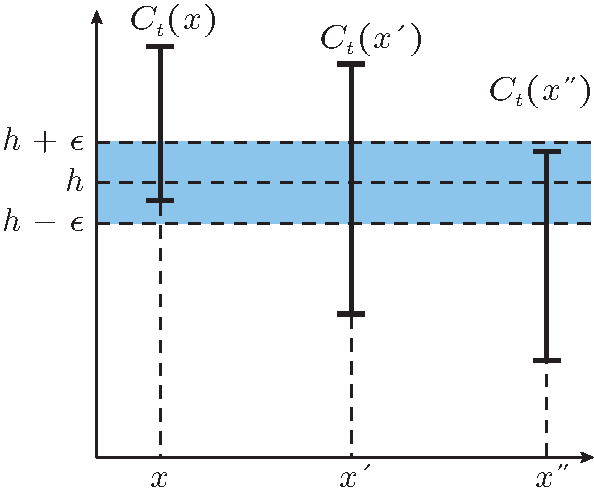
\includegraphics[height=1.7in]{figures/ch02/class}
    \caption{Confidence regions}
    \label{fig:conf}
  \end{subfigure}
  \hfill
  \begin{subfigure}[b]{0.49\linewidth}
    \centering
    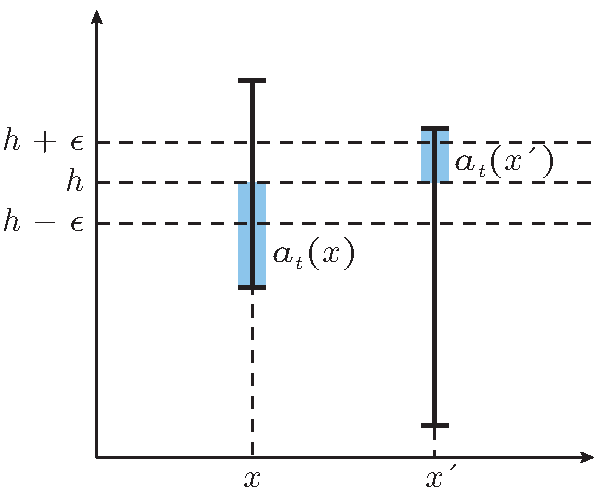
\includegraphics[height=1.7in]{figures/ch02/amb}
    \caption{Ambiguities}
    \label{fig:amb}
  \end{subfigure}
  \caption{
    \textbf{(a)} Example of the three possible configurations of confidence
    regions: $\*x$ will be classified into $H_t$, $\*x''$ into $L_t$, whereas
    $\*x'$ will remain unclassified.
    \textbf{(b)} Ambiguities of two example points: $\*x$ is a point of high
    ambiguity (close to $w_t(\*x)/2$), while $\*x'$ has low ambiguity (close to
    $\epsilon$).
  }
\end{figure}

\paragraph{Sample selection}
For selecting the next point to be evaluated at each iteration, we define the
following quantity
\begin{align*}
a_t(\*x) = \min\{\max(C_t(\*x)) - h, h - \min(C_t(\*x))\},
\end{align*}
which we call classification \emph{ambiguity}. As its name suggests, the
ambiguity of a point $\*x$ quantifies our uncertainty about whether $\*x$
belongs to $H_t$ or $L_t$.
The intuition of sampling at areas of the sample space with large
classification uncertainty, expecting to gain more information about
the problem at hand when sampling at those areas, manifests itself in \acl
by choosing to evaluate at each iteration the point with the largest
ambiguity amongst the yet unclassified.

Note that, if we define the confidence region \emph{width} of a point $\*x$ as
\begin{align*}
w_t(\*x) = \max(C_t(\*x)) - \min(C_t(\*x)),
\end{align*}
it follows from the the classification rules of \acl that
\begin{align*}
\epsilon \leq a_t(\*x) \leq w_t(\*x)/2,\ \text{for every}\ \*x\in U_t.
\end{align*}
Ambiguity values close to $w_t(\*x)/2$ indicate that the confidence region of
$\*x$ extends almost equally above and below the threshold level $h$, while
values close to $\epsilon$ indicate that $\*x$ can almost unambiguously
be classified
into $H_t$ or $L_t$ (see \figref{fig:amb}).

We can make an interesting observation at this point. If we use the confidence
intervals $Q_t(\*x)$ instead of the confidence regions $C_t(\*x)$
in the definition of ambiguity, we get the following quantity
\begin{align*}
a'_t(\*x) &= \min\{\max(Q_t(\*x)) - h, h - \min(Q_t(\*x))\}\\
          &= \min\{\mu_{t-1}(\*x) + \beta_t^{1/2}\sigma_{t-1}(\*x) - h,\ h - \mu_{t-1}(\*x) + \beta_t^{1/2}\sigma_{t-1}(\*x)\}\\
          &= \beta_t^{1/2}\sigma_{t-1}(\*x) - |\mu_{t-1}(\*x) - h|.
\end{align*}
For $\beta_t^{1/2} = 1.96$, this is identical to
the \emph{straddle}~\cite{bryan05} heuristic, which can thus be
intuitively explained in terms of classification ambiguity.

%\setlength\figureheight{1.5in}\setlength\figurewidth{2.5in}
%% This file was created by matlab2tikz v0.2.3.
% Copyright (c) 2008--2012, Nico Schlömer <nico.schloemer@gmail.com>
% All rights reserved.
% 
% 
%

\definecolor{locol}{rgb}{0.26, 0.45, 0.65}

\begin{tikzpicture}

\begin{axis}[%
tick label style={font=\tiny},
label style={font=\tiny},
xlabel shift={-10pt},
ylabel shift={-17pt},
legend style={font=\tiny},
view={0}{90},
width=\figurewidth,
height=\figureheight,
scale only axis,
xmin=0, xmax=1478,
xtick={0, 400, 1000, 1400},
xlabel={Length (m)},
ymin=-18, ymax=0,
ytick={0, -4, -14, -18},
ylabel={Depth (m)},
name=plot1,
axis lines*=box,
tickwidth=0.1cm,
clip=false
]

\addplot [fill=locol,draw=none,forget plot] coordinates{ (1478,0)(1478,-0.0602006688963211)(1478,-0.120401337792642)(1478,-0.180602006688963)(1478,-0.240802675585284)(1478,-0.301003344481605)(1478,-0.361204013377926)(1478,-0.421404682274247)(1478,-0.481605351170569)(1478,-0.54180602006689)(1478,-0.602006688963211)(1478,-0.662207357859532)(1478,-0.722408026755853)(1478,-0.782608695652174)(1478,-0.842809364548495)(1478,-0.903010033444816)(1478,-0.963210702341137)(1478,-1.02341137123746)(1478,-1.08361204013378)(1478,-1.1438127090301)(1478,-1.20401337792642)(1478,-1.26421404682274)(1478,-1.32441471571906)(1478,-1.38461538461538)(1478.00008238436,-1.44481605351171)(1478.00016476597,-1.50501672240803)(1478.00024714483,-1.56521739130435)(1478.00024714483,-1.62541806020067)(1478.00024714483,-1.68561872909699)(1478.00024714483,-1.74581939799331)(1478.00024714483,-1.80602006688963)(1478.00024714483,-1.86622073578595)(1478.00024714483,-1.92642140468227)(1478.00024714483,-1.9866220735786)(1478.00024714483,-2.04682274247492)(1478.00024714483,-2.10702341137124)(1478.00024714483,-2.16722408026756)(1478.00024714483,-2.22742474916388)(1478.00024714483,-2.2876254180602)(1478.00024714483,-2.34782608695652)(1478.00024714483,-2.40802675585284)(1478.00024714483,-2.46822742474916)(1478.00024714483,-2.52842809364549)(1478.00024714483,-2.58862876254181)(1478.00024714483,-2.64882943143813)(1478.00024714483,-2.70903010033445)(1478.00024714483,-2.76923076923077)(1478.00024714483,-2.82943143812709)(1478.00024714483,-2.88963210702341)(1478.00024714483,-2.94983277591973)(1478.00024714483,-3.01003344481605)(1478.00024714483,-3.07023411371237)(1478.00024714483,-3.1304347826087)(1478.00030206255,-3.19063545150502)(1478.00030206255,-3.25083612040134)(1478.00030206255,-3.31103678929766)(1478.00024714483,-3.37123745819398)(1478.00024714483,-3.4314381270903)(1478.00024714483,-3.49163879598662)(1478.00024714483,-3.55183946488294)(1478.00024714483,-3.61204013377926)(1478.00024714483,-3.67224080267559)(1478.00024714483,-3.73244147157191)(1478.00024714483,-3.79264214046823)(1478.00024714483,-3.85284280936455)(1478.00024714483,-3.91304347826087)(1478.00024714483,-3.97324414715719)(1478.00024714483,-4.03344481605351)(1478.00024714483,-4.09364548494983)(1478.00024714483,-4.15384615384615)(1478.00024714483,-4.21404682274247)(1478.00024714483,-4.2742474916388)(1478.00024714483,-4.33444816053512)(1478.00030206255,-4.39464882943144)(1478.00030206255,-4.45484949832776)(1478.00030206255,-4.51505016722408)(1478.00024714483,-4.5752508361204)(1478.00024714483,-4.63545150501672)(1478.00024714483,-4.69565217391304)(1478.00024714483,-4.75585284280936)(1478.00024714483,-4.81605351170569)(1478.00024714483,-4.87625418060201)(1478.00024714483,-4.93645484949833)(1478.00024714483,-4.99665551839465)(1478.00024714483,-5.05685618729097)(1478.0001922259,-5.11705685618729)(1478.0001922259,-5.17725752508361)(1478.0001922259,-5.23745819397993)(1478.00024714483,-5.29765886287625)(1478.00024714483,-5.35785953177258)(1478.00024714483,-5.4180602006689)(1478.00024714483,-5.47826086956522)(1478.00024714483,-5.53846153846154)(1478.00024714483,-5.59866220735786)(1478.00024714483,-5.65886287625418)(1478.00024714483,-5.7190635451505)(1478.00021968552,-5.77926421404682)(1478.0001922259,-5.83946488294314)(1478.0001098452,-5.89966555183946)(1478.00005492321,-5.95986622073579)(1478,-6.02006688963211)(1478,-6.08026755852843)(1478,-6.14046822742475)(1478,-6.20066889632107)(1478,-6.26086956521739)(1478,-6.32107023411371)(1478,-6.38127090301003)(1478,-6.44147157190635)(1478,-6.50167224080268)(1478,-6.561872909699)(1478.00002746176,-6.62207357859532)(1478.0001098452,-6.68227424749164)(1478.0001922259,-6.74247491638796)(1478.00024714483,-6.80267558528428)(1478.00024714483,-6.8628762541806)(1478.00024714483,-6.92307692307692)(1478.00024714483,-6.98327759197324)(1478.00024714483,-7.04347826086957)(1478.00024714483,-7.10367892976589)(1478.00024714483,-7.16387959866221)(1478.00024714483,-7.22408026755853)(1478.00024714483,-7.28428093645485)(1478.00024714483,-7.34448160535117)(1478.00024714483,-7.40468227424749)(1478.00024714483,-7.46488294314381)(1478.00024714483,-7.52508361204013)(1478.00024714483,-7.58528428093646)(1478.00024714483,-7.64548494983278)(1478.00024714483,-7.7056856187291)(1478.00024714483,-7.76588628762542)(1478.00024714483,-7.82608695652174)(1478.00024714483,-7.88628762541806)(1478.00024714483,-7.94648829431438)(1478.00024714483,-8.0066889632107)(1478.00024714483,-8.06688963210702)(1478.0001922259,-8.12709030100334)(1478.0001922259,-8.18729096989967)(1478.0001922259,-8.24749163879599)(1478.00024714483,-8.30769230769231)(1478.00024714483,-8.36789297658863)(1478.00024714483,-8.42809364548495)(1478.00024714483,-8.48829431438127)(1478.00024714483,-8.54849498327759)(1478.00024714483,-8.60869565217391)(1478.00024714483,-8.66889632107023)(1478.00024714483,-8.72909698996656)(1478.00024714483,-8.78929765886288)(1478.00024714483,-8.8494983277592)(1478.00024714483,-8.90969899665552)(1478.00024714483,-8.96989966555184)(1478.00024714483,-9.03010033444816)(1478.00024714483,-9.09030100334448)(1478.00024714483,-9.1505016722408)(1478.00024714483,-9.21070234113712)(1478.00024714483,-9.27090301003344)(1478.00024714483,-9.33110367892977)(1478.00024714483,-9.39130434782609)(1478.00024714483,-9.45150501672241)(1478.00024714483,-9.51170568561873)(1478.00024714483,-9.57190635451505)(1478.00024714483,-9.63210702341137)(1478.00024714483,-9.69230769230769)(1478.00024714483,-9.75250836120401)(1478.00024714483,-9.81270903010033)(1478.00024714483,-9.87290969899666)(1478.00024714483,-9.93311036789298)(1478.00024714483,-9.9933110367893)(1478.00024714483,-10.0535117056856)(1478.0001922259,-10.1137123745819)(1478.0001922259,-10.1739130434783)(1478.0001922259,-10.2341137123746)(1478.00024714483,-10.2943143812709)(1478.00024714483,-10.3545150501672)(1478.00024714483,-10.4147157190635)(1478.00024714483,-10.4749163879599)(1478.00024714483,-10.5351170568562)(1478.00024714483,-10.5953177257525)(1478.00024714483,-10.6555183946488)(1478.00024714483,-10.7157190635452)(1478.00024714483,-10.7759197324415)(1478.00024714483,-10.8361204013378)(1478.00024714483,-10.8963210702341)(1478.00024714483,-10.9565217391304)(1478.00024714483,-11.0167224080268)(1478.00024714483,-11.0769230769231)(1478.00024714483,-11.1371237458194)(1478.00024714483,-11.1973244147157)(1478.00024714483,-11.257525083612)(1478.00024714483,-11.3177257525084)(1478.00024714483,-11.3779264214047)(1478.00024714483,-11.438127090301)(1478.00024714483,-11.4983277591973)(1478.00024714483,-11.5585284280936)(1478.00016476597,-11.61872909699)(1478.00008238436,-11.6789297658863)(1478,-11.7391304347826)(1478,-11.7993311036789)(1478,-11.8595317725753)(1478,-11.9197324414716)(1478,-11.9799331103679)(1478,-12.0401337792642)(1478,-12.1003344481605)(1478,-12.1605351170569)(1478,-12.2207357859532)(1478,-12.2809364548495)(1478,-12.3411371237458)(1478,-12.4013377926421)(1478,-12.4615384615385)(1478,-12.5217391304348)(1478,-12.5819397993311)(1478,-12.6421404682274)(1478,-12.7023411371237)(1478,-12.7625418060201)(1478,-12.8227424749164)(1478,-12.8829431438127)(1478,-12.943143812709)(1478,-13.0033444816054)(1478,-13.0635451505017)(1478,-13.123745819398)(1478,-13.1839464882943)(1478,-13.2441471571906)(1478,-13.304347826087)(1478,-13.3645484949833)(1478,-13.4247491638796)(1478,-13.4849498327759)(1478,-13.5451505016722)(1478,-13.6053511705686)(1478,-13.6655518394649)(1478,-13.7257525083612)(1478,-13.7859531772575)(1478,-13.8461538461538)(1478,-13.9063545150502)(1478,-13.9665551839465)(1478,-14.0267558528428)(1478,-14.0869565217391)(1478,-14.1471571906355)(1478,-14.2073578595318)(1478,-14.2675585284281)(1478,-14.3277591973244)(1478,-14.3879598662207)(1478,-14.4481605351171)(1478,-14.5083612040134)(1478,-14.5685618729097)(1478,-14.628762541806)(1478,-14.6889632107023)(1478,-14.7491638795987)(1478,-14.809364548495)(1478,-14.8695652173913)(1478,-14.9297658862876)(1478,-14.9899665551839)(1478,-15.0501672240803)(1478,-15.1103678929766)(1478,-15.1705685618729)(1478,-15.2307692307692)(1478,-15.2909698996656)(1478,-15.3511705685619)(1478,-15.4113712374582)(1478,-15.4715719063545)(1478,-15.5317725752508)(1478,-15.5919732441472)(1478,-15.6521739130435)(1478,-15.7123745819398)(1478,-15.7725752508361)(1478,-15.8327759197324)(1478,-15.8929765886288)(1478,-15.9531772575251)(1478,-16.0133779264214)(1478,-16.0735785953177)(1478,-16.133779264214)(1478,-16.1939799331104)(1478,-16.2541806020067)(1478,-16.314381270903)(1478,-16.3745819397993)(1478,-16.4347826086957)(1478,-16.494983277592)(1478,-16.5551839464883)(1478,-16.6153846153846)(1478,-16.6755852842809)(1478,-16.7357859531773)(1478,-16.7959866220736)(1478,-16.8561872909699)(1478,-16.9163879598662)(1478,-16.9765886287625)(1478,-17.0367892976589)(1478,-17.0969899665552)(1478,-17.1571906354515)(1478,-17.2173913043478)(1478,-17.2775919732441)(1478,-17.3377926421405)(1478,-17.3979933110368)(1478,-17.4581939799331)(1478,-17.5183946488294)(1478,-17.5785953177258)(1478,-17.6387959866221)(1478,-17.6989966555184)(1478,-17.7591973244147)(1478,-17.819397993311)(1478,-17.8795986622074)(1478,-17.9397993311037)(1478,-18)(1473.05685618729,-18)(1468.11371237458,-18)(1463.17056856187,-18)(1458.22742474916,-18)(1453.28428093645,-18)(1448.34113712375,-18)(1443.39799331104,-18)(1438.45484949833,-18)(1433.51170568562,-18)(1428.56856187291,-18)(1423.6254180602,-18)(1418.68227424749,-18)(1413.73913043478,-18)(1408.79598662207,-18)(1403.85284280936,-18)(1398.90969899666,-18)(1393.96655518395,-18)(1389.02341137124,-18)(1384.08026755853,-18)(1379.13712374582,-18)(1374.19397993311,-18)(1369.2508361204,-18)(1364.30769230769,-18)(1359.36454849498,-18)(1354.42140468227,-18)(1349.47826086957,-18)(1344.53511705686,-18)(1339.59197324415,-18)(1334.64882943144,-18)(1329.70568561873,-18)(1324.76254180602,-18)(1319.81939799331,-18)(1314.8762541806,-18)(1309.93311036789,-18)(1304.98996655518,-18)(1300.04682274247,-18)(1295.10367892977,-18)(1290.16053511706,-18)(1285.21739130435,-18)(1280.27424749164,-18)(1275.33110367893,-18)(1270.38795986622,-18)(1265.44481605351,-18)(1260.5016722408,-18)(1255.55852842809,-18)(1250.61538461538,-18)(1245.67224080268,-18)(1240.72909698997,-18)(1235.78595317726,-18)(1230.84280936455,-18)(1225.89966555184,-18)(1220.95652173913,-18)(1216.01337792642,-18)(1211.07023411371,-18)(1206.127090301,-18)(1201.18394648829,-18)(1196.24080267559,-18)(1191.29765886288,-18)(1186.35451505017,-18)(1181.41137123746,-18)(1176.46822742475,-18)(1171.52508361204,-18)(1166.58193979933,-18)(1161.63879598662,-18)(1156.69565217391,-18)(1151.7525083612,-18)(1146.8093645485,-18)(1141.86622073579,-18)(1136.92307692308,-18)(1131.97993311037,-18)(1127.03678929766,-18)(1122.09364548495,-18)(1117.15050167224,-18)(1112.20735785953,-18)(1107.26421404682,-18)(1102.32107023411,-18)(1097.3779264214,-18)(1092.4347826087,-18)(1087.49163879599,-18)(1082.54849498328,-18)(1077.60535117057,-18)(1072.66220735786,-18)(1067.71906354515,-18)(1062.77591973244,-18)(1057.83277591973,-18)(1052.88963210702,-18)(1047.94648829431,-18)(1043.00334448161,-18)(1038.0602006689,-18)(1033.11705685619,-18)(1028.17391304348,-18)(1023.23076923077,-18)(1018.28762541806,-18)(1013.34448160535,-18)(1008.40133779264,-18)(1003.45819397993,-18)(998.515050167224,-18)(993.571906354515,-18)(988.628762541806,-18)(983.685618729097,-18)(978.742474916388,-18)(973.799331103679,-18)(968.85618729097,-18)(963.913043478261,-18)(958.969899665552,-18)(954.026755852843,-18)(949.083612040134,-18)(944.140468227425,-18)(939.197324414716,-18)(934.254180602007,-18)(929.311036789298,-18)(924.367892976589,-18)(919.42474916388,-18)(914.481605351171,-18)(909.538461538462,-18)(904.595317725752,-18)(899.652173913044,-18)(894.709030100334,-18)(889.765886287625,-18)(884.822742474916,-18)(879.879598662207,-18)(874.936454849498,-18)(869.993311036789,-18)(865.05016722408,-18)(860.107023411371,-18)(855.163879598662,-18)(850.220735785953,-18)(845.277591973244,-18)(840.334448160535,-18)(835.391304347826,-18)(830.448160535117,-18)(825.505016722408,-18)(820.561872909699,-18)(815.61872909699,-18)(810.675585284281,-18)(805.732441471572,-18)(800.789297658863,-18)(795.846153846154,-18)(790.903010033445,-18)(785.959866220736,-18)(781.016722408027,-18)(776.073578595318,-18)(771.130434782609,-18)(766.1872909699,-18)(761.244147157191,-18)(756.301003344482,-18)(751.357859531773,-18)(746.414715719064,-18)(741.471571906354,-18)(736.528428093646,-18)(731.585284280936,-18)(726.642140468227,-18)(721.698996655518,-18)(716.755852842809,-18)(711.8127090301,-18)(706.869565217391,-18)(701.926421404682,-18)(696.983277591973,-18)(692.040133779264,-18)(687.096989966555,-18)(682.153846153846,-18)(677.210702341137,-18)(672.267558528428,-18)(667.324414715719,-18)(662.38127090301,-18)(657.438127090301,-18)(652.494983277592,-18)(647.551839464883,-18)(642.608695652174,-18)(637.665551839465,-18)(632.722408026756,-18)(627.779264214047,-18)(622.836120401338,-18)(617.892976588629,-18)(612.94983277592,-18)(608.006688963211,-18)(603.063545150502,-18)(598.120401337793,-18)(593.177257525084,-18)(588.234113712375,-18)(583.290969899666,-18)(578.347826086957,-18)(573.404682274248,-18)(568.461538461538,-18)(563.518394648829,-18)(558.57525083612,-18)(553.632107023411,-18)(548.688963210702,-18)(543.745819397993,-18)(538.802675585284,-18)(533.859531772575,-18)(528.916387959866,-18)(523.973244147157,-18)(519.030100334448,-18)(514.086956521739,-18)(509.14381270903,-18)(504.200668896321,-18)(499.257525083612,-18)(494.314381270903,-18)(489.371237458194,-18)(484.428093645485,-18)(479.484949832776,-18)(474.541806020067,-18)(469.598662207358,-18)(464.655518394649,-18)(459.71237458194,-18)(454.769230769231,-18)(449.826086956522,-18)(444.882943143813,-18)(439.939799331104,-18)(434.996655518395,-18)(430.053511705686,-18)(425.110367892977,-18)(420.167224080268,-18)(415.224080267559,-18)(410.28093645485,-18)(405.33779264214,-18)(400.394648829431,-18)(395.451505016722,-18)(390.508361204013,-18)(385.565217391304,-18)(380.622073578595,-18)(375.678929765886,-18)(370.735785953177,-18)(365.792642140468,-18)(360.849498327759,-18)(355.90635451505,-18)(350.963210702341,-18)(346.020066889632,-18)(341.076923076923,-18)(336.133779264214,-18)(331.190635451505,-18)(326.247491638796,-18)(321.304347826087,-18)(316.361204013378,-18)(311.418060200669,-18)(306.47491638796,-18)(301.531772575251,-18)(296.588628762542,-18)(291.645484949833,-18)(286.702341137124,-18)(281.759197324415,-18)(276.816053511706,-18)(271.872909698997,-18)(266.929765886288,-18)(261.986622073579,-18)(257.04347826087,-18)(252.100334448161,-18)(247.157190635452,-18)(242.214046822742,-18)(237.270903010033,-18)(232.327759197324,-18)(227.384615384615,-18)(222.441471571906,-18)(217.498327759197,-18)(212.555183946488,-18)(207.612040133779,-18)(202.66889632107,-18)(197.725752508361,-18)(192.782608695652,-18)(187.839464882943,-18)(182.896321070234,-18)(177.953177257525,-18)(173.010033444816,-18)(168.066889632107,-18)(163.123745819398,-18)(158.180602006689,-18)(153.23745819398,-18)(148.294314381271,-18)(143.351170568562,-18)(138.408026755853,-18)(133.464882943144,-18)(128.521739130435,-18)(123.578595317726,-18)(118.635451505017,-18)(113.692307692308,-18)(108.749163879599,-18)(103.80602006689,-18)(98.8628762541806,-18)(93.9197324414716,-18)(88.9765886287625,-18)(84.0334448160535,-18)(79.0903010033445,-18)(74.1471571906355,-18)(69.2040133779264,-18)(64.2608695652174,-18)(59.3177257525084,-18)(54.3745819397993,-18)(49.4314381270903,-18)(44.4882943143813,-18)(39.5451505016722,-18)(34.6020066889632,-18)(29.6588628762542,-18)(24.7157190635452,-18)(19.7725752508361,-18)(14.8294314381271,-18)(9.88628762541806,-18)(4.94314381270903,-18)(0,-18)(0,-17.9397993311037)(0,-17.8795986622074)(0,-17.819397993311)(0,-17.7591973244147)(0,-17.6989966555184)(0,-17.6387959866221)(0,-17.5785953177258)(0,-17.5183946488294)(0,-17.4581939799331)(0,-17.3979933110368)(0,-17.3377926421405)(0,-17.2775919732441)(0,-17.2173913043478)(0,-17.1571906354515)(0,-17.0969899665552)(0,-17.0367892976589)(0,-16.9765886287625)(0,-16.9163879598662)(0,-16.8561872909699)(0,-16.7959866220736)(0,-16.7357859531773)(0,-16.6755852842809)(0,-16.6153846153846)(0,-16.5551839464883)(0,-16.494983277592)(0,-16.4347826086957)(0,-16.3745819397993)(0,-16.314381270903)(0,-16.2541806020067)(0,-16.1939799331104)(0,-16.133779264214)(0,-16.0735785953177)(0,-16.0133779264214)(0,-15.9531772575251)(0,-15.8929765886288)(0,-15.8327759197324)(0,-15.7725752508361)(0,-15.7123745819398)(0,-15.6521739130435)(0,-15.5919732441472)(0,-15.5317725752508)(0,-15.4715719063545)(0,-15.4113712374582)(0,-15.3511705685619)(0,-15.2909698996656)(0,-15.2307692307692)(0,-15.1705685618729)(0,-15.1103678929766)(0,-15.0501672240803)(0,-14.9899665551839)(0,-14.9297658862876)(0,-14.8695652173913)(0,-14.809364548495)(0,-14.7491638795987)(0,-14.6889632107023)(0,-14.628762541806)(0,-14.5685618729097)(0,-14.5083612040134)(0,-14.4481605351171)(0,-14.3879598662207)(0,-14.3277591973244)(0,-14.2675585284281)(0,-14.2073578595318)(0,-14.1471571906355)(0,-14.0869565217391)(0,-14.0267558528428)(0,-13.9665551839465)(0,-13.9063545150502)(0,-13.8461538461538)(0,-13.7859531772575)(0,-13.7257525083612)(0,-13.6655518394649)(0,-13.6053511705686)(0,-13.5451505016722)(0,-13.4849498327759)(0,-13.4247491638796)(0,-13.3645484949833)(0,-13.304347826087)(0,-13.2441471571906)(0,-13.1839464882943)(0,-13.123745819398)(0,-13.0635451505017)(0,-13.0033444816054)(0,-12.943143812709)(0,-12.8829431438127)(0,-12.8227424749164)(0,-12.7625418060201)(0,-12.7023411371237)(0,-12.6421404682274)(0,-12.5819397993311)(0,-12.5217391304348)(0,-12.4615384615385)(0,-12.4013377926421)(0,-12.3411371237458)(0,-12.2809364548495)(0,-12.2207357859532)(0,-12.1605351170569)(0,-12.1003344481605)(0,-12.0401337792642)(0,-11.9799331103679)(0,-11.9197324414716)(0,-11.8595317725753)(0,-11.7993311036789)(0,-11.7391304347826)(0,-11.6789297658863)(0,-11.61872909699)(0,-11.5585284280936)(0,-11.4983277591973)(0,-11.438127090301)(0,-11.3779264214047)(0,-11.3177257525084)(0,-11.257525083612)(0,-11.1973244147157)(0,-11.1371237458194)(0,-11.0769230769231)(0,-11.0167224080268)(0,-10.9565217391304)(0,-10.8963210702341)(0,-10.8361204013378)(0,-10.7759197324415)(0,-10.7157190635452)(0,-10.6555183946488)(0,-10.5953177257525)(0,-10.5351170568562)(0,-10.4749163879599)(0,-10.4147157190635)(0,-10.3545150501672)(0,-10.2943143812709)(0,-10.2341137123746)(-5.49232098834381e-05,-10.1739130434783)(-0.000137305736304806,-10.1137123745819)(-0.000219685516764337,-10.0535117056856)(-0.000247144833393367,-9.9933110367893)(-0.000247144833393367,-9.93311036789298)(-0.000247144833393367,-9.87290969899666)(-0.000247144833393367,-9.81270903010033)(-0.000247144833393367,-9.75250836120401)(-0.000247144833393367,-9.69230769230769)(-0.000247144833393367,-9.63210702341137)(-0.000247144833393367,-9.57190635451505)(-0.000302062551398134,-9.51170568561873)(-0.000302062551398134,-9.45150501672241)(-0.000302062551398134,-9.39130434782609)(-0.000247144833393367,-9.33110367892977)(-0.000247144833393367,-9.27090301003344)(-0.000274603844937234,-9.21070234113712)(-0.000302062551398134,-9.1505016722408)(-0.000384436840345592,-9.09030100334448)(-0.000439351507662275,-9.03010033444816)(-0.000439351507662275,-8.96989966555184)(-0.000384436840345592,-8.90969899665552)(-0.00032952095278375,-8.8494983277592)(-0.000302062551398134,-8.78929765886288)(-0.000274603844937234,-8.72909698996656)(-0.000247144833393367,-8.66889632107023)(-0.000247144833393367,-8.60869565217391)(-0.000247144833393367,-8.54849498327759)(-0.000247144833393367,-8.48829431438127)(-0.000247144833393367,-8.42809364548495)(-0.000247144833393367,-8.36789297658863)(-0.000247144833393367,-8.30769230769231)(-0.000247144833393367,-8.24749163879599)(-0.000247144833393367,-8.18729096989967)(-0.000247144833393367,-8.12709030100334)(-0.000247144833393367,-8.06688963210702)(-0.000247144833393367,-8.0066889632107)(-0.000247144833393367,-7.94648829431438)(-0.000247144833393367,-7.88628762541806)(-0.000247144833393367,-7.82608695652174)(-0.000247144833393367,-7.76588628762542)(-0.000247144833393367,-7.7056856187291)(-0.000247144833393367,-7.64548494983278)(-0.000247144833393367,-7.58528428093646)(-0.000247144833393367,-7.52508361204013)(-0.000247144833393367,-7.46488294314381)(-0.000247144833393367,-7.40468227424749)(-0.000247144833393367,-7.34448160535117)(-0.000247144833393367,-7.28428093645485)(-0.000247144833393367,-7.22408026755853)(-0.000247144833393367,-7.16387959866221)(-0.000247144833393367,-7.10367892976589)(-0.000247144833393367,-7.04347826086957)(-0.000247144833393367,-6.98327759197324)(-0.000247144833393367,-6.92307692307692)(-0.000247144833393367,-6.8628762541806)(-0.000247144833393367,-6.80267558528428)(-0.000247144833393367,-6.74247491638796)(-0.000247144833393367,-6.68227424749164)(-0.000247144833393367,-6.62207357859532)(-0.000247144833393367,-6.561872909699)(-0.000247144833393367,-6.50167224080268)(-0.000247144833393367,-6.44147157190635)(-0.000247144833393367,-6.38127090301003)(-0.000247144833393367,-6.32107023411371)(-0.000247144833393367,-6.26086956521739)(-0.000247144833393367,-6.20066889632107)(-0.000247144833393367,-6.14046822742475)(-0.000247144833393367,-6.08026755852843)(-0.000247144833393367,-6.02006688963211)(-0.000247144833393367,-5.95986622073579)(-0.000247144833393367,-5.89966555183946)(-0.000247144833393367,-5.83946488294314)(-0.000302062551398134,-5.77926421404682)(-0.000302062551398134,-5.7190635451505)(-0.000302062551398134,-5.65886287625418)(-0.000247144833393367,-5.59866220735786)(-0.000247144833393367,-5.53846153846154)(-0.000247144833393367,-5.47826086956522)(-0.000247144833393367,-5.4180602006689)(-0.000302062551398134,-5.35785953177258)(-0.000302062551398134,-5.29765886287625)(-0.000302062551398134,-5.23745819397993)(-0.000247144833393367,-5.17725752508361)(-0.000247144833393367,-5.11705685618729)(-0.000247144833393367,-5.05685618729097)(-0.000164765968224447,-4.99665551839465)(-8.23843571386917e-05,-4.93645484949833)(0,-4.87625418060201)(0,-4.81605351170569)(0,-4.75585284280936)(0,-4.69565217391304)(0,-4.63545150501672)(0,-4.5752508361204)(0,-4.51505016722408)(0,-4.45484949832776)(0,-4.39464882943144)(0,-4.33444816053512)(0,-4.2742474916388)(0,-4.21404682274247)(0,-4.15384615384615)(0,-4.09364548494983)(0,-4.03344481605351)(0,-3.97324414715719)(0,-3.91304347826087)(0,-3.85284280936455)(0,-3.79264214046823)(0,-3.73244147157191)(0,-3.67224080267559)(0,-3.61204013377926)(0,-3.55183946488294)(0,-3.49163879598662)(0,-3.4314381270903)(0,-3.37123745819398)(0,-3.31103678929766)(-8.23843571386917e-05,-3.25083612040134)(-0.00010984519927805,-3.19063545150502)(-0.000192225895042461,-3.1304347826087)(-0.000192225895042461,-3.07023411371237)(-0.000247144833393367,-3.01003344481605)(-0.000247144833393367,-2.94983277591973)(-0.000247144833393367,-2.88963210702341)(-0.000247144833393367,-2.82943143812709)(-0.000247144833393367,-2.76923076923077)(-0.000247144833393367,-2.70903010033445)(-0.000247144833393367,-2.64882943143813)(-0.000247144833393367,-2.58862876254181)(-0.000247144833393367,-2.52842809364549)(-0.000247144833393367,-2.46822742474916)(-0.000247144833393367,-2.40802675585284)(-0.000247144833393367,-2.34782608695652)(-0.000247144833393367,-2.2876254180602)(-0.000247144833393367,-2.22742474916388)(-0.000247144833393367,-2.16722408026756)(-0.000247144833393367,-2.10702341137124)(-0.000247144833393367,-2.04682274247492)(-0.000247144833393367,-1.9866220735786)(-0.000247144833393367,-1.92642140468227)(-0.000247144833393367,-1.86622073578595)(-0.000247144833393367,-1.80602006688963)(-0.000247144833393367,-1.74581939799331)(-0.000247144833393367,-1.68561872909699)(-0.000247144833393367,-1.62541806020067)(-0.000247144833393367,-1.56521739130435)(-0.000247144833393367,-1.50501672240803)(-0.000247144833393367,-1.44481605351171)(-0.000247144833393367,-1.38461538461538)(-0.000164765968224447,-1.32441471571906)(-8.23843571386917e-05,-1.26421404682274)(0,-1.20401337792642)(0,-1.1438127090301)(0,-1.08361204013378)(0,-1.02341137123746)(0,-0.963210702341137)(0,-0.903010033444816)(0,-0.842809364548495)(0,-0.782608695652174)(0,-0.722408026755853)(0,-0.662207357859532)(0,-0.602006688963211)(0,-0.54180602006689)(0,-0.481605351170569)(0,-0.421404682274247)(0,-0.361204013377926)(0,-0.301003344481605)(0,-0.240802675585284)(0,-0.180602006688963)(0,-0.120401337792642)(0,-0.0602006688963211)(0,0)(4.94314381270903,0)(9.88628762541806,0)(14.8294314381271,0)(19.7725752508361,0)(24.7157190635452,0)(29.6588628762542,0)(34.6020066889632,0)(39.5451505016722,0)(44.4882943143813,0)(49.4314381270903,0)(54.3745819397993,0)(59.3177257525084,0)(64.2608695652174,0)(69.2040133779264,0)(74.1471571906355,0)(79.0903010033445,0)(84.0334448160535,0)(88.9765886287625,0)(93.9197324414716,0)(98.8628762541806,0)(103.80602006689,0)(108.749163879599,0)(113.692307692308,0)(118.635451505017,0)(123.578595317726,0)(128.521739130435,0)(133.464882943144,0)(138.408026755853,0)(143.351170568562,0)(148.294314381271,0)(153.23745819398,0)(158.180602006689,0)(163.123745819398,0)(168.066889632107,0)(173.010033444816,0)(177.953177257525,0)(182.896321070234,0)(187.839464882943,0)(192.782608695652,0)(197.725752508361,0)(202.66889632107,0)(207.612040133779,0)(212.555183946488,0)(217.498327759197,0)(222.441471571906,0)(227.384615384615,0)(232.327759197324,0)(237.270903010033,0)(242.214046822742,0)(247.157190635452,0)(252.100334448161,0)(257.04347826087,6.68888888972859e-07)(261.986622073579,1.33776291406302e-06)(266.929765886288,2.34104608306109e-06)(271.872909698997,2.67546637465379e-06)(276.816053511706,3.00988295066346e-06)(281.759197324415,3.00988295066346e-06)(286.702341137124,3.00988295066346e-06)(291.645484949833,3.00988295066346e-06)(296.588628762542,3.00988295066346e-06)(301.531772575251,3.00988295066346e-06)(306.47491638796,3.00988295066346e-06)(311.418060200669,3.00988295066346e-06)(316.361204013378,3.00988295066346e-06)(321.304347826087,3.00988295066346e-06)(326.247491638796,3.00988295066346e-06)(331.190635451505,3.00988295066346e-06)(336.133779264214,3.00988295066346e-06)(341.076923076923,3.00988295066346e-06)(346.020066889632,3.00988295066346e-06)(350.963210702341,3.00988295066346e-06)(355.90635451505,3.00988295066346e-06)(360.849498327759,3.00988295066346e-06)(365.792642140468,3.00988295066346e-06)(370.735785953177,3.00988295066346e-06)(375.678929765886,3.00988295066346e-06)(380.622073578595,3.00988295066346e-06)(385.565217391304,3.00988295066346e-06)(390.508361204013,3.00988295066346e-06)(395.451505016722,3.00988295066346e-06)(400.394648829431,3.00988295066346e-06)(405.33779264214,3.00988295066346e-06)(410.28093645485,3.00988295066346e-06)(415.224080267559,3.00988295066346e-06)(420.167224080268,3.00988295066346e-06)(425.110367892977,3.00988295066346e-06)(430.053511705686,3.00988295066346e-06)(434.996655518395,3.00988295066346e-06)(439.939799331104,3.00988295066346e-06)(444.882943143813,3.00988295066346e-06)(449.826086956522,3.00988295066346e-06)(454.769230769231,3.00988295066346e-06)(459.71237458194,3.00988295066346e-06)(464.655518394649,3.00988295066346e-06)(469.598662207358,3.00988295066346e-06)(474.541806020067,3.00988295066346e-06)(479.484949832776,3.00988295066346e-06)(484.428093645485,3.00988295066346e-06)(489.371237458194,3.00988295066346e-06)(494.314381270903,3.00988295066346e-06)(499.257525083612,3.00988295066346e-06)(504.200668896321,3.00988295066346e-06)(509.14381270903,3.00988295066346e-06)(514.086956521739,3.00988295066346e-06)(519.030100334448,3.00988295066346e-06)(523.973244147157,3.00988295066346e-06)(528.916387959866,3.00988295066346e-06)(533.859531772575,3.00988295066346e-06)(538.802675585284,2.67546637465379e-06)(543.745819397993,2.34104608306109e-06)(548.688963210702,1.33776291406302e-06)(553.632107023411,6.68888888972859e-07)(558.57525083612,0)(563.518394648829,0)(568.461538461538,0)(573.404682274248,0)(578.347826086957,0)(583.290969899666,0)(588.234113712375,0)(593.177257525084,0)(598.120401337793,0)(603.063545150502,0)(608.006688963211,0)(612.94983277592,0)(617.892976588629,0)(622.836120401338,0)(627.779264214047,0)(632.722408026756,0)(637.665551839465,0)(642.608695652174,0)(647.551839464883,0)(652.494983277592,0)(657.438127090301,0)(662.38127090301,0)(667.324414715719,0)(672.267558528428,0)(677.210702341137,0)(682.153846153846,0)(687.096989966555,0)(692.040133779264,0)(696.983277591973,0)(701.926421404682,0)(706.869565217391,0)(711.8127090301,0)(716.755852842809,0)(721.698996655518,0)(726.642140468227,0)(731.585284280936,0)(736.528428093646,0)(741.471571906354,0)(746.414715719064,0)(751.357859531773,0)(756.301003344482,0)(761.244147157191,0)(766.1872909699,0)(771.130434782609,0)(776.073578595318,0)(781.016722408027,0)(785.959866220736,0)(790.903010033445,0)(795.846153846154,0)(800.789297658863,0)(805.732441471572,0)(810.675585284281,0)(815.61872909699,0)(820.561872909699,0)(825.505016722408,0)(830.448160535117,0)(835.391304347826,0)(840.334448160535,0)(845.277591973244,0)(850.220735785953,0)(855.163879598662,0)(860.107023411371,0)(865.05016722408,0)(869.993311036789,0)(874.936454849498,0)(879.879598662207,0)(884.822742474916,0)(889.765886287625,0)(894.709030100334,0)(899.652173913044,0)(904.595317725752,0)(909.538461538462,0)(914.481605351171,0)(919.42474916388,0)(924.367892976589,0)(929.311036789298,0)(934.254180602007,0)(939.197324414716,0)(944.140468227425,0)(949.083612040134,0)(954.026755852843,0)(958.969899665552,0)(963.913043478261,0)(968.85618729097,0)(973.799331103679,0)(978.742474916388,0)(983.685618729097,0)(988.628762541806,0)(993.571906354515,0)(998.515050167224,0)(1003.45819397993,0)(1008.40133779264,0)(1013.34448160535,0)(1018.28762541806,0)(1023.23076923077,0)(1028.17391304348,0)(1033.11705685619,0)(1038.0602006689,0)(1043.00334448161,0)(1047.94648829431,0)(1052.88963210702,0)(1057.83277591973,0)(1062.77591973244,0)(1067.71906354515,0)(1072.66220735786,0)(1077.60535117057,0)(1082.54849498328,0)(1087.49163879599,0)(1092.4347826087,0)(1097.3779264214,0)(1102.32107023411,0)(1107.26421404682,0)(1112.20735785953,0)(1117.15050167224,0)(1122.09364548495,0)(1127.03678929766,0)(1131.97993311037,0)(1136.92307692308,0)(1141.86622073579,0)(1146.8093645485,0)(1151.7525083612,0)(1156.69565217391,0)(1161.63879598662,0)(1166.58193979933,0)(1171.52508361204,0)(1176.46822742475,0)(1181.41137123746,0)(1186.35451505017,0)(1191.29765886288,0)(1196.24080267559,0)(1201.18394648829,0)(1206.127090301,0)(1211.07023411371,0)(1216.01337792642,0)(1220.95652173913,0)(1225.89966555184,0)(1230.84280936455,0)(1235.78595317726,0)(1240.72909698997,0)(1245.67224080268,0)(1250.61538461538,0)(1255.55852842809,0)(1260.5016722408,0)(1265.44481605351,0)(1270.38795986622,0)(1275.33110367893,0)(1280.27424749164,0)(1285.21739130435,0)(1290.16053511706,0)(1295.10367892977,0)(1300.04682274247,0)(1304.98996655518,0)(1309.93311036789,0)(1314.8762541806,0)(1319.81939799331,0)(1324.76254180602,0)(1329.70568561873,0)(1334.64882943144,0)(1339.59197324415,0)(1344.53511705686,0)(1349.47826086957,0)(1354.42140468227,0)(1359.36454849498,0)(1364.30769230769,0)(1369.2508361204,0)(1374.19397993311,0)(1379.13712374582,0)(1384.08026755853,0)(1389.02341137124,0)(1393.96655518395,0)(1398.90969899666,0)(1403.85284280936,0)(1408.79598662207,0)(1413.73913043478,0)(1418.68227424749,0)(1423.6254180602,0)(1428.56856187291,0)(1433.51170568562,0)(1438.45484949833,0)(1443.39799331104,0)(1448.34113712375,0)(1453.28428093645,0)(1458.22742474916,0)(1463.17056856187,0)(1468.11371237458,0)(1473.05685618729,0)(1478,0)};

\addplot [fill=darkgray,draw=none,forget plot] coordinates{ (6.17892976588629,-1.32441471571906)(9.88628762541806,-1.35451505016722)(13.5936454849498,-1.38461538461538)(14.8294314381271,-1.39464882943144)(19.7725752508361,-1.43478260869565)(21.0083612040134,-1.44481605351171)(24.7157190635452,-1.47491638795987)(27.1872909698997,-1.50501672240803)(29.6588628762542,-1.53511705685619)(33.366220735786,-1.56521739130435)(34.6020066889632,-1.5752508361204)(39.5451505016722,-1.61538461538462)(40.7809364548495,-1.62541806020067)(44.4882943143813,-1.65551839464883)(46.9598662207358,-1.68561872909699)(49.4314381270903,-1.71571906354515)(51.9030100334448,-1.74581939799331)(54.3745819397993,-1.77591973244147)(56.8461538461538,-1.80602006688963)(59.3177257525084,-1.83612040133779)(61.7892976588629,-1.86622073578595)(64.2608695652174,-1.91137123745819)(65.0847268673356,-1.92642140468227)(68.3801560758082,-1.9866220735786)(69.2040133779264,-2.00167224080268)(71.6755852842809,-2.04682274247492)(74.1471571906355,-2.07692307692308)(76.61872909699,-2.10702341137124)(79.0903010033445,-2.1371237458194)(81.561872909699,-2.16722408026756)(84.0334448160535,-2.19732441471572)(86.505016722408,-2.22742474916388)(88.9765886287625,-2.25752508361204)(92.6839464882943,-2.2876254180602)(93.9197324414716,-2.29765886287625)(98.8628762541806,-2.33779264214047)(101.334448160535,-2.34782608695652)(103.80602006689,-2.35785953177258)(108.749163879599,-2.39799331103679)(111.220735785953,-2.40802675585284)(113.692307692308,-2.4180602006689)(118.635451505017,-2.45819397993311)(121.107023411371,-2.46822742474916)(123.578595317726,-2.47826086956522)(128.521739130435,-2.49832775919732)(133.464882943144,-2.49832775919732)(138.408026755853,-2.49832775919732)(143.351170568562,-2.51839464882943)(145.822742474916,-2.52842809364549)(148.294314381271,-2.53846153846154)(153.23745819398,-2.55852842809365)(158.180602006689,-2.55852842809365)(163.123745819398,-2.55852842809365)(168.066889632107,-2.55852842809365)(173.010033444816,-2.55852842809365)(177.953177257525,-2.57859531772575)(180.42474916388,-2.58862876254181)(182.896321070234,-2.59866220735786)(187.839464882943,-2.61872909698997)(192.782608695652,-2.61872909698997)(197.725752508361,-2.61872909698997)(202.66889632107,-2.61872909698997)(207.612040133779,-2.61872909698997)(212.555183946488,-2.61872909698997)(217.498327759197,-2.61872909698997)(222.441471571906,-2.61872909698997)(227.384615384615,-2.61872909698997)(232.327759197324,-2.61872909698997)(237.270903010033,-2.61872909698997)(242.214046822742,-2.61872909698997)(247.157190635452,-2.61872909698997)(252.100334448161,-2.61872909698997)(257.04347826087,-2.61872909698997)(261.986622073579,-2.61872909698997)(266.929765886288,-2.61872909698997)(271.872909698997,-2.59866220735786)(274.344481605351,-2.58862876254181)(276.816053511706,-2.57859531772575)(281.759197324415,-2.55852842809365)(286.702341137124,-2.55852842809365)(291.645484949833,-2.55852842809365)(296.588628762542,-2.55852842809365)(301.531772575251,-2.53846153846154)(304.003344481605,-2.52842809364549)(306.47491638796,-2.51839464882943)(311.418060200669,-2.49832775919732)(316.361204013378,-2.49832775919732)(321.304347826087,-2.49832775919732)(326.247491638796,-2.49832775919732)(331.190635451505,-2.47826086956522)(333.66220735786,-2.46822742474916)(336.133779264214,-2.45819397993311)(341.076923076923,-2.438127090301)(346.020066889632,-2.438127090301)(350.963210702341,-2.438127090301)(355.90635451505,-2.438127090301)(360.849498327759,-2.438127090301)(365.792642140468,-2.4180602006689)(368.264214046823,-2.40802675585284)(370.735785953177,-2.39799331103679)(375.678929765886,-2.37792642140468)(380.622073578595,-2.37792642140468)(385.565217391304,-2.37792642140468)(390.508361204013,-2.37792642140468)(395.451505016722,-2.37792642140468)(400.394648829431,-2.37792642140468)(405.33779264214,-2.39799331103679)(407.809364548495,-2.40802675585284)(410.28093645485,-2.4180602006689)(415.224080267559,-2.438127090301)(420.167224080268,-2.438127090301)(425.110367892977,-2.438127090301)(430.053511705686,-2.438127090301)(434.996655518395,-2.438127090301)(439.939799331104,-2.45819397993311)(442.411371237458,-2.46822742474916)(444.882943143813,-2.47826086956522)(449.826086956522,-2.49832775919732)(454.769230769231,-2.49832775919732)(459.71237458194,-2.51839464882943)(462.183946488294,-2.52842809364549)(464.655518394649,-2.53846153846154)(469.598662207358,-2.55852842809365)(474.541806020067,-2.55852842809365)(479.484949832776,-2.57859531772575)(481.95652173913,-2.58862876254181)(484.428093645485,-2.59866220735786)(489.371237458194,-2.61872909698997)(494.314381270903,-2.63879598662207)(496.785953177258,-2.64882943143813)(499.257525083612,-2.65886287625418)(504.200668896321,-2.67892976588629)(509.14381270903,-2.69899665551839)(511.615384615385,-2.70903010033445)(514.086956521739,-2.7190635451505)(519.030100334448,-2.73913043478261)(523.973244147157,-2.73913043478261)(528.916387959866,-2.75919732441472)(531.387959866221,-2.76923076923077)(533.859531772575,-2.77926421404682)(538.802675585284,-2.79933110367893)(543.745819397993,-2.79933110367893)(548.688963210702,-2.81939799331104)(551.160535117057,-2.82943143812709)(553.632107023411,-2.83946488294314)(558.57525083612,-2.85953177257525)(563.518394648829,-2.85953177257525)(568.461538461538,-2.85953177257525)(573.404682274248,-2.87959866220736)(575.876254180602,-2.88963210702341)(578.347826086957,-2.89966555183946)(583.290969899666,-2.91973244147157)(588.234113712375,-2.91973244147157)(593.177257525084,-2.91973244147157)(598.120401337793,-2.91973244147157)(603.063545150502,-2.91973244147157)(608.006688963211,-2.91973244147157)(612.94983277592,-2.91973244147157)(617.892976588629,-2.91973244147157)(622.836120401338,-2.91973244147157)(627.779264214047,-2.89966555183946)(630.250836120401,-2.88963210702341)(632.722408026756,-2.87959866220736)(637.665551839465,-2.85953177257525)(642.608695652174,-2.83946488294314)(645.080267558528,-2.82943143812709)(647.551839464883,-2.81939799331104)(652.494983277592,-2.79933110367893)(657.438127090301,-2.77926421404682)(659.909698996655,-2.76923076923077)(662.38127090301,-2.75919732441472)(667.324414715719,-2.7190635451505)(669.795986622074,-2.70903010033445)(672.267558528428,-2.69899665551839)(677.210702341137,-2.65886287625418)(678.446488294314,-2.64882943143813)(682.153846153846,-2.61872909698997)(685.861204013378,-2.58862876254181)(687.096989966555,-2.57859531772575)(692.040133779264,-2.53846153846154)(694.511705685619,-2.52842809364549)(696.983277591973,-2.51839464882943)(701.926421404682,-2.47826086956522)(704.397993311037,-2.46822742474916)(706.869565217391,-2.45819397993311)(711.8127090301,-2.4180602006689)(714.284280936455,-2.40802675585284)(716.755852842809,-2.39799331103679)(721.698996655518,-2.37792642140468)(726.642140468227,-2.35785953177258)(729.113712374582,-2.34782608695652)(731.585284280936,-2.33779264214047)(736.528428093646,-2.29765886287625)(739,-2.2876254180602)(741.471571906354,-2.27759197324415)(746.414715719064,-2.23745819397993)(748.886287625418,-2.22742474916388)(751.357859531772,-2.21739130434783)(756.301003344482,-2.19732441471572)(761.244147157191,-2.17725752508361)(763.715719063545,-2.16722408026756)(766.1872909699,-2.15719063545151)(771.130434782609,-2.1371237458194)(776.073578595318,-2.1371237458194)(781.016722408027,-2.11705685618729)(783.488294314381,-2.10702341137124)(785.959866220736,-2.09698996655518)(790.903010033445,-2.07692307692308)(795.846153846154,-2.07692307692308)(800.789297658863,-2.07692307692308)(805.732441471572,-2.05685618729097)(808.204013377926,-2.04682274247492)(810.675585284281,-2.03678929765886)(815.61872909699,-2.01672240802676)(820.561872909699,-2.01672240802676)(825.505016722408,-2.01672240802676)(830.448160535117,-2.01672240802676)(835.391304347826,-2.01672240802676)(840.334448160535,-2.01672240802676)(845.277591973244,-2.01672240802676)(850.220735785953,-2.01672240802676)(855.163879598662,-2.01672240802676)(860.107023411371,-1.99665551839465)(862.578595317726,-1.9866220735786)(865.05016722408,-1.97658862876254)(869.993311036789,-1.95652173913043)(874.936454849498,-1.95652173913043)(879.879598662207,-1.95652173913043)(884.822742474916,-1.95652173913043)(889.765886287625,-1.97658862876254)(892.23745819398,-1.9866220735786)(894.709030100334,-1.99665551839465)(899.652173913044,-2.01672240802676)(904.595317725752,-2.01672240802676)(909.538461538462,-2.01672240802676)(914.481605351171,-2.01672240802676)(919.42474916388,-2.01672240802676)(924.367892976589,-2.01672240802676)(929.311036789298,-2.01672240802676)(934.254180602007,-2.01672240802676)(939.197324414716,-2.01672240802676)(944.140468227425,-2.03678929765886)(946.612040133779,-2.04682274247492)(949.083612040134,-2.05685618729097)(954.026755852843,-2.07692307692308)(958.969899665552,-2.07692307692308)(963.913043478261,-2.07692307692308)(968.85618729097,-2.09698996655518)(971.327759197324,-2.10702341137124)(973.799331103679,-2.11705685618729)(978.742474916388,-2.1371237458194)(983.685618729097,-2.15719063545151)(986.157190635452,-2.16722408026756)(988.628762541806,-2.17725752508361)(993.571906354515,-2.19732441471572)(998.515050167224,-2.21739130434783)(1000.98662207358,-2.22742474916388)(1003.45819397993,-2.23745819397993)(1008.40133779264,-2.27759197324415)(1010.872909699,-2.2876254180602)(1013.34448160535,-2.29765886287625)(1018.28762541806,-2.33779264214047)(1020.75919732441,-2.34782608695652)(1023.23076923077,-2.35785953177258)(1028.17391304348,-2.39799331103679)(1029.40969899666,-2.40802675585284)(1033.11705685619,-2.438127090301)(1036.82441471572,-2.46822742474916)(1038.0602006689,-2.47826086956522)(1043.00334448161,-2.51839464882943)(1044.23913043478,-2.52842809364549)(1047.94648829431,-2.55852842809365)(1050.41806020067,-2.58862876254181)(1052.88963210702,-2.61872909698997)(1056.59698996656,-2.64882943143813)(1057.83277591973,-2.65886287625418)(1062.77591973244,-2.69899665551839)(1064.01170568562,-2.70903010033445)(1067.71906354515,-2.73913043478261)(1070.1906354515,-2.76923076923077)(1072.66220735786,-2.79933110367893)(1076.36956521739,-2.82943143812709)(1077.60535117057,-2.83946488294314)(1082.54849498328,-2.87959866220736)(1085.02006688963,-2.88963210702341)(1087.49163879599,-2.89966555183946)(1092.4347826087,-2.93979933110368)(1094.90635451505,-2.94983277591973)(1097.3779264214,-2.95986622073579)(1102.32107023411,-3)(1104.79264214047,-3.01003344481605)(1107.26421404682,-3.02006688963211)(1112.20735785953,-3.04013377926421)(1117.15050167224,-3.04013377926421)(1122.09364548495,-3.06020066889632)(1124.5652173913,-3.07023411371237)(1127.03678929766,-3.08026755852843)(1131.97993311037,-3.10033444816054)(1136.92307692308,-3.10033444816054)(1141.86622073579,-3.10033444816054)(1146.8093645485,-3.10033444816054)(1151.7525083612,-3.10033444816054)(1156.69565217391,-3.10033444816054)(1161.63879598662,-3.10033444816054)(1166.58193979933,-3.10033444816054)(1171.52508361204,-3.08026755852843)(1173.99665551839,-3.07023411371237)(1176.46822742475,-3.06020066889632)(1181.41137123746,-3.04013377926421)(1186.35451505017,-3.02006688963211)(1188.82608695652,-3.01003344481605)(1191.29765886288,-3)(1196.24080267559,-2.95986622073579)(1198.71237458194,-2.94983277591973)(1201.18394648829,-2.93979933110368)(1206.127090301,-2.89966555183946)(1208.59866220736,-2.88963210702341)(1211.07023411371,-2.87959866220736)(1216.01337792642,-2.83946488294314)(1218.48494983278,-2.82943143812709)(1220.95652173913,-2.81939799331104)(1225.89966555184,-2.77926421404682)(1227.13545150502,-2.76923076923077)(1230.84280936455,-2.73913043478261)(1234.55016722408,-2.70903010033445)(1235.78595317726,-2.69899665551839)(1240.72909698997,-2.65886287625418)(1241.96488294314,-2.64882943143813)(1245.67224080268,-2.61872909698997)(1248.14381270903,-2.58862876254181)(1250.61538461538,-2.55852842809365)(1253.08695652174,-2.52842809364549)(1255.55852842809,-2.49832775919732)(1258.03010033445,-2.46822742474916)(1260.5016722408,-2.438127090301)(1262.97324414716,-2.40802675585284)(1265.44481605351,-2.37792642140468)(1267.91638795987,-2.34782608695652)(1270.38795986622,-2.31772575250836)(1272.85953177258,-2.2876254180602)(1275.33110367893,-2.25752508361204)(1279.03846153846,-2.22742474916388)(1280.27424749164,-2.21739130434783)(1285.21739130435,-2.17725752508361)(1286.45317725753,-2.16722408026756)(1290.16053511706,-2.1371237458194)(1292.63210702341,-2.10702341137124)(1295.10367892977,-2.07692307692308)(1298.8110367893,-2.04682274247492)(1300.04682274247,-2.03678929765886)(1304.98996655518,-1.99665551839465)(1307.46153846154,-1.9866220735786)(1309.93311036789,-1.97658862876254)(1314.8762541806,-1.93645484949833)(1317.34782608696,-1.92642140468227)(1319.81939799331,-1.91638795986622)(1324.76254180602,-1.87625418060201)(1327.23411371237,-1.86622073578595)(1329.70568561873,-1.8561872909699)(1334.64882943144,-1.83612040133779)(1339.59197324415,-1.81605351170569)(1342.0635451505,-1.80602006688963)(1344.53511705686,-1.79598662207358)(1349.47826086957,-1.77591973244147)(1354.42140468227,-1.77591973244147)(1359.36454849498,-1.75585284280936)(1361.83612040134,-1.74581939799331)(1364.30769230769,-1.73578595317726)(1369.2508361204,-1.71571906354515)(1374.19397993311,-1.71571906354515)(1379.13712374582,-1.69565217391304)(1381.60869565217,-1.68561872909699)(1384.08026755853,-1.67558528428094)(1389.02341137124,-1.65551839464883)(1393.96655518395,-1.65551839464883)(1398.90969899666,-1.65551839464883)(1403.85284280936,-1.65551839464883)(1408.79598662207,-1.63545150501672)(1411.26755852843,-1.62541806020067)(1413.73913043478,-1.61538461538462)(1418.68227424749,-1.59531772575251)(1423.6254180602,-1.59531772575251)(1428.56856187291,-1.59531772575251)(1433.51170568562,-1.5752508361204)(1435.98327759197,-1.56521739130435)(1438.45484949833,-1.55518394648829)(1443.39799331104,-1.53511705685619)(1448.34113712375,-1.53511705685619)(1453.28428093645,-1.53511705685619)(1458.22742474916,-1.51505016722408)(1460.69899665552,-1.50501672240803)(1463.17056856187,-1.49498327759197)(1468.11371237458,-1.47491638795987)(1473.05685618729,-1.47491638795987)(1478,-1.47491638795987)(1478.00004119149,-1.50501672240803)(1478.00012357242,-1.56521739130435)(1478.00012357242,-1.62541806020067)(1478.00012357242,-1.68561872909699)(1478.00012357242,-1.74581939799331)(1478.00012357242,-1.80602006688963)(1478.00012357242,-1.86622073578595)(1478.00012357242,-1.92642140468227)(1478.00012357242,-1.9866220735786)(1478.00012357242,-2.04682274247492)(1478.00012357242,-2.10702341137124)(1478.00012357242,-2.16722408026756)(1478.00012357242,-2.22742474916388)(1478.00012357242,-2.2876254180602)(1478.00012357242,-2.34782608695652)(1478.00012357242,-2.40802675585284)(1478.00012357242,-2.46822742474916)(1478.00012357242,-2.52842809364549)(1478.00012357242,-2.58862876254181)(1478.00012357242,-2.64882943143813)(1478.00012357242,-2.70903010033445)(1478.00012357242,-2.76923076923077)(1478.00012357242,-2.82943143812709)(1478.00012357242,-2.88963210702341)(1478.00012357242,-2.94983277591973)(1478.00012357242,-3.01003344481605)(1478.00012357242,-3.07023411371237)(1478.00012357242,-3.1304347826087)(1478.00017849151,-3.19063545150502)(1478.00017849151,-3.25083612040134)(1478.00017849151,-3.31103678929766)(1478.00012357242,-3.37123745819398)(1478.00012357242,-3.4314381270903)(1478.00012357242,-3.49163879598662)(1478.00012357242,-3.55183946488294)(1478.00012357242,-3.61204013377926)(1478.00012357242,-3.67224080267559)(1478.00012357242,-3.73244147157191)(1478.00012357242,-3.79264214046823)(1478.00012357242,-3.85284280936455)(1478.00012357242,-3.91304347826087)(1478.00012357242,-3.97324414715719)(1478.00012357242,-4.03344481605351)(1478.00012357242,-4.09364548494983)(1478.00012357242,-4.15384615384615)(1478.00012357242,-4.21404682274247)(1478.00012357242,-4.2742474916388)(1478.00012357242,-4.33444816053512)(1478.00017849151,-4.39464882943144)(1478.00017849151,-4.45484949832776)(1478.00017849151,-4.51505016722408)(1478.00012357242,-4.5752508361204)(1478.00012357242,-4.63545150501672)(1478.00012357242,-4.69565217391304)(1478.00012357242,-4.75585284280936)(1478.00012357242,-4.81605351170569)(1478.00012357242,-4.87625418060201)(1478.00012357242,-4.93645484949833)(1478.00012357242,-4.99665551839465)(1478.00012357242,-5.05685618729097)(1478.00006865211,-5.11705685618729)(1478.00006865211,-5.17725752508361)(1478.00006865211,-5.23745819397993)(1478.00012357242,-5.29765886287625)(1478.00012357242,-5.35785953177258)(1478.00012357242,-5.4180602006689)(1478.00012357242,-5.47826086956522)(1478.00012357242,-5.53846153846154)(1478.00012357242,-5.59866220735786)(1478.00012357242,-5.65886287625418)(1478.00012357242,-5.7190635451505)(1478.00009611241,-5.77926421404682)(1478.00006865211,-5.83946488294314)(1478,-5.88963210702341)(1473.88071348941,-5.83946488294314)(1473.05685618729,-5.82441471571906)(1470.58528428094,-5.77926421404682)(1468.11371237458,-5.74916387959866)(1464.40635451505,-5.7190635451505)(1463.17056856187,-5.70903010033445)(1458.22742474916,-5.66889632107023)(1455.75585284281,-5.65886287625418)(1453.28428093645,-5.64882943143813)(1448.34113712375,-5.60869565217391)(1445.86956521739,-5.59866220735786)(1443.39799331104,-5.58862876254181)(1438.45484949833,-5.5685618729097)(1433.51170568562,-5.5685618729097)(1428.56856187291,-5.5685618729097)(1423.6254180602,-5.5685618729097)(1418.68227424749,-5.5685618729097)(1413.73913043478,-5.54849498327759)(1411.26755852843,-5.53846153846154)(1408.79598662207,-5.52842809364549)(1403.85284280936,-5.50836120401338)(1398.90969899666,-5.52842809364549)(1396.4381270903,-5.53846153846154)(1393.96655518395,-5.54849498327759)(1389.02341137124,-5.5685618729097)(1384.08026755853,-5.5685618729097)(1379.13712374582,-5.5685618729097)(1374.19397993311,-5.5685618729097)(1369.2508361204,-5.5685618729097)(1364.30769230769,-5.5685618729097)(1359.36454849498,-5.5685618729097)(1354.42140468227,-5.5685618729097)(1349.47826086957,-5.5685618729097)(1344.53511705686,-5.5685618729097)(1339.59197324415,-5.5685618729097)(1334.64882943144,-5.5685618729097)(1329.70568561873,-5.5685618729097)(1324.76254180602,-5.58862876254181)(1322.29096989967,-5.59866220735786)(1319.81939799331,-5.60869565217391)(1314.8762541806,-5.62876254180602)(1309.93311036789,-5.62876254180602)(1304.98996655518,-5.62876254180602)(1300.04682274247,-5.64882943143813)(1297.57525083612,-5.65886287625418)(1295.10367892977,-5.66889632107023)(1290.98439241918,-5.7190635451505)(1290.16053511706,-5.72909698996656)(1286.04124860647,-5.77926421404682)(1286.04124860647,-5.83946488294314)(1287.6889632107,-5.89966555183946)(1290.16053511706,-5.92976588628763)(1292.63210702341,-5.95986622073579)(1295.10367892977,-5.98996655518395)(1298.8110367893,-6.02006688963211)(1300.04682274247,-6.03010033444816)(1304.98996655518,-6.07023411371237)(1307.46153846154,-6.08026755852843)(1309.93311036789,-6.09030100334448)(1314.8762541806,-6.11036789297659)(1319.81939799331,-6.1304347826087)(1322.29096989967,-6.14046822742475)(1324.76254180602,-6.1505016722408)(1329.70568561873,-6.17056856187291)(1334.64882943144,-6.19063545150502)(1337.12040133779,-6.20066889632107)(1339.59197324415,-6.21070234113712)(1344.53511705686,-6.23076923076923)(1349.47826086957,-6.25083612040134)(1351.94983277592,-6.26086956521739)(1354.42140468227,-6.27090301003345)(1359.36454849498,-6.29096989966555)(1364.30769230769,-6.31103678929766)(1366.77926421405,-6.32107023411371)(1369.2508361204,-6.33110367892977)(1374.19397993311,-6.35117056856187)(1379.13712374582,-6.37123745819398)(1381.60869565217,-6.38127090301003)(1384.08026755853,-6.39130434782609)(1389.02341137124,-6.41137123745819)(1393.96655518395,-6.4314381270903)(1396.4381270903,-6.44147157190635)(1398.90969899666,-6.45150501672241)(1403.85284280936,-6.49163879598662)(1406.32441471572,-6.50167224080268)(1408.79598662207,-6.51170568561873)(1413.73913043478,-6.53177257525084)(1418.68227424749,-6.55183946488294)(1421.15384615385,-6.561872909699)(1423.6254180602,-6.57190635451505)(1428.56856187291,-6.61204013377926)(1431.04013377926,-6.62207357859532)(1433.51170568562,-6.63210702341137)(1438.45484949833,-6.65217391304348)(1443.39799331104,-6.65217391304348)(1448.34113712375,-6.67224080267559)(1450.8127090301,-6.68227424749164)(1453.28428093645,-6.69230769230769)(1458.22742474916,-6.7123745819398)(1463.17056856187,-6.7123745819398)(1468.11371237458,-6.69230769230769)(1473.05685618729,-6.69230769230769)(1478,-6.69230769230769)(1478.00006865211,-6.74247491638796)(1478.00012357242,-6.80267558528428)(1478.00012357242,-6.8628762541806)(1478.00012357242,-6.92307692307692)(1478.00012357242,-6.98327759197324)(1478.00012357242,-7.04347826086957)(1478.00012357242,-7.10367892976589)(1478.00012357242,-7.16387959866221)(1478.00012357242,-7.22408026755853)(1478.00012357242,-7.28428093645485)(1478.00012357242,-7.34448160535117)(1478.00012357242,-7.40468227424749)(1478.00012357242,-7.46488294314381)(1478.00012357242,-7.52508361204013)(1478.00012357242,-7.58528428093646)(1478.00012357242,-7.64548494983278)(1478.00012357242,-7.7056856187291)(1478.00012357242,-7.76588628762542)(1478.00012357242,-7.82608695652174)(1478.00012357242,-7.88628762541806)(1478.00012357242,-7.94648829431438)(1478.00012357242,-8.0066889632107)(1478.00012357242,-8.06688963210702)(1478.00006865211,-8.12709030100334)(1478.00006865211,-8.18729096989967)(1478.00006865211,-8.24749163879599)(1478.00012357242,-8.30769230769231)(1478.00012357242,-8.36789297658863)(1478.00012357242,-8.42809364548495)(1478.00012357242,-8.48829431438127)(1478.00012357242,-8.54849498327759)(1478.00012357242,-8.60869565217391)(1478.00012357242,-8.66889632107023)(1478.00012357242,-8.72909698996656)(1478.00012357242,-8.78929765886288)(1478.00012357242,-8.8494983277592)(1478.00012357242,-8.90969899665552)(1478.00012357242,-8.96989966555184)(1478.00012357242,-9.03010033444816)(1478.00012357242,-9.09030100334448)(1478.00012357242,-9.1505016722408)(1478.00012357242,-9.21070234113712)(1478.00012357242,-9.27090301003344)(1478.00012357242,-9.33110367892977)(1478.00012357242,-9.39130434782609)(1478.00012357242,-9.45150501672241)(1478.00012357242,-9.51170568561873)(1478.00012357242,-9.57190635451505)(1478.00012357242,-9.63210702341137)(1478.00012357242,-9.69230769230769)(1478.00012357242,-9.75250836120401)(1478.00012357242,-9.81270903010033)(1478.00012357242,-9.87290969899666)(1478.00012357242,-9.93311036789298)(1478.00012357242,-9.9933110367893)(1478.00012357242,-10.0535117056856)(1478.00006865211,-10.1137123745819)(1478.00006865211,-10.1739130434783)(1478.00006865211,-10.2341137123746)(1478.00012357242,-10.2943143812709)(1478.00012357242,-10.3545150501672)(1478.00012357242,-10.4147157190635)(1478.00012357242,-10.4749163879599)(1478.00012357242,-10.5351170568562)(1478.00012357242,-10.5953177257525)(1478.00012357242,-10.6555183946488)(1478.00012357242,-10.7157190635452)(1478.00012357242,-10.7759197324415)(1478.00012357242,-10.8361204013378)(1478.00012357242,-10.8963210702341)(1478.00012357242,-10.9565217391304)(1478.00012357242,-11.0167224080268)(1478.00012357242,-11.0769230769231)(1478.00012357242,-11.1371237458194)(1478.00012357242,-11.1973244147157)(1478.00012357242,-11.257525083612)(1478.00012357242,-11.3177257525084)(1478.00012357242,-11.3779264214047)(1478.00012357242,-11.438127090301)(1478.00012357242,-11.4983277591973)(1478.00012357242,-11.5585284280936)(1478.00004119149,-11.61872909699)(1478,-11.6488294314381)(1473.05685618729,-11.6488294314381)(1468.11371237458,-11.6488294314381)(1463.17056856187,-11.6488294314381)(1458.22742474916,-11.628762541806)(1455.75585284281,-11.61872909699)(1453.28428093645,-11.6086956521739)(1448.34113712375,-11.5886287625418)(1443.39799331104,-11.5886287625418)(1438.45484949833,-11.5886287625418)(1433.51170568562,-11.5685618729097)(1431.04013377926,-11.5585284280936)(1428.56856187291,-11.5484949832776)(1423.6254180602,-11.5284280936455)(1418.68227424749,-11.5284280936455)(1413.73913043478,-11.5284280936455)(1408.79598662207,-11.5284280936455)(1403.85284280936,-11.5284280936455)(1398.90969899666,-11.5083612040134)(1396.4381270903,-11.4983277591973)(1393.96655518395,-11.4882943143813)(1389.02341137124,-11.4682274247492)(1384.08026755853,-11.4682274247492)(1379.13712374582,-11.4682274247492)(1374.19397993311,-11.4682274247492)(1369.2508361204,-11.4682274247492)(1364.30769230769,-11.4481605351171)(1361.83612040134,-11.438127090301)(1359.36454849498,-11.428093645485)(1354.42140468227,-11.4080267558528)(1349.47826086957,-11.4080267558528)(1344.53511705686,-11.4080267558528)(1339.59197324415,-11.4080267558528)(1334.64882943144,-11.3879598662207)(1332.17725752508,-11.3779264214047)(1329.70568561873,-11.3678929765886)(1324.76254180602,-11.3478260869565)(1319.81939799331,-11.3478260869565)(1314.8762541806,-11.3478260869565)(1309.93311036789,-11.3277591973244)(1307.46153846154,-11.3177257525084)(1304.98996655518,-11.3076923076923)(1300.04682274247,-11.2876254180602)(1295.10367892977,-11.2876254180602)(1290.16053511706,-11.2876254180602)(1285.21739130435,-11.2876254180602)(1280.27424749164,-11.2876254180602)(1275.33110367893,-11.2675585284281)(1272.85953177258,-11.257525083612)(1270.38795986622,-11.247491638796)(1265.44481605351,-11.2274247491639)(1260.5016722408,-11.2274247491639)(1255.55852842809,-11.2274247491639)(1250.61538461538,-11.2274247491639)(1245.67224080268,-11.2274247491639)(1240.72909698997,-11.2274247491639)(1235.78595317726,-11.2274247491639)(1230.84280936455,-11.2274247491639)(1225.89966555184,-11.247491638796)(1223.42809364549,-11.257525083612)(1220.95652173913,-11.2675585284281)(1216.01337792642,-11.2876254180602)(1211.07023411371,-11.2876254180602)(1206.127090301,-11.3076923076923)(1203.65551839465,-11.3177257525084)(1201.18394648829,-11.3277591973244)(1196.24080267559,-11.3478260869565)(1191.29765886288,-11.3678929765886)(1188.82608695652,-11.3779264214047)(1186.35451505017,-11.3879598662207)(1181.41137123746,-11.428093645485)(1180.17558528428,-11.438127090301)(1176.46822742475,-11.4682274247492)(1173.99665551839,-11.4983277591973)(1171.52508361204,-11.5434782608696)(1170.70122630992,-11.5585284280936)(1169.05351170569,-11.61872909699)(1169.05351170569,-11.6789297658863)(1170.70122630992,-11.7391304347826)(1171.52508361204,-11.7541806020067)(1173.99665551839,-11.7993311036789)(1176.46822742475,-11.8444816053512)(1177.29208472687,-11.8595317725753)(1180.58751393534,-11.9197324414716)(1181.41137123746,-11.9347826086957)(1183.88294314381,-11.9799331103679)(1186.35451505017,-12.0250836120401)(1187.17837235229,-12.0401337792642)(1190.47380156076,-12.1003344481605)(1191.29765886288,-12.1153846153846)(1193.76923076923,-12.1605351170569)(1196.24080267559,-12.190635451505)(1198.71237458194,-12.2207357859532)(1201.18394648829,-12.2658862876254)(1202.00780379041,-12.2809364548495)(1205.30323299889,-12.3411371237458)(1206.127090301,-12.3561872909699)(1208.59866220736,-12.4013377926421)(1211.07023411371,-12.4464882943144)(1211.89409141583,-12.4615384615385)(1215.1895206243,-12.5217391304348)(1216.01337792642,-12.5518394648829)(1216.83723522854,-12.5819397993311)(1220.13266443701,-12.6421404682274)(1220.95652173913,-12.6722408026756)(1221.78037904125,-12.7023411371237)(1225.07580824972,-12.7625418060201)(1225.89966555184,-12.7926421404682)(1226.72352285396,-12.8227424749164)(1230.01895206243,-12.8829431438127)(1230.84280936455,-12.9130434782609)(1231.66666666667,-12.943143812709)(1234.96209587514,-13.0033444816054)(1235.78595317726,-13.0334448160535)(1236.60981047938,-13.0635451505017)(1239.90523968785,-13.123745819398)(1240.72909698997,-13.1387959866221)(1243.20066889632,-13.1839464882943)(1245.67224080268,-13.2290969899666)(1246.49609810479,-13.2441471571906)(1249.79152731327,-13.304347826087)(1250.61538461538,-13.3344481605351)(1251.4392419175,-13.3645484949833)(1254.73467112598,-13.4247491638796)(1255.55852842809,-13.4397993311037)(1258.03010033445,-13.4849498327759)(1260.5016722408,-13.5301003344482)(1261.32552954292,-13.5451505016722)(1264.62095875139,-13.6053511705686)(1265.44481605351,-13.6204013377926)(1267.91638795987,-13.6655518394649)(1270.38795986622,-13.7107023411371)(1271.21181716834,-13.7257525083612)(1274.50724637681,-13.7859531772575)(1275.33110367893,-13.8010033444816)(1277.80267558528,-13.8461538461538)(1280.27424749164,-13.876254180602)(1282.74581939799,-13.9063545150502)(1285.21739130435,-13.9364548494983)(1287.6889632107,-13.9665551839465)(1290.16053511706,-13.9966555183946)(1292.63210702341,-14.0267558528428)(1295.10367892977,-14.0719063545151)(1295.92753623188,-14.0869565217391)(1299.22296544036,-14.1471571906355)(1300.04682274247,-14.1622073578595)(1302.51839464883,-14.2073578595318)(1304.98996655518,-14.2374581939799)(1307.46153846154,-14.2675585284281)(1309.93311036789,-14.2976588628763)(1312.40468227425,-14.3277591973244)(1314.8762541806,-14.3578595317726)(1317.34782608696,-14.3879598662207)(1319.81939799331,-14.433110367893)(1320.64325529543,-14.4481605351171)(1323.9386845039,-14.5083612040134)(1324.76254180602,-14.5234113712375)(1327.23411371237,-14.5685618729097)(1329.70568561873,-14.6137123745819)(1330.52954292085,-14.628762541806)(1332.17725752508,-14.6889632107023)(1333.82497212932,-14.7491638795987)(1334.64882943144,-14.7792642140468)(1335.47268673356,-14.809364548495)(1335.47268673356,-14.8695652173913)(1334.64882943144,-14.8996655518395)(1333.82497212932,-14.9297658862876)(1330.52954292085,-14.9899665551839)(1329.70568561873,-15.005016722408)(1327.23411371237,-15.0501672240803)(1324.76254180602,-15.0802675585284)(1322.29096989967,-15.1103678929766)(1319.81939799331,-15.1404682274248)(1317.34782608696,-15.1705685618729)(1314.8762541806,-15.2006688963211)(1312.40468227425,-15.2307692307692)(1309.93311036789,-15.2608695652174)(1306.22575250836,-15.2909698996656)(1304.98996655518,-15.3010033444816)(1300.04682274247,-15.3411371237458)(1297.57525083612,-15.3511705685619)(1295.10367892977,-15.3612040133779)(1290.16053511706,-15.4013377926421)(1287.6889632107,-15.4113712374582)(1285.21739130435,-15.4214046822743)(1280.27424749164,-15.4615384615385)(1277.80267558528,-15.4715719063545)(1275.33110367893,-15.4816053511706)(1270.38795986622,-15.5217391304348)(1267.91638795987,-15.5317725752508)(1265.44481605351,-15.5418060200669)(1260.5016722408,-15.5819397993311)(1258.03010033445,-15.5919732441472)(1255.55852842809,-15.6020066889632)(1250.61538461538,-15.6421404682274)(1248.14381270903,-15.6521739130435)(1245.67224080268,-15.6622073578595)(1240.72909698997,-15.6822742474916)(1235.78595317726,-15.7023411371237)(1233.3143812709,-15.7123745819398)(1230.84280936455,-15.7224080267559)(1225.89966555184,-15.7625418060201)(1223.42809364549,-15.7725752508361)(1220.95652173913,-15.7826086956522)(1216.01337792642,-15.8227424749164)(1213.54180602007,-15.8327759197324)(1211.07023411371,-15.8428093645485)(1206.127090301,-15.8628762541806)(1201.18394648829,-15.8829431438127)(1198.71237458194,-15.8929765886288)(1196.24080267559,-15.9030100334448)(1191.29765886288,-15.943143812709)(1188.82608695652,-15.9531772575251)(1186.35451505017,-15.9632107023411)(1181.41137123746,-15.9832775919732)(1176.46822742475,-16.0033444816054)(1173.99665551839,-16.0133779264214)(1171.52508361204,-16.0234113712375)(1166.58193979933,-16.0434782608696)(1161.63879598662,-16.0635451505017)(1159.16722408027,-16.0735785953177)(1156.69565217391,-16.0836120401338)(1151.7525083612,-16.1036789297659)(1146.8093645485,-16.123745819398)(1144.33779264214,-16.133779264214)(1141.86622073579,-16.1438127090301)(1136.92307692308,-16.1638795986622)(1131.97993311037,-16.1638795986622)(1127.03678929766,-16.1839464882943)(1124.5652173913,-16.1939799331104)(1122.09364548495,-16.2040133779264)(1117.15050167224,-16.2240802675585)(1112.20735785953,-16.2240802675585)(1107.26421404682,-16.2441471571906)(1104.79264214047,-16.2541806020067)(1102.32107023411,-16.2642140468227)(1097.3779264214,-16.2842809364548)(1092.4347826087,-16.2842809364548)(1087.49163879599,-16.2842809364548)(1082.54849498328,-16.2842809364548)(1077.60535117057,-16.2842809364548)(1072.66220735786,-16.2842809364548)(1067.71906354515,-16.2842809364548)(1062.77591973244,-16.2842809364548)(1057.83277591973,-16.2842809364548)(1052.88963210702,-16.2842809364548)(1047.94648829431,-16.2842809364548)(1043.00334448161,-16.2642140468227)(1040.53177257525,-16.2541806020067)(1038.0602006689,-16.2441471571906)(1033.11705685619,-16.2240802675585)(1028.17391304348,-16.2240802675585)(1023.23076923077,-16.2040133779264)(1020.75919732441,-16.1939799331104)(1018.28762541806,-16.1839464882943)(1013.34448160535,-16.1438127090301)(1010.872909699,-16.133779264214)(1008.40133779264,-16.123745819398)(1003.45819397993,-16.0836120401338)(1002.22240802676,-16.0735785953177)(998.515050167224,-16.0434782608696)(994.807692307692,-16.0133779264214)(993.571906354515,-16.0033444816054)(988.628762541806,-15.9632107023411)(987.392976588629,-15.9531772575251)(983.685618729097,-15.9230769230769)(981.214046822742,-15.8929765886288)(978.742474916388,-15.8628762541806)(976.270903010033,-15.8327759197324)(973.799331103679,-15.7876254180602)(972.975473801561,-15.7725752508361)(969.680044593088,-15.7123745819398)(968.85618729097,-15.6822742474916)(968.032329988852,-15.6521739130435)(964.736900780379,-15.5919732441472)(963.913043478261,-15.561872909699)(963.089186176143,-15.5317725752508)(959.79375696767,-15.4715719063545)(958.969899665552,-15.4414715719064)(958.146042363434,-15.4113712374582)(954.850613154961,-15.3511705685619)(954.026755852843,-15.3210702341137)(953.202898550725,-15.2909698996656)(951.555183946488,-15.2307692307692)(951.555183946488,-15.1705685618729)(949.907469342252,-15.1103678929766)(949.083612040134,-15.0802675585284)(948.259754738016,-15.0501672240803)(946.612040133779,-14.9899665551839)(944.964325529543,-14.9297658862876)(944.140468227425,-14.8996655518395)(943.316610925307,-14.8695652173913)(941.66889632107,-14.809364548495)(940.021181716834,-14.7491638795987)(939.197324414716,-14.7190635451505)(938.373467112598,-14.6889632107023)(936.725752508361,-14.628762541806)(936.725752508361,-14.5685618729097)(935.078037904125,-14.5083612040134)(934.254180602007,-14.4782608695652)(933.430323299889,-14.4481605351171)(930.134894091416,-14.3879598662207)(929.311036789298,-14.3578595317726)(928.48717948718,-14.3277591973244)(926.839464882943,-14.2675585284281)(925.191750278707,-14.2073578595318)(924.367892976589,-14.1772575250836)(923.54403567447,-14.1471571906355)(920.248606465998,-14.0869565217391)(919.42474916388,-14.056856187291)(918.600891861762,-14.0267558528428)(915.305462653289,-13.9665551839465)(914.481605351171,-13.9364548494983)(913.657748049052,-13.9063545150502)(910.36231884058,-13.8461538461538)(909.538461538462,-13.8160535117057)(908.714604236343,-13.7859531772575)(905.419175027871,-13.7257525083612)(904.595317725752,-13.7107023411371)(902.123745819398,-13.6655518394649)(899.652173913044,-13.6204013377926)(898.828316610925,-13.6053511705686)(895.532887402453,-13.5451505016722)(894.709030100334,-13.5150501672241)(893.885172798216,-13.4849498327759)(890.589743589744,-13.4247491638796)(889.765886287625,-13.3946488294314)(888.942028985507,-13.3645484949833)(887.294314381271,-13.304347826087)(885.646599777034,-13.2441471571906)(884.822742474916,-13.2140468227425)(883.998885172798,-13.1839464882943)(882.351170568562,-13.123745819398)(882.351170568562,-13.0635451505017)(880.703455964325,-13.0033444816054)(879.879598662207,-12.9732441471572)(879.055741360089,-12.943143812709)(877.408026755853,-12.8829431438127)(879.055741360089,-12.8227424749164)(879.879598662207,-12.7926421404682)(880.703455964325,-12.7625418060201)(882.351170568562,-12.7023411371237)(882.351170568562,-12.6421404682274)(883.998885172798,-12.5819397993311)(884.822742474916,-12.5518394648829)(885.646599777034,-12.5217391304348)(888.942028985507,-12.4615384615385)(889.765886287625,-12.4314381270903)(890.589743589744,-12.4013377926421)(893.885172798216,-12.3411371237458)(894.709030100334,-12.3110367892977)(895.532887402453,-12.2809364548495)(898.828316610925,-12.2207357859532)(899.652173913044,-12.2056856187291)(902.123745819398,-12.1605351170569)(904.595317725752,-12.1153846153846)(905.419175027871,-12.1003344481605)(908.714604236343,-12.0401337792642)(909.538461538462,-12.0250836120401)(912.010033444816,-11.9799331103679)(914.481605351171,-11.9498327759197)(916.953177257525,-11.9197324414716)(919.42474916388,-11.8896321070234)(921.896321070234,-11.8595317725753)(924.367892976589,-11.8294314381271)(926.839464882943,-11.7993311036789)(929.311036789298,-11.7692307692308)(933.018394648829,-11.7391304347826)(934.254180602007,-11.7290969899666)(939.197324414716,-11.6889632107023)(940.433110367893,-11.6789297658863)(944.140468227425,-11.6488294314381)(946.612040133779,-11.61872909699)(949.083612040134,-11.5886287625418)(952.790969899665,-11.5585284280936)(954.026755852843,-11.5484949832776)(958.969899665552,-11.5083612040134)(961.441471571906,-11.4983277591973)(963.913043478261,-11.4882943143813)(968.85618729097,-11.4481605351171)(971.327759197324,-11.438127090301)(973.799331103679,-11.428093645485)(978.742474916388,-11.3879598662207)(981.214046822742,-11.3779264214047)(983.685618729097,-11.3678929765886)(988.628762541806,-11.3277591973244)(989.864548494983,-11.3177257525084)(993.571906354515,-11.2876254180602)(996.04347826087,-11.257525083612)(998.515050167224,-11.2123745819398)(999.338907469342,-11.1973244147157)(1000.98662207358,-11.1371237458194)(999.338907469342,-11.0769230769231)(998.515050167224,-11.061872909699)(996.04347826087,-11.0167224080268)(993.571906354515,-10.9866220735786)(991.100334448161,-10.9565217391304)(988.628762541806,-10.9264214046823)(984.921404682274,-10.8963210702341)(983.685618729097,-10.8862876254181)(978.742474916388,-10.8461538461538)(976.270903010033,-10.8361204013378)(973.799331103679,-10.8260869565217)(968.85618729097,-10.8060200668896)(963.913043478261,-10.8060200668896)(958.969899665552,-10.7859531772575)(956.498327759197,-10.7759197324415)(954.026755852843,-10.7658862876254)(949.083612040134,-10.7458193979933)(944.140468227425,-10.7458193979933)(939.197324414716,-10.7458193979933)(934.254180602007,-10.7458193979933)(929.311036789298,-10.7458193979933)(924.367892976589,-10.7458193979933)(919.42474916388,-10.7458193979933)(914.481605351171,-10.7458193979933)(909.538461538462,-10.7458193979933)(904.595317725752,-10.7458193979933)(899.652173913044,-10.7257525083612)(897.180602006689,-10.7157190635452)(894.709030100334,-10.7056856187291)(889.765886287625,-10.685618729097)(884.822742474916,-10.685618729097)(879.879598662207,-10.685618729097)(874.936454849498,-10.685618729097)(869.993311036789,-10.685618729097)(865.05016722408,-10.685618729097)(860.107023411371,-10.685618729097)(855.163879598662,-10.685618729097)(850.220735785953,-10.685618729097)(845.277591973244,-10.685618729097)(840.334448160535,-10.685618729097)(835.391304347826,-10.685618729097)(830.448160535117,-10.685618729097)(825.505016722408,-10.685618729097)(820.561872909699,-10.685618729097)(815.61872909699,-10.685618729097)(810.675585284281,-10.685618729097)(805.732441471572,-10.685618729097)(800.789297658863,-10.685618729097)(795.846153846154,-10.685618729097)(790.903010033445,-10.685618729097)(785.959866220736,-10.685618729097)(781.016722408027,-10.685618729097)(776.073578595318,-10.6655518394649)(773.602006688963,-10.6555183946488)(771.130434782609,-10.6454849498328)(766.1872909699,-10.6254180602007)(761.244147157191,-10.6254180602007)(756.301003344482,-10.6254180602007)(751.357859531773,-10.6254180602007)(746.414715719064,-10.6254180602007)(741.471571906354,-10.6254180602007)(736.528428093646,-10.6254180602007)(731.585284280936,-10.6254180602007)(726.642140468227,-10.6254180602007)(721.698996655518,-10.6254180602007)(716.755852842809,-10.6254180602007)(711.8127090301,-10.6254180602007)(706.869565217391,-10.6254180602007)(701.926421404682,-10.6254180602007)(696.983277591973,-10.6254180602007)(692.040133779264,-10.6254180602007)(687.096989966555,-10.6254180602007)(682.153846153846,-10.6254180602007)(677.210702341137,-10.6254180602007)(672.267558528428,-10.6254180602007)(667.324414715719,-10.6254180602007)(662.38127090301,-10.6254180602007)(657.438127090301,-10.6254180602007)(652.494983277592,-10.6053511705686)(650.023411371237,-10.5953177257525)(647.551839464883,-10.5852842809365)(642.608695652174,-10.5652173913043)(637.665551839465,-10.5652173913043)(632.722408026756,-10.5652173913043)(627.779264214047,-10.5652173913043)(622.836120401338,-10.5652173913043)(617.892976588629,-10.5652173913043)(612.94983277592,-10.5652173913043)(608.006688963211,-10.5652173913043)(603.063545150502,-10.5652173913043)(598.120401337793,-10.5652173913043)(593.177257525084,-10.5652173913043)(588.234113712375,-10.5652173913043)(583.290969899666,-10.5451505016722)(580.819397993311,-10.5351170568562)(578.347826086957,-10.5250836120401)(573.404682274248,-10.505016722408)(568.461538461538,-10.505016722408)(563.518394648829,-10.505016722408)(558.57525083612,-10.505016722408)(553.632107023411,-10.4849498327759)(551.160535117057,-10.4749163879599)(548.688963210702,-10.4648829431438)(543.745819397993,-10.4448160535117)(538.802675585284,-10.4448160535117)(533.859531772575,-10.4247491638796)(531.387959866221,-10.4147157190635)(528.916387959866,-10.4046822742475)(523.973244147157,-10.3846153846154)(519.030100334448,-10.3645484949833)(516.558528428094,-10.3545150501672)(514.086956521739,-10.3444816053512)(509.14381270903,-10.304347826087)(506.672240802676,-10.2943143812709)(504.200668896321,-10.2842809364548)(499.257525083612,-10.2441471571906)(496.785953177258,-10.2341137123746)(494.314381270903,-10.2240802675585)(489.371237458194,-10.1839464882943)(486.899665551839,-10.1739130434783)(484.428093645485,-10.1638795986622)(479.484949832776,-10.123745819398)(477.013377926421,-10.1137123745819)(474.541806020067,-10.1036789297659)(469.598662207358,-10.0635451505017)(467.127090301003,-10.0535117056856)(464.655518394649,-10.0434782608696)(459.71237458194,-10.0033444816054)(457.240802675585,-9.9933110367893)(454.769230769231,-9.98327759197324)(449.826086956522,-9.96321070234114)(444.882943143813,-9.94314381270903)(442.411371237458,-9.93311036789298)(439.939799331104,-9.92307692307692)(434.996655518395,-9.88294314381271)(432.52508361204,-9.87290969899666)(430.053511705686,-9.8628762541806)(425.110367892977,-9.82274247491639)(422.638795986622,-9.81270903010033)(420.167224080268,-9.80267558528428)(415.224080267559,-9.76254180602007)(412.752508361204,-9.75250836120401)(410.28093645485,-9.74247491638796)(405.33779264214,-9.72240802675585)(400.394648829431,-9.72240802675585)(395.451505016722,-9.70234113712375)(392.979933110368,-9.69230769230769)(390.508361204013,-9.68227424749164)(385.565217391304,-9.66220735785953)(380.622073578595,-9.66220735785953)(375.678929765886,-9.64214046822742)(373.207357859532,-9.63210702341137)(370.735785953177,-9.62207357859532)(365.792642140468,-9.60200668896321)(360.849498327759,-9.60200668896321)(355.90635451505,-9.60200668896321)(350.963210702341,-9.60200668896321)(346.020066889632,-9.60200668896321)(341.076923076923,-9.60200668896321)(336.133779264214,-9.60200668896321)(331.190635451505,-9.60200668896321)(326.247491638796,-9.60200668896321)(321.304347826087,-9.60200668896321)(316.361204013378,-9.60200668896321)(311.418060200669,-9.60200668896321)(306.47491638796,-9.60200668896321)(301.531772575251,-9.62207357859532)(299.060200668896,-9.63210702341137)(296.588628762542,-9.64214046822742)(291.645484949833,-9.66220735785953)(286.702341137124,-9.66220735785953)(281.759197324415,-9.68227424749164)(279.28762541806,-9.69230769230769)(276.816053511706,-9.70234113712375)(271.872909698997,-9.72240802675585)(266.929765886288,-9.74247491638796)(264.458193979933,-9.75250836120401)(261.986622073579,-9.76254180602007)(257.04347826087,-9.80267558528428)(254.571906354515,-9.81270903010033)(252.100334448161,-9.82274247491639)(247.157190635452,-9.8428093645485)(242.214046822742,-9.8628762541806)(239.742474916388,-9.87290969899666)(237.270903010033,-9.88294314381271)(232.327759197324,-9.90301003344482)(227.384615384615,-9.92307692307692)(224.913043478261,-9.93311036789298)(222.441471571906,-9.94314381270903)(217.498327759197,-9.96321070234114)(212.555183946488,-9.96321070234114)(207.612040133779,-9.98327759197324)(205.140468227425,-9.9933110367893)(202.66889632107,-10.0033444816054)(197.725752508361,-10.0234113712375)(192.782608695652,-10.0234113712375)(187.839464882943,-10.0434782608696)(185.367892976589,-10.0535117056856)(182.896321070234,-10.0635451505017)(177.953177257525,-10.0836120401338)(173.010033444816,-10.0836120401338)(168.066889632107,-10.0836120401338)(163.123745819398,-10.0836120401338)(158.180602006689,-10.0836120401338)(153.23745819398,-10.0836120401338)(148.294314381271,-10.0836120401338)(143.351170568562,-10.1036789297659)(140.879598662207,-10.1137123745819)(138.408026755853,-10.123745819398)(133.464882943144,-10.1438127090301)(128.521739130435,-10.1438127090301)(123.578595317726,-10.1438127090301)(118.635451505017,-10.1438127090301)(113.692307692308,-10.1438127090301)(108.749163879599,-10.1438127090301)(103.80602006689,-10.1438127090301)(98.8628762541806,-10.1438127090301)(93.9197324414716,-10.1438127090301)(88.9765886287625,-10.123745819398)(86.505016722408,-10.1137123745819)(84.0334448160535,-10.1036789297659)(79.0903010033445,-10.0836120401338)(74.1471571906355,-10.0836120401338)(69.2040133779264,-10.0836120401338)(64.2608695652174,-10.0836120401338)(59.3177257525084,-10.0836120401338)(54.3745819397993,-10.0836120401338)(49.4314381270903,-10.0836120401338)(44.4882943143813,-10.0836120401338)(39.5451505016722,-10.0836120401338)(34.6020066889632,-10.0836120401338)(29.6588628762542,-10.0836120401338)(24.7157190635452,-10.0836120401338)(19.7725752508361,-10.0836120401338)(14.8294314381271,-10.0836120401338)(9.88628762541806,-10.0836120401338)(4.94314381270903,-10.1036789297659)(2.47157190635452,-10.1137123745819)(0,-10.123745819398)(-1.37305736309196e-05,-10.1137123745819)(-9.61124135846031e-05,-10.0535117056856)(-0.000123572416696683,-9.9933110367893)(-0.000123572416696683,-9.93311036789298)(-0.000123572416696683,-9.87290969899666)(-0.000123572416696683,-9.81270903010033)(-0.000123572416696683,-9.75250836120401)(-0.000123572416696683,-9.69230769230769)(-0.000123572416696683,-9.63210702341137)(-0.000123572416696683,-9.57190635451505)(-0.000178491507644502,-9.51170568561873)(-0.000178491507644502,-9.45150501672241)(-0.000178491507644502,-9.39130434782609)(-0.000123572416696683,-9.33110367892977)(-0.000123572416696683,-9.27090301003344)(-0.00015103211471482,-9.21070234113712)(-0.000178491507644502,-9.1505016722408)(-0.000260867855948912,-9.09030100334448)(-0.000315783896131814,-9.03010033444816)(-0.000315783896131814,-8.96989966555184)(-0.000260867855948912,-8.90969899665552)(-0.000205950595490118,-8.8494983277592)(-0.000178491507644502,-8.78929765886288)(-0.00015103211471482,-8.72909698996656)(-0.000123572416696683,-8.66889632107023)(-0.000123572416696683,-8.60869565217391)(-0.000123572416696683,-8.54849498327759)(-0.000123572416696683,-8.48829431438127)(-0.000123572416696683,-8.42809364548495)(-0.000123572416696683,-8.36789297658863)(-0.000123572416696683,-8.30769230769231)(-0.000123572416696683,-8.24749163879599)(-0.000123572416696683,-8.18729096989967)(-0.000123572416696683,-8.12709030100334)(-0.000123572416696683,-8.06688963210702)(-0.000123572416696683,-8.0066889632107)(-0.000123572416696683,-7.94648829431438)(-0.000123572416696683,-7.88628762541806)(-0.000123572416696683,-7.82608695652174)(-0.000123572416696683,-7.76588628762542)(-0.000123572416696683,-7.7056856187291)(-0.000123572416696683,-7.64548494983278)(-0.000123572416696683,-7.58528428093646)(-0.000123572416696683,-7.52508361204013)(-0.000123572416696683,-7.46488294314381)(-0.000123572416696683,-7.40468227424749)(-0.000123572416696683,-7.34448160535117)(-0.000123572416696683,-7.28428093645485)(-0.000123572416696683,-7.22408026755853)(-0.000123572416696683,-7.16387959866221)(-0.000123572416696683,-7.10367892976589)(-0.000123572416696683,-7.04347826086957)(-0.000123572416696683,-6.98327759197324)(-0.000123572416696683,-6.92307692307692)(-0.000123572416696683,-6.8628762541806)(-0.000123572416696683,-6.80267558528428)(-0.000123572416696683,-6.74247491638796)(-0.000123572416696683,-6.68227424749164)(-0.000123572416696683,-6.62207357859532)(-0.000123572416696683,-6.561872909699)(-0.000123572416696683,-6.50167224080268)(-0.000123572416696683,-6.44147157190635)(-0.000123572416696683,-6.38127090301003)(-0.000123572416696683,-6.32107023411371)(-0.000123572416696683,-6.26086956521739)(-0.000123572416696683,-6.20066889632107)(-0.000123572416696683,-6.14046822742475)(-0.000123572416696683,-6.08026755852843)(-0.000123572416696683,-6.02006688963211)(-0.000123572416696683,-5.95986622073579)(-0.000123572416696683,-5.89966555183946)(-0.000123572416696683,-5.83946488294314)(-0.000178491507644502,-5.77926421404682)(-0.000178491507644502,-5.7190635451505)(-0.000178491507644502,-5.65886287625418)(-0.000123572416696683,-5.59866220735786)(-0.000123572416696683,-5.53846153846154)(-0.000123572416696683,-5.47826086956522)(-0.000123572416696683,-5.4180602006689)(-0.000178491507644502,-5.35785953177258)(-0.000178491507644502,-5.29765886287625)(-0.000178491507644502,-5.23745819397993)(-0.000123572416696683,-5.17725752508361)(-0.000123572416696683,-5.11705685618729)(-0.000123572416696683,-5.05685618729097)(-4.11914920566604e-05,-4.99665551839465)(0,-4.96655518394649)(4.94314381270903,-4.94648829431438)(7.41471571906354,-4.93645484949833)(9.88628762541806,-4.92642140468227)(14.8294314381271,-4.88628762541806)(16.0652173913043,-4.87625418060201)(19.7725752508361,-4.84615384615385)(23.4799331103679,-4.81605351170569)(24.7157190635452,-4.80602006688963)(29.6588628762542,-4.76588628762542)(30.8946488294314,-4.75585284280936)(34.6020066889632,-4.71070234113712)(35.4258639910814,-4.69565217391304)(38.7212931995541,-4.63545150501672)(39.5451505016722,-4.62040133779264)(42.0167224080268,-4.5752508361204)(44.4882943143813,-4.53010033444816)(45.3121516164994,-4.51505016722408)(48.6075808249721,-4.45484949832776)(49.4314381270903,-4.4247491638796)(50.2552954292085,-4.39464882943144)(53.5507246376812,-4.33444816053512)(54.3745819397993,-4.30434782608696)(55.1984392419175,-4.2742474916388)(56.8461538461538,-4.21404682274247)(56.8461538461538,-4.15384615384615)(56.8461538461538,-4.09364548494983)(56.8461538461538,-4.03344481605351)(56.8461538461538,-3.97324414715719)(56.8461538461538,-3.91304347826087)(56.8461538461538,-3.85284280936455)(55.1984392419175,-3.79264214046823)(54.3745819397993,-3.76254180602007)(53.5507246376812,-3.73244147157191)(51.9030100334448,-3.67224080267559)(51.9030100334448,-3.61204013377926)(50.2552954292085,-3.55183946488294)(49.4314381270903,-3.52173913043478)(48.6075808249721,-3.49163879598662)(45.3121516164994,-3.4314381270903)(44.4882943143813,-3.40133779264214)(43.6644370122631,-3.37123745819398)(39.5451505016722,-3.32107023411371)(38.7212931995541,-3.31103678929766)(34.6020066889632,-3.26086956521739)(32.1304347826087,-3.25083612040134)(29.6588628762542,-3.24080267558528)(24.7157190635452,-3.20066889632107)(22.2441471571906,-3.19063545150502)(19.7725752508361,-3.18060200668896)(14.8294314381271,-3.16053511705686)(9.88628762541806,-3.18060200668896)(4.94314381270903,-3.18060200668896)(0,-3.18060200668896)(-6.86521053719939e-05,-3.1304347826087)(-6.86521053719939e-05,-3.07023411371237)(-0.000123572416696683,-3.01003344481605)(-0.000123572416696683,-2.94983277591973)(-0.000123572416696683,-2.88963210702341)(-0.000123572416696683,-2.82943143812709)(-0.000123572416696683,-2.76923076923077)(-0.000123572416696683,-2.70903010033445)(-0.000123572416696683,-2.64882943143813)(-0.000123572416696683,-2.58862876254181)(-0.000123572416696683,-2.52842809364549)(-0.000123572416696683,-2.46822742474916)(-0.000123572416696683,-2.40802675585284)(-0.000123572416696683,-2.34782608695652)(-0.000123572416696683,-2.2876254180602)(-0.000123572416696683,-2.22742474916388)(-0.000123572416696683,-2.16722408026756)(-0.000123572416696683,-2.10702341137124)(-0.000123572416696683,-2.04682274247492)(-0.000123572416696683,-1.9866220735786)(-0.000123572416696683,-1.92642140468227)(-0.000123572416696683,-1.86622073578595)(-0.000123572416696683,-1.80602006688963)(-0.000123572416696683,-1.74581939799331)(-0.000123572416696683,-1.68561872909699)(-0.000123572416696683,-1.62541806020067)(-0.000123572416696683,-1.56521739130435)(-0.000123572416696683,-1.50501672240803)(-0.000123572416696683,-1.44481605351171)(-0.000123572416696683,-1.38461538461538)(-4.11914920566604e-05,-1.32441471571906)(0,-1.2943143812709)(4.94314381270903,-1.31438127090301)(6.17892976588629,-1.32441471571906)};

\addplot [fill=red!40!yellow,draw=none,forget plot] coordinates{ (447.354515050167,-3.73244147157191)(449.826086956522,-3.74247491638796)(454.769230769231,-3.76254180602007)(459.71237458194,-3.76254180602007)(464.655518394649,-3.78260869565217)(467.127090301003,-3.79264214046823)(469.598662207358,-3.80267558528428)(474.541806020067,-3.82274247491639)(479.484949832776,-3.84280936454849)(481.95652173913,-3.85284280936455)(484.428093645485,-3.8628762541806)(489.371237458194,-3.90301003344482)(490.607023411371,-3.91304347826087)(494.314381270903,-3.94314381270903)(498.021739130435,-3.97324414715719)(499.257525083612,-3.98327759197324)(504.200668896321,-4.02341137123746)(505.436454849498,-4.03344481605351)(509.14381270903,-4.06354515050167)(512.851170568562,-4.09364548494983)(514.086956521739,-4.10367892976589)(519.030100334448,-4.1438127090301)(520.265886287625,-4.15384615384615)(523.973244147157,-4.18394648829431)(526.444816053512,-4.21404682274247)(528.916387959866,-4.24414715719064)(532.623745819398,-4.2742474916388)(533.859531772575,-4.28428093645485)(538.802675585284,-4.32441471571906)(540.038461538462,-4.33444816053512)(543.745819397993,-4.36454849498328)(547.453177257525,-4.39464882943144)(548.688963210702,-4.40468227424749)(553.632107023411,-4.4448160535117)(556.103678929766,-4.45484949832776)(558.57525083612,-4.46488294314381)(563.518394648829,-4.48494983277592)(568.461538461538,-4.50501672240803)(570.933110367893,-4.51505016722408)(573.404682274248,-4.52508361204013)(578.347826086957,-4.54515050167224)(583.290969899666,-4.54515050167224)(588.234113712375,-4.56521739130435)(590.705685618729,-4.5752508361204)(593.177257525084,-4.58528428093645)(598.120401337793,-4.60535117056856)(603.063545150502,-4.60535117056856)(608.006688963211,-4.60535117056856)(612.94983277592,-4.60535117056856)(617.892976588629,-4.62541806020067)(620.364548494983,-4.63545150501672)(622.836120401338,-4.64548494983278)(627.779264214047,-4.66555183946488)(632.722408026756,-4.66555183946488)(637.665551839465,-4.66555183946488)(642.608695652174,-4.68561872909699)(645.080267558528,-4.69565217391304)(647.551839464883,-4.7056856187291)(652.494983277592,-4.7257525083612)(657.438127090301,-4.7257525083612)(662.38127090301,-4.7257525083612)(667.324414715719,-4.74581939799331)(669.795986622074,-4.75585284280936)(672.267558528428,-4.76588628762542)(677.210702341137,-4.78595317725753)(682.153846153846,-4.80602006688963)(684.625418060201,-4.81605351170569)(687.096989966555,-4.82608695652174)(692.040133779264,-4.84615384615385)(696.983277591973,-4.86622073578595)(699.454849498328,-4.87625418060201)(701.926421404682,-4.88628762541806)(706.869565217391,-4.92642140468227)(708.105351170569,-4.93645484949833)(711.8127090301,-4.96655518394649)(715.520066889632,-4.99665551839465)(716.755852842809,-5.0066889632107)(721.698996655518,-5.04682274247492)(722.934782608696,-5.05685618729097)(726.642140468227,-5.08695652173913)(729.113712374582,-5.11705685618729)(731.585284280936,-5.14715719063545)(734.056856187291,-5.17725752508361)(736.528428093646,-5.20735785953177)(739,-5.23745819397993)(741.471571906354,-5.26755852842809)(743.943143812709,-5.29765886287625)(746.414715719064,-5.3428093645485)(747.238573021182,-5.35785953177258)(748.886287625418,-5.4180602006689)(748.886287625418,-5.47826086956522)(748.886287625418,-5.53846153846154)(748.886287625418,-5.59866220735786)(748.886287625418,-5.65886287625418)(747.238573021182,-5.7190635451505)(746.414715719064,-5.74916387959866)(745.590858416945,-5.77926421404682)(742.295429208473,-5.83946488294314)(741.471571906354,-5.85451505016722)(739,-5.89966555183946)(736.528428093646,-5.92976588628763)(734.056856187291,-5.95986622073579)(731.585284280936,-5.98996655518395)(727.877926421405,-6.02006688963211)(726.642140468227,-6.03010033444816)(721.698996655518,-6.07023411371237)(719.227424749164,-6.08026755852843)(716.755852842809,-6.09030100334448)(711.8127090301,-6.1304347826087)(709.341137123746,-6.14046822742475)(706.869565217391,-6.1505016722408)(701.926421404682,-6.17056856187291)(696.983277591973,-6.19063545150502)(694.511705685619,-6.20066889632107)(692.040133779264,-6.21070234113712)(687.096989966555,-6.23076923076923)(682.153846153846,-6.25083612040134)(679.682274247492,-6.26086956521739)(677.210702341137,-6.27090301003345)(672.267558528428,-6.29096989966555)(667.324414715719,-6.29096989966555)(662.38127090301,-6.29096989966555)(657.438127090301,-6.29096989966555)(652.494983277592,-6.29096989966555)(647.551839464883,-6.29096989966555)(642.608695652174,-6.29096989966555)(637.665551839465,-6.29096989966555)(632.722408026756,-6.29096989966555)(627.779264214047,-6.29096989966555)(622.836120401338,-6.29096989966555)(617.892976588629,-6.29096989966555)(612.94983277592,-6.29096989966555)(608.006688963211,-6.29096989966555)(603.063545150502,-6.29096989966555)(598.120401337793,-6.27090301003345)(595.648829431438,-6.26086956521739)(593.177257525084,-6.25083612040134)(588.234113712375,-6.23076923076923)(583.290969899666,-6.23076923076923)(578.347826086957,-6.21070234113712)(575.876254180602,-6.20066889632107)(573.404682274248,-6.19063545150502)(568.461538461538,-6.17056856187291)(563.518394648829,-6.1505016722408)(561.046822742475,-6.14046822742475)(558.57525083612,-6.1304347826087)(553.632107023411,-6.09030100334448)(551.160535117057,-6.08026755852843)(548.688963210702,-6.07023411371237)(543.745819397993,-6.03010033444816)(542.510033444816,-6.02006688963211)(538.802675585284,-5.98996655518395)(535.095317725752,-5.95986622073579)(533.859531772575,-5.94983277591973)(528.916387959866,-5.90969899665552)(527.680602006689,-5.89966555183946)(523.973244147157,-5.8695652173913)(521.501672240803,-5.83946488294314)(519.030100334448,-5.80936454849498)(515.322742474916,-5.77926421404682)(514.086956521739,-5.76923076923077)(509.14381270903,-5.72909698996656)(507.908026755853,-5.7190635451505)(504.200668896321,-5.68896321070234)(501.729096989967,-5.65886287625418)(499.257525083612,-5.62876254180602)(495.55016722408,-5.59866220735786)(494.314381270903,-5.58862876254181)(489.371237458194,-5.54849498327759)(486.899665551839,-5.53846153846154)(484.428093645485,-5.52842809364549)(479.484949832776,-5.48829431438127)(477.013377926421,-5.47826086956522)(474.541806020067,-5.46822742474916)(469.598662207358,-5.44816053511706)(464.655518394649,-5.42809364548495)(462.183946488294,-5.4180602006689)(459.71237458194,-5.40802675585284)(454.769230769231,-5.38795986622074)(449.826086956522,-5.38795986622074)(444.882943143813,-5.36789297658863)(442.411371237458,-5.35785953177258)(439.939799331104,-5.34782608695652)(434.996655518395,-5.32775919732441)(430.053511705686,-5.32775919732441)(425.110367892977,-5.32775919732441)(420.167224080268,-5.32775919732441)(415.224080267559,-5.30769230769231)(412.752508361204,-5.29765886287625)(410.28093645485,-5.2876254180602)(405.33779264214,-5.26755852842809)(400.394648829431,-5.26755852842809)(395.451505016722,-5.26755852842809)(390.508361204013,-5.26755852842809)(385.565217391304,-5.24749163879599)(383.09364548495,-5.23745819397993)(380.622073578595,-5.22742474916388)(375.678929765886,-5.20735785953177)(370.735785953177,-5.20735785953177)(365.792642140468,-5.18729096989967)(363.321070234114,-5.17725752508361)(360.849498327759,-5.16722408026756)(355.90635451505,-5.14715719063545)(350.963210702341,-5.12709030100334)(348.491638795987,-5.11705685618729)(346.020066889632,-5.10702341137124)(341.076923076923,-5.08695652173913)(336.133779264214,-5.06688963210702)(333.66220735786,-5.05685618729097)(331.190635451505,-5.04682274247492)(326.247491638796,-5.0066889632107)(323.775919732441,-4.99665551839465)(321.304347826087,-4.98662207357859)(316.361204013378,-4.94648829431438)(313.889632107023,-4.93645484949833)(311.418060200669,-4.92642140468227)(306.47491638796,-4.88628762541806)(305.239130434783,-4.87625418060201)(301.531772575251,-4.84615384615385)(299.060200668896,-4.81605351170569)(296.588628762542,-4.78595317725753)(294.117056856187,-4.75585284280936)(291.645484949833,-4.71070234113712)(290.821627647715,-4.69565217391304)(289.173913043478,-4.63545150501672)(289.173913043478,-4.5752508361204)(289.173913043478,-4.51505016722408)(290.821627647715,-4.45484949832776)(291.645484949833,-4.43979933110368)(294.117056856187,-4.39464882943144)(296.588628762542,-4.3494983277592)(297.41248606466,-4.33444816053512)(299.060200668896,-4.2742474916388)(300.707915273133,-4.21404682274247)(301.531772575251,-4.19899665551839)(304.003344481605,-4.15384615384615)(306.47491638796,-4.12374581939799)(308.946488294314,-4.09364548494983)(311.418060200669,-4.06354515050167)(313.889632107023,-4.03344481605351)(316.361204013378,-4.00334448160535)(318.832775919732,-3.97324414715719)(321.304347826087,-3.94314381270903)(325.011705685619,-3.91304347826087)(326.247491638796,-3.90301003344482)(331.190635451505,-3.8628762541806)(333.66220735786,-3.85284280936455)(336.133779264214,-3.84280936454849)(341.076923076923,-3.80267558528428)(343.548494983278,-3.79264214046823)(346.020066889632,-3.78260869565217)(350.963210702341,-3.76254180602007)(355.90635451505,-3.76254180602007)(360.849498327759,-3.74247491638796)(363.321070234114,-3.73244147157191)(365.792642140468,-3.72240802675585)(370.735785953177,-3.70234113712375)(375.678929765886,-3.70234113712375)(380.622073578595,-3.70234113712375)(385.565217391304,-3.70234113712375)(390.508361204013,-3.70234113712375)(395.451505016722,-3.70234113712375)(400.394648829431,-3.70234113712375)(405.33779264214,-3.70234113712375)(410.28093645485,-3.70234113712375)(415.224080267559,-3.70234113712375)(420.167224080268,-3.70234113712375)(425.110367892977,-3.70234113712375)(430.053511705686,-3.70234113712375)(434.996655518395,-3.70234113712375)(439.939799331104,-3.70234113712375)(444.882943143813,-3.72240802675585)(447.354515050167,-3.73244147157191)};

\addplot [fill=red!40!yellow,draw=none,forget plot] coordinates{ (1213.54180602007,-7.7056856187291)(1216.01337792642,-7.71571906354515)(1220.95652173913,-7.73578595317726)(1225.89966555184,-7.73578595317726)(1230.84280936455,-7.73578595317726)(1235.78595317726,-7.75585284280937)(1238.25752508361,-7.76588628762542)(1240.72909698997,-7.77591973244147)(1245.67224080268,-7.79598662207358)(1250.61538461538,-7.81605351170569)(1253.08695652174,-7.82608695652174)(1255.55852842809,-7.83612040133779)(1260.5016722408,-7.87625418060201)(1262.97324414716,-7.88628762541806)(1265.44481605351,-7.89632107023411)(1270.38795986622,-7.93645484949833)(1272.85953177258,-7.94648829431438)(1275.33110367893,-7.95652173913043)(1280.27424749164,-7.99665551839465)(1282.74581939799,-8.0066889632107)(1285.21739130435,-8.01672240802676)(1290.16053511706,-8.05685618729097)(1291.39632107023,-8.06688963210702)(1295.10367892977,-8.09698996655519)(1297.57525083612,-8.12709030100334)(1300.04682274247,-8.1571906354515)(1303.75418060201,-8.18729096989967)(1304.98996655518,-8.19732441471572)(1309.93311036789,-8.23745819397993)(1311.16889632107,-8.24749163879599)(1314.8762541806,-8.29264214046823)(1315.70011148272,-8.30769230769231)(1318.99554069119,-8.36789297658863)(1319.81939799331,-8.38294314381271)(1322.29096989967,-8.42809364548495)(1324.76254180602,-8.47324414715719)(1325.58639910814,-8.48829431438127)(1328.88182831661,-8.54849498327759)(1329.70568561873,-8.57859531772575)(1330.52954292085,-8.60869565217391)(1332.17725752508,-8.66889632107023)(1333.82497212932,-8.72909698996656)(1334.64882943144,-8.75919732441472)(1335.47268673356,-8.78929765886288)(1337.12040133779,-8.8494983277592)(1337.12040133779,-8.90969899665552)(1337.12040133779,-8.96989966555184)(1337.12040133779,-9.03010033444816)(1335.47268673356,-9.09030100334448)(1334.64882943144,-9.12040133779264)(1333.82497212932,-9.1505016722408)(1332.17725752508,-9.21070234113712)(1332.17725752508,-9.27090301003344)(1330.52954292085,-9.33110367892977)(1329.70568561873,-9.36120401337793)(1328.88182831661,-9.39130434782609)(1327.23411371237,-9.45150501672241)(1327.23411371237,-9.51170568561873)(1327.23411371237,-9.57190635451505)(1327.23411371237,-9.63210702341137)(1325.58639910814,-9.69230769230769)(1324.76254180602,-9.72240802675585)(1323.9386845039,-9.75250836120401)(1320.64325529543,-9.81270903010033)(1319.81939799331,-9.8428093645485)(1318.99554069119,-9.87290969899666)(1314.8762541806,-9.92307692307692)(1314.05239687848,-9.93311036789298)(1309.93311036789,-9.98327759197324)(1308.69732441472,-9.9933110367893)(1304.98996655518,-10.0234113712375)(1301.28260869565,-10.0535117056856)(1300.04682274247,-10.0635451505017)(1295.10367892977,-10.1036789297659)(1292.63210702341,-10.1137123745819)(1290.16053511706,-10.123745819398)(1285.21739130435,-10.1438127090301)(1280.27424749164,-10.1438127090301)(1275.33110367893,-10.1638795986622)(1272.85953177258,-10.1739130434783)(1270.38795986622,-10.1839464882943)(1265.44481605351,-10.2040133779264)(1260.5016722408,-10.2040133779264)(1255.55852842809,-10.2190635451505)(1250.61538461538,-10.2190635451505)(1245.67224080268,-10.2190635451505)(1240.72909698997,-10.2040133779264)(1235.78595317726,-10.2040133779264)(1230.84280936455,-10.1839464882943)(1228.37123745819,-10.1739130434783)(1225.89966555184,-10.1638795986622)(1220.95652173913,-10.1438127090301)(1216.01337792642,-10.123745819398)(1213.54180602007,-10.1137123745819)(1211.07023411371,-10.1036789297659)(1206.127090301,-10.0635451505017)(1203.65551839465,-10.0535117056856)(1201.18394648829,-10.0434782608696)(1196.24080267559,-10.0033444816054)(1195.00501672241,-9.9933110367893)(1191.29765886288,-9.96321070234114)(1188.82608695652,-9.93311036789298)(1186.35451505017,-9.90301003344482)(1183.88294314381,-9.87290969899666)(1181.41137123746,-9.82775919732441)(1180.58751393534,-9.81270903010033)(1177.29208472687,-9.75250836120401)(1176.46822742475,-9.72240802675585)(1175.64437012263,-9.69230769230769)(1172.34894091416,-9.63210702341137)(1171.52508361204,-9.61705685618729)(1169.05351170569,-9.57190635451505)(1166.58193979933,-9.54180602006689)(1164.11036789298,-9.51170568561873)(1161.63879598662,-9.48160535117057)(1159.16722408027,-9.45150501672241)(1156.69565217391,-9.42140468227425)(1154.22408026756,-9.39130434782609)(1151.7525083612,-9.36120401337793)(1149.28093645485,-9.33110367892977)(1146.8093645485,-9.28595317725753)(1145.98550724638,-9.27090301003344)(1142.6900780379,-9.21070234113712)(1141.86622073579,-9.18060200668896)(1141.04236343367,-9.1505016722408)(1137.7469342252,-9.09030100334448)(1136.92307692308,-9.0752508361204)(1134.45150501672,-9.03010033444816)(1131.97993311037,-8.98494983277592)(1131.15607580825,-8.96989966555184)(1127.86064659978,-8.90969899665552)(1127.03678929766,-8.87959866220736)(1126.21293199554,-8.8494983277592)(1124.5652173913,-8.78929765886288)(1122.91750278707,-8.72909698996656)(1122.09364548495,-8.69899665551839)(1121.26978818283,-8.66889632107023)(1119.6220735786,-8.60869565217391)(1117.97435897436,-8.54849498327759)(1117.15050167224,-8.51839464882943)(1116.32664437012,-8.48829431438127)(1114.67892976589,-8.42809364548495)(1113.03121516165,-8.36789297658863)(1112.20735785953,-8.33779264214047)(1111.38350055741,-8.30769230769231)(1109.73578595318,-8.24749163879599)(1109.73578595318,-8.18729096989967)(1109.73578595318,-8.12709030100334)(1109.73578595318,-8.06688963210702)(1109.73578595318,-8.0066889632107)(1109.73578595318,-7.94648829431438)(1111.38350055741,-7.88628762541806)(1112.20735785953,-7.87123745819398)(1114.67892976589,-7.82608695652174)(1117.15050167224,-7.79598662207358)(1120.85785953177,-7.76588628762542)(1122.09364548495,-7.75585284280937)(1127.03678929766,-7.73578595317726)(1131.97993311037,-7.73578595317726)(1136.92307692308,-7.71571906354515)(1139.39464882943,-7.7056856187291)(1141.86622073579,-7.69565217391304)(1146.8093645485,-7.67558528428094)(1151.7525083612,-7.67558528428094)(1156.69565217391,-7.67558528428094)(1161.63879598662,-7.67558528428094)(1166.58193979933,-7.67558528428094)(1171.52508361204,-7.67558528428094)(1176.46822742475,-7.67558528428094)(1181.41137123746,-7.67558528428094)(1186.35451505017,-7.67558528428094)(1191.29765886288,-7.67558528428094)(1196.24080267559,-7.67558528428094)(1201.18394648829,-7.67558528428094)(1206.127090301,-7.67558528428094)(1211.07023411371,-7.69565217391304)(1213.54180602007,-7.7056856187291)};

\addplot [fill=red!40!yellow,draw=none,forget plot] coordinates{ (111.220735785953,-7.46488294314381)(113.692307692308,-7.47491638795987)(118.635451505017,-7.49498327759197)(123.578595317726,-7.51505016722408)(126.05016722408,-7.52508361204013)(128.521739130435,-7.53511705685619)(133.464882943144,-7.55518394648829)(138.408026755853,-7.5752508361204)(140.879598662207,-7.58528428093646)(143.351170568562,-7.59531772575251)(148.294314381271,-7.63545150501672)(150.765886287625,-7.64548494983278)(153.23745819398,-7.65551839464883)(158.180602006689,-7.69565217391304)(160.652173913043,-7.7056856187291)(163.123745819398,-7.71571906354515)(168.066889632107,-7.75585284280937)(169.302675585284,-7.76588628762542)(173.010033444816,-7.79598662207358)(175.481605351171,-7.82608695652174)(177.953177257525,-7.87123745819398)(178.777034559643,-7.88628762541806)(182.072463768116,-7.94648829431438)(182.896321070234,-7.97658862876254)(183.720178372352,-8.0066889632107)(183.720178372352,-8.06688963210702)(182.896321070234,-8.09698996655519)(182.072463768116,-8.12709030100334)(178.777034559643,-8.18729096989967)(177.953177257525,-8.20234113712375)(175.481605351171,-8.24749163879599)(173.010033444816,-8.27759197324415)(169.302675585284,-8.30769230769231)(168.066889632107,-8.31772575250836)(163.123745819398,-8.35785953177258)(160.652173913043,-8.36789297658863)(158.180602006689,-8.37792642140468)(153.23745819398,-8.4180602006689)(150.765886287625,-8.42809364548495)(148.294314381271,-8.438127090301)(143.351170568562,-8.47826086956522)(140.879598662207,-8.48829431438127)(138.408026755853,-8.49832775919732)(133.464882943144,-8.53846153846154)(130.993311036789,-8.54849498327759)(128.521739130435,-8.55852842809364)(123.578595317726,-8.57859531772575)(118.635451505017,-8.59866220735786)(116.163879598662,-8.60869565217391)(113.692307692308,-8.61872909698996)(108.749163879599,-8.65886287625418)(106.277591973244,-8.66889632107023)(103.80602006689,-8.67892976588629)(98.8628762541806,-8.69899665551839)(93.9197324414716,-8.7190635451505)(91.4481605351171,-8.72909698996656)(88.9765886287625,-8.73913043478261)(84.0334448160535,-8.77926421404682)(82.7976588628763,-8.78929765886288)(79.0903010033445,-8.83444816053512)(78.2664437012263,-8.8494983277592)(74.9710144927536,-8.90969899665552)(74.1471571906355,-8.9247491638796)(71.6755852842809,-8.96989966555184)(69.2040133779264,-9)(66.7324414715719,-9.03010033444816)(64.2608695652174,-9.06020066889632)(61.7892976588629,-9.09030100334448)(59.3177257525084,-9.12040133779264)(56.8461538461538,-9.1505016722408)(54.3745819397993,-9.18060200668896)(50.6672240802676,-9.21070234113712)(49.4314381270903,-9.22073578595318)(44.4882943143813,-9.26086956521739)(42.0167224080268,-9.27090301003344)(39.5451505016722,-9.2809364548495)(34.6020066889632,-9.30100334448161)(29.6588628762542,-9.30100334448161)(24.7157190635452,-9.30100334448161)(19.7725752508361,-9.2809364548495)(17.3010033444816,-9.27090301003344)(14.8294314381271,-9.26086956521739)(9.88628762541806,-9.22073578595318)(8.6505016722408,-9.21070234113712)(4.94314381270903,-9.16555183946488)(4.11928651059086,-9.1505016722408)(0,-9.10033444816053)(-1.37298871555525e-05,-9.09030100334448)(-6.86486730719904e-05,-9.03010033444816)(-6.86486730719904e-05,-8.96989966555184)(-1.37298871555525e-05,-8.90969899665552)(0,-8.89464882943144)(2.47157190635452,-8.8494983277592)(4.11928651059086,-8.78929765886288)(4.94314381270903,-8.75919732441472)(5.7670011148272,-8.72909698996656)(7.41471571906354,-8.66889632107023)(9.06243032329989,-8.60869565217391)(9.88628762541806,-8.57859531772575)(10.7101449275362,-8.54849498327759)(12.3578595317726,-8.48829431438127)(12.3578595317726,-8.42809364548495)(12.3578595317726,-8.36789297658863)(12.3578595317726,-8.30769230769231)(12.3578595317726,-8.24749163879599)(12.3578595317726,-8.18729096989967)(12.3578595317726,-8.12709030100334)(14.0055741360089,-8.06688963210702)(14.8294314381271,-8.03678929765886)(15.6532887402453,-8.0066889632107)(17.3010033444816,-7.94648829431438)(18.9487179487179,-7.88628762541806)(19.7725752508361,-7.87123745819398)(22.2441471571906,-7.82608695652174)(24.7157190635452,-7.79598662207358)(27.1872909698997,-7.76588628762542)(29.6588628762542,-7.73578595317726)(32.1304347826087,-7.7056856187291)(34.6020066889632,-7.67558528428094)(37.0735785953177,-7.64548494983278)(39.5451505016722,-7.61538461538462)(43.252508361204,-7.58528428093646)(44.4882943143813,-7.5752508361204)(49.4314381270903,-7.53511705685619)(51.9030100334448,-7.52508361204013)(54.3745819397993,-7.51505016722408)(59.3177257525084,-7.47491638795987)(61.7892976588629,-7.46488294314381)(64.2608695652174,-7.45484949832776)(69.2040133779264,-7.43478260869565)(74.1471571906355,-7.43478260869565)(79.0903010033445,-7.43478260869565)(84.0334448160535,-7.43478260869565)(88.9765886287625,-7.43478260869565)(93.9197324414716,-7.43478260869565)(98.8628762541806,-7.43478260869565)(103.80602006689,-7.43478260869565)(108.749163879599,-7.45484949832776)(111.220735785953,-7.46488294314381)};

\addplot [fill=darkgray,draw=none,forget plot] coordinates{ (547.865105908584,0)(543.745819397993,-0.0501672240802676)(542.510033444816,-0.0602006688963211)(538.802675585284,-0.0903010033444816)(535.095317725752,-0.120401337792642)(533.859531772575,-0.130434782608696)(528.916387959866,-0.17056856187291)(526.444816053512,-0.180602006688963)(523.973244147157,-0.190635451505017)(519.030100334448,-0.230769230769231)(516.558528428094,-0.240802675585284)(514.086956521739,-0.250836120401338)(509.14381270903,-0.290969899665552)(506.672240802676,-0.301003344481605)(504.200668896321,-0.311036789297659)(499.257525083612,-0.331103678929766)(494.314381270903,-0.351170568561873)(491.842809364549,-0.361204013377926)(489.371237458194,-0.37123745819398)(484.428093645485,-0.391304347826087)(479.484949832776,-0.411371237458194)(477.013377926421,-0.421404682274247)(474.541806020067,-0.431438127090301)(469.598662207358,-0.451505016722408)(464.655518394649,-0.451505016722408)(459.71237458194,-0.471571906354515)(457.240802675585,-0.481605351170569)(454.769230769231,-0.491638795986622)(449.826086956522,-0.511705685618729)(444.882943143813,-0.511705685618729)(439.939799331104,-0.511705685618729)(434.996655518395,-0.511705685618729)(430.053511705686,-0.511705685618729)(425.110367892977,-0.511705685618729)(420.167224080268,-0.511705685618729)(415.224080267559,-0.511705685618729)(410.28093645485,-0.511705685618729)(405.33779264214,-0.511705685618729)(400.394648829431,-0.511705685618729)(395.451505016722,-0.491638795986622)(392.979933110368,-0.481605351170569)(390.508361204013,-0.471571906354515)(385.565217391304,-0.451505016722408)(380.622073578595,-0.451505016722408)(375.678929765886,-0.451505016722408)(370.735785953177,-0.451505016722408)(365.792642140468,-0.431438127090301)(363.321070234114,-0.421404682274247)(360.849498327759,-0.411371237458194)(355.90635451505,-0.391304347826087)(350.963210702341,-0.391304347826087)(346.020066889632,-0.37123745819398)(343.548494983278,-0.361204013377926)(341.076923076923,-0.351170568561873)(336.133779264214,-0.331103678929766)(331.190635451505,-0.331103678929766)(326.247491638796,-0.311036789297659)(323.775919732441,-0.301003344481605)(321.304347826087,-0.290969899665552)(316.361204013378,-0.270903010033445)(311.418060200669,-0.250836120401338)(308.946488294314,-0.240802675585284)(306.47491638796,-0.230769230769231)(301.531772575251,-0.210702341137124)(296.588628762542,-0.190635451505017)(294.117056856187,-0.180602006688963)(291.645484949833,-0.17056856187291)(286.702341137124,-0.130434782608696)(284.230769230769,-0.120401337792642)(281.759197324415,-0.110367892976589)(276.816053511706,-0.0903010033444816)(271.872909698997,-0.0702341137123746)(269.401337792642,-0.0602006688963211)(266.929765886288,-0.0501672240802676)(262.810479375697,0)(266.929765886288,8.36087886817082e-07)(271.872909698997,1.17051653891939e-06)(276.816053511706,1.50494147533173e-06)(281.759197324415,1.50494147533173e-06)(286.702341137124,1.50494147533173e-06)(291.645484949833,1.50494147533173e-06)(296.588628762542,1.50494147533173e-06)(301.531772575251,1.50494147533173e-06)(306.47491638796,1.50494147533173e-06)(311.418060200669,1.50494147533173e-06)(316.361204013378,1.50494147533173e-06)(321.304347826087,1.50494147533173e-06)(326.247491638796,1.50494147533173e-06)(331.190635451505,1.50494147533173e-06)(336.133779264214,1.50494147533173e-06)(341.076923076923,1.50494147533173e-06)(346.020066889632,1.50494147533173e-06)(350.963210702341,1.50494147533173e-06)(355.90635451505,1.50494147533173e-06)(360.849498327759,1.50494147533173e-06)(365.792642140468,1.50494147533173e-06)(370.735785953177,1.50494147533173e-06)(375.678929765886,1.50494147533173e-06)(380.622073578595,1.50494147533173e-06)(385.565217391304,1.50494147533173e-06)(390.508361204013,1.50494147533173e-06)(395.451505016722,1.50494147533173e-06)(400.394648829431,1.50494147533173e-06)(405.33779264214,1.50494147533173e-06)(410.28093645485,1.50494147533173e-06)(415.224080267559,1.50494147533173e-06)(420.167224080268,1.50494147533173e-06)(425.110367892977,1.50494147533173e-06)(430.053511705686,1.50494147533173e-06)(434.996655518395,1.50494147533173e-06)(439.939799331104,1.50494147533173e-06)(444.882943143813,1.50494147533173e-06)(449.826086956522,1.50494147533173e-06)(454.769230769231,1.50494147533173e-06)(459.71237458194,1.50494147533173e-06)(464.655518394649,1.50494147533173e-06)(469.598662207358,1.50494147533173e-06)(474.541806020067,1.50494147533173e-06)(479.484949832776,1.50494147533173e-06)(484.428093645485,1.50494147533173e-06)(489.371237458194,1.50494147533173e-06)(494.314381270903,1.50494147533173e-06)(499.257525083612,1.50494147533173e-06)(504.200668896321,1.50494147533173e-06)(509.14381270903,1.50494147533173e-06)(514.086956521739,1.50494147533173e-06)(519.030100334448,1.50494147533173e-06)(523.973244147157,1.50494147533173e-06)(528.916387959866,1.50494147533173e-06)(533.859531772575,1.50494147533173e-06)(538.802675585284,1.17051653891939e-06)(543.745819397993,8.36087886817082e-07)(547.865105908584,0)};

\addplot [
color=white,
draw=white,
only marks,
mark=x,
mark options={solid},
mark size=2.0pt,
line width=0.3pt,
forget plot
]
coordinates{
 (168.066889632107,-10.4147157190635)(696.983277591973,-14.628762541806)(0,-5.29765886287625)(662.38127090301,-5.65886287625418)(568.461538461538,-2.46822742474916)(1052.88963210702,-7.40468227424749)(1270.38795986622,-4.09364548494983)(637.665551839465,-8.96989966555184)(1478,-10.1739130434783)(1478,0)(1478,-18)(1478,-6.68227424749164)(0,0)(0,-18)(79.0903010033445,-7.82608695652174)(1008.40133779264,-10.5351170568562)(914.481605351171,-3.73244147157191)(331.190635451505,-4.63545150501672)(1478,-12.943143812709)(0,-13.1839464882943)(879.879598662207,0)(464.655518394649,-10.1137123745819)(0,-3.1304347826087)(0,-9.45150501672241)(1240.72909698997,-8.72909698996656)(701.926421404682,-18)(1285.21739130435,-5.83946488294314)(1478,-3.25083612040134)(1161.63879598662,-2.70903010033445)(1478,-8.18729096989967)(266.929765886288,-3.37123745819398)(830.448160535117,-9.69230769230769)(1087.49163879599,-5.53846153846154)(1250.61538461538,-10.2943143812709)(1478,-4.45484949832776)(647.551839464883,-3.49163879598662)(1250.61538461538,-11.0769230769231)(380.622073578595,-7.7056856187291)(306.47491638796,-9.69230769230769)(0,-10.2943143812709)(1250.61538461538,-7.46488294314381)(662.38127090301,-11.5585284280936)(19.7725752508361,-4.33444816053512)(227.384615384615,-1.92642140468227)(459.71237458194,-3.37123745819398)(0,-5.7190635451505)(276.816053511706,-8.78929765886288)(1478,-5.17725752508361)(1092.4347826087,-3.91304347826087)(138.408026755853,-4.93645484949833) 
};

%\node at (axis cs:50, -2.5) [shape=circle,fill=white,draw=black,inner sep=0pt,anchor=south west] {\scriptsize\color{locol}$\*L_{\*t}$};
%\node at (axis cs:460, -5.9) [shape=circle,fill=white,draw=black,inner sep=0pt,anchor=south west] {\scriptsize\color{orange!50!yellow}$\*H_{\*t}$};
%\node at (axis cs:160, -5.2) [shape=circle,fill=white,draw=black,inner sep=0pt,anchor=south west] {\scriptsize\color{darkgray}$\*U_{\*t}$};

\node at (axis cs:980, -17) [shape=circle,fill=red!40!yellow,draw=black,inner sep=0.2pt,anchor=south west,minimum size=16pt]
  {\scriptsize\color{white}$\*H_{\*t}$};
\node at (axis cs:1155, -17) [shape=circle,fill=locol,draw=black,inner sep=0.2pt,anchor=south west,minimum size=16pt]
  {\scriptsize\color{white}$\*L_{\*t}$};
\node at (axis cs:1330, -17) [shape=circle,fill=darkgray,draw=black,inner sep=0.2pt,anchor=south west,minimum size=16pt]
  {\scriptsize\color{white}$\*U_{\*t}$};

\end{axis}
\end{tikzpicture}%

%% This file was created by matlab2tikz v0.2.3.
% Copyright (c) 2008--2012, Nico Schlömer <nico.schloemer@gmail.com>
% All rights reserved.
% 
% 
%

\definecolor{locol}{rgb}{0.26, 0.45, 0.65}

\begin{tikzpicture}

\begin{axis}[%
tick label style={font=\tiny},
label style={font=\tiny},
xlabel shift={-10pt},
ylabel shift={-17pt},
legend style={font=\tiny},
view={0}{90},
width=\figurewidth,
height=\figureheight,
scale only axis,
xmin=0, xmax=1478,
xtick={0, 400, 1000, 1400},
xlabel={Length (m)},
ymin=-18, ymax=0,
ytick={0, -4, -14, -18},
ylabel={Depth (m)},
name=plot1,
axis lines*=box,
tickwidth=0.1cm,
clip=false
]

\addplot [fill=locol,draw=none,forget plot] coordinates{ (1478,0)(1478,-0.0602006688963211)(1478,-0.120401337792642)(1478,-0.180602006688963)(1478,-0.240802675585284)(1478,-0.301003344481605)(1478,-0.361204013377926)(1478,-0.421404682274247)(1478,-0.481605351170569)(1478,-0.54180602006689)(1478,-0.602006688963211)(1478,-0.662207357859532)(1478,-0.722408026755853)(1478,-0.782608695652174)(1478,-0.842809364548495)(1478,-0.903010033444816)(1478,-0.963210702341137)(1478,-1.02341137123746)(1478,-1.08361204013378)(1478,-1.1438127090301)(1478,-1.20401337792642)(1478,-1.26421404682274)(1478,-1.32441471571906)(1478,-1.38461538461538)(1478,-1.44481605351171)(1478,-1.50501672240803)(1478,-1.56521739130435)(1478,-1.62541806020067)(1478,-1.68561872909699)(1478,-1.74581939799331)(1478,-1.80602006688963)(1478.00008238436,-1.86622073578595)(1478.00016476597,-1.92642140468227)(1478.00024714483,-1.9866220735786)(1478.00024714483,-2.04682274247492)(1478.00024714483,-2.10702341137124)(1478.00024714483,-2.16722408026756)(1478.00024714483,-2.22742474916388)(1478.00024714483,-2.2876254180602)(1478.00024714483,-2.34782608695652)(1478.00024714483,-2.40802675585284)(1478.00024714483,-2.46822742474916)(1478.00024714483,-2.52842809364549)(1478.00024714483,-2.58862876254181)(1478.00024714483,-2.64882943143813)(1478.00024714483,-2.70903010033445)(1478.00024714483,-2.76923076923077)(1478.00024714483,-2.82943143812709)(1478.00024714483,-2.88963210702341)(1478.0001922259,-2.94983277591973)(1478.0001922259,-3.01003344481605)(1478.0001922259,-3.07023411371237)(1478.00024714483,-3.1304347826087)(1478.00030206255,-3.19063545150502)(1478.00030206255,-3.25083612040134)(1478.00030206255,-3.31103678929766)(1478.00024714483,-3.37123745819398)(1478.00024714483,-3.4314381270903)(1478.00024714483,-3.49163879598662)(1478.00024714483,-3.55183946488294)(1478.00024714483,-3.61204013377926)(1478.00024714483,-3.67224080267559)(1478.00024714483,-3.73244147157191)(1478.00024714483,-3.79264214046823)(1478.00024714483,-3.85284280936455)(1478.00024714483,-3.91304347826087)(1478.00024714483,-3.97324414715719)(1478.00024714483,-4.03344481605351)(1478.00024714483,-4.09364548494983)(1478.00024714483,-4.15384615384615)(1478.00024714483,-4.21404682274247)(1478.00024714483,-4.2742474916388)(1478.00024714483,-4.33444816053512)(1478.00030206255,-4.39464882943144)(1478.00030206255,-4.45484949832776)(1478.00030206255,-4.51505016722408)(1478.00024714483,-4.5752508361204)(1478.00030206255,-4.63545150501672)(1478.00030206255,-4.69565217391304)(1478.00030206255,-4.75585284280936)(1478.00024714483,-4.81605351170569)(1478.00024714483,-4.87625418060201)(1478.00024714483,-4.93645484949833)(1478.00024714483,-4.99665551839465)(1478.00024714483,-5.05685618729097)(1478.0001922259,-5.11705685618729)(1478.0001922259,-5.17725752508361)(1478.0001922259,-5.23745819397993)(1478.00024714483,-5.29765886287625)(1478.00024714483,-5.35785953177258)(1478.00024714483,-5.4180602006689)(1478.00024714483,-5.47826086956522)(1478.00024714483,-5.53846153846154)(1478.00024714483,-5.59866220735786)(1478.00024714483,-5.65886287625418)(1478.00024714483,-5.7190635451505)(1478.00021968552,-5.77926421404682)(1478.00013730574,-5.83946488294314)(1478.00005492321,-5.89966555183946)(1478,-5.95986622073579)(1478,-6.02006688963211)(1478,-6.08026755852843)(1478,-6.14046822742475)(1478,-6.20066889632107)(1478,-6.26086956521739)(1478,-6.32107023411371)(1478,-6.38127090301003)(1478,-6.44147157190635)(1478,-6.50167224080268)(1478,-6.561872909699)(1478,-6.62207357859532)(1478,-6.68227424749164)(1478,-6.74247491638796)(1478,-6.80267558528428)(1478,-6.8628762541806)(1478,-6.92307692307692)(1478,-6.98327759197324)(1478,-7.04347826086957)(1478,-7.10367892976589)(1478,-7.16387959866221)(1478,-7.22408026755853)(1478,-7.28428093645485)(1478,-7.34448160535117)(1478,-7.40468227424749)(1478,-7.46488294314381)(1478,-7.52508361204013)(1478,-7.58528428093646)(1478.00005492321,-7.64548494983278)(1478.00013730574,-7.7056856187291)(1478.00021968552,-7.76588628762542)(1478.00024714483,-7.82608695652174)(1478.00024714483,-7.88628762541806)(1478.00024714483,-7.94648829431438)(1478.00024714483,-8.0066889632107)(1478.00024714483,-8.06688963210702)(1478.0001922259,-8.12709030100334)(1478.0001922259,-8.18729096989967)(1478.0001922259,-8.24749163879599)(1478.00024714483,-8.30769230769231)(1478.00024714483,-8.36789297658863)(1478.00024714483,-8.42809364548495)(1478.00024714483,-8.48829431438127)(1478.00024714483,-8.54849498327759)(1478.00024714483,-8.60869565217391)(1478.00024714483,-8.66889632107023)(1478.00024714483,-8.72909698996656)(1478.00024714483,-8.78929765886288)(1478.00024714483,-8.8494983277592)(1478.00024714483,-8.90969899665552)(1478.00024714483,-8.96989966555184)(1478.00024714483,-9.03010033444816)(1478.00024714483,-9.09030100334448)(1478.0001922259,-9.1505016722408)(1478.0001922259,-9.21070234113712)(1478.0001922259,-9.27090301003344)(1478.00024714483,-9.33110367892977)(1478.00024714483,-9.39130434782609)(1478.00024714483,-9.45150501672241)(1478.00024714483,-9.51170568561873)(1478.00024714483,-9.57190635451505)(1478.00024714483,-9.63210702341137)(1478.00024714483,-9.69230769230769)(1478.00024714483,-9.75250836120401)(1478.00024714483,-9.81270903010033)(1478.00024714483,-9.87290969899666)(1478.00024714483,-9.93311036789298)(1478.00024714483,-9.9933110367893)(1478.00024714483,-10.0535117056856)(1478.0001922259,-10.1137123745819)(1478.0001922259,-10.1739130434783)(1478.0001922259,-10.2341137123746)(1478.00024714483,-10.2943143812709)(1478.00024714483,-10.3545150501672)(1478.00024714483,-10.4147157190635)(1478.00024714483,-10.4749163879599)(1478.00024714483,-10.5351170568562)(1478.00024714483,-10.5953177257525)(1478.00024714483,-10.6555183946488)(1478.00024714483,-10.7157190635452)(1478.00024714483,-10.7759197324415)(1478.00024714483,-10.8361204013378)(1478.00024714483,-10.8963210702341)(1478.00024714483,-10.9565217391304)(1478.00024714483,-11.0167224080268)(1478.00024714483,-11.0769230769231)(1478.00024714483,-11.1371237458194)(1478.00024714483,-11.1973244147157)(1478.00024714483,-11.257525083612)(1478.00016476597,-11.3177257525084)(1478.00008238436,-11.3779264214047)(1478,-11.438127090301)(1478,-11.4983277591973)(1478,-11.5585284280936)(1478,-11.61872909699)(1478,-11.6789297658863)(1478,-11.7391304347826)(1478,-11.7993311036789)(1478,-11.8595317725753)(1478,-11.9197324414716)(1478,-11.9799331103679)(1478,-12.0401337792642)(1478,-12.1003344481605)(1478,-12.1605351170569)(1478,-12.2207357859532)(1478,-12.2809364548495)(1478,-12.3411371237458)(1478,-12.4013377926421)(1478,-12.4615384615385)(1478,-12.5217391304348)(1478,-12.5819397993311)(1478,-12.6421404682274)(1478,-12.7023411371237)(1478,-12.7625418060201)(1478,-12.8227424749164)(1478,-12.8829431438127)(1478,-12.943143812709)(1478,-13.0033444816054)(1478,-13.0635451505017)(1478,-13.123745819398)(1478,-13.1839464882943)(1478,-13.2441471571906)(1478,-13.304347826087)(1478,-13.3645484949833)(1478,-13.4247491638796)(1478,-13.4849498327759)(1478,-13.5451505016722)(1478,-13.6053511705686)(1478,-13.6655518394649)(1478,-13.7257525083612)(1478,-13.7859531772575)(1478,-13.8461538461538)(1478,-13.9063545150502)(1478,-13.9665551839465)(1478,-14.0267558528428)(1478,-14.0869565217391)(1478,-14.1471571906355)(1478,-14.2073578595318)(1478,-14.2675585284281)(1478,-14.3277591973244)(1478,-14.3879598662207)(1478,-14.4481605351171)(1478,-14.5083612040134)(1478,-14.5685618729097)(1478,-14.628762541806)(1478,-14.6889632107023)(1478,-14.7491638795987)(1478,-14.809364548495)(1478,-14.8695652173913)(1478,-14.9297658862876)(1478,-14.9899665551839)(1478,-15.0501672240803)(1478,-15.1103678929766)(1478,-15.1705685618729)(1478,-15.2307692307692)(1478,-15.2909698996656)(1478,-15.3511705685619)(1478,-15.4113712374582)(1478,-15.4715719063545)(1478,-15.5317725752508)(1478,-15.5919732441472)(1478,-15.6521739130435)(1478,-15.7123745819398)(1478,-15.7725752508361)(1478,-15.8327759197324)(1478,-15.8929765886288)(1478,-15.9531772575251)(1478,-16.0133779264214)(1478,-16.0735785953177)(1478,-16.133779264214)(1478,-16.1939799331104)(1478,-16.2541806020067)(1478,-16.314381270903)(1478,-16.3745819397993)(1478,-16.4347826086957)(1478,-16.494983277592)(1478,-16.5551839464883)(1478,-16.6153846153846)(1478,-16.6755852842809)(1478,-16.7357859531773)(1478,-16.7959866220736)(1478,-16.8561872909699)(1478,-16.9163879598662)(1478,-16.9765886287625)(1478,-17.0367892976589)(1478,-17.0969899665552)(1478,-17.1571906354515)(1478,-17.2173913043478)(1478,-17.2775919732441)(1478,-17.3377926421405)(1478,-17.3979933110368)(1478,-17.4581939799331)(1478,-17.5183946488294)(1478,-17.5785953177258)(1478,-17.6387959866221)(1478,-17.6989966555184)(1478,-17.7591973244147)(1478,-17.819397993311)(1478,-17.8795986622074)(1478,-17.9397993311037)(1478,-18)(1473.05685618729,-18)(1468.11371237458,-18)(1463.17056856187,-18)(1458.22742474916,-18)(1453.28428093645,-18)(1448.34113712375,-18)(1443.39799331104,-18)(1438.45484949833,-18)(1433.51170568562,-18)(1428.56856187291,-18)(1423.6254180602,-18)(1418.68227424749,-18)(1413.73913043478,-18)(1408.79598662207,-18)(1403.85284280936,-18)(1398.90969899666,-18)(1393.96655518395,-18)(1389.02341137124,-18)(1384.08026755853,-18)(1379.13712374582,-18)(1374.19397993311,-18)(1369.2508361204,-18)(1364.30769230769,-18)(1359.36454849498,-18)(1354.42140468227,-18)(1349.47826086957,-18)(1344.53511705686,-18)(1339.59197324415,-18)(1334.64882943144,-18)(1329.70568561873,-18)(1324.76254180602,-18)(1319.81939799331,-18)(1314.8762541806,-18)(1309.93311036789,-18)(1304.98996655518,-18)(1300.04682274247,-18)(1295.10367892977,-18)(1290.16053511706,-18)(1285.21739130435,-18)(1280.27424749164,-18)(1275.33110367893,-18)(1270.38795986622,-18)(1265.44481605351,-18)(1260.5016722408,-18)(1255.55852842809,-18)(1250.61538461538,-18)(1245.67224080268,-18)(1240.72909698997,-18)(1235.78595317726,-18)(1230.84280936455,-18)(1225.89966555184,-18)(1220.95652173913,-18)(1216.01337792642,-18)(1211.07023411371,-18)(1206.127090301,-18)(1201.18394648829,-18)(1196.24080267559,-18)(1191.29765886288,-18)(1186.35451505017,-18)(1181.41137123746,-18)(1176.46822742475,-18)(1171.52508361204,-18)(1166.58193979933,-18)(1161.63879598662,-18)(1156.69565217391,-18)(1151.7525083612,-18)(1146.8093645485,-18)(1141.86622073579,-18)(1136.92307692308,-18)(1131.97993311037,-18)(1127.03678929766,-18)(1122.09364548495,-18)(1117.15050167224,-18)(1112.20735785953,-18)(1107.26421404682,-18)(1102.32107023411,-18)(1097.3779264214,-18)(1092.4347826087,-18)(1087.49163879599,-18)(1082.54849498328,-18)(1077.60535117057,-18)(1072.66220735786,-18)(1067.71906354515,-18)(1062.77591973244,-18)(1057.83277591973,-18)(1052.88963210702,-18)(1047.94648829431,-18)(1043.00334448161,-18)(1038.0602006689,-18)(1033.11705685619,-18)(1028.17391304348,-18)(1023.23076923077,-18)(1018.28762541806,-18)(1013.34448160535,-18)(1008.40133779264,-18)(1003.45819397993,-18)(998.515050167224,-18)(993.571906354515,-18)(988.628762541806,-18)(983.685618729097,-18)(978.742474916388,-18)(973.799331103679,-18)(968.85618729097,-18)(963.913043478261,-18)(958.969899665552,-18)(954.026755852843,-18)(949.083612040134,-18)(944.140468227425,-18)(939.197324414716,-18)(934.254180602007,-18)(929.311036789298,-18)(924.367892976589,-18)(919.42474916388,-18)(914.481605351171,-18)(909.538461538462,-18)(904.595317725752,-18)(899.652173913044,-18)(894.709030100334,-18)(889.765886287625,-18)(884.822742474916,-18)(879.879598662207,-18)(874.936454849498,-18)(869.993311036789,-18)(865.05016722408,-18)(860.107023411371,-18)(855.163879598662,-18)(850.220735785953,-18)(845.277591973244,-18)(840.334448160535,-18)(835.391304347826,-18)(830.448160535117,-18)(825.505016722408,-18)(820.561872909699,-18)(815.61872909699,-18)(810.675585284281,-18)(805.732441471572,-18)(800.789297658863,-18)(795.846153846154,-18)(790.903010033445,-18)(785.959866220736,-18)(781.016722408027,-18)(776.073578595318,-18)(771.130434782609,-18)(766.1872909699,-18)(761.244147157191,-18)(756.301003344482,-18)(751.357859531773,-18)(746.414715719064,-18)(741.471571906354,-18)(736.528428093646,-18)(731.585284280936,-18)(726.642140468227,-18)(721.698996655518,-18)(716.755852842809,-18)(711.8127090301,-18)(706.869565217391,-18)(701.926421404682,-18)(696.983277591973,-18)(692.040133779264,-18)(687.096989966555,-18)(682.153846153846,-18)(677.210702341137,-18)(672.267558528428,-18)(667.324414715719,-18)(662.38127090301,-18)(657.438127090301,-18)(652.494983277592,-18)(647.551839464883,-18)(642.608695652174,-18)(637.665551839465,-18)(632.722408026756,-18)(627.779264214047,-18)(622.836120401338,-18)(617.892976588629,-18)(612.94983277592,-18)(608.006688963211,-18)(603.063545150502,-18)(598.120401337793,-18)(593.177257525084,-18)(588.234113712375,-18)(583.290969899666,-18)(578.347826086957,-18)(573.404682274248,-18)(568.461538461538,-18)(563.518394648829,-18)(558.57525083612,-18)(553.632107023411,-18)(548.688963210702,-18)(543.745819397993,-18)(538.802675585284,-18)(533.859531772575,-18)(528.916387959866,-18)(523.973244147157,-18)(519.030100334448,-18)(514.086956521739,-18)(509.14381270903,-18)(504.200668896321,-18)(499.257525083612,-18)(494.314381270903,-18)(489.371237458194,-18)(484.428093645485,-18)(479.484949832776,-18)(474.541806020067,-18)(469.598662207358,-18)(464.655518394649,-18)(459.71237458194,-18)(454.769230769231,-18)(449.826086956522,-18)(444.882943143813,-18)(439.939799331104,-18)(434.996655518395,-18)(430.053511705686,-18)(425.110367892977,-18)(420.167224080268,-18)(415.224080267559,-18)(410.28093645485,-18)(405.33779264214,-18)(400.394648829431,-18)(395.451505016722,-18)(390.508361204013,-18)(385.565217391304,-18)(380.622073578595,-18)(375.678929765886,-18)(370.735785953177,-18)(365.792642140468,-18)(360.849498327759,-18)(355.90635451505,-18)(350.963210702341,-18)(346.020066889632,-18)(341.076923076923,-18)(336.133779264214,-18)(331.190635451505,-18)(326.247491638796,-18)(321.304347826087,-18)(316.361204013378,-18)(311.418060200669,-18)(306.47491638796,-18)(301.531772575251,-18)(296.588628762542,-18)(291.645484949833,-18)(286.702341137124,-18)(281.759197324415,-18)(276.816053511706,-18)(271.872909698997,-18)(266.929765886288,-18)(261.986622073579,-18)(257.04347826087,-18)(252.100334448161,-18)(247.157190635452,-18)(242.214046822742,-18)(237.270903010033,-18)(232.327759197324,-18)(227.384615384615,-18)(222.441471571906,-18)(217.498327759197,-18)(212.555183946488,-18)(207.612040133779,-18)(202.66889632107,-18)(197.725752508361,-18)(192.782608695652,-18)(187.839464882943,-18)(182.896321070234,-18)(177.953177257525,-18)(173.010033444816,-18)(168.066889632107,-18)(163.123745819398,-18)(158.180602006689,-18)(153.23745819398,-18)(148.294314381271,-18)(143.351170568562,-18)(138.408026755853,-18)(133.464882943144,-18)(128.521739130435,-18)(123.578595317726,-18)(118.635451505017,-18)(113.692307692308,-18)(108.749163879599,-18)(103.80602006689,-18)(98.8628762541806,-18)(93.9197324414716,-18)(88.9765886287625,-18)(84.0334448160535,-18)(79.0903010033445,-18)(74.1471571906355,-18)(69.2040133779264,-18)(64.2608695652174,-18)(59.3177257525084,-18)(54.3745819397993,-18)(49.4314381270903,-18)(44.4882943143813,-18)(39.5451505016722,-18)(34.6020066889632,-18)(29.6588628762542,-18)(24.7157190635452,-18)(19.7725752508361,-18)(14.8294314381271,-18)(9.88628762541806,-18)(4.94314381270903,-18)(0,-18)(0,-17.9397993311037)(0,-17.8795986622074)(0,-17.819397993311)(0,-17.7591973244147)(0,-17.6989966555184)(0,-17.6387959866221)(0,-17.5785953177258)(0,-17.5183946488294)(0,-17.4581939799331)(0,-17.3979933110368)(0,-17.3377926421405)(0,-17.2775919732441)(0,-17.2173913043478)(0,-17.1571906354515)(0,-17.0969899665552)(0,-17.0367892976589)(0,-16.9765886287625)(0,-16.9163879598662)(0,-16.8561872909699)(0,-16.7959866220736)(0,-16.7357859531773)(0,-16.6755852842809)(0,-16.6153846153846)(0,-16.5551839464883)(0,-16.494983277592)(0,-16.4347826086957)(0,-16.3745819397993)(0,-16.314381270903)(0,-16.2541806020067)(0,-16.1939799331104)(0,-16.133779264214)(0,-16.0735785953177)(0,-16.0133779264214)(0,-15.9531772575251)(0,-15.8929765886288)(0,-15.8327759197324)(0,-15.7725752508361)(0,-15.7123745819398)(0,-15.6521739130435)(0,-15.5919732441472)(0,-15.5317725752508)(0,-15.4715719063545)(0,-15.4113712374582)(0,-15.3511705685619)(0,-15.2909698996656)(0,-15.2307692307692)(0,-15.1705685618729)(0,-15.1103678929766)(0,-15.0501672240803)(0,-14.9899665551839)(0,-14.9297658862876)(0,-14.8695652173913)(0,-14.809364548495)(0,-14.7491638795987)(0,-14.6889632107023)(0,-14.628762541806)(0,-14.5685618729097)(0,-14.5083612040134)(0,-14.4481605351171)(0,-14.3879598662207)(0,-14.3277591973244)(0,-14.2675585284281)(0,-14.2073578595318)(0,-14.1471571906355)(0,-14.0869565217391)(0,-14.0267558528428)(0,-13.9665551839465)(0,-13.9063545150502)(0,-13.8461538461538)(0,-13.7859531772575)(0,-13.7257525083612)(0,-13.6655518394649)(0,-13.6053511705686)(0,-13.5451505016722)(0,-13.4849498327759)(0,-13.4247491638796)(0,-13.3645484949833)(0,-13.304347826087)(0,-13.2441471571906)(0,-13.1839464882943)(0,-13.123745819398)(0,-13.0635451505017)(0,-13.0033444816054)(0,-12.943143812709)(0,-12.8829431438127)(0,-12.8227424749164)(0,-12.7625418060201)(0,-12.7023411371237)(0,-12.6421404682274)(0,-12.5819397993311)(0,-12.5217391304348)(0,-12.4615384615385)(0,-12.4013377926421)(0,-12.3411371237458)(0,-12.2809364548495)(0,-12.2207357859532)(0,-12.1605351170569)(0,-12.1003344481605)(0,-12.0401337792642)(0,-11.9799331103679)(0,-11.9197324414716)(0,-11.8595317725753)(0,-11.7993311036789)(0,-11.7391304347826)(0,-11.6789297658863)(0,-11.61872909699)(0,-11.5585284280936)(0,-11.4983277591973)(0,-11.438127090301)(0,-11.3779264214047)(0,-11.3177257525084)(0,-11.257525083612)(0,-11.1973244147157)(0,-11.1371237458194)(0,-11.0769230769231)(0,-11.0167224080268)(0,-10.9565217391304)(0,-10.8963210702341)(0,-10.8361204013378)(0,-10.7759197324415)(0,-10.7157190635452)(0,-10.6555183946488)(0,-10.5953177257525)(0,-10.5351170568562)(0,-10.4749163879599)(0,-10.4147157190635)(0,-10.3545150501672)(0,-10.2943143812709)(0,-10.2341137123746)(0,-10.1739130434783)(0,-10.1137123745819)(0,-10.0535117056856)(0,-9.9933110367893)(0,-9.93311036789298)(0,-9.87290969899666)(-5.49232098834381e-05,-9.81270903010033)(-0.000137305736304806,-9.75250836120401)(-0.000164765968224447,-9.69230769230769)(-0.000192225895042461,-9.63210702341137)(-0.000192225895042461,-9.57190635451505)(-0.000302062551398134,-9.51170568561873)(-0.000356979049097374,-9.45150501672241)(-0.000356979049097374,-9.39130434782609)(-0.000302062551398134,-9.33110367892977)(-0.000247144833393367,-9.27090301003344)(-0.000274603844937234,-9.21070234113712)(-0.000302062551398134,-9.1505016722408)(-0.000384436840345592,-9.09030100334448)(-0.000439351507662275,-9.03010033444816)(-0.000439351507662275,-8.96989966555184)(-0.000384436840345592,-8.90969899665552)(-0.00032952095278375,-8.8494983277592)(-0.000302062551398134,-8.78929765886288)(-0.000302062551398134,-8.72909698996656)(-0.000302062551398134,-8.66889632107023)(-0.000384436840345592,-8.60869565217391)(-0.000439351507662275,-8.54849498327759)(-0.000494264954775508,-8.48829431438127)(-0.000494264954775508,-8.42809364548495)(-0.000494264954775508,-8.36789297658863)(-0.000494264954775508,-8.30769230769231)(-0.000494264954775508,-8.24749163879599)(-0.000494264954775508,-8.18729096989967)(-0.000494264954775508,-8.12709030100334)(-0.000494264954775508,-8.06688963210702)(-0.000494264954775508,-8.0066889632107)(-0.000494264954775508,-7.94648829431438)(-0.000494264954775508,-7.88628762541806)(-0.000494264954775508,-7.82608695652174)(-0.000494264954775508,-7.76588628762542)(-0.000494264954775508,-7.7056856187291)(-0.000494264954775508,-7.64548494983278)(-0.000494264954775508,-7.58528428093646)(-0.000494264954775508,-7.52508361204013)(-0.000494264954775508,-7.46488294314381)(-0.000494264954775508,-7.40468227424749)(-0.000494264954775508,-7.34448160535117)(-0.000494264954775508,-7.28428093645485)(-0.000494264954775508,-7.22408026755853)(-0.000494264954775508,-7.16387959866221)(-0.000494264954775508,-7.10367892976589)(-0.000494264954775508,-7.04347826086957)(-0.000494264954775508,-6.98327759197324)(-0.000494264954775508,-6.92307692307692)(-0.000494264954775508,-6.8628762541806)(-0.000494264954775508,-6.80267558528428)(-0.000494264954775508,-6.74247491638796)(-0.000494264954775508,-6.68227424749164)(-0.000494264954775508,-6.62207357859532)(-0.000439351507662275,-6.561872909699)(-0.000356979049097374,-6.50167224080268)(-0.000274603844937234,-6.44147157190635)(-0.000247144833393367,-6.38127090301003)(-0.000247144833393367,-6.32107023411371)(-0.000247144833393367,-6.26086956521739)(-0.000247144833393367,-6.20066889632107)(-0.000247144833393367,-6.14046822742475)(-0.000247144833393367,-6.08026755852843)(-0.000247144833393367,-6.02006688963211)(-0.000247144833393367,-5.95986622073579)(-0.000247144833393367,-5.89966555183946)(-0.000192225895042461,-5.83946488294314)(-0.000247144833393367,-5.77926421404682)(-0.000247144833393367,-5.7190635451505)(-0.000302062551398134,-5.65886287625418)(-0.000247144833393367,-5.59866220735786)(-0.000247144833393367,-5.53846153846154)(-0.000219685516764337,-5.47826086956522)(-0.000137305736304806,-5.4180602006689)(-0.000164765968224447,-5.35785953177258)(-0.00010984519927805,-5.29765886287625)(-0.00010984519927805,-5.23745819397993)(0,-5.17725752508361)(0,-5.11705685618729)(0,-5.05685618729097)(0,-4.99665551839465)(0,-4.93645484949833)(0,-4.87625418060201)(0,-4.81605351170569)(0,-4.75585284280936)(0,-4.69565217391304)(0,-4.63545150501672)(0,-4.5752508361204)(0,-4.51505016722408)(0,-4.45484949832776)(0,-4.39464882943144)(0,-4.33444816053512)(0,-4.2742474916388)(0,-4.21404682274247)(0,-4.15384615384615)(0,-4.09364548494983)(0,-4.03344481605351)(0,-3.97324414715719)(0,-3.91304347826087)(0,-3.85284280936455)(0,-3.79264214046823)(0,-3.73244147157191)(0,-3.67224080267559)(0,-3.61204013377926)(0,-3.55183946488294)(0,-3.49163879598662)(0,-3.4314381270903)(0,-3.37123745819398)(0,-3.31103678929766)(0,-3.25083612040134)(0,-3.19063545150502)(-5.49232098834381e-05,-3.1304347826087)(-0.000137305736304806,-3.07023411371237)(-0.000219685516764337,-3.01003344481605)(-0.000247144833393367,-2.94983277591973)(-0.000247144833393367,-2.88963210702341)(-0.000247144833393367,-2.82943143812709)(-0.000247144833393367,-2.76923076923077)(-0.000247144833393367,-2.70903010033445)(-0.000247144833393367,-2.64882943143813)(-0.000247144833393367,-2.58862876254181)(-0.000247144833393367,-2.52842809364549)(-0.000247144833393367,-2.46822742474916)(-0.000247144833393367,-2.40802675585284)(-0.000247144833393367,-2.34782608695652)(-0.000247144833393367,-2.2876254180602)(-0.000247144833393367,-2.22742474916388)(-0.000247144833393367,-2.16722408026756)(-0.000247144833393367,-2.10702341137124)(-0.000247144833393367,-2.04682274247492)(-0.000247144833393367,-1.9866220735786)(-0.000247144833393367,-1.92642140468227)(-0.000247144833393367,-1.86622073578595)(-0.000247144833393367,-1.80602006688963)(-0.000247144833393367,-1.74581939799331)(-0.000247144833393367,-1.68561872909699)(-0.000247144833393367,-1.62541806020067)(-0.000247144833393367,-1.56521739130435)(-0.000247144833393367,-1.50501672240803)(-0.000247144833393367,-1.44481605351171)(-0.000247144833393367,-1.38461538461538)(-0.000164765968224447,-1.32441471571906)(-8.23843571386917e-05,-1.26421404682274)(0,-1.20401337792642)(0,-1.1438127090301)(0,-1.08361204013378)(0,-1.02341137123746)(0,-0.963210702341137)(0,-0.903010033444816)(0,-0.842809364548495)(0,-0.782608695652174)(0,-0.722408026755853)(0,-0.662207357859532)(0,-0.602006688963211)(0,-0.54180602006689)(0,-0.481605351170569)(0,-0.421404682274247)(0,-0.361204013377926)(0,-0.301003344481605)(0,-0.240802675585284)(0,-0.180602006688963)(0,-0.120401337792642)(0,-0.0602006688963211)(0,0)(4.94314381270903,0)(9.88628762541806,0)(14.8294314381271,0)(19.7725752508361,0)(24.7157190635452,0)(29.6588628762542,0)(34.6020066889632,0)(39.5451505016722,0)(44.4882943143813,0)(49.4314381270903,0)(54.3745819397993,0)(59.3177257525084,0)(64.2608695652174,0)(69.2040133779264,0)(74.1471571906355,0)(79.0903010033445,0)(84.0334448160535,0)(88.9765886287625,0)(93.9197324414716,0)(98.8628762541806,0)(103.80602006689,0)(108.749163879599,0)(113.692307692308,0)(118.635451505017,0)(123.578595317726,0)(128.521739130435,0)(133.464882943144,0)(138.408026755853,0)(143.351170568562,0)(148.294314381271,0)(153.23745819398,0)(158.180602006689,0)(163.123745819398,0)(168.066889632107,0)(173.010033444816,0)(177.953177257525,0)(182.896321070234,0)(187.839464882943,0)(192.782608695652,0)(197.725752508361,0)(202.66889632107,0)(207.612040133779,0)(212.555183946488,0)(217.498327759197,0)(222.441471571906,0)(227.384615384615,0)(232.327759197324,0)(237.270903010033,0)(242.214046822742,0)(247.157190635452,0)(252.100334448161,0)(257.04347826087,0)(261.986622073579,6.68888888972859e-07)(266.929765886288,1.33776291406302e-06)(271.872909698997,2.00662207580517e-06)(276.816053511706,2.34104608306109e-06)(281.759197324415,2.67546637465379e-06)(286.702341137124,3.00988295066346e-06)(291.645484949833,3.00988295066346e-06)(296.588628762542,3.00988295066346e-06)(301.531772575251,3.00988295066346e-06)(306.47491638796,3.00988295066346e-06)(311.418060200669,3.00988295066346e-06)(316.361204013378,3.00988295066346e-06)(321.304347826087,3.00988295066346e-06)(326.247491638796,3.00988295066346e-06)(331.190635451505,3.00988295066346e-06)(336.133779264214,3.00988295066346e-06)(341.076923076923,3.00988295066346e-06)(346.020066889632,3.00988295066346e-06)(350.963210702341,3.00988295066346e-06)(355.90635451505,3.00988295066346e-06)(360.849498327759,3.00988295066346e-06)(365.792642140468,3.00988295066346e-06)(370.735785953177,3.00988295066346e-06)(375.678929765886,3.00988295066346e-06)(380.622073578595,3.00988295066346e-06)(385.565217391304,3.00988295066346e-06)(390.508361204013,3.00988295066346e-06)(395.451505016722,3.00988295066346e-06)(400.394648829431,3.00988295066346e-06)(405.33779264214,3.00988295066346e-06)(410.28093645485,3.00988295066346e-06)(415.224080267559,3.00988295066346e-06)(420.167224080268,3.00988295066346e-06)(425.110367892977,3.00988295066346e-06)(430.053511705686,3.00988295066346e-06)(434.996655518395,3.00988295066346e-06)(439.939799331104,3.00988295066346e-06)(444.882943143813,3.00988295066346e-06)(449.826086956522,3.00988295066346e-06)(454.769230769231,3.00988295066346e-06)(459.71237458194,3.00988295066346e-06)(464.655518394649,3.00988295066346e-06)(469.598662207358,3.00988295066346e-06)(474.541806020067,3.00988295066346e-06)(479.484949832776,3.00988295066346e-06)(484.428093645485,3.00988295066346e-06)(489.371237458194,3.00988295066346e-06)(494.314381270903,3.00988295066346e-06)(499.257525083612,3.00988295066346e-06)(504.200668896321,3.00988295066346e-06)(509.14381270903,3.00988295066346e-06)(514.086956521739,3.00988295066346e-06)(519.030100334448,3.00988295066346e-06)(523.973244147157,3.00988295066346e-06)(528.916387959866,2.67546637465379e-06)(533.859531772575,2.34104608306109e-06)(538.802675585284,1.33776291406302e-06)(543.745819397993,6.68888888972859e-07)(548.688963210702,0)(553.632107023411,0)(558.57525083612,0)(563.518394648829,0)(568.461538461538,0)(573.404682274248,0)(578.347826086957,0)(583.290969899666,0)(588.234113712375,0)(593.177257525084,0)(598.120401337793,0)(603.063545150502,0)(608.006688963211,0)(612.94983277592,0)(617.892976588629,0)(622.836120401338,0)(627.779264214047,0)(632.722408026756,0)(637.665551839465,0)(642.608695652174,0)(647.551839464883,0)(652.494983277592,0)(657.438127090301,0)(662.38127090301,0)(667.324414715719,0)(672.267558528428,0)(677.210702341137,0)(682.153846153846,0)(687.096989966555,0)(692.040133779264,0)(696.983277591973,0)(701.926421404682,0)(706.869565217391,0)(711.8127090301,0)(716.755852842809,0)(721.698996655518,0)(726.642140468227,0)(731.585284280936,0)(736.528428093646,0)(741.471571906354,0)(746.414715719064,0)(751.357859531773,0)(756.301003344482,0)(761.244147157191,0)(766.1872909699,0)(771.130434782609,0)(776.073578595318,0)(781.016722408027,0)(785.959866220736,0)(790.903010033445,0)(795.846153846154,0)(800.789297658863,0)(805.732441471572,0)(810.675585284281,0)(815.61872909699,0)(820.561872909699,0)(825.505016722408,0)(830.448160535117,0)(835.391304347826,0)(840.334448160535,0)(845.277591973244,0)(850.220735785953,0)(855.163879598662,0)(860.107023411371,0)(865.05016722408,0)(869.993311036789,0)(874.936454849498,0)(879.879598662207,0)(884.822742474916,0)(889.765886287625,0)(894.709030100334,0)(899.652173913044,0)(904.595317725752,0)(909.538461538462,0)(914.481605351171,0)(919.42474916388,0)(924.367892976589,0)(929.311036789298,0)(934.254180602007,0)(939.197324414716,0)(944.140468227425,0)(949.083612040134,0)(954.026755852843,0)(958.969899665552,0)(963.913043478261,0)(968.85618729097,0)(973.799331103679,0)(978.742474916388,0)(983.685618729097,0)(988.628762541806,0)(993.571906354515,0)(998.515050167224,0)(1003.45819397993,0)(1008.40133779264,0)(1013.34448160535,0)(1018.28762541806,0)(1023.23076923077,0)(1028.17391304348,0)(1033.11705685619,0)(1038.0602006689,0)(1043.00334448161,0)(1047.94648829431,0)(1052.88963210702,0)(1057.83277591973,0)(1062.77591973244,0)(1067.71906354515,0)(1072.66220735786,0)(1077.60535117057,0)(1082.54849498328,0)(1087.49163879599,0)(1092.4347826087,0)(1097.3779264214,0)(1102.32107023411,0)(1107.26421404682,0)(1112.20735785953,0)(1117.15050167224,0)(1122.09364548495,0)(1127.03678929766,0)(1131.97993311037,0)(1136.92307692308,0)(1141.86622073579,0)(1146.8093645485,0)(1151.7525083612,0)(1156.69565217391,0)(1161.63879598662,0)(1166.58193979933,0)(1171.52508361204,0)(1176.46822742475,0)(1181.41137123746,0)(1186.35451505017,0)(1191.29765886288,0)(1196.24080267559,0)(1201.18394648829,0)(1206.127090301,0)(1211.07023411371,0)(1216.01337792642,0)(1220.95652173913,0)(1225.89966555184,0)(1230.84280936455,0)(1235.78595317726,0)(1240.72909698997,0)(1245.67224080268,0)(1250.61538461538,0)(1255.55852842809,0)(1260.5016722408,0)(1265.44481605351,0)(1270.38795986622,0)(1275.33110367893,0)(1280.27424749164,0)(1285.21739130435,0)(1290.16053511706,0)(1295.10367892977,0)(1300.04682274247,0)(1304.98996655518,0)(1309.93311036789,0)(1314.8762541806,0)(1319.81939799331,0)(1324.76254180602,0)(1329.70568561873,0)(1334.64882943144,0)(1339.59197324415,0)(1344.53511705686,0)(1349.47826086957,0)(1354.42140468227,0)(1359.36454849498,0)(1364.30769230769,0)(1369.2508361204,0)(1374.19397993311,0)(1379.13712374582,0)(1384.08026755853,0)(1389.02341137124,0)(1393.96655518395,0)(1398.90969899666,0)(1403.85284280936,0)(1408.79598662207,0)(1413.73913043478,0)(1418.68227424749,0)(1423.6254180602,0)(1428.56856187291,0)(1433.51170568562,0)(1438.45484949833,0)(1443.39799331104,0)(1448.34113712375,0)(1453.28428093645,0)(1458.22742474916,0)(1463.17056856187,0)(1468.11371237458,0)(1473.05685618729,0)(1478,0)};

\addplot [fill=darkgray,draw=none,forget plot] coordinates{ (1478.00004119149,-1.92642140468227)(1478.00012357242,-1.9866220735786)(1478.00012357242,-2.04682274247492)(1478.00012357242,-2.10702341137124)(1478.00012357242,-2.16722408026756)(1478.00012357242,-2.22742474916388)(1478.00012357242,-2.2876254180602)(1478.00012357242,-2.34782608695652)(1478.00012357242,-2.40802675585284)(1478.00012357242,-2.46822742474916)(1478.00012357242,-2.52842809364549)(1478.00012357242,-2.58862876254181)(1478.00012357242,-2.64882943143813)(1478.00012357242,-2.70903010033445)(1478.00012357242,-2.76923076923077)(1478.00012357242,-2.82943143812709)(1478.00012357242,-2.88963210702341)(1478.00006865211,-2.94983277591973)(1478.00006865211,-3.01003344481605)(1478.00006865211,-3.07023411371237)(1478.00012357242,-3.1304347826087)(1478.00017849151,-3.19063545150502)(1478.00017849151,-3.25083612040134)(1478.00017849151,-3.31103678929766)(1478.00012357242,-3.37123745819398)(1478.00012357242,-3.4314381270903)(1478.00012357242,-3.49163879598662)(1478.00012357242,-3.55183946488294)(1478.00012357242,-3.61204013377926)(1478.00012357242,-3.67224080267559)(1478.00012357242,-3.73244147157191)(1478.00012357242,-3.79264214046823)(1478.00012357242,-3.85284280936455)(1478.00012357242,-3.91304347826087)(1478.00012357242,-3.97324414715719)(1478.00012357242,-4.03344481605351)(1478.00012357242,-4.09364548494983)(1478.00012357242,-4.15384615384615)(1478.00012357242,-4.21404682274247)(1478.00012357242,-4.2742474916388)(1478.00012357242,-4.33444816053512)(1478.00017849151,-4.39464882943144)(1478.00017849151,-4.45484949832776)(1478.00017849151,-4.51505016722408)(1478.00012357242,-4.5752508361204)(1478.00017849151,-4.63545150501672)(1478.00017849151,-4.69565217391304)(1478.00017849151,-4.75585284280936)(1478.00012357242,-4.81605351170569)(1478.00012357242,-4.87625418060201)(1478.00012357242,-4.93645484949833)(1478.00012357242,-4.99665551839465)(1478.00012357242,-5.05685618729097)(1478.00006865211,-5.11705685618729)(1478.00006865211,-5.17725752508361)(1478.00006865211,-5.23745819397993)(1478.00012357242,-5.29765886287625)(1478.00012357242,-5.35785953177258)(1478.00012357242,-5.4180602006689)(1478.00012357242,-5.47826086956522)(1478.00012357242,-5.53846153846154)(1478.00012357242,-5.59866220735786)(1478.00012357242,-5.65886287625418)(1478.00012357242,-5.7190635451505)(1478.00009611241,-5.77926421404682)(1478.00001373057,-5.83946488294314)(1478,-5.8494983277592)(1476.76421404682,-5.83946488294314)(1473.05685618729,-5.80936454849498)(1470.58528428094,-5.77926421404682)(1468.11371237458,-5.74916387959866)(1465.64214046823,-5.7190635451505)(1463.17056856187,-5.68896321070234)(1459.46321070234,-5.65886287625418)(1458.22742474916,-5.64882943143813)(1453.28428093645,-5.60869565217391)(1450.8127090301,-5.59866220735786)(1448.34113712375,-5.58862876254181)(1443.39799331104,-5.54849498327759)(1440.92642140468,-5.53846153846154)(1438.45484949833,-5.52842809364549)(1433.51170568562,-5.48829431438127)(1431.04013377926,-5.47826086956522)(1428.56856187291,-5.46822742474916)(1423.6254180602,-5.44816053511706)(1418.68227424749,-5.44816053511706)(1413.73913043478,-5.42809364548495)(1411.26755852843,-5.4180602006689)(1408.79598662207,-5.40802675585284)(1403.85284280936,-5.38795986622074)(1398.90969899666,-5.38795986622074)(1393.96655518395,-5.38795986622074)(1389.02341137124,-5.38795986622074)(1384.08026755853,-5.38795986622074)(1379.13712374582,-5.38795986622074)(1374.19397993311,-5.38795986622074)(1369.2508361204,-5.38795986622074)(1364.30769230769,-5.36789297658863)(1361.83612040134,-5.35785953177258)(1359.36454849498,-5.34782608695652)(1354.42140468227,-5.32775919732441)(1349.47826086957,-5.32775919732441)(1344.53511705686,-5.32775919732441)(1339.59197324415,-5.32775919732441)(1334.64882943144,-5.32775919732441)(1329.70568561873,-5.32775919732441)(1324.76254180602,-5.32775919732441)(1319.81939799331,-5.32775919732441)(1314.8762541806,-5.32775919732441)(1309.93311036789,-5.32775919732441)(1304.98996655518,-5.32775919732441)(1300.04682274247,-5.32775919732441)(1295.10367892977,-5.32775919732441)(1290.16053511706,-5.32775919732441)(1285.21739130435,-5.32775919732441)(1280.27424749164,-5.32775919732441)(1275.33110367893,-5.32775919732441)(1270.38795986622,-5.34782608695652)(1267.91638795987,-5.35785953177258)(1265.44481605351,-5.36789297658863)(1260.5016722408,-5.38795986622074)(1255.55852842809,-5.38795986622074)(1250.61538461538,-5.38795986622074)(1245.67224080268,-5.40802675585284)(1243.20066889632,-5.4180602006689)(1240.72909698997,-5.42809364548495)(1235.78595317726,-5.44816053511706)(1230.84280936455,-5.46822742474916)(1229.60702341137,-5.47826086956522)(1225.89966555184,-5.50836120401338)(1223.42809364549,-5.53846153846154)(1220.95652173913,-5.58361204013378)(1220.13266443701,-5.59866220735786)(1218.48494983278,-5.65886287625418)(1218.48494983278,-5.7190635451505)(1218.48494983278,-5.77926421404682)(1220.13266443701,-5.83946488294314)(1220.95652173913,-5.85451505016722)(1223.42809364549,-5.89966555183946)(1225.89966555184,-5.92976588628763)(1228.37123745819,-5.95986622073579)(1230.84280936455,-5.98996655518395)(1234.55016722408,-6.02006688963211)(1235.78595317726,-6.03010033444816)(1240.72909698997,-6.07023411371237)(1243.20066889632,-6.08026755852843)(1245.67224080268,-6.09030100334448)(1250.61538461538,-6.1304347826087)(1253.08695652174,-6.14046822742475)(1255.55852842809,-6.1505016722408)(1260.5016722408,-6.19063545150502)(1262.97324414716,-6.20066889632107)(1265.44481605351,-6.21070234113712)(1270.38795986622,-6.25083612040134)(1272.85953177258,-6.26086956521739)(1275.33110367893,-6.27090301003345)(1280.27424749164,-6.31103678929766)(1282.74581939799,-6.32107023411371)(1285.21739130435,-6.33110367892977)(1290.16053511706,-6.35117056856187)(1295.10367892977,-6.37123745819398)(1297.57525083612,-6.38127090301003)(1300.04682274247,-6.39130434782609)(1304.98996655518,-6.4314381270903)(1307.46153846154,-6.44147157190635)(1309.93311036789,-6.45150501672241)(1314.8762541806,-6.49163879598662)(1317.34782608696,-6.50167224080268)(1319.81939799331,-6.51170568561873)(1324.76254180602,-6.55183946488294)(1327.23411371237,-6.561872909699)(1329.70568561873,-6.57190635451505)(1334.64882943144,-6.61204013377926)(1337.12040133779,-6.62207357859532)(1339.59197324415,-6.63210702341137)(1344.53511705686,-6.67224080267559)(1345.77090301003,-6.68227424749164)(1349.47826086957,-6.7123745819398)(1351.94983277592,-6.74247491638796)(1354.42140468227,-6.77257525083612)(1356.89297658863,-6.80267558528428)(1359.36454849498,-6.83277591973244)(1361.83612040134,-6.8628762541806)(1364.30769230769,-6.89297658862876)(1366.77926421405,-6.92307692307692)(1369.2508361204,-6.95317725752508)(1371.72240802676,-6.98327759197324)(1374.19397993311,-7.0133779264214)(1376.66555183947,-7.04347826086957)(1379.13712374582,-7.07357859531773)(1381.60869565217,-7.10367892976589)(1384.08026755853,-7.13377926421405)(1386.55183946488,-7.16387959866221)(1389.02341137124,-7.19397993311037)(1391.49498327759,-7.22408026755853)(1393.96655518395,-7.25418060200669)(1396.4381270903,-7.28428093645485)(1398.90969899666,-7.31438127090301)(1401.38127090301,-7.34448160535117)(1403.85284280936,-7.37458193979933)(1406.32441471572,-7.40468227424749)(1408.79598662207,-7.43478260869565)(1411.26755852843,-7.46488294314381)(1413.73913043478,-7.49498327759197)(1417.44648829431,-7.52508361204013)(1418.68227424749,-7.53511705685619)(1423.6254180602,-7.5752508361204)(1424.86120401338,-7.58528428093646)(1428.56856187291,-7.61538461538462)(1432.27591973244,-7.64548494983278)(1433.51170568562,-7.65551839464883)(1438.45484949833,-7.69565217391304)(1440.92642140468,-7.7056856187291)(1443.39799331104,-7.71571906354515)(1448.34113712375,-7.73578595317726)(1453.28428093645,-7.73578595317726)(1458.22742474916,-7.73578595317726)(1463.17056856187,-7.73578595317726)(1468.11371237458,-7.73578595317726)(1473.05685618729,-7.71571906354515)(1475.52842809365,-7.7056856187291)(1478,-7.69565217391304)(1478.00001373057,-7.7056856187291)(1478.00009611241,-7.76588628762542)(1478.00012357242,-7.82608695652174)(1478.00012357242,-7.88628762541806)(1478.00012357242,-7.94648829431438)(1478.00012357242,-8.0066889632107)(1478.00012357242,-8.06688963210702)(1478.00006865211,-8.12709030100334)(1478.00006865211,-8.18729096989967)(1478.00006865211,-8.24749163879599)(1478.00012357242,-8.30769230769231)(1478.00012357242,-8.36789297658863)(1478.00012357242,-8.42809364548495)(1478.00012357242,-8.48829431438127)(1478.00012357242,-8.54849498327759)(1478.00012357242,-8.60869565217391)(1478.00012357242,-8.66889632107023)(1478.00012357242,-8.72909698996656)(1478.00012357242,-8.78929765886288)(1478.00012357242,-8.8494983277592)(1478.00012357242,-8.90969899665552)(1478.00012357242,-8.96989966555184)(1478.00012357242,-9.03010033444816)(1478.00012357242,-9.09030100334448)(1478.00006865211,-9.1505016722408)(1478.00006865211,-9.21070234113712)(1478.00006865211,-9.27090301003344)(1478.00012357242,-9.33110367892977)(1478.00012357242,-9.39130434782609)(1478.00012357242,-9.45150501672241)(1478.00012357242,-9.51170568561873)(1478.00012357242,-9.57190635451505)(1478.00012357242,-9.63210702341137)(1478.00012357242,-9.69230769230769)(1478.00012357242,-9.75250836120401)(1478.00012357242,-9.81270903010033)(1478.00012357242,-9.87290969899666)(1478.00012357242,-9.93311036789298)(1478.00012357242,-9.9933110367893)(1478.00012357242,-10.0535117056856)(1478.00006865211,-10.1137123745819)(1478.00006865211,-10.1739130434783)(1478.00006865211,-10.2341137123746)(1478.00012357242,-10.2943143812709)(1478.00012357242,-10.3545150501672)(1478.00012357242,-10.4147157190635)(1478.00012357242,-10.4749163879599)(1478.00012357242,-10.5351170568562)(1478.00012357242,-10.5953177257525)(1478.00012357242,-10.6555183946488)(1478.00012357242,-10.7157190635452)(1478.00012357242,-10.7759197324415)(1478.00012357242,-10.8361204013378)(1478.00012357242,-10.8963210702341)(1478.00012357242,-10.9565217391304)(1478.00012357242,-11.0167224080268)(1478.00012357242,-11.0769230769231)(1478.00012357242,-11.1371237458194)(1478.00012357242,-11.1973244147157)(1478.00012357242,-11.257525083612)(1478.00004119149,-11.3177257525084)(1478,-11.3478260869565)(1473.05685618729,-11.3277591973244)(1471.82107023411,-11.3177257525084)(1468.11371237458,-11.2876254180602)(1464.40635451505,-11.257525083612)(1463.17056856187,-11.247491638796)(1458.22742474916,-11.2073578595318)(1456.99163879599,-11.1973244147157)(1453.28428093645,-11.1672240802676)(1450.8127090301,-11.1371237458194)(1448.34113712375,-11.1070234113712)(1444.63377926421,-11.0769230769231)(1443.39799331104,-11.066889632107)(1438.45484949833,-11.0267558528428)(1435.98327759197,-11.0167224080268)(1433.51170568562,-11.0066889632107)(1428.56856187291,-10.9665551839465)(1426.09698996656,-10.9565217391304)(1423.6254180602,-10.9464882943144)(1418.68227424749,-10.9264214046823)(1413.73913043478,-10.9063545150502)(1411.26755852843,-10.8963210702341)(1408.79598662207,-10.8862876254181)(1403.85284280936,-10.866220735786)(1398.90969899666,-10.866220735786)(1393.96655518395,-10.866220735786)(1389.02341137124,-10.866220735786)(1384.08026755853,-10.866220735786)(1379.13712374582,-10.866220735786)(1374.19397993311,-10.866220735786)(1369.2508361204,-10.866220735786)(1364.30769230769,-10.866220735786)(1359.36454849498,-10.866220735786)(1354.42140468227,-10.866220735786)(1349.47826086957,-10.866220735786)(1344.53511705686,-10.866220735786)(1339.59197324415,-10.866220735786)(1334.64882943144,-10.866220735786)(1329.70568561873,-10.866220735786)(1324.76254180602,-10.866220735786)(1319.81939799331,-10.866220735786)(1314.8762541806,-10.866220735786)(1309.93311036789,-10.866220735786)(1304.98996655518,-10.8461538461538)(1302.51839464883,-10.8361204013378)(1300.04682274247,-10.8260869565217)(1295.10367892977,-10.8060200668896)(1290.16053511706,-10.8060200668896)(1285.21739130435,-10.8060200668896)(1280.27424749164,-10.8060200668896)(1275.33110367893,-10.8060200668896)(1270.38795986622,-10.8060200668896)(1265.44481605351,-10.8060200668896)(1260.5016722408,-10.8060200668896)(1255.55852842809,-10.7859531772575)(1253.08695652174,-10.7759197324415)(1250.61538461538,-10.7658862876254)(1245.67224080268,-10.7458193979933)(1240.72909698997,-10.7458193979933)(1235.78595317726,-10.7458193979933)(1230.84280936455,-10.7458193979933)(1225.89966555184,-10.7458193979933)(1220.95652173913,-10.7257525083612)(1218.48494983278,-10.7157190635452)(1216.01337792642,-10.7056856187291)(1211.07023411371,-10.685618729097)(1206.127090301,-10.685618729097)(1201.18394648829,-10.685618729097)(1196.24080267559,-10.685618729097)(1191.29765886288,-10.6655518394649)(1188.82608695652,-10.6555183946488)(1186.35451505017,-10.6454849498328)(1181.41137123746,-10.6254180602007)(1176.46822742475,-10.6254180602007)(1171.52508361204,-10.6053511705686)(1169.05351170569,-10.5953177257525)(1166.58193979933,-10.5852842809365)(1161.63879598662,-10.5652173913043)(1156.69565217391,-10.5652173913043)(1151.7525083612,-10.5451505016722)(1149.28093645485,-10.5351170568562)(1146.8093645485,-10.5250836120401)(1141.86622073579,-10.505016722408)(1136.92307692308,-10.505016722408)(1131.97993311037,-10.4849498327759)(1129.50836120401,-10.4749163879599)(1127.03678929766,-10.4648829431438)(1122.09364548495,-10.4448160535117)(1117.15050167224,-10.4247491638796)(1114.67892976589,-10.4147157190635)(1112.20735785953,-10.4046822742475)(1107.26421404682,-10.3846153846154)(1102.32107023411,-10.3846153846154)(1097.3779264214,-10.3846153846154)(1092.4347826087,-10.3645484949833)(1089.96321070234,-10.3545150501672)(1087.49163879599,-10.3444816053512)(1082.54849498328,-10.3244147157191)(1077.60535117057,-10.3244147157191)(1072.66220735786,-10.3244147157191)(1067.71906354515,-10.304347826087)(1065.2474916388,-10.2943143812709)(1062.77591973244,-10.2842809364548)(1057.83277591973,-10.2642140468227)(1052.88963210702,-10.2642140468227)(1047.94648829431,-10.2642140468227)(1043.00334448161,-10.2642140468227)(1038.0602006689,-10.2441471571906)(1035.58862876254,-10.2341137123746)(1033.11705685619,-10.2240802675585)(1028.17391304348,-10.2040133779264)(1023.23076923077,-10.2040133779264)(1018.28762541806,-10.2040133779264)(1013.34448160535,-10.2040133779264)(1008.40133779264,-10.2040133779264)(1003.45819397993,-10.2040133779264)(998.515050167224,-10.2040133779264)(993.571906354515,-10.2040133779264)(988.628762541806,-10.1839464882943)(986.157190635452,-10.1739130434783)(983.685618729097,-10.1638795986622)(978.742474916388,-10.1438127090301)(973.799331103679,-10.1438127090301)(968.85618729097,-10.1438127090301)(963.913043478261,-10.1438127090301)(958.969899665552,-10.1438127090301)(954.026755852843,-10.1438127090301)(949.083612040134,-10.1438127090301)(944.140468227425,-10.1438127090301)(939.197324414716,-10.1438127090301)(934.254180602007,-10.123745819398)(931.782608695652,-10.1137123745819)(929.311036789298,-10.1036789297659)(924.367892976589,-10.0836120401338)(919.42474916388,-10.0836120401338)(914.481605351171,-10.0836120401338)(909.538461538462,-10.0836120401338)(904.595317725752,-10.0635451505017)(902.123745819398,-10.0535117056856)(899.652173913044,-10.0434782608696)(894.709030100334,-10.0234113712375)(889.765886287625,-10.0234113712375)(884.822742474916,-10.0033444816054)(882.351170568562,-9.9933110367893)(879.879598662207,-9.98327759197324)(874.936454849498,-9.96321070234114)(869.993311036789,-9.96321070234114)(865.05016722408,-9.94314381270903)(862.578595317726,-9.93311036789298)(860.107023411371,-9.92307692307692)(855.163879598662,-9.90301003344482)(850.220735785953,-9.88294314381271)(847.749163879599,-9.87290969899666)(845.277591973244,-9.8628762541806)(840.334448160535,-9.8428093645485)(835.391304347826,-9.82274247491639)(832.919732441472,-9.81270903010033)(830.448160535117,-9.79765886287625)(825.505016722408,-9.76755852842809)(820.561872909699,-9.76254180602007)(818.090301003345,-9.75250836120401)(815.61872909699,-9.74247491638796)(810.675585284281,-9.72240802675585)(805.732441471572,-9.72240802675585)(800.789297658863,-9.70234113712375)(798.317725752508,-9.69230769230769)(795.846153846154,-9.68227424749164)(790.903010033445,-9.66220735785953)(785.959866220736,-9.66220735785953)(781.016722408027,-9.66220735785953)(776.073578595318,-9.66220735785953)(771.130434782609,-9.66220735785953)(766.1872909699,-9.64214046822742)(763.715719063545,-9.63210702341137)(761.244147157191,-9.62207357859532)(756.301003344482,-9.60200668896321)(751.357859531773,-9.60200668896321)(746.414715719064,-9.60200668896321)(741.471571906354,-9.60200668896321)(736.528428093646,-9.60200668896321)(731.585284280936,-9.60200668896321)(726.642140468227,-9.60200668896321)(721.698996655518,-9.60200668896321)(716.755852842809,-9.60200668896321)(711.8127090301,-9.60200668896321)(706.869565217391,-9.60200668896321)(701.926421404682,-9.60200668896321)(696.983277591973,-9.60200668896321)(692.040133779264,-9.60200668896321)(687.096989966555,-9.60200668896321)(682.153846153846,-9.60200668896321)(677.210702341137,-9.60200668896321)(672.267558528428,-9.58695652173913)(667.324414715719,-9.58695652173913)(662.38127090301,-9.58695652173913)(657.438127090301,-9.60200668896321)(652.494983277592,-9.60200668896321)(647.551839464883,-9.60200668896321)(642.608695652174,-9.60200668896321)(637.665551839465,-9.60200668896321)(632.722408026756,-9.60200668896321)(627.779264214047,-9.60200668896321)(622.836120401338,-9.60200668896321)(617.892976588629,-9.60200668896321)(612.94983277592,-9.60200668896321)(608.006688963211,-9.60200668896321)(603.063545150502,-9.5819397993311)(600.591973244147,-9.57190635451505)(598.120401337793,-9.561872909699)(593.177257525084,-9.54180602006689)(588.234113712375,-9.54180602006689)(583.290969899666,-9.52173913043478)(580.819397993311,-9.51170568561873)(578.347826086957,-9.50167224080268)(573.404682274248,-9.48160535117057)(568.461538461538,-9.46153846153846)(565.989966555184,-9.45150501672241)(563.518394648829,-9.44147157190636)(558.57525083612,-9.42140468227425)(553.632107023411,-9.40133779264214)(551.160535117057,-9.39130434782609)(548.688963210702,-9.38127090301004)(543.745819397993,-9.34113712374582)(541.274247491639,-9.33110367892977)(538.802675585284,-9.32107023411371)(533.859531772575,-9.2809364548495)(531.387959866221,-9.27090301003344)(528.916387959866,-9.26086956521739)(523.973244147157,-9.24080267558528)(519.030100334448,-9.22073578595318)(516.558528428094,-9.21070234113712)(514.086956521739,-9.20066889632107)(509.14381270903,-9.18060200668896)(504.200668896321,-9.16053511705686)(501.729096989967,-9.1505016722408)(499.257525083612,-9.14046822742475)(494.314381270903,-9.12040133779264)(489.371237458194,-9.12040133779264)(484.428093645485,-9.10033444816053)(481.95652173913,-9.09030100334448)(479.484949832776,-9.08026755852843)(474.541806020067,-9.06020066889632)(469.598662207358,-9.06020066889632)(464.655518394649,-9.06020066889632)(459.71237458194,-9.06020066889632)(454.769230769231,-9.06020066889632)(449.826086956522,-9.06020066889632)(444.882943143813,-9.06020066889632)(439.939799331104,-9.06020066889632)(434.996655518395,-9.06020066889632)(430.053511705686,-9.06020066889632)(425.110367892977,-9.06020066889632)(420.167224080268,-9.06020066889632)(415.224080267559,-9.06020066889632)(410.28093645485,-9.06020066889632)(405.33779264214,-9.06020066889632)(400.394648829431,-9.06020066889632)(395.451505016722,-9.06020066889632)(390.508361204013,-9.06020066889632)(385.565217391304,-9.06020066889632)(380.622073578595,-9.06020066889632)(375.678929765886,-9.06020066889632)(370.735785953177,-9.06020066889632)(365.792642140468,-9.06020066889632)(360.849498327759,-9.06020066889632)(355.90635451505,-9.06020066889632)(350.963210702341,-9.06020066889632)(346.020066889632,-9.06020066889632)(341.076923076923,-9.06020066889632)(336.133779264214,-9.06020066889632)(331.190635451505,-9.06020066889632)(326.247491638796,-9.06020066889632)(321.304347826087,-9.08026755852843)(318.832775919732,-9.09030100334448)(316.361204013378,-9.10033444816053)(311.418060200669,-9.12040133779264)(306.47491638796,-9.12040133779264)(301.531772575251,-9.12040133779264)(296.588628762542,-9.12040133779264)(291.645484949833,-9.12040133779264)(286.702341137124,-9.12040133779264)(281.759197324415,-9.12040133779264)(276.816053511706,-9.12040133779264)(271.872909698997,-9.14046822742475)(269.401337792642,-9.1505016722408)(266.929765886288,-9.16053511705686)(261.986622073579,-9.18060200668896)(257.04347826087,-9.18060200668896)(252.100334448161,-9.18060200668896)(247.157190635452,-9.18060200668896)(242.214046822742,-9.18060200668896)(237.270903010033,-9.20066889632107)(234.799331103679,-9.21070234113712)(232.327759197324,-9.22073578595318)(227.384615384615,-9.24080267558528)(222.441471571906,-9.24080267558528)(217.498327759197,-9.24080267558528)(212.555183946488,-9.26086956521739)(210.083612040134,-9.27090301003344)(207.612040133779,-9.2809364548495)(202.66889632107,-9.30100334448161)(197.725752508361,-9.30100334448161)(192.782608695652,-9.32107023411371)(190.311036789298,-9.33110367892977)(187.839464882943,-9.34113712374582)(182.896321070234,-9.36120401337793)(177.953177257525,-9.38127090301004)(175.481605351171,-9.39130434782609)(173.010033444816,-9.40133779264214)(168.066889632107,-9.42140468227425)(163.123745819398,-9.42140468227425)(158.180602006689,-9.44147157190636)(155.709030100334,-9.45150501672241)(153.23745819398,-9.46153846153846)(148.294314381271,-9.48160535117057)(143.351170568562,-9.50167224080268)(140.879598662207,-9.51170568561873)(138.408026755853,-9.52173913043478)(133.464882943144,-9.54180602006689)(128.521739130435,-9.54180602006689)(123.578595317726,-9.561872909699)(121.107023411371,-9.57190635451505)(118.635451505017,-9.5819397993311)(113.692307692308,-9.60200668896321)(108.749163879599,-9.60200668896321)(103.80602006689,-9.60200668896321)(98.8628762541806,-9.60200668896321)(93.9197324414716,-9.62207357859532)(91.4481605351171,-9.63210702341137)(88.9765886287625,-9.64214046822742)(84.0334448160535,-9.66220735785953)(79.0903010033445,-9.66220735785953)(74.1471571906355,-9.66220735785953)(69.2040133779264,-9.66220735785953)(64.2608695652174,-9.66220735785953)(59.3177257525084,-9.66220735785953)(54.3745819397993,-9.66220735785953)(49.4314381270903,-9.66220735785953)(44.4882943143813,-9.66220735785953)(39.5451505016722,-9.66220735785953)(34.6020066889632,-9.68227424749164)(32.1304347826087,-9.69230769230769)(29.6588628762542,-9.70234113712375)(24.7157190635452,-9.72240802675585)(19.7725752508361,-9.72240802675585)(14.8294314381271,-9.72240802675585)(9.88628762541806,-9.72240802675585)(4.94314381270903,-9.73745819397993)(2.47157190635452,-9.75250836120401)(0,-9.76254180602007)(-1.37305736309196e-05,-9.75250836120401)(-4.11914920566604e-05,-9.69230769230769)(-6.86521053719939e-05,-9.63210702341137)(-6.86521053719939e-05,-9.57190635451505)(-0.000178491507644502,-9.51170568561873)(-0.00023340937825606,-9.45150501672241)(-0.00023340937825606,-9.39130434782609)(-0.000178491507644502,-9.33110367892977)(-0.000123572416696683,-9.27090301003344)(-0.00015103211471482,-9.21070234113712)(-0.000178491507644502,-9.1505016722408)(-0.000260867855948912,-9.09030100334448)(-0.000315783896131814,-9.03010033444816)(-0.000315783896131814,-8.96989966555184)(-0.000260867855948912,-8.90969899665552)(-0.000205950595490118,-8.8494983277592)(-0.000178491507644502,-8.78929765886288)(-0.000178491507644502,-8.72909698996656)(-0.000178491507644502,-8.66889632107023)(-0.000260867855948912,-8.60869565217391)(-0.000315783896131814,-8.54849498327759)(-0.000370698716081631,-8.48829431438127)(-0.000370698716081631,-8.42809364548495)(-0.000370698716081631,-8.36789297658863)(-0.000370698716081631,-8.30769230769231)(-0.000370698716081631,-8.24749163879599)(-0.000370698716081631,-8.18729096989967)(-0.000370698716081631,-8.12709030100334)(-0.000370698716081631,-8.06688963210702)(-0.000370698716081631,-8.0066889632107)(-0.000370698716081631,-7.94648829431438)(-0.000370698716081631,-7.88628762541806)(-0.000370698716081631,-7.82608695652174)(-0.000370698716081631,-7.76588628762542)(-0.000370698716081631,-7.7056856187291)(-0.000370698716081631,-7.64548494983278)(-0.000370698716081631,-7.58528428093646)(-0.000370698716081631,-7.52508361204013)(-0.000370698716081631,-7.46488294314381)(-0.000370698716081631,-7.40468227424749)(-0.000370698716081631,-7.34448160535117)(-0.000370698716081631,-7.28428093645485)(-0.000370698716081631,-7.22408026755853)(-0.000370698716081631,-7.16387959866221)(-0.000370698716081631,-7.10367892976589)(-0.000370698716081631,-7.04347826086957)(-0.000370698716081631,-6.98327759197324)(-0.000370698716081631,-6.92307692307692)(-0.000370698716081631,-6.8628762541806)(-0.000370698716081631,-6.80267558528428)(-0.000370698716081631,-6.74247491638796)(-0.000370698716081631,-6.68227424749164)(-0.000370698716081631,-6.62207357859532)(-0.000315783896131814,-6.561872909699)(-0.00023340937825606,-6.50167224080268)(-0.00015103211471482,-6.44147157190635)(-0.000123572416696683,-6.38127090301003)(-0.000123572416696683,-6.32107023411371)(-0.000123572416696683,-6.26086956521739)(-0.000123572416696683,-6.20066889632107)(-0.000123572416696683,-6.14046822742475)(-0.000123572416696683,-6.08026755852843)(-0.000123572416696683,-6.02006688963211)(-0.000123572416696683,-5.95986622073579)(-0.000123572416696683,-5.89966555183946)(-6.86521053719939e-05,-5.83946488294314)(-0.000123572416696683,-5.77926421404682)(-0.000123572416696683,-5.7190635451505)(-0.000178491507644502,-5.65886287625418)(-0.000123572416696683,-5.59866220735786)(-0.000123572416696683,-5.53846153846154)(-9.61124135846031e-05,-5.47826086956522)(-1.37305736309196e-05,-5.4180602006689)(-4.11914920566604e-05,-5.35785953177258)(0,-5.31270903010033)(2.47157190635452,-5.35785953177258)(2.47157190635452,-5.4180602006689)(4.94314381270903,-5.42809364548495)(9.88628762541806,-5.44816053511706)(14.8294314381271,-5.44816053511706)(19.7725752508361,-5.44816053511706)(24.7157190635452,-5.44816053511706)(29.6588628762542,-5.44816053511706)(34.6020066889632,-5.42809364548495)(37.0735785953177,-5.4180602006689)(39.5451505016722,-5.40802675585284)(44.4882943143813,-5.38795986622074)(49.4314381270903,-5.38795986622074)(54.3745819397993,-5.36789297658863)(56.8461538461538,-5.35785953177258)(59.3177257525084,-5.34782608695652)(64.2608695652174,-5.30769230769231)(66.7324414715719,-5.29765886287625)(69.2040133779264,-5.2876254180602)(74.1471571906355,-5.26755852842809)(79.0903010033445,-5.24749163879599)(81.561872909699,-5.23745819397993)(84.0334448160535,-5.22742474916388)(88.9765886287625,-5.18729096989967)(91.4481605351171,-5.17725752508361)(93.9197324414716,-5.16722408026756)(98.8628762541806,-5.12709030100334)(100.098662207358,-5.11705685618729)(103.80602006689,-5.08695652173913)(107.513377926421,-5.05685618729097)(108.749163879599,-5.04682274247492)(113.692307692308,-5.0066889632107)(116.163879598662,-4.99665551839465)(118.635451505017,-4.98662207357859)(123.578595317726,-4.94648829431438)(124.814381270903,-4.93645484949833)(128.521739130435,-4.90635451505017)(132.229096989967,-4.87625418060201)(133.464882943144,-4.86120401337793)(135.936454849498,-4.81605351170569)(138.408026755853,-4.78595317725753)(140.879598662207,-4.75585284280936)(143.351170568562,-4.7257525083612)(145.822742474916,-4.69565217391304)(148.294314381271,-4.6505016722408)(149.118171683389,-4.63545150501672)(152.413600891862,-4.5752508361204)(153.23745819398,-4.54515050167224)(154.061315496098,-4.51505016722408)(157.356744704571,-4.45484949832776)(158.180602006689,-4.43979933110368)(160.652173913043,-4.39464882943144)(163.123745819398,-4.3494983277592)(163.947603121516,-4.33444816053512)(167.243032329989,-4.2742474916388)(168.066889632107,-4.24414715719064)(168.890746934225,-4.21404682274247)(172.186176142698,-4.15384615384615)(173.010033444816,-4.12374581939799)(173.833890746934,-4.09364548494983)(177.129319955407,-4.03344481605351)(177.953177257525,-4.00334448160535)(178.777034559643,-3.97324414715719)(180.42474916388,-3.91304347826087)(182.072463768116,-3.85284280936455)(182.896321070234,-3.82274247491639)(183.720178372352,-3.79264214046823)(185.367892976589,-3.73244147157191)(185.367892976589,-3.67224080267559)(187.015607580825,-3.61204013377926)(187.839464882943,-3.5819397993311)(188.663322185061,-3.55183946488294)(190.311036789298,-3.49163879598662)(190.311036789298,-3.4314381270903)(191.958751393534,-3.37123745819398)(192.782608695652,-3.3561872909699)(195.254180602007,-3.31103678929766)(197.725752508361,-3.2809364548495)(200.197324414716,-3.25083612040134)(202.66889632107,-3.22073578595318)(205.140468227425,-3.19063545150502)(207.612040133779,-3.16053511705686)(211.319397993311,-3.1304347826087)(212.555183946488,-3.12040133779264)(217.498327759197,-3.08026755852843)(219.969899665552,-3.07023411371237)(222.441471571906,-3.06020066889632)(227.384615384615,-3.04013377926421)(232.327759197324,-3.02006688963211)(234.799331103679,-3.01003344481605)(237.270903010033,-3)(242.214046822742,-2.97993311036789)(247.157190635452,-2.95986622073579)(249.628762541806,-2.94983277591973)(252.100334448161,-2.93979933110368)(257.04347826087,-2.91973244147157)(261.986622073579,-2.89966555183946)(264.458193979933,-2.88963210702341)(266.929765886288,-2.87959866220736)(271.872909698997,-2.85953177257525)(276.816053511706,-2.83946488294314)(279.28762541806,-2.82943143812709)(281.759197324415,-2.81939799331104)(286.702341137124,-2.79933110367893)(291.645484949833,-2.79933110367893)(296.588628762542,-2.77926421404682)(299.060200668896,-2.76923076923077)(301.531772575251,-2.75919732441472)(306.47491638796,-2.73913043478261)(311.418060200669,-2.73913043478261)(316.361204013378,-2.7190635451505)(318.832775919732,-2.70903010033445)(321.304347826087,-2.69899665551839)(326.247491638796,-2.67892976588629)(331.190635451505,-2.67892976588629)(336.133779264214,-2.65886287625418)(338.605351170569,-2.64882943143813)(341.076923076923,-2.63879598662207)(346.020066889632,-2.61872909698997)(350.963210702341,-2.61872909698997)(355.90635451505,-2.61872909698997)(360.849498327759,-2.59866220735786)(363.321070234114,-2.58862876254181)(365.792642140468,-2.57859531772575)(370.735785953177,-2.55852842809365)(375.678929765886,-2.55852842809365)(380.622073578595,-2.55852842809365)(385.565217391304,-2.55852842809365)(390.508361204013,-2.55852842809365)(395.451505016722,-2.55852842809365)(400.394648829431,-2.55852842809365)(405.33779264214,-2.55852842809365)(410.28093645485,-2.55852842809365)(415.224080267559,-2.55852842809365)(420.167224080268,-2.55852842809365)(425.110367892977,-2.55852842809365)(430.053511705686,-2.55852842809365)(434.996655518395,-2.55852842809365)(439.939799331104,-2.55852842809365)(444.882943143813,-2.57859531772575)(447.354515050167,-2.58862876254181)(449.826086956522,-2.59866220735786)(454.769230769231,-2.61872909698997)(459.71237458194,-2.61872909698997)(464.655518394649,-2.61872909698997)(469.598662207358,-2.63879598662207)(472.070234113712,-2.64882943143813)(474.541806020067,-2.65886287625418)(479.484949832776,-2.67892976588629)(484.428093645485,-2.67892976588629)(489.371237458194,-2.69899665551839)(491.842809364549,-2.70903010033445)(494.314381270903,-2.7190635451505)(499.257525083612,-2.73913043478261)(504.200668896321,-2.73913043478261)(509.14381270903,-2.73913043478261)(514.086956521739,-2.75919732441472)(516.558528428094,-2.76923076923077)(519.030100334448,-2.77926421404682)(523.973244147157,-2.79933110367893)(528.916387959866,-2.79933110367893)(533.859531772575,-2.81939799331104)(536.33110367893,-2.82943143812709)(538.802675585284,-2.83946488294314)(543.745819397993,-2.85953177257525)(548.688963210702,-2.85953177257525)(553.632107023411,-2.85953177257525)(558.57525083612,-2.85953177257525)(563.518394648829,-2.87959866220736)(565.989966555184,-2.88963210702341)(568.461538461538,-2.89966555183946)(573.404682274248,-2.91973244147157)(578.347826086957,-2.91973244147157)(583.290969899666,-2.91973244147157)(588.234113712375,-2.93979933110368)(590.705685618729,-2.94983277591973)(593.177257525084,-2.95986622073579)(598.120401337793,-2.97993311036789)(603.063545150502,-2.97993311036789)(608.006688963211,-2.97993311036789)(612.94983277592,-2.97993311036789)(617.892976588629,-3)(620.364548494983,-3.01003344481605)(622.836120401338,-3.02006688963211)(627.779264214047,-3.04013377926421)(632.722408026756,-3.04013377926421)(637.665551839465,-3.04013377926421)(642.608695652174,-3.04013377926421)(647.551839464883,-3.04013377926421)(652.494983277592,-3.06020066889632)(654.966555183946,-3.07023411371237)(657.438127090301,-3.08026755852843)(662.38127090301,-3.10033444816054)(667.324414715719,-3.10033444816054)(672.267558528428,-3.10033444816054)(677.210702341137,-3.10033444816054)(682.153846153846,-3.10033444816054)(687.096989966555,-3.10033444816054)(692.040133779264,-3.12040133779264)(694.511705685619,-3.1304347826087)(696.983277591973,-3.14046822742475)(701.926421404682,-3.16053511705686)(706.869565217391,-3.16053511705686)(711.8127090301,-3.16053511705686)(716.755852842809,-3.16053511705686)(721.698996655518,-3.16053511705686)(726.642140468227,-3.16053511705686)(731.585284280936,-3.16053511705686)(736.528428093646,-3.16053511705686)(741.471571906354,-3.16053511705686)(746.414715719064,-3.16053511705686)(751.357859531772,-3.18060200668896)(753.829431438127,-3.19063545150502)(756.301003344482,-3.20066889632107)(761.244147157191,-3.22073578595318)(766.1872909699,-3.22073578595318)(771.130434782609,-3.22073578595318)(776.073578595318,-3.22073578595318)(781.016722408027,-3.22073578595318)(785.959866220736,-3.22073578595318)(790.903010033445,-3.22073578595318)(795.846153846154,-3.22073578595318)(800.789297658863,-3.22073578595318)(805.732441471572,-3.24080267558528)(808.204013377926,-3.25083612040134)(810.675585284281,-3.26086956521739)(815.61872909699,-3.2809364548495)(820.561872909699,-3.2809364548495)(825.505016722408,-3.2809364548495)(830.448160535117,-3.2809364548495)(835.391304347826,-3.30100334448161)(837.862876254181,-3.31103678929766)(840.334448160535,-3.32107023411371)(845.277591973244,-3.34113712374582)(850.220735785953,-3.34113712374582)(855.163879598662,-3.34113712374582)(860.107023411371,-3.34113712374582)(865.05016722408,-3.34113712374582)(869.993311036789,-3.36120401337793)(872.464882943144,-3.37123745819398)(874.936454849498,-3.38127090301003)(879.879598662207,-3.40133779264214)(884.822742474916,-3.40133779264214)(889.765886287625,-3.40133779264214)(894.709030100334,-3.40133779264214)(899.652173913044,-3.40133779264214)(904.595317725752,-3.40133779264214)(909.538461538462,-3.40133779264214)(914.481605351171,-3.42140468227425)(916.953177257525,-3.4314381270903)(919.42474916388,-3.44147157190635)(924.367892976589,-3.46153846153846)(929.311036789298,-3.46153846153846)(934.254180602007,-3.46153846153846)(939.197324414716,-3.46153846153846)(944.140468227425,-3.46153846153846)(949.083612040134,-3.46153846153846)(954.026755852843,-3.46153846153846)(958.969899665552,-3.46153846153846)(963.913043478261,-3.46153846153846)(968.85618729097,-3.46153846153846)(973.799331103679,-3.46153846153846)(978.742474916388,-3.46153846153846)(983.685618729097,-3.46153846153846)(988.628762541806,-3.46153846153846)(993.571906354515,-3.46153846153846)(998.515050167224,-3.46153846153846)(1003.45819397993,-3.46153846153846)(1008.40133779264,-3.46153846153846)(1013.34448160535,-3.46153846153846)(1018.28762541806,-3.46153846153846)(1023.23076923077,-3.46153846153846)(1028.17391304348,-3.46153846153846)(1033.11705685619,-3.46153846153846)(1038.0602006689,-3.46153846153846)(1043.00334448161,-3.46153846153846)(1047.94648829431,-3.46153846153846)(1052.88963210702,-3.46153846153846)(1057.83277591973,-3.46153846153846)(1062.77591973244,-3.46153846153846)(1067.71906354515,-3.46153846153846)(1072.66220735786,-3.46153846153846)(1077.60535117057,-3.46153846153846)(1082.54849498328,-3.46153846153846)(1087.49163879599,-3.46153846153846)(1092.4347826087,-3.46153846153846)(1097.3779264214,-3.46153846153846)(1102.32107023411,-3.46153846153846)(1107.26421404682,-3.46153846153846)(1112.20735785953,-3.46153846153846)(1117.15050167224,-3.46153846153846)(1122.09364548495,-3.46153846153846)(1127.03678929766,-3.46153846153846)(1131.97993311037,-3.46153846153846)(1136.92307692308,-3.46153846153846)(1141.86622073579,-3.44147157190635)(1144.33779264214,-3.4314381270903)(1146.8093645485,-3.42140468227425)(1151.7525083612,-3.40133779264214)(1156.69565217391,-3.40133779264214)(1161.63879598662,-3.40133779264214)(1166.58193979933,-3.38127090301003)(1169.05351170569,-3.37123745819398)(1171.52508361204,-3.36120401337793)(1176.46822742475,-3.34113712374582)(1181.41137123746,-3.32107023411371)(1183.88294314381,-3.31103678929766)(1186.35451505017,-3.30100334448161)(1191.29765886288,-3.2809364548495)(1196.24080267559,-3.26086956521739)(1198.71237458194,-3.25083612040134)(1201.18394648829,-3.24080267558528)(1206.127090301,-3.22073578595318)(1211.07023411371,-3.20066889632107)(1213.54180602007,-3.19063545150502)(1216.01337792642,-3.18060200668896)(1220.95652173913,-3.14046822742475)(1223.42809364549,-3.1304347826087)(1225.89966555184,-3.12040133779264)(1230.84280936455,-3.08026755852843)(1233.3143812709,-3.07023411371237)(1235.78595317726,-3.06020066889632)(1240.72909698997,-3.02006688963211)(1243.20066889632,-3.01003344481605)(1245.67224080268,-3)(1250.61538461538,-2.95986622073579)(1253.08695652174,-2.94983277591973)(1255.55852842809,-2.93979933110368)(1260.5016722408,-2.89966555183946)(1262.97324414716,-2.88963210702341)(1265.44481605351,-2.87959866220736)(1270.38795986622,-2.83946488294314)(1271.6237458194,-2.82943143812709)(1275.33110367893,-2.79933110367893)(1279.03846153846,-2.76923076923077)(1280.27424749164,-2.75919732441472)(1285.21739130435,-2.7190635451505)(1286.45317725753,-2.70903010033445)(1290.16053511706,-2.67892976588629)(1293.86789297659,-2.64882943143813)(1295.10367892977,-2.63879598662207)(1300.04682274247,-2.59866220735786)(1301.28260869565,-2.58862876254181)(1304.98996655518,-2.55852842809365)(1308.69732441472,-2.52842809364549)(1309.93311036789,-2.51839464882943)(1314.8762541806,-2.47826086956522)(1317.34782608696,-2.46822742474916)(1319.81939799331,-2.45819397993311)(1324.76254180602,-2.4180602006689)(1327.23411371237,-2.40802675585284)(1329.70568561873,-2.39799331103679)(1334.64882943144,-2.35785953177258)(1337.12040133779,-2.34782608695652)(1339.59197324415,-2.33779264214047)(1344.53511705686,-2.31772575250836)(1349.47826086957,-2.29765886287625)(1351.94983277592,-2.2876254180602)(1354.42140468227,-2.27759197324415)(1359.36454849498,-2.25752508361204)(1364.30769230769,-2.23745819397993)(1366.77926421405,-2.22742474916388)(1369.2508361204,-2.21739130434783)(1374.19397993311,-2.19732441471572)(1379.13712374582,-2.19732441471572)(1384.08026755853,-2.19732441471572)(1389.02341137124,-2.17725752508361)(1391.49498327759,-2.16722408026756)(1393.96655518395,-2.15719063545151)(1398.90969899666,-2.1371237458194)(1403.85284280936,-2.1371237458194)(1408.79598662207,-2.1371237458194)(1413.73913043478,-2.11705685618729)(1416.21070234114,-2.10702341137124)(1418.68227424749,-2.09698996655518)(1423.6254180602,-2.07692307692308)(1428.56856187291,-2.07692307692308)(1433.51170568562,-2.05685618729097)(1435.98327759197,-2.04682274247492)(1438.45484949833,-2.03678929765886)(1443.39799331104,-2.01672240802676)(1448.34113712375,-2.01672240802676)(1453.28428093645,-1.99665551839465)(1455.75585284281,-1.9866220735786)(1458.22742474916,-1.97658862876254)(1463.17056856187,-1.93645484949833)(1465.64214046823,-1.92642140468227)(1468.11371237458,-1.91638795986622)(1473.05685618729,-1.89632107023411)(1478,-1.89632107023411)(1478.00004119149,-1.92642140468227)};

\addplot [fill=red!40!yellow,draw=none,forget plot] coordinates{ (506.672240802676,-3.37123745819398)(509.14381270903,-3.38127090301003)(514.086956521739,-3.40133779264214)(519.030100334448,-3.40133779264214)(523.973244147157,-3.40133779264214)(528.916387959866,-3.40133779264214)(533.859531772575,-3.40133779264214)(538.802675585284,-3.40133779264214)(543.745819397993,-3.40133779264214)(548.688963210702,-3.42140468227425)(551.160535117057,-3.4314381270903)(553.632107023411,-3.44147157190635)(558.57525083612,-3.46153846153846)(563.518394648829,-3.46153846153846)(568.461538461538,-3.46153846153846)(573.404682274248,-3.48160535117057)(575.876254180602,-3.49163879598662)(578.347826086957,-3.50167224080268)(583.290969899666,-3.52173913043478)(588.234113712375,-3.52173913043478)(593.177257525084,-3.52173913043478)(598.120401337793,-3.54180602006689)(600.591973244147,-3.55183946488294)(603.063545150502,-3.561872909699)(608.006688963211,-3.5819397993311)(612.94983277592,-3.5819397993311)(617.892976588629,-3.60200668896321)(620.364548494983,-3.61204013377926)(622.836120401338,-3.62207357859532)(627.779264214047,-3.64214046822742)(632.722408026756,-3.64214046822742)(637.665551839465,-3.66220735785953)(640.137123745819,-3.67224080267559)(642.608695652174,-3.68227424749164)(647.551839464883,-3.70234113712375)(652.494983277592,-3.70234113712375)(657.438127090301,-3.70234113712375)(662.38127090301,-3.72240802675585)(664.852842809365,-3.73244147157191)(667.324414715719,-3.74247491638796)(672.267558528428,-3.76254180602007)(677.210702341137,-3.76254180602007)(682.153846153846,-3.78260869565217)(684.625418060201,-3.79264214046823)(687.096989966555,-3.80267558528428)(692.040133779264,-3.82274247491639)(696.983277591973,-3.82274247491639)(701.926421404682,-3.84280936454849)(704.397993311037,-3.85284280936455)(706.869565217391,-3.8628762541806)(711.8127090301,-3.88294314381271)(716.755852842809,-3.88294314381271)(721.698996655518,-3.90301003344482)(724.170568561873,-3.91304347826087)(726.642140468227,-3.92307692307692)(731.585284280936,-3.94314381270903)(736.528428093646,-3.94314381270903)(741.471571906354,-3.94314381270903)(746.414715719064,-3.96321070234114)(748.886287625418,-3.97324414715719)(751.357859531773,-3.98327759197324)(756.301003344482,-4.00334448160535)(761.244147157191,-4.00334448160535)(766.1872909699,-4.00334448160535)(771.130434782609,-4.00334448160535)(776.073578595318,-3.98327759197324)(778.545150501672,-3.97324414715719)(781.016722408027,-3.96321070234114)(785.959866220736,-3.94314381270903)(790.903010033445,-3.94314381270903)(795.846153846154,-3.94314381270903)(800.789297658863,-3.94314381270903)(805.732441471572,-3.92307692307692)(808.204013377926,-3.91304347826087)(810.675585284281,-3.90301003344482)(815.61872909699,-3.88294314381271)(820.561872909699,-3.88294314381271)(825.505016722408,-3.88294314381271)(830.448160535117,-3.88294314381271)(835.391304347826,-3.88294314381271)(840.334448160535,-3.88294314381271)(845.277591973244,-3.88294314381271)(850.220735785953,-3.88294314381271)(855.163879598662,-3.88294314381271)(860.107023411371,-3.88294314381271)(865.05016722408,-3.90301003344482)(867.521739130435,-3.91304347826087)(869.993311036789,-3.92307692307692)(874.936454849498,-3.94314381270903)(879.879598662207,-3.94314381270903)(884.822742474916,-3.96321070234114)(887.294314381271,-3.97324414715719)(889.765886287625,-3.98327759197324)(894.709030100334,-4.00334448160535)(899.652173913044,-4.02341137123746)(900.887959866221,-4.03344481605351)(904.595317725752,-4.06354515050167)(907.066889632107,-4.09364548494983)(909.538461538462,-4.12374581939799)(913.245819397993,-4.15384615384615)(914.481605351171,-4.16387959866221)(919.42474916388,-4.18394648829431)(924.367892976589,-4.20401337792642)(926.839464882943,-4.21404682274247)(929.311036789298,-4.22408026755853)(934.254180602007,-4.24414715719064)(939.197324414716,-4.26421404682274)(940.433110367893,-4.2742474916388)(944.140468227425,-4.30434782608696)(946.612040133779,-4.33444816053512)(949.083612040134,-4.36454849498328)(951.555183946488,-4.39464882943144)(954.026755852843,-4.43979933110368)(954.850613154961,-4.45484949832776)(956.498327759197,-4.51505016722408)(956.498327759197,-4.5752508361204)(954.850613154961,-4.63545150501672)(954.026755852843,-4.6505016722408)(951.555183946488,-4.69565217391304)(949.083612040134,-4.7257525083612)(946.612040133779,-4.75585284280936)(944.140468227425,-4.78595317725753)(941.66889632107,-4.81605351170569)(939.197324414716,-4.84615384615385)(936.725752508361,-4.87625418060201)(934.254180602007,-4.90635451505017)(930.546822742475,-4.93645484949833)(929.311036789298,-4.94648829431438)(924.367892976589,-4.98662207357859)(921.896321070234,-4.99665551839465)(919.42474916388,-5.0066889632107)(914.481605351171,-5.04682274247492)(912.010033444816,-5.05685618729097)(909.538461538462,-5.06688963210702)(904.595317725752,-5.10702341137124)(902.123745819398,-5.11705685618729)(899.652173913044,-5.12709030100334)(894.709030100335,-5.16722408026756)(892.23745819398,-5.17725752508361)(889.765886287625,-5.19230769230769)(884.822742474916,-5.22240802675585)(879.879598662207,-5.22742474916388)(877.408026755853,-5.23745819397993)(874.936454849498,-5.24749163879599)(869.993311036789,-5.2876254180602)(867.521739130435,-5.29765886287625)(865.05016722408,-5.30769230769231)(860.107023411371,-5.32775919732441)(855.163879598662,-5.34782608695652)(852.692307692308,-5.35785953177258)(850.220735785953,-5.36789297658863)(845.277591973244,-5.38795986622074)(840.334448160535,-5.40802675585284)(837.862876254181,-5.4180602006689)(835.391304347826,-5.42809364548495)(830.448160535117,-5.44816053511706)(825.505016722408,-5.46822742474916)(823.033444816054,-5.47826086956522)(820.561872909699,-5.48829431438127)(815.61872909699,-5.52842809364549)(813.147157190635,-5.53846153846154)(810.675585284281,-5.54849498327759)(805.732441471572,-5.5685618729097)(800.789297658863,-5.58862876254181)(798.317725752508,-5.59866220735786)(795.846153846154,-5.60869565217391)(790.903010033445,-5.64882943143813)(788.43143812709,-5.65886287625418)(785.959866220736,-5.66889632107023)(781.016722408027,-5.70903010033445)(778.545150501672,-5.7190635451505)(776.073578595318,-5.72909698996656)(771.130434782609,-5.74916387959866)(766.1872909699,-5.76923076923077)(763.715719063545,-5.77926421404682)(761.244147157191,-5.78929765886288)(756.301003344482,-5.82943143812709)(753.829431438127,-5.83946488294314)(751.357859531773,-5.8494983277592)(746.414715719064,-5.88963210702341)(743.943143812709,-5.89966555183946)(741.471571906354,-5.90969899665552)(736.528428093646,-5.94983277591973)(735.292642140468,-5.95986622073579)(731.585284280936,-5.98996655518395)(727.877926421405,-6.02006688963211)(726.642140468227,-6.03010033444816)(721.698996655518,-6.07023411371237)(719.227424749164,-6.08026755852843)(716.755852842809,-6.09030100334448)(711.8127090301,-6.1304347826087)(709.341137123746,-6.14046822742475)(706.869565217391,-6.1505016722408)(701.926421404682,-6.17056856187291)(696.983277591973,-6.19063545150502)(694.511705685619,-6.20066889632107)(692.040133779264,-6.21070234113712)(687.096989966555,-6.23076923076923)(682.153846153846,-6.25083612040134)(679.682274247492,-6.26086956521739)(677.210702341137,-6.27090301003345)(672.267558528428,-6.29096989966555)(667.324414715719,-6.29096989966555)(662.38127090301,-6.29096989966555)(657.438127090301,-6.29096989966555)(652.494983277592,-6.29096989966555)(647.551839464883,-6.29096989966555)(642.608695652174,-6.29096989966555)(637.665551839465,-6.29096989966555)(632.722408026756,-6.29096989966555)(627.779264214047,-6.29096989966555)(622.836120401338,-6.29096989966555)(617.892976588629,-6.31103678929766)(615.421404682274,-6.32107023411371)(612.94983277592,-6.33110367892977)(608.006688963211,-6.35117056856187)(603.063545150502,-6.35117056856187)(598.120401337793,-6.35117056856187)(593.177257525084,-6.35117056856187)(588.234113712375,-6.35117056856187)(583.290969899666,-6.35117056856187)(578.347826086957,-6.35117056856187)(573.404682274248,-6.35117056856187)(568.461538461538,-6.35117056856187)(563.518394648829,-6.35117056856187)(558.57525083612,-6.35117056856187)(553.632107023411,-6.35117056856187)(548.688963210702,-6.35117056856187)(543.745819397993,-6.33110367892977)(541.274247491639,-6.32107023411371)(538.802675585284,-6.31103678929766)(533.859531772575,-6.29096989966555)(528.916387959866,-6.29096989966555)(523.973244147157,-6.29096989966555)(519.030100334448,-6.29096989966555)(514.086956521739,-6.27090301003345)(511.615384615385,-6.26086956521739)(509.14381270903,-6.25083612040134)(504.200668896321,-6.23076923076923)(499.257525083612,-6.23076923076923)(494.314381270903,-6.21070234113712)(491.842809364549,-6.20066889632107)(489.371237458194,-6.19063545150502)(484.428093645485,-6.17056856187291)(479.484949832776,-6.17056856187291)(474.541806020067,-6.17056856187291)(469.598662207358,-6.1505016722408)(467.127090301003,-6.14046822742475)(464.655518394649,-6.1304347826087)(459.71237458194,-6.11036789297659)(454.769230769231,-6.11036789297659)(449.826086956522,-6.11036789297659)(444.882943143813,-6.09030100334448)(442.411371237458,-6.08026755852843)(439.939799331104,-6.07023411371237)(434.996655518395,-6.05016722408027)(430.053511705686,-6.05016722408027)(425.110367892977,-6.05016722408027)(420.167224080268,-6.05016722408027)(415.224080267559,-6.05016722408027)(410.28093645485,-6.05016722408027)(405.33779264214,-6.03010033444816)(402.866220735786,-6.02006688963211)(400.394648829431,-6.01003344481605)(395.451505016722,-5.98996655518395)(390.508361204013,-5.98996655518395)(385.565217391304,-5.98996655518395)(380.622073578595,-5.98996655518395)(375.678929765886,-5.98996655518395)(370.735785953177,-5.98996655518395)(365.792642140468,-5.98996655518395)(360.849498327759,-5.98996655518395)(355.90635451505,-5.98996655518395)(350.963210702341,-5.98996655518395)(346.020066889632,-5.98996655518395)(341.076923076923,-5.98996655518395)(336.133779264214,-5.98996655518395)(331.190635451505,-5.98996655518395)(326.247491638796,-5.98996655518395)(321.304347826087,-5.98996655518395)(316.361204013378,-5.98996655518395)(311.418060200669,-5.98996655518395)(306.47491638796,-5.98996655518395)(301.531772575251,-5.98996655518395)(296.588628762542,-5.96989966555184)(294.117056856187,-5.95986622073579)(291.645484949833,-5.94983277591973)(286.702341137124,-5.92976588628763)(281.759197324415,-5.92976588628763)(276.816053511706,-5.92976588628763)(271.872909698997,-5.90969899665552)(269.401337792642,-5.89966555183946)(266.929765886288,-5.88963210702341)(261.986622073579,-5.8494983277592)(260.750836120401,-5.83946488294314)(257.04347826087,-5.80936454849498)(254.571906354515,-5.77926421404682)(252.100334448161,-5.73411371237458)(251.276477146042,-5.7190635451505)(249.628762541806,-5.65886287625418)(249.628762541806,-5.59866220735786)(249.628762541806,-5.53846153846154)(249.628762541806,-5.47826086956522)(249.628762541806,-5.4180602006689)(251.276477146042,-5.35785953177258)(252.100334448161,-5.32775919732441)(252.924191750279,-5.29765886287625)(256.219620958751,-5.23745819397993)(257.04347826087,-5.20735785953177)(257.867335562988,-5.17725752508361)(259.515050167224,-5.11705685618729)(261.16276477146,-5.05685618729097)(261.986622073579,-5.02675585284281)(262.810479375697,-4.99665551839465)(266.105908584169,-4.93645484949833)(266.929765886288,-4.92140468227425)(269.401337792642,-4.87625418060201)(271.872909698997,-4.83110367892977)(272.696767001115,-4.81605351170569)(275.992196209588,-4.75585284280936)(276.816053511706,-4.74080267558528)(279.28762541806,-4.69565217391304)(281.759197324415,-4.6505016722408)(282.583054626533,-4.63545150501672)(285.878483835006,-4.5752508361204)(286.702341137124,-4.54515050167224)(287.526198439242,-4.51505016722408)(290.821627647715,-4.45484949832776)(291.645484949833,-4.43979933110368)(294.117056856187,-4.39464882943144)(296.588628762542,-4.3494983277592)(297.41248606466,-4.33444816053512)(299.060200668896,-4.2742474916388)(300.707915273133,-4.21404682274247)(301.531772575251,-4.19899665551839)(304.003344481605,-4.15384615384615)(306.47491638796,-4.12374581939799)(308.946488294314,-4.09364548494983)(311.418060200669,-4.06354515050167)(313.889632107023,-4.03344481605351)(316.361204013378,-4.00334448160535)(318.832775919732,-3.97324414715719)(321.304347826087,-3.94314381270903)(325.011705685619,-3.91304347826087)(326.247491638796,-3.90301003344482)(331.190635451505,-3.8628762541806)(333.66220735786,-3.85284280936455)(336.133779264214,-3.84280936454849)(341.076923076923,-3.80267558528428)(342.3127090301,-3.79264214046823)(346.020066889632,-3.76254180602007)(349.727424749164,-3.73244147157191)(350.963210702341,-3.72240802675585)(355.90635451505,-3.68227424749164)(357.142140468227,-3.67224080267559)(360.849498327759,-3.64214046822742)(364.556856187291,-3.61204013377926)(365.792642140468,-3.60200668896321)(370.735785953177,-3.5819397993311)(375.678929765886,-3.561872909699)(378.150501672241,-3.55183946488294)(380.622073578595,-3.54180602006689)(385.565217391304,-3.52173913043478)(390.508361204013,-3.50167224080268)(392.979933110368,-3.49163879598662)(395.451505016722,-3.48160535117057)(400.394648829431,-3.46153846153846)(405.33779264214,-3.46153846153846)(410.28093645485,-3.44147157190635)(412.752508361204,-3.4314381270903)(415.224080267559,-3.42140468227425)(420.167224080268,-3.40133779264214)(425.110367892977,-3.40133779264214)(430.053511705686,-3.40133779264214)(434.996655518395,-3.40133779264214)(439.939799331104,-3.40133779264214)(444.882943143813,-3.38127090301003)(447.354515050167,-3.37123745819398)(449.826086956522,-3.36120401337793)(454.769230769231,-3.34113712374582)(459.71237458194,-3.34113712374582)(464.655518394649,-3.34113712374582)(469.598662207358,-3.34113712374582)(474.541806020067,-3.34113712374582)(479.484949832776,-3.34113712374582)(484.428093645485,-3.34113712374582)(489.371237458194,-3.34113712374582)(494.314381270903,-3.34113712374582)(499.257525083612,-3.34113712374582)(504.200668896321,-3.36120401337793)(506.672240802676,-3.37123745819398)};

\addplot [fill=red!40!yellow,draw=none,forget plot] coordinates{ (1173.99665551839,-7.16387959866221)(1176.46822742475,-7.17391304347826)(1181.41137123746,-7.19397993311037)(1186.35451505017,-7.19397993311037)(1191.29765886288,-7.19397993311037)(1196.24080267559,-7.19397993311037)(1201.18394648829,-7.19397993311037)(1206.127090301,-7.21404682274247)(1208.59866220736,-7.22408026755853)(1211.07023411371,-7.23411371237458)(1216.01337792642,-7.25418060200669)(1220.95652173913,-7.2742474916388)(1223.42809364549,-7.28428093645485)(1225.89966555184,-7.2943143812709)(1230.84280936455,-7.33444816053512)(1233.3143812709,-7.34448160535117)(1235.78595317726,-7.35451505016722)(1240.72909698997,-7.39464882943144)(1243.20066889632,-7.40468227424749)(1245.67224080268,-7.41471571906355)(1250.61538461538,-7.45484949832776)(1253.08695652174,-7.46488294314381)(1255.55852842809,-7.47491638795987)(1260.5016722408,-7.51505016722408)(1261.73745819398,-7.52508361204013)(1265.44481605351,-7.55518394648829)(1267.91638795987,-7.58528428093646)(1270.38795986622,-7.61538461538462)(1274.09531772575,-7.64548494983278)(1275.33110367893,-7.65551839464883)(1280.27424749164,-7.69565217391304)(1281.51003344482,-7.7056856187291)(1285.21739130435,-7.73578595317726)(1287.6889632107,-7.76588628762542)(1290.16053511706,-7.79598662207358)(1292.63210702341,-7.82608695652174)(1295.10367892977,-7.8561872909699)(1297.57525083612,-7.88628762541806)(1300.04682274247,-7.91638795986622)(1302.51839464883,-7.94648829431438)(1304.98996655518,-7.97658862876254)(1307.46153846154,-8.0066889632107)(1309.93311036789,-8.03678929765886)(1312.40468227425,-8.06688963210702)(1314.8762541806,-8.09698996655519)(1317.34782608696,-8.12709030100334)(1319.81939799331,-8.1571906354515)(1322.29096989967,-8.18729096989967)(1324.76254180602,-8.23244147157191)(1325.58639910814,-8.24749163879599)(1328.88182831661,-8.30769230769231)(1329.70568561873,-8.32274247491639)(1332.17725752508,-8.36789297658863)(1334.64882943144,-8.41304347826087)(1335.47268673356,-8.42809364548495)(1338.76811594203,-8.48829431438127)(1339.59197324415,-8.51839464882943)(1340.41583054627,-8.54849498327759)(1343.71125975474,-8.60869565217391)(1344.53511705686,-8.63879598662207)(1345.35897435897,-8.66889632107023)(1347.00668896321,-8.72909698996656)(1348.65440356745,-8.78929765886288)(1349.47826086957,-8.81939799331104)(1350.30211817168,-8.8494983277592)(1351.94983277592,-8.90969899665552)(1353.59754738016,-8.96989966555184)(1354.42140468227,-9)(1355.24526198439,-9.03010033444816)(1356.89297658863,-9.09030100334448)(1356.89297658863,-9.1505016722408)(1356.89297658863,-9.21070234113712)(1356.89297658863,-9.27090301003344)(1356.89297658863,-9.33110367892977)(1356.89297658863,-9.39130434782609)(1356.89297658863,-9.45150501672241)(1355.24526198439,-9.51170568561873)(1354.42140468227,-9.52675585284281)(1351.94983277592,-9.57190635451505)(1349.47826086957,-9.60200668896321)(1347.00668896321,-9.63210702341137)(1344.53511705686,-9.66220735785953)(1342.0635451505,-9.69230769230769)(1339.59197324415,-9.72240802675585)(1335.88461538462,-9.75250836120401)(1334.64882943144,-9.76254180602007)(1329.70568561873,-9.80267558528428)(1327.23411371237,-9.81270903010033)(1324.76254180602,-9.82274247491639)(1320.64325529543,-9.87290969899666)(1319.81939799331,-9.88294314381271)(1314.8762541806,-9.92307692307692)(1314.05239687848,-9.93311036789298)(1309.93311036789,-9.98327759197324)(1308.69732441472,-9.9933110367893)(1304.98996655518,-10.0234113712375)(1301.28260869565,-10.0535117056856)(1300.04682274247,-10.0635451505017)(1295.10367892977,-10.1036789297659)(1292.63210702341,-10.1137123745819)(1290.16053511706,-10.123745819398)(1285.21739130435,-10.1438127090301)(1280.27424749164,-10.1438127090301)(1275.33110367893,-10.1638795986622)(1272.85953177258,-10.1739130434783)(1270.38795986622,-10.1839464882943)(1265.44481605351,-10.2040133779264)(1260.5016722408,-10.2040133779264)(1255.55852842809,-10.2190635451505)(1250.61538461538,-10.2190635451505)(1245.67224080268,-10.2190635451505)(1240.72909698997,-10.2040133779264)(1235.78595317726,-10.2040133779264)(1230.84280936455,-10.1839464882943)(1228.37123745819,-10.1739130434783)(1225.89966555184,-10.1638795986622)(1220.95652173913,-10.1438127090301)(1216.01337792642,-10.123745819398)(1213.54180602007,-10.1137123745819)(1211.07023411371,-10.1036789297659)(1206.127090301,-10.0635451505017)(1203.65551839465,-10.0535117056856)(1201.18394648829,-10.0434782608696)(1196.24080267559,-10.0234113712375)(1191.29765886288,-10.0033444816054)(1188.82608695652,-9.9933110367893)(1186.35451505017,-9.98327759197324)(1181.41137123746,-9.96321070234114)(1176.46822742475,-9.96321070234114)(1171.52508361204,-9.94314381270903)(1169.05351170569,-9.93311036789298)(1166.58193979933,-9.92307692307692)(1161.63879598662,-9.90301003344482)(1156.69565217391,-9.88294314381271)(1154.22408026756,-9.87290969899666)(1151.7525083612,-9.8628762541806)(1146.8093645485,-9.82274247491639)(1144.33779264214,-9.81270903010033)(1141.86622073579,-9.80267558528428)(1136.92307692308,-9.78260869565217)(1131.97993311037,-9.76254180602007)(1129.50836120401,-9.75250836120401)(1127.03678929766,-9.74247491638796)(1122.09364548495,-9.72240802675585)(1117.15050167224,-9.70234113712375)(1114.67892976589,-9.69230769230769)(1112.20735785953,-9.68227424749164)(1107.26421404682,-9.64214046822742)(1104.79264214047,-9.63210702341137)(1102.32107023411,-9.62207357859532)(1097.3779264214,-9.60200668896321)(1092.4347826087,-9.5819397993311)(1089.96321070234,-9.57190635451505)(1087.49163879599,-9.561872909699)(1082.54849498328,-9.54180602006689)(1077.60535117057,-9.52173913043478)(1075.13377926421,-9.51170568561873)(1072.66220735786,-9.50167224080268)(1067.71906354515,-9.46153846153846)(1065.2474916388,-9.45150501672241)(1062.77591973244,-9.44147157190636)(1057.83277591973,-9.40133779264214)(1055.36120401338,-9.39130434782609)(1052.88963210702,-9.38127090301004)(1047.94648829431,-9.34113712374582)(1045.47491638796,-9.33110367892977)(1043.00334448161,-9.32107023411371)(1038.0602006689,-9.2809364548495)(1035.58862876254,-9.27090301003344)(1033.11705685619,-9.26086956521739)(1028.17391304348,-9.22073578595318)(1026.9381270903,-9.21070234113712)(1023.23076923077,-9.18060200668896)(1020.75919732441,-9.1505016722408)(1018.28762541806,-9.12040133779264)(1015.81605351171,-9.09030100334448)(1013.34448160535,-9.04515050167224)(1012.52062430323,-9.03010033444816)(1009.22519509476,-8.96989966555184)(1008.40133779264,-8.95484949832776)(1005.92976588629,-8.90969899665552)(1003.45819397993,-8.87959866220736)(999.750836120401,-8.8494983277592)(998.515050167224,-8.83946488294314)(993.571906354515,-8.81939799331104)(988.628762541806,-8.79933110367893)(986.157190635452,-8.78929765886288)(983.685618729097,-8.77926421404682)(978.742474916388,-8.73913043478261)(977.506688963211,-8.72909698996656)(973.799331103679,-8.69899665551839)(970.091973244147,-8.66889632107023)(968.85618729097,-8.65886287625418)(964.736900780379,-8.60869565217391)(963.913043478261,-8.59364548494983)(961.441471571906,-8.54849498327759)(961.441471571906,-8.48829431438127)(963.089186176143,-8.42809364548495)(963.913043478261,-8.41304347826087)(966.384615384615,-8.36789297658863)(968.85618729097,-8.33779264214047)(971.327759197324,-8.30769230769231)(973.799331103679,-8.27759197324415)(976.270903010033,-8.24749163879599)(978.742474916388,-8.21739130434783)(981.214046822742,-8.18729096989967)(983.685618729097,-8.1571906354515)(986.157190635452,-8.12709030100334)(988.628762541806,-8.09698996655519)(991.100334448161,-8.06688963210702)(993.571906354515,-8.03678929765886)(996.04347826087,-8.0066889632107)(998.515050167224,-7.97658862876254)(1002.22240802676,-7.94648829431438)(1003.45819397993,-7.93645484949833)(1008.40133779264,-7.89632107023411)(1009.63712374582,-7.88628762541806)(1013.34448160535,-7.8561872909699)(1015.81605351171,-7.82608695652174)(1018.28762541806,-7.79598662207358)(1021.99498327759,-7.76588628762542)(1023.23076923077,-7.75585284280937)(1028.17391304348,-7.71571906354515)(1029.40969899666,-7.7056856187291)(1033.11705685619,-7.67558528428094)(1036.82441471572,-7.64548494983278)(1038.0602006689,-7.63545150501672)(1043.00334448161,-7.59531772575251)(1045.47491638796,-7.58528428093646)(1047.94648829431,-7.5752508361204)(1052.88963210702,-7.53511705685619)(1055.36120401338,-7.52508361204013)(1057.83277591973,-7.51003344481605)(1062.77591973244,-7.47491638795987)(1065.2474916388,-7.46488294314381)(1067.71906354515,-7.45484949832776)(1072.66220735786,-7.41471571906355)(1075.13377926421,-7.40468227424749)(1077.60535117057,-7.39464882943144)(1082.54849498328,-7.35451505016722)(1085.02006688963,-7.34448160535117)(1087.49163879599,-7.33444816053512)(1092.4347826087,-7.31438127090301)(1097.3779264214,-7.2943143812709)(1099.84949832776,-7.28428093645485)(1102.32107023411,-7.2742474916388)(1107.26421404682,-7.25418060200669)(1112.20735785953,-7.25418060200669)(1117.15050167224,-7.23411371237458)(1119.6220735786,-7.22408026755853)(1122.09364548495,-7.21404682274247)(1127.03678929766,-7.19397993311037)(1131.97993311037,-7.19397993311037)(1136.92307692308,-7.19397993311037)(1141.86622073579,-7.19397993311037)(1146.8093645485,-7.19397993311037)(1151.7525083612,-7.17391304347826)(1154.22408026756,-7.16387959866221)(1156.69565217391,-7.15384615384615)(1161.63879598662,-7.13377926421405)(1166.58193979933,-7.13377926421405)(1171.52508361204,-7.15384615384615)(1173.99665551839,-7.16387959866221)};

\addplot [fill=red!40!yellow,draw=none,forget plot] coordinates{ (66.7324414715719,-6.44147157190635)(69.2040133779264,-6.45150501672241)(74.1471571906355,-6.47157190635452)(79.0903010033445,-6.49163879598662)(81.561872909699,-6.50167224080268)(84.0334448160535,-6.51170568561873)(88.9765886287625,-6.53177257525084)(93.9197324414716,-6.55183946488294)(96.3913043478261,-6.561872909699)(98.8628762541806,-6.57190635451505)(103.80602006689,-6.59197324414716)(108.749163879599,-6.61204013377926)(111.220735785953,-6.62207357859532)(113.692307692308,-6.63210702341137)(118.635451505017,-6.65217391304348)(123.578595317726,-6.67224080267559)(126.05016722408,-6.68227424749164)(128.521739130435,-6.69230769230769)(133.464882943144,-6.73244147157191)(135.936454849498,-6.74247491638796)(138.408026755853,-6.75250836120401)(143.351170568562,-6.79264214046823)(144.586956521739,-6.80267558528428)(148.294314381271,-6.83277591973244)(152.001672240803,-6.8628762541806)(153.23745819398,-6.87290969899666)(158.180602006689,-6.91304347826087)(159.416387959866,-6.92307692307692)(163.123745819398,-6.95317725752508)(166.83110367893,-6.98327759197324)(168.066889632107,-6.9933110367893)(173.010033444816,-7.03344481605351)(174.245819397993,-7.04347826086957)(177.953177257525,-7.07357859531773)(180.42474916388,-7.10367892976589)(182.896321070234,-7.13377926421405)(185.367892976589,-7.16387959866221)(187.839464882943,-7.19397993311037)(190.311036789298,-7.22408026755853)(192.782608695652,-7.25418060200669)(195.254180602007,-7.28428093645485)(197.725752508361,-7.31438127090301)(200.197324414716,-7.34448160535117)(202.66889632107,-7.37458193979933)(205.140468227425,-7.40468227424749)(207.612040133779,-7.43478260869565)(210.083612040134,-7.46488294314381)(212.555183946488,-7.51003344481605)(213.379041248606,-7.52508361204013)(216.674470457079,-7.58528428093646)(217.498327759197,-7.61538461538462)(218.322185061316,-7.64548494983278)(218.322185061316,-7.7056856187291)(217.498327759197,-7.73578595317726)(216.674470457079,-7.76588628762542)(213.379041248606,-7.82608695652174)(212.555183946488,-7.84113712374582)(210.083612040134,-7.88628762541806)(207.612040133779,-7.9314381270903)(206.788182831661,-7.94648829431438)(203.492753623188,-8.0066889632107)(202.66889632107,-8.03678929765886)(201.845039018952,-8.06688963210702)(198.549609810479,-8.12709030100334)(197.725752508361,-8.14214046822742)(195.254180602007,-8.18729096989967)(192.782608695652,-8.21739130434783)(189.07525083612,-8.24749163879599)(187.839464882943,-8.25752508361204)(182.896321070234,-8.29765886287626)(180.42474916388,-8.30769230769231)(177.953177257525,-8.31772575250836)(173.010033444816,-8.35785953177258)(170.538461538462,-8.36789297658863)(168.066889632107,-8.37792642140468)(163.123745819398,-8.4180602006689)(160.652173913043,-8.42809364548495)(158.180602006689,-8.438127090301)(153.23745819398,-8.47826086956522)(150.765886287625,-8.48829431438127)(148.294314381271,-8.49832775919732)(143.351170568562,-8.53846153846154)(140.879598662207,-8.54849498327759)(138.408026755853,-8.55852842809364)(133.464882943144,-8.57859531772575)(128.521739130435,-8.59866220735786)(126.05016722408,-8.60869565217391)(123.578595317726,-8.61872909698996)(118.635451505017,-8.65886287625418)(116.163879598662,-8.66889632107023)(113.692307692308,-8.67892976588629)(108.749163879599,-8.69899665551839)(103.80602006689,-8.7190635451505)(101.334448160535,-8.72909698996656)(98.8628762541806,-8.73913043478261)(93.9197324414716,-8.75919732441472)(88.9765886287625,-8.77926421404682)(86.505016722408,-8.78929765886288)(84.0334448160535,-8.79933110367893)(79.9141583054626,-8.8494983277592)(79.0903010033445,-8.85953177257525)(74.9710144927536,-8.90969899665552)(74.1471571906355,-8.9247491638796)(71.6755852842809,-8.96989966555184)(69.2040133779264,-9)(66.7324414715719,-9.03010033444816)(64.2608695652174,-9.06020066889632)(61.7892976588629,-9.09030100334448)(59.3177257525084,-9.12040133779264)(56.8461538461538,-9.1505016722408)(54.3745819397993,-9.18060200668896)(50.6672240802676,-9.21070234113712)(49.4314381270903,-9.22073578595318)(44.4882943143813,-9.26086956521739)(42.0167224080268,-9.27090301003344)(39.5451505016722,-9.2809364548495)(34.6020066889632,-9.30100334448161)(29.6588628762542,-9.30100334448161)(24.7157190635452,-9.30100334448161)(19.7725752508361,-9.2809364548495)(17.3010033444816,-9.27090301003344)(14.8294314381271,-9.26086956521739)(9.88628762541806,-9.22073578595318)(8.6505016722408,-9.21070234113712)(4.94314381270903,-9.16555183946488)(4.11928651059086,-9.1505016722408)(0,-9.10033444816053)(-1.37298871555525e-05,-9.09030100334448)(-6.86486730719904e-05,-9.03010033444816)(-6.86486730719904e-05,-8.96989966555184)(-1.37298871555525e-05,-8.90969899665552)(0,-8.89464882943144)(2.47157190635452,-8.8494983277592)(4.11928651059086,-8.78929765886288)(4.11928651059086,-8.72909698996656)(4.11928651059086,-8.66889632107023)(0,-8.61872909698996)(-1.37298871555525e-05,-8.60869565217391)(-6.86486730719904e-05,-8.54849498327759)(-0.000123566238693877,-8.48829431438127)(-0.000123566238693877,-8.42809364548495)(-0.000123566238693877,-8.36789297658863)(-0.000123566238693877,-8.30769230769231)(-0.000123566238693877,-8.24749163879599)(-0.000123566238693877,-8.18729096989967)(-0.000123566238693877,-8.12709030100334)(-0.000123566238693877,-8.06688963210702)(-0.000123566238693877,-8.0066889632107)(-0.000123566238693877,-7.94648829431438)(-0.000123566238693877,-7.88628762541806)(-0.000123566238693877,-7.82608695652174)(-0.000123566238693877,-7.76588628762542)(-0.000123566238693877,-7.7056856187291)(-0.000123566238693877,-7.64548494983278)(-0.000123566238693877,-7.58528428093646)(-0.000123566238693877,-7.52508361204013)(-0.000123566238693877,-7.46488294314381)(-0.000123566238693877,-7.40468227424749)(-0.000123566238693877,-7.34448160535117)(-0.000123566238693877,-7.28428093645485)(-0.000123566238693877,-7.22408026755853)(-0.000123566238693877,-7.16387959866221)(-0.000123566238693877,-7.10367892976589)(-0.000123566238693877,-7.04347826086957)(-0.000123566238693877,-6.98327759197324)(-0.000123566238693877,-6.92307692307692)(-0.000123566238693877,-6.8628762541806)(-0.000123566238693877,-6.80267558528428)(-0.000123566238693877,-6.74247491638796)(-0.000123566238693877,-6.68227424749164)(-0.000123566238693877,-6.62207357859532)(-6.86486730719904e-05,-6.561872909699)(0,-6.51170568561873)(2.47157190635452,-6.50167224080268)(4.94314381270903,-6.49163879598662)(9.88628762541806,-6.45150501672241)(12.3578595317726,-6.44147157190635)(14.8294314381271,-6.4314381270903)(19.7725752508361,-6.41137123745819)(24.7157190635452,-6.41137123745819)(29.6588628762542,-6.41137123745819)(34.6020066889632,-6.41137123745819)(39.5451505016722,-6.41137123745819)(44.4882943143813,-6.41137123745819)(49.4314381270903,-6.41137123745819)(54.3745819397993,-6.41137123745819)(59.3177257525084,-6.41137123745819)(64.2608695652174,-6.4314381270903)(66.7324414715719,-6.44147157190635)};

\addplot [fill=locol,draw=none,forget plot] coordinates{ (936.725752508361,-6.20066889632107)(934.254180602007,-6.19063545150502)(929.311036789298,-6.17056856187291)(924.367892976589,-6.17056856187291)(919.42474916388,-6.17056856187291)(914.481605351171,-6.17056856187291)(909.538461538462,-6.17056856187291)(904.595317725752,-6.17056856187291)(899.652173913044,-6.17056856187291)(894.709030100334,-6.17056856187291)(889.765886287625,-6.17056856187291)(884.822742474916,-6.17056856187291)(879.879598662207,-6.17056856187291)(874.936454849498,-6.17056856187291)(869.993311036789,-6.19063545150502)(867.521739130435,-6.20066889632107)(865.05016722408,-6.21070234113712)(860.107023411371,-6.23076923076923)(855.163879598662,-6.23076923076923)(850.220735785953,-6.25083612040134)(847.749163879599,-6.26086956521739)(845.277591973244,-6.27090301003345)(840.334448160535,-6.29096989966555)(835.391304347826,-6.31103678929766)(832.919732441472,-6.32107023411371)(830.448160535117,-6.33110367892977)(825.505016722408,-6.37123745819398)(824.269230769231,-6.38127090301003)(820.561872909699,-6.41137123745819)(816.854515050167,-6.44147157190635)(815.61872909699,-6.45150501672241)(810.675585284281,-6.49163879598662)(809.439799331104,-6.50167224080268)(805.732441471572,-6.53177257525084)(803.260869565217,-6.561872909699)(800.789297658863,-6.59197324414716)(797.081939799331,-6.62207357859532)(795.846153846154,-6.63210702341137)(790.903010033445,-6.67224080267559)(789.667224080268,-6.68227424749164)(785.959866220736,-6.7123745819398)(782.252508361204,-6.74247491638796)(781.016722408027,-6.75250836120401)(776.073578595318,-6.79264214046823)(774.837792642141,-6.80267558528428)(771.130434782609,-6.83277591973244)(768.658862876254,-6.8628762541806)(766.1872909699,-6.89297658862876)(763.715719063545,-6.92307692307692)(761.244147157191,-6.95317725752508)(758.772575250836,-6.98327759197324)(756.301003344482,-7.02842809364549)(755.477146042364,-7.04347826086957)(752.181716833891,-7.10367892976589)(752.181716833891,-7.16387959866221)(752.181716833891,-7.22408026755853)(755.477146042364,-7.28428093645485)(756.301003344482,-7.29933110367893)(760.008361204013,-7.34448160535117)(761.244147157191,-7.35451505016722)(766.1872909699,-7.39464882943144)(768.658862876254,-7.40468227424749)(771.130434782609,-7.41471571906355)(776.073578595318,-7.43478260869565)(781.016722408027,-7.43478260869565)(785.959866220736,-7.43478260869565)(790.903010033445,-7.43478260869565)(795.846153846154,-7.43478260869565)(800.789297658863,-7.43478260869565)(805.732441471572,-7.43478260869565)(810.675585284281,-7.43478260869565)(815.61872909699,-7.43478260869565)(820.561872909699,-7.43478260869565)(825.505016722408,-7.43478260869565)(830.448160535117,-7.43478260869565)(835.391304347826,-7.43478260869565)(840.334448160535,-7.41471571906355)(842.80602006689,-7.40468227424749)(845.277591973244,-7.39464882943144)(850.220735785953,-7.37458193979933)(855.163879598662,-7.35451505016722)(857.635451505017,-7.34448160535117)(860.107023411371,-7.33444816053512)(865.05016722408,-7.31438127090301)(869.993311036789,-7.2943143812709)(872.464882943144,-7.28428093645485)(874.936454849498,-7.2742474916388)(879.879598662207,-7.25418060200669)(884.822742474916,-7.23411371237458)(887.294314381271,-7.22408026755853)(889.765886287625,-7.21404682274247)(894.709030100335,-7.17391304347826)(897.180602006689,-7.16387959866221)(899.652173913044,-7.15384615384615)(904.595317725752,-7.13377926421405)(909.538461538462,-7.11371237458194)(912.010033444816,-7.10367892976589)(914.481605351171,-7.09364548494983)(919.42474916388,-7.05351170568562)(920.660535117057,-7.04347826086957)(924.367892976589,-7.0133779264214)(928.07525083612,-6.98327759197324)(929.311036789298,-6.97324414715719)(934.254180602007,-6.93311036789298)(935.489966555184,-6.92307692307692)(939.197324414716,-6.89297658862876)(942.904682274248,-6.8628762541806)(944.140468227425,-6.85284280936455)(949.083612040134,-6.81270903010034)(950.319397993311,-6.80267558528428)(954.026755852843,-6.77257525083612)(956.498327759197,-6.74247491638796)(958.969899665552,-6.69732441471572)(959.79375696767,-6.68227424749164)(963.089186176143,-6.62207357859532)(963.913043478261,-6.59197324414716)(964.736900780379,-6.561872909699)(966.384615384615,-6.50167224080268)(966.384615384615,-6.44147157190635)(964.736900780379,-6.38127090301003)(963.913043478261,-6.36622073578595)(960.205685618729,-6.32107023411371)(958.969899665552,-6.31103678929766)(954.026755852843,-6.27090301003345)(951.555183946488,-6.26086956521739)(949.083612040134,-6.25083612040134)(944.140468227425,-6.23076923076923)(939.197324414716,-6.21070234113712)(936.725752508361,-6.20066889632107)};

\addplot [fill=darkgray,draw=none,forget plot] coordinates{ (6.17892976588629,-1.32441471571906)(9.88628762541806,-1.35451505016722)(13.5936454849498,-1.38461538461538)(14.8294314381271,-1.39464882943144)(19.7725752508361,-1.43478260869565)(21.0083612040134,-1.44481605351171)(24.7157190635452,-1.47491638795987)(27.1872909698997,-1.50501672240803)(29.6588628762542,-1.53511705685619)(33.366220735786,-1.56521739130435)(34.6020066889632,-1.5752508361204)(39.5451505016722,-1.61538461538462)(40.7809364548495,-1.62541806020067)(44.4882943143813,-1.65551839464883)(46.9598662207358,-1.68561872909699)(49.4314381270903,-1.71571906354515)(51.9030100334448,-1.74581939799331)(54.3745819397993,-1.77591973244147)(56.8461538461538,-1.80602006688963)(59.3177257525084,-1.83612040133779)(61.7892976588629,-1.86622073578595)(64.2608695652174,-1.91137123745819)(65.0847268673356,-1.92642140468227)(68.3801560758082,-1.9866220735786)(69.2040133779264,-2.01672240802676)(70.0278706800446,-2.04682274247492)(73.3232998885173,-2.10702341137124)(74.1471571906355,-2.1371237458194)(74.9710144927536,-2.16722408026756)(76.61872909699,-2.22742474916388)(78.2664437012263,-2.2876254180602)(79.0903010033445,-2.31772575250836)(79.9141583054626,-2.34782608695652)(81.561872909699,-2.40802675585284)(81.561872909699,-2.46822742474916)(79.9141583054626,-2.52842809364549)(79.0903010033445,-2.54347826086957)(76.61872909699,-2.58862876254181)(74.1471571906355,-2.61872909698997)(71.6755852842809,-2.64882943143813)(69.2040133779264,-2.67892976588629)(66.7324414715719,-2.70903010033445)(64.2608695652174,-2.73913043478261)(60.5535117056856,-2.76923076923077)(59.3177257525084,-2.77926421404682)(54.3745819397993,-2.79933110367893)(49.4314381270903,-2.81939799331104)(46.9598662207358,-2.82943143812709)(44.4882943143813,-2.83946488294314)(39.5451505016722,-2.87959866220736)(37.0735785953177,-2.88963210702341)(34.6020066889632,-2.89966555183946)(29.6588628762542,-2.91973244147157)(24.7157190635452,-2.93979933110368)(22.2441471571906,-2.94983277591973)(19.7725752508361,-2.95986622073579)(14.8294314381271,-3)(12.3578595317726,-3.01003344481605)(9.88628762541806,-3.02006688963211)(4.94314381270903,-3.06020066889632)(2.47157190635452,-3.07023411371237)(0,-3.08026755852843)(-1.37305736309196e-05,-3.07023411371237)(-9.61124135846031e-05,-3.01003344481605)(-0.000123572416696683,-2.94983277591973)(-0.000123572416696683,-2.88963210702341)(-0.000123572416696683,-2.82943143812709)(-0.000123572416696683,-2.76923076923077)(-0.000123572416696683,-2.70903010033445)(-0.000123572416696683,-2.64882943143813)(-0.000123572416696683,-2.58862876254181)(-0.000123572416696683,-2.52842809364549)(-0.000123572416696683,-2.46822742474916)(-0.000123572416696683,-2.40802675585284)(-0.000123572416696683,-2.34782608695652)(-0.000123572416696683,-2.2876254180602)(-0.000123572416696683,-2.22742474916388)(-0.000123572416696683,-2.16722408026756)(-0.000123572416696683,-2.10702341137124)(-0.000123572416696683,-2.04682274247492)(-0.000123572416696683,-1.9866220735786)(-0.000123572416696683,-1.92642140468227)(-0.000123572416696683,-1.86622073578595)(-0.000123572416696683,-1.80602006688963)(-0.000123572416696683,-1.74581939799331)(-0.000123572416696683,-1.68561872909699)(-0.000123572416696683,-1.62541806020067)(-0.000123572416696683,-1.56521739130435)(-0.000123572416696683,-1.50501672240803)(-0.000123572416696683,-1.44481605351171)(-0.000123572416696683,-1.38461538461538)(-4.11914920566604e-05,-1.32441471571906)(0,-1.2943143812709)(4.94314381270903,-1.31438127090301)(6.17892976588629,-1.32441471571906)};

\addplot [fill=darkgray,draw=none,forget plot] coordinates{ (537.978818283166,0)(533.859531772575,-0.0501672240802676)(532.623745819398,-0.0602006688963211)(528.916387959866,-0.0903010033444816)(525.209030100334,-0.120401337792642)(523.973244147157,-0.130434782608696)(519.030100334448,-0.17056856187291)(516.558528428094,-0.180602006688963)(514.086956521739,-0.190635451505017)(509.14381270903,-0.230769230769231)(506.672240802676,-0.240802675585284)(504.200668896321,-0.250836120401338)(499.257525083612,-0.270903010033445)(494.314381270903,-0.290969899665552)(491.842809364549,-0.301003344481605)(489.371237458194,-0.311036789297659)(484.428093645485,-0.331103678929766)(479.484949832776,-0.351170568561873)(477.013377926421,-0.361204013377926)(474.541806020067,-0.37123745819398)(469.598662207358,-0.391304347826087)(464.655518394649,-0.391304347826087)(459.71237458194,-0.391304347826087)(454.769230769231,-0.411371237458194)(452.297658862876,-0.421404682274247)(449.826086956522,-0.431438127090301)(444.882943143813,-0.451505016722408)(439.939799331104,-0.451505016722408)(434.996655518395,-0.451505016722408)(430.053511705686,-0.451505016722408)(425.110367892977,-0.451505016722408)(420.167224080268,-0.451505016722408)(415.224080267559,-0.451505016722408)(410.28093645485,-0.451505016722408)(405.33779264214,-0.451505016722408)(400.394648829431,-0.451505016722408)(395.451505016722,-0.451505016722408)(390.508361204013,-0.431438127090301)(388.036789297659,-0.421404682274247)(385.565217391304,-0.411371237458194)(380.622073578595,-0.391304347826087)(375.678929765886,-0.391304347826087)(370.735785953177,-0.391304347826087)(365.792642140468,-0.391304347826087)(360.849498327759,-0.37123745819398)(358.377926421405,-0.361204013377926)(355.90635451505,-0.351170568561873)(350.963210702341,-0.331103678929766)(346.020066889632,-0.331103678929766)(341.076923076923,-0.311036789297659)(338.605351170569,-0.301003344481605)(336.133779264214,-0.290969899665552)(331.190635451505,-0.270903010033445)(326.247491638796,-0.270903010033445)(321.304347826087,-0.250836120401338)(318.832775919732,-0.240802675585284)(316.361204013378,-0.230769230769231)(311.418060200669,-0.210702341137124)(306.47491638796,-0.190635451505017)(304.003344481605,-0.180602006688963)(301.531772575251,-0.17056856187291)(296.588628762542,-0.150501672240803)(291.645484949833,-0.130434782608696)(289.173913043478,-0.120401337792642)(286.702341137124,-0.110367892976589)(281.759197324415,-0.0702341137123746)(279.28762541806,-0.0602006688963211)(276.816053511706,-0.0501672240802676)(271.872909698997,-0.0301003344481605)(268.165551839465,0)(271.872909698997,5.01655518944608e-07)(276.816053511706,8.36087886817082e-07)(281.759197324415,1.17051653891939e-06)(286.702341137124,1.50494147533173e-06)(291.645484949833,1.50494147533173e-06)(296.588628762542,1.50494147533173e-06)(301.531772575251,1.50494147533173e-06)(306.47491638796,1.50494147533173e-06)(311.418060200669,1.50494147533173e-06)(316.361204013378,1.50494147533173e-06)(321.304347826087,1.50494147533173e-06)(326.247491638796,1.50494147533173e-06)(331.190635451505,1.50494147533173e-06)(336.133779264214,1.50494147533173e-06)(341.076923076923,1.50494147533173e-06)(346.020066889632,1.50494147533173e-06)(350.963210702341,1.50494147533173e-06)(355.90635451505,1.50494147533173e-06)(360.849498327759,1.50494147533173e-06)(365.792642140468,1.50494147533173e-06)(370.735785953177,1.50494147533173e-06)(375.678929765886,1.50494147533173e-06)(380.622073578595,1.50494147533173e-06)(385.565217391304,1.50494147533173e-06)(390.508361204013,1.50494147533173e-06)(395.451505016722,1.50494147533173e-06)(400.394648829431,1.50494147533173e-06)(405.33779264214,1.50494147533173e-06)(410.28093645485,1.50494147533173e-06)(415.224080267559,1.50494147533173e-06)(420.167224080268,1.50494147533173e-06)(425.110367892977,1.50494147533173e-06)(430.053511705686,1.50494147533173e-06)(434.996655518395,1.50494147533173e-06)(439.939799331104,1.50494147533173e-06)(444.882943143813,1.50494147533173e-06)(449.826086956522,1.50494147533173e-06)(454.769230769231,1.50494147533173e-06)(459.71237458194,1.50494147533173e-06)(464.655518394649,1.50494147533173e-06)(469.598662207358,1.50494147533173e-06)(474.541806020067,1.50494147533173e-06)(479.484949832776,1.50494147533173e-06)(484.428093645485,1.50494147533173e-06)(489.371237458194,1.50494147533173e-06)(494.314381270903,1.50494147533173e-06)(499.257525083612,1.50494147533173e-06)(504.200668896321,1.50494147533173e-06)(509.14381270903,1.50494147533173e-06)(514.086956521739,1.50494147533173e-06)(519.030100334448,1.50494147533173e-06)(523.973244147157,1.50494147533173e-06)(528.916387959866,1.17051653891939e-06)(533.859531772575,8.36087886817082e-07)(537.978818283166,0)};

\addplot [fill=red!40!yellow,draw=none,forget plot] coordinates{ (371.971571906355,-7.46488294314381)(375.678929765886,-7.49498327759197)(378.150501672241,-7.52508361204013)(380.622073578595,-7.57023411371237)(381.445930880713,-7.58528428093646)(383.09364548495,-7.64548494983278)(380.622073578595,-7.69063545150502)(379.798216276477,-7.7056856187291)(375.678929765886,-7.75585284280937)(373.207357859532,-7.76588628762542)(370.735785953177,-7.77591973244147)(365.792642140468,-7.79598662207358)(360.849498327759,-7.81605351170569)(358.377926421405,-7.82608695652174)(355.90635451505,-7.83612040133779)(350.963210702341,-7.8561872909699)(346.020066889632,-7.8561872909699)(341.076923076923,-7.8561872909699)(336.133779264214,-7.8561872909699)(331.190635451505,-7.8561872909699)(326.247491638796,-7.8561872909699)(321.304347826087,-7.83612040133779)(318.832775919732,-7.82608695652174)(316.361204013378,-7.81605351170569)(311.418060200669,-7.77591973244147)(310.182274247492,-7.76588628762542)(306.47491638796,-7.73578595317726)(304.003344481605,-7.7056856187291)(302.355629877369,-7.64548494983278)(304.003344481605,-7.58528428093646)(306.47491638796,-7.55518394648829)(310.182274247492,-7.52508361204013)(311.418060200669,-7.51505016722408)(316.361204013378,-7.47491638795987)(318.832775919732,-7.46488294314381)(321.304347826087,-7.45484949832776)(326.247491638796,-7.43478260869565)(331.190635451505,-7.43478260869565)(336.133779264214,-7.43478260869565)(341.076923076923,-7.43478260869565)(346.020066889632,-7.43478260869565)(350.963210702341,-7.43478260869565)(355.90635451505,-7.43478260869565)(360.849498327759,-7.43478260869565)(365.792642140468,-7.43478260869565)(370.735785953177,-7.45484949832776)(371.971571906355,-7.46488294314381)};

\addplot [
color=white,
draw=white,
only marks,
mark=x,
mark options={solid},
mark size=2.0pt,
line width=0.3pt,
forget plot
]
coordinates{
 (168.066889632107,-10.4147157190635)(696.983277591973,-14.628762541806)(0,-5.29765886287625)(662.38127090301,-5.65886287625418)(568.461538461538,-2.46822742474916)(1052.88963210702,-7.40468227424749)(1270.38795986622,-4.09364548494983)(637.665551839465,-8.96989966555184)(1478,-10.1739130434783)(1478,0)(1478,-18)(1478,-6.68227424749164)(0,0)(0,-18)(79.0903010033445,-7.82608695652174)(1008.40133779264,-10.5351170568562)(914.481605351171,-3.73244147157191)(331.190635451505,-4.63545150501672)(1478,-12.943143812709)(0,-13.1839464882943)(879.879598662207,0)(464.655518394649,-10.1137123745819)(0,-3.1304347826087)(0,-9.45150501672241)(1240.72909698997,-8.72909698996656)(701.926421404682,-18)(1285.21739130435,-5.83946488294314)(1478,-3.25083612040134)(1161.63879598662,-2.70903010033445)(1478,-8.18729096989967)(266.929765886288,-3.37123745819398)(830.448160535117,-9.69230769230769)(1087.49163879599,-5.53846153846154)(1250.61538461538,-10.2943143812709)(1478,-4.45484949832776)(647.551839464883,-3.49163879598662)(1250.61538461538,-11.0769230769231)(380.622073578595,-7.7056856187291)(306.47491638796,-9.69230769230769)(0,-10.2943143812709)(1250.61538461538,-7.46488294314381)(662.38127090301,-11.5585284280936)(19.7725752508361,-4.33444816053512)(227.384615384615,-1.92642140468227)(459.71237458194,-3.37123745819398)(0,-5.7190635451505)(276.816053511706,-8.78929765886288)(1478,-5.17725752508361)(1092.4347826087,-3.91304347826087)(138.408026755853,-4.93645484949833)(1478,-3.01003344481605)(815.61872909699,-3.4314381270903)(1478,-9.21070234113712)(954.026755852843,-9.81270903010033)(192.782608695652,-6.02006688963211)(815.61872909699,-7.34448160535117)(909.538461538462,-6.32107023411371)(687.096989966555,-7.28428093645485)(889.765886287625,-5.29765886287625)(894.709030100334,-8.24749163879599)(617.892976588629,-7.22408026755853)(459.71237458194,-9.1505016722408)(667.324414715719,-9.51170568561873)(1141.86622073579,-6.8628762541806)(1374.19397993311,-7.46488294314381)(1374.19397993311,-10.4147157190635)(1122.09364548495,-4.75585284280936)(148.294314381271,-9.57190635451505)(1117.15050167224,-10.4749163879599)(222.441471571906,-3.79264214046823)(1354.42140468227,-3.67224080267559)(761.244147157191,-6.20066889632107)(746.414715719064,-8.36789297658863)(909.538461538462,-3.37123745819398)(385.565217391304,-3.1304347826087)(464.655518394649,-8.78929765886288)(711.8127090301,-3.4314381270903)(963.913043478261,-7.46488294314381)(0,-5.77926421404682)(0,-9.63210702341137)(1448.34113712375,-8.78929765886288)(197.725752508361,-5.11705685618729)(1008.40133779264,-5.23745819397993)(1369.2508361204,-4.39464882943144)(197.725752508361,-9.1505016722408)(1235.78595317726,-6.8628762541806)(1077.60535117057,-10.1137123745819)(795.846153846154,-9.51170568561873)(1102.32107023411,-14.2675585284281)(1003.45819397993,-4.15384615384615)(0,-6.561872909699)(563.518394648829,-3.25083612040134)(1478,-4.69565217391304)(0,-9.39130434782609)(321.304347826087,-8.60869565217391)(835.391304347826,-5.89966555183946)(1403.85284280936,-9.93311036789298)(1389.02341137124,-7.94648829431438)(538.802675585284,-8.78929765886288)(1077.60535117057,-6.80267558528428) 
};

%\node at (axis cs:50, -2.5) [shape=circle,fill=white,draw=black,inner sep=0pt,anchor=south west] {\scriptsize\color{locol}$\*L_{\*t}$};
%\node at (axis cs:460, -5.9) [shape=circle,fill=white,draw=black,inner sep=0pt,anchor=south west] {\scriptsize\color{orange!50!yellow}$\*H_{\*t}$};
%\node at (axis cs:160, -5.2) [shape=circle,fill=white,draw=black,inner sep=0pt,anchor=south west] {\scriptsize\color{darkgray}$\*U_{\*t}$};

\node at (axis cs:980, -17) [shape=circle,fill=red!40!yellow,draw=black,inner sep=0.2pt,anchor=south west,minimum size=16pt]
  {\scriptsize\color{white}$\*H_{\*t}$};
\node at (axis cs:1155, -17) [shape=circle,fill=locol,draw=black,inner sep=0.2pt,anchor=south west,minimum size=16pt]
  {\scriptsize\color{white}$\*L_{\*t}$};
\node at (axis cs:1330, -17) [shape=circle,fill=darkgray,draw=black,inner sep=0.2pt,anchor=south west,minimum size=16pt]
  {\scriptsize\color{white}$\*U_{\*t}$};

\end{axis}
\end{tikzpicture}%

%% This file was created by matlab2tikz v0.2.3.
% Copyright (c) 2008--2012, Nico Schlömer <nico.schloemer@gmail.com>
% All rights reserved.
% 
% 
%

\definecolor{locol}{rgb}{0.26, 0.45, 0.65}

\begin{tikzpicture}

\begin{axis}[%
tick label style={font=\tiny},
label style={font=\tiny},
xlabel shift={-10pt},
ylabel shift={-17pt},
legend style={font=\tiny},
view={0}{90},
width=\figurewidth,
height=\figureheight,
scale only axis,
xmin=0, xmax=1478,
xtick={0, 400, 1000, 1400},
xlabel={Length (m)},
ymin=-18, ymax=0,
ytick={0, -4, -14, -18},
ylabel={Depth (m)},
name=plot1,
axis lines*=box,
tickwidth=0.1cm,
clip=false
]

\addplot [fill=locol,draw=none,forget plot] coordinates{ (1478,0)(1478,-0.0602006688963211)(1478,-0.120401337792642)(1478,-0.180602006688963)(1478,-0.240802675585284)(1478,-0.301003344481605)(1478,-0.361204013377926)(1478,-0.421404682274247)(1478,-0.481605351170569)(1478,-0.54180602006689)(1478,-0.602006688963211)(1478,-0.662207357859532)(1478,-0.722408026755853)(1478,-0.782608695652174)(1478,-0.842809364548495)(1478,-0.903010033444816)(1478,-0.963210702341137)(1478,-1.02341137123746)(1478,-1.08361204013378)(1478,-1.1438127090301)(1478,-1.20401337792642)(1478,-1.26421404682274)(1478,-1.32441471571906)(1478,-1.38461538461538)(1478,-1.44481605351171)(1478,-1.50501672240803)(1478,-1.56521739130435)(1478,-1.62541806020067)(1478,-1.68561872909699)(1478,-1.74581939799331)(1478,-1.80602006688963)(1478,-1.86622073578595)(1478,-1.92642140468227)(1478,-1.9866220735786)(1478,-2.04682274247492)(1478,-2.10702341137124)(1478,-2.16722408026756)(1478,-2.22742474916388)(1478,-2.2876254180602)(1478,-2.34782608695652)(1478.00005492321,-2.40802675585284)(1478.0001098452,-2.46822742474916)(1478.0001922259,-2.52842809364549)(1478.00021968552,-2.58862876254181)(1478.00024714483,-2.64882943143813)(1478.00024714483,-2.70903010033445)(1478.00024714483,-2.76923076923077)(1478.00024714483,-2.82943143812709)(1478.00027460384,-2.88963210702341)(1478.00021968552,-2.94983277591973)(1478.00021968552,-3.01003344481605)(1478.0001922259,-3.07023411371237)(1478.00032952095,-3.1304347826087)(1478.00041189433,-3.19063545150502)(1478.00049426495,-3.25083612040134)(1478.00049426495,-3.31103678929766)(1478.00049426495,-3.37123745819398)(1478.00049426495,-3.4314381270903)(1478.00049426495,-3.49163879598662)(1478.00049426495,-3.55183946488294)(1478.00049426495,-3.61204013377926)(1478.00049426495,-3.67224080267559)(1478.00049426495,-3.73244147157191)(1478.00049426495,-3.79264214046823)(1478.00049426495,-3.85284280936455)(1478.00049426495,-3.91304347826087)(1478.00049426495,-3.97324414715719)(1478.00049426495,-4.03344481605351)(1478.00049426495,-4.09364548494983)(1478.00049426495,-4.15384615384615)(1478.00049426495,-4.21404682274247)(1478.00049426495,-4.2742474916388)(1478.00049426495,-4.33444816053512)(1478.00049426495,-4.39464882943144)(1478.00049426495,-4.45484949832776)(1478.00049426495,-4.51505016722408)(1478.00049426495,-4.5752508361204)(1478.00049426495,-4.63545150501672)(1478.00049426495,-4.69565217391304)(1478.00049426495,-4.75585284280936)(1478.00049426495,-4.81605351170569)(1478.00049426495,-4.87625418060201)(1478.00049426495,-4.93645484949833)(1478.00049426495,-4.99665551839465)(1478.00046680838,-5.05685618729097)(1478.00032952095,-5.11705685618729)(1478.00024714483,-5.17725752508361)(1478.0001922259,-5.23745819397993)(1478.0001922259,-5.29765886287625)(1478.0001922259,-5.35785953177258)(1478.0001922259,-5.4180602006689)(1478.00021968552,-5.47826086956522)(1478.0001922259,-5.53846153846154)(1478.0001098452,-5.59866220735786)(1478.00005492321,-5.65886287625418)(1478,-5.7190635451505)(1478,-5.77926421404682)(1478,-5.83946488294314)(1478,-5.89966555183946)(1478,-5.95986622073579)(1478,-6.02006688963211)(1478,-6.08026755852843)(1478,-6.14046822742475)(1478,-6.20066889632107)(1478,-6.26086956521739)(1478,-6.32107023411371)(1478,-6.38127090301003)(1478,-6.44147157190635)(1478,-6.50167224080268)(1478,-6.561872909699)(1478,-6.62207357859532)(1478,-6.68227424749164)(1478,-6.74247491638796)(1478,-6.80267558528428)(1478,-6.8628762541806)(1478,-6.92307692307692)(1478,-6.98327759197324)(1478,-7.04347826086957)(1478,-7.10367892976589)(1478,-7.16387959866221)(1478,-7.22408026755853)(1478,-7.28428093645485)(1478,-7.34448160535117)(1478,-7.40468227424749)(1478,-7.46488294314381)(1478,-7.52508361204013)(1478,-7.58528428093646)(1478,-7.64548494983278)(1478,-7.7056856187291)(1478,-7.76588628762542)(1478,-7.82608695652174)(1478,-7.88628762541806)(1478,-7.94648829431438)(1478,-8.0066889632107)(1478,-8.06688963210702)(1478,-8.12709030100334)(1478,-8.18729096989967)(1478,-8.24749163879599)(1478,-8.30769230769231)(1478.00005492321,-8.36789297658863)(1478.00013730574,-8.42809364548495)(1478.00021968552,-8.48829431438127)(1478.00024714483,-8.54849498327759)(1478.00024714483,-8.60869565217391)(1478.00024714483,-8.66889632107023)(1478.00024714483,-8.72909698996656)(1478.00024714483,-8.78929765886288)(1478.00024714483,-8.8494983277592)(1478.00024714483,-8.90969899665552)(1478.00024714483,-8.96989966555184)(1478.00024714483,-9.03010033444816)(1478.00024714483,-9.09030100334448)(1478.0001922259,-9.1505016722408)(1478.0001922259,-9.21070234113712)(1478.0001922259,-9.27090301003344)(1478.00024714483,-9.33110367892977)(1478.00024714483,-9.39130434782609)(1478.00024714483,-9.45150501672241)(1478.00024714483,-9.51170568561873)(1478.0001922259,-9.57190635451505)(1478.0001922259,-9.63210702341137)(1478.0001922259,-9.69230769230769)(1478.00024714483,-9.75250836120401)(1478.00024714483,-9.81270903010033)(1478.00024714483,-9.87290969899666)(1478.00024714483,-9.93311036789298)(1478.00024714483,-9.9933110367893)(1478.00024714483,-10.0535117056856)(1478.0001922259,-10.1137123745819)(1478.0001922259,-10.1739130434783)(1478.0001922259,-10.2341137123746)(1478.00024714483,-10.2943143812709)(1478.00024714483,-10.3545150501672)(1478.00024714483,-10.4147157190635)(1478.00024714483,-10.4749163879599)(1478.00024714483,-10.5351170568562)(1478.00024714483,-10.5953177257525)(1478.00024714483,-10.6555183946488)(1478.00024714483,-10.7157190635452)(1478.00024714483,-10.7759197324415)(1478.00024714483,-10.8361204013378)(1478.00024714483,-10.8963210702341)(1478.00021968552,-10.9565217391304)(1478.0001922259,-11.0167224080268)(1478.0001098452,-11.0769230769231)(1478.00005492321,-11.1371237458194)(1478,-11.1973244147157)(1478,-11.257525083612)(1478,-11.3177257525084)(1478,-11.3779264214047)(1478,-11.438127090301)(1478,-11.4983277591973)(1478,-11.5585284280936)(1478,-11.61872909699)(1478,-11.6789297658863)(1478,-11.7391304347826)(1478,-11.7993311036789)(1478,-11.8595317725753)(1478,-11.9197324414716)(1478,-11.9799331103679)(1478,-12.0401337792642)(1478,-12.1003344481605)(1478,-12.1605351170569)(1478,-12.2207357859532)(1478,-12.2809364548495)(1478,-12.3411371237458)(1478,-12.4013377926421)(1478,-12.4615384615385)(1478,-12.5217391304348)(1478,-12.5819397993311)(1478,-12.6421404682274)(1478,-12.7023411371237)(1478,-12.7625418060201)(1478,-12.8227424749164)(1478,-12.8829431438127)(1478,-12.943143812709)(1478,-13.0033444816054)(1478,-13.0635451505017)(1478,-13.123745819398)(1478,-13.1839464882943)(1478,-13.2441471571906)(1478,-13.304347826087)(1478,-13.3645484949833)(1478,-13.4247491638796)(1478,-13.4849498327759)(1478,-13.5451505016722)(1478,-13.6053511705686)(1478,-13.6655518394649)(1478,-13.7257525083612)(1478,-13.7859531772575)(1478,-13.8461538461538)(1478,-13.9063545150502)(1478,-13.9665551839465)(1478,-14.0267558528428)(1478,-14.0869565217391)(1478,-14.1471571906355)(1478,-14.2073578595318)(1478,-14.2675585284281)(1478,-14.3277591973244)(1478,-14.3879598662207)(1478,-14.4481605351171)(1478,-14.5083612040134)(1478,-14.5685618729097)(1478,-14.628762541806)(1478,-14.6889632107023)(1478,-14.7491638795987)(1478,-14.809364548495)(1478,-14.8695652173913)(1478,-14.9297658862876)(1478,-14.9899665551839)(1478,-15.0501672240803)(1478,-15.1103678929766)(1478,-15.1705685618729)(1478,-15.2307692307692)(1478,-15.2909698996656)(1478,-15.3511705685619)(1478,-15.4113712374582)(1478,-15.4715719063545)(1478,-15.5317725752508)(1478,-15.5919732441472)(1478,-15.6521739130435)(1478,-15.7123745819398)(1478,-15.7725752508361)(1478,-15.8327759197324)(1478,-15.8929765886288)(1478,-15.9531772575251)(1478,-16.0133779264214)(1478,-16.0735785953177)(1478,-16.133779264214)(1478,-16.1939799331104)(1478,-16.2541806020067)(1478,-16.314381270903)(1478,-16.3745819397993)(1478,-16.4347826086957)(1478,-16.494983277592)(1478,-16.5551839464883)(1478,-16.6153846153846)(1478,-16.6755852842809)(1478,-16.7357859531773)(1478,-16.7959866220736)(1478,-16.8561872909699)(1478,-16.9163879598662)(1478,-16.9765886287625)(1478,-17.0367892976589)(1478,-17.0969899665552)(1478,-17.1571906354515)(1478,-17.2173913043478)(1478,-17.2775919732441)(1478,-17.3377926421405)(1478,-17.3979933110368)(1478,-17.4581939799331)(1478,-17.5183946488294)(1478,-17.5785953177258)(1478,-17.6387959866221)(1478,-17.6989966555184)(1478,-17.7591973244147)(1478,-17.819397993311)(1478,-17.8795986622074)(1478,-17.9397993311037)(1478,-18)(1473.05685618729,-18)(1468.11371237458,-18)(1463.17056856187,-18)(1458.22742474916,-18)(1453.28428093645,-18)(1448.34113712375,-18)(1443.39799331104,-18)(1438.45484949833,-18)(1433.51170568562,-18)(1428.56856187291,-18)(1423.6254180602,-18)(1418.68227424749,-18)(1413.73913043478,-18)(1408.79598662207,-18)(1403.85284280936,-18)(1398.90969899666,-18)(1393.96655518395,-18)(1389.02341137124,-18)(1384.08026755853,-18)(1379.13712374582,-18)(1374.19397993311,-18)(1369.2508361204,-18)(1364.30769230769,-18)(1359.36454849498,-18)(1354.42140468227,-18)(1349.47826086957,-18)(1344.53511705686,-18)(1339.59197324415,-18)(1334.64882943144,-18)(1329.70568561873,-18)(1324.76254180602,-18)(1319.81939799331,-18)(1314.8762541806,-18)(1309.93311036789,-18)(1304.98996655518,-18)(1300.04682274247,-18)(1295.10367892977,-18)(1290.16053511706,-18)(1285.21739130435,-18)(1280.27424749164,-18)(1275.33110367893,-18)(1270.38795986622,-18)(1265.44481605351,-18)(1260.5016722408,-18)(1255.55852842809,-18)(1250.61538461538,-18)(1245.67224080268,-18)(1240.72909698997,-18)(1235.78595317726,-18)(1230.84280936455,-18)(1225.89966555184,-18)(1220.95652173913,-18)(1216.01337792642,-18)(1211.07023411371,-18)(1206.127090301,-18)(1201.18394648829,-18)(1196.24080267559,-18)(1191.29765886288,-18)(1186.35451505017,-18)(1181.41137123746,-18)(1176.46822742475,-18)(1171.52508361204,-18)(1166.58193979933,-18)(1161.63879598662,-18)(1156.69565217391,-18)(1151.7525083612,-18)(1146.8093645485,-18)(1141.86622073579,-18)(1136.92307692308,-18)(1131.97993311037,-18)(1127.03678929766,-18)(1122.09364548495,-18)(1117.15050167224,-18)(1112.20735785953,-18)(1107.26421404682,-18)(1102.32107023411,-18)(1097.3779264214,-18)(1092.4347826087,-18)(1087.49163879599,-18)(1082.54849498328,-18)(1077.60535117057,-18)(1072.66220735786,-18)(1067.71906354515,-18)(1062.77591973244,-18)(1057.83277591973,-18)(1052.88963210702,-18)(1047.94648829431,-18)(1043.00334448161,-18)(1038.0602006689,-18)(1033.11705685619,-18)(1028.17391304348,-18)(1023.23076923077,-18)(1018.28762541806,-18)(1013.34448160535,-18)(1008.40133779264,-18)(1003.45819397993,-18)(998.515050167224,-18)(993.571906354515,-18)(988.628762541806,-18)(983.685618729097,-18)(978.742474916388,-18)(973.799331103679,-18)(968.85618729097,-18)(963.913043478261,-18)(958.969899665552,-18)(954.026755852843,-18)(949.083612040134,-18)(944.140468227425,-18)(939.197324414716,-18)(934.254180602007,-18)(929.311036789298,-18)(924.367892976589,-18)(919.42474916388,-18)(914.481605351171,-18)(909.538461538462,-18)(904.595317725752,-18)(899.652173913044,-18)(894.709030100334,-18)(889.765886287625,-18)(884.822742474916,-18)(879.879598662207,-18)(874.936454849498,-18)(869.993311036789,-18)(865.05016722408,-18)(860.107023411371,-18)(855.163879598662,-18)(850.220735785953,-18)(845.277591973244,-18)(840.334448160535,-18)(835.391304347826,-18)(830.448160535117,-18)(825.505016722408,-18)(820.561872909699,-18)(815.61872909699,-18)(810.675585284281,-18)(805.732441471572,-18)(800.789297658863,-18)(795.846153846154,-18)(790.903010033445,-18)(785.959866220736,-18)(781.016722408027,-18)(776.073578595318,-18)(771.130434782609,-18)(766.1872909699,-18)(761.244147157191,-18)(756.301003344482,-18)(751.357859531773,-18)(746.414715719064,-18)(741.471571906354,-18)(736.528428093646,-18)(731.585284280936,-18)(726.642140468227,-18)(721.698996655518,-18)(716.755852842809,-18)(711.8127090301,-18)(706.869565217391,-18)(701.926421404682,-18)(696.983277591973,-18)(692.040133779264,-18)(687.096989966555,-18)(682.153846153846,-18)(677.210702341137,-18)(672.267558528428,-18)(667.324414715719,-18)(662.38127090301,-18)(657.438127090301,-18)(652.494983277592,-18)(647.551839464883,-18)(642.608695652174,-18)(637.665551839465,-18)(632.722408026756,-18)(627.779264214047,-18)(622.836120401338,-18)(617.892976588629,-18)(612.94983277592,-18)(608.006688963211,-18)(603.063545150502,-18)(598.120401337793,-18)(593.177257525084,-18)(588.234113712375,-18)(583.290969899666,-18)(578.347826086957,-18)(573.404682274248,-18)(568.461538461538,-18)(563.518394648829,-18)(558.57525083612,-18)(553.632107023411,-18)(548.688963210702,-18)(543.745819397993,-18)(538.802675585284,-18)(533.859531772575,-18)(528.916387959866,-18)(523.973244147157,-18)(519.030100334448,-18)(514.086956521739,-18)(509.14381270903,-18)(504.200668896321,-18)(499.257525083612,-18)(494.314381270903,-18)(489.371237458194,-18)(484.428093645485,-18)(479.484949832776,-18)(474.541806020067,-18)(469.598662207358,-18)(464.655518394649,-18)(459.71237458194,-18)(454.769230769231,-18)(449.826086956522,-18)(444.882943143813,-18)(439.939799331104,-18)(434.996655518395,-18)(430.053511705686,-18)(425.110367892977,-18)(420.167224080268,-18)(415.224080267559,-18)(410.28093645485,-18)(405.33779264214,-18)(400.394648829431,-18)(395.451505016722,-18)(390.508361204013,-18)(385.565217391304,-18)(380.622073578595,-18)(375.678929765886,-18)(370.735785953177,-18)(365.792642140468,-18)(360.849498327759,-18)(355.90635451505,-18)(350.963210702341,-18)(346.020066889632,-18)(341.076923076923,-18)(336.133779264214,-18)(331.190635451505,-18)(326.247491638796,-18)(321.304347826087,-18)(316.361204013378,-18)(311.418060200669,-18)(306.47491638796,-18)(301.531772575251,-18)(296.588628762542,-18)(291.645484949833,-18)(286.702341137124,-18)(281.759197324415,-18)(276.816053511706,-18)(271.872909698997,-18)(266.929765886288,-18)(261.986622073579,-18)(257.04347826087,-18)(252.100334448161,-18)(247.157190635452,-18)(242.214046822742,-18)(237.270903010033,-18)(232.327759197324,-18)(227.384615384615,-18)(222.441471571906,-18)(217.498327759197,-18)(212.555183946488,-18)(207.612040133779,-18)(202.66889632107,-18)(197.725752508361,-18)(192.782608695652,-18)(187.839464882943,-18)(182.896321070234,-18)(177.953177257525,-18)(173.010033444816,-18)(168.066889632107,-18)(163.123745819398,-18)(158.180602006689,-18)(153.23745819398,-18)(148.294314381271,-18)(143.351170568562,-18)(138.408026755853,-18)(133.464882943144,-18)(128.521739130435,-18)(123.578595317726,-18)(118.635451505017,-18)(113.692307692308,-18)(108.749163879599,-18)(103.80602006689,-18)(98.8628762541806,-18)(93.9197324414716,-18)(88.9765886287625,-18)(84.0334448160535,-18)(79.0903010033445,-18)(74.1471571906355,-18)(69.2040133779264,-18)(64.2608695652174,-18)(59.3177257525084,-18)(54.3745819397993,-18)(49.4314381270903,-18)(44.4882943143813,-18)(39.5451505016722,-18)(34.6020066889632,-18)(29.6588628762542,-18)(24.7157190635452,-18)(19.7725752508361,-18)(14.8294314381271,-18)(9.88628762541806,-18)(4.94314381270903,-18)(0,-18)(0,-17.9397993311037)(0,-17.8795986622074)(0,-17.819397993311)(0,-17.7591973244147)(0,-17.6989966555184)(0,-17.6387959866221)(0,-17.5785953177258)(0,-17.5183946488294)(0,-17.4581939799331)(0,-17.3979933110368)(0,-17.3377926421405)(0,-17.2775919732441)(0,-17.2173913043478)(0,-17.1571906354515)(0,-17.0969899665552)(0,-17.0367892976589)(0,-16.9765886287625)(0,-16.9163879598662)(0,-16.8561872909699)(0,-16.7959866220736)(0,-16.7357859531773)(0,-16.6755852842809)(0,-16.6153846153846)(0,-16.5551839464883)(0,-16.494983277592)(0,-16.4347826086957)(0,-16.3745819397993)(0,-16.314381270903)(0,-16.2541806020067)(0,-16.1939799331104)(0,-16.133779264214)(0,-16.0735785953177)(0,-16.0133779264214)(0,-15.9531772575251)(0,-15.8929765886288)(0,-15.8327759197324)(0,-15.7725752508361)(0,-15.7123745819398)(0,-15.6521739130435)(0,-15.5919732441472)(0,-15.5317725752508)(0,-15.4715719063545)(0,-15.4113712374582)(0,-15.3511705685619)(0,-15.2909698996656)(0,-15.2307692307692)(0,-15.1705685618729)(0,-15.1103678929766)(0,-15.0501672240803)(0,-14.9899665551839)(0,-14.9297658862876)(0,-14.8695652173913)(0,-14.809364548495)(0,-14.7491638795987)(0,-14.6889632107023)(0,-14.628762541806)(0,-14.5685618729097)(0,-14.5083612040134)(0,-14.4481605351171)(0,-14.3879598662207)(0,-14.3277591973244)(0,-14.2675585284281)(0,-14.2073578595318)(0,-14.1471571906355)(0,-14.0869565217391)(0,-14.0267558528428)(0,-13.9665551839465)(0,-13.9063545150502)(0,-13.8461538461538)(0,-13.7859531772575)(0,-13.7257525083612)(0,-13.6655518394649)(0,-13.6053511705686)(0,-13.5451505016722)(0,-13.4849498327759)(0,-13.4247491638796)(0,-13.3645484949833)(0,-13.304347826087)(0,-13.2441471571906)(0,-13.1839464882943)(0,-13.123745819398)(0,-13.0635451505017)(0,-13.0033444816054)(0,-12.943143812709)(0,-12.8829431438127)(0,-12.8227424749164)(0,-12.7625418060201)(0,-12.7023411371237)(0,-12.6421404682274)(0,-12.5819397993311)(0,-12.5217391304348)(0,-12.4615384615385)(0,-12.4013377926421)(0,-12.3411371237458)(0,-12.2809364548495)(0,-12.2207357859532)(0,-12.1605351170569)(0,-12.1003344481605)(0,-12.0401337792642)(0,-11.9799331103679)(0,-11.9197324414716)(0,-11.8595317725753)(0,-11.7993311036789)(0,-11.7391304347826)(0,-11.6789297658863)(0,-11.61872909699)(0,-11.5585284280936)(0,-11.4983277591973)(0,-11.438127090301)(0,-11.3779264214047)(0,-11.3177257525084)(0,-11.257525083612)(0,-11.1973244147157)(0,-11.1371237458194)(0,-11.0769230769231)(0,-11.0167224080268)(0,-10.9565217391304)(0,-10.8963210702341)(0,-10.8361204013378)(0,-10.7759197324415)(0,-10.7157190635452)(0,-10.6555183946488)(0,-10.5953177257525)(0,-10.5351170568562)(0,-10.4749163879599)(0,-10.4147157190635)(0,-10.3545150501672)(0,-10.2943143812709)(0,-10.2341137123746)(0,-10.1739130434783)(0,-10.1137123745819)(0,-10.0535117056856)(0,-9.9933110367893)(0,-9.93311036789298)(0,-9.87290969899666)(0,-9.81270903010033)(-5.49232098834381e-05,-9.75250836120401)(-8.23843571386917e-05,-9.69230769230769)(-0.000164765968224447,-9.63210702341137)(-0.000247144833393367,-9.57190635451505)(-0.000384436840345592,-9.51170568561873)(-0.000439351507662275,-9.45150501672241)(-0.000466808383741716,-9.39130434782609)(-0.000466808383741716,-9.33110367892977)(-0.000494264954775508,-9.27090301003344)(-0.000494264954775508,-9.21070234113712)(-0.000494264954775508,-9.1505016722408)(-0.000494264954775508,-9.09030100334448)(-0.000494264954775508,-9.03010033444816)(-0.000494264954775508,-8.96989966555184)(-0.000494264954775508,-8.90969899665552)(-0.000494264954775508,-8.8494983277592)(-0.000494264954775508,-8.78929765886288)(-0.000494264954775508,-8.72909698996656)(-0.000494264954775508,-8.66889632107023)(-0.000494264954775508,-8.60869565217391)(-0.000494264954775508,-8.54849498327759)(-0.000494264954775508,-8.48829431438127)(-0.000494264954775508,-8.42809364548495)(-0.000494264954775508,-8.36789297658863)(-0.000494264954775508,-8.30769230769231)(-0.000494264954775508,-8.24749163879599)(-0.000494264954775508,-8.18729096989967)(-0.000494264954775508,-8.12709030100334)(-0.000494264954775508,-8.06688963210702)(-0.000494264954775508,-8.0066889632107)(-0.000494264954775508,-7.94648829431438)(-0.000494264954775508,-7.88628762541806)(-0.000494264954775508,-7.82608695652174)(-0.000494264954775508,-7.76588628762542)(-0.000494264954775508,-7.7056856187291)(-0.000494264954775508,-7.64548494983278)(-0.000494264954775508,-7.58528428093646)(-0.000494264954775508,-7.52508361204013)(-0.000494264954775508,-7.46488294314381)(-0.000494264954775508,-7.40468227424749)(-0.000494264954775508,-7.34448160535117)(-0.000494264954775508,-7.28428093645485)(-0.000494264954775508,-7.22408026755853)(-0.000494264954775508,-7.16387959866221)(-0.000494264954775508,-7.10367892976589)(-0.000494264954775508,-7.04347826086957)(-0.000494264954775508,-6.98327759197324)(-0.000494264954775508,-6.92307692307692)(-0.000494264954775508,-6.8628762541806)(-0.000494264954775508,-6.80267558528428)(-0.000494264954775508,-6.74247491638796)(-0.000494264954775508,-6.68227424749164)(-0.000494264954775508,-6.62207357859532)(-0.000494264954775508,-6.561872909699)(-0.000494264954775508,-6.50167224080268)(-0.000439351507662275,-6.44147157190635)(-0.000356979049097374,-6.38127090301003)(-0.000274603844937234,-6.32107023411371)(-0.000247144833393367,-6.26086956521739)(-0.000247144833393367,-6.20066889632107)(-0.000247144833393367,-6.14046822742475)(-0.000247144833393367,-6.08026755852843)(-0.000247144833393367,-6.02006688963211)(-0.000192225895042461,-5.95986622073579)(-0.000192225895042461,-5.89966555183946)(-0.00010984519927805,-5.83946488294314)(-0.000192225895042461,-5.77926421404682)(-0.00010984519927805,-5.7190635451505)(-0.00010984519927805,-5.65886287625418)(0,-5.59866220735786)(0,-5.53846153846154)(0,-5.47826086956522)(0,-5.4180602006689)(-0.00010984519927805,-5.35785953177258)(-0.00010984519927805,-5.29765886287625)(-0.00010984519927805,-5.23745819397993)(0,-5.17725752508361)(0,-5.11705685618729)(0,-5.05685618729097)(0,-4.99665551839465)(0,-4.93645484949833)(0,-4.87625418060201)(0,-4.81605351170569)(0,-4.75585284280936)(0,-4.69565217391304)(0,-4.63545150501672)(0,-4.5752508361204)(0,-4.51505016722408)(0,-4.45484949832776)(0,-4.39464882943144)(0,-4.33444816053512)(0,-4.2742474916388)(0,-4.21404682274247)(0,-4.15384615384615)(0,-4.09364548494983)(0,-4.03344481605351)(0,-3.97324414715719)(0,-3.91304347826087)(0,-3.85284280936455)(0,-3.79264214046823)(0,-3.73244147157191)(0,-3.67224080267559)(0,-3.61204013377926)(0,-3.55183946488294)(0,-3.49163879598662)(0,-3.4314381270903)(0,-3.37123745819398)(0,-3.31103678929766)(0,-3.25083612040134)(0,-3.19063545150502)(0,-3.1304347826087)(0,-3.07023411371237)(0,-3.01003344481605)(0,-2.94983277591973)(0,-2.88963210702341)(0,-2.82943143812709)(0,-2.76923076923077)(0,-2.70903010033445)(0,-2.64882943143813)(0,-2.58862876254181)(0,-2.52842809364549)(0,-2.46822742474916)(0,-2.40802675585284)(0,-2.34782608695652)(0,-2.2876254180602)(0,-2.22742474916388)(0,-2.16722408026756)(0,-2.10702341137124)(0,-2.04682274247492)(0,-1.9866220735786)(0,-1.92642140468227)(0,-1.86622073578595)(0,-1.80602006688963)(0,-1.74581939799331)(0,-1.68561872909699)(0,-1.62541806020067)(0,-1.56521739130435)(0,-1.50501672240803)(0,-1.44481605351171)(0,-1.38461538461538)(0,-1.32441471571906)(0,-1.26421404682274)(0,-1.20401337792642)(0,-1.1438127090301)(0,-1.08361204013378)(0,-1.02341137123746)(0,-0.963210702341137)(0,-0.903010033444816)(0,-0.842809364548495)(0,-0.782608695652174)(0,-0.722408026755853)(0,-0.662207357859532)(0,-0.602006688963211)(0,-0.54180602006689)(0,-0.481605351170569)(0,-0.421404682274247)(0,-0.361204013377926)(0,-0.301003344481605)(0,-0.240802675585284)(0,-0.180602006688963)(0,-0.120401337792642)(0,-0.0602006688963211)(0,0)(4.94314381270903,0)(9.88628762541806,0)(14.8294314381271,0)(19.7725752508361,0)(24.7157190635452,0)(29.6588628762542,0)(34.6020066889632,0)(39.5451505016722,0)(44.4882943143813,0)(49.4314381270903,0)(54.3745819397993,0)(59.3177257525084,0)(64.2608695652174,0)(69.2040133779264,0)(74.1471571906355,0)(79.0903010033445,0)(84.0334448160535,0)(88.9765886287625,0)(93.9197324414716,0)(98.8628762541806,0)(103.80602006689,0)(108.749163879599,0)(113.692307692308,0)(118.635451505017,0)(123.578595317726,0)(128.521739130435,0)(133.464882943144,0)(138.408026755853,0)(143.351170568562,0)(148.294314381271,0)(153.23745819398,0)(158.180602006689,0)(163.123745819398,0)(168.066889632107,0)(173.010033444816,0)(177.953177257525,0)(182.896321070234,0)(187.839464882943,0)(192.782608695652,0)(197.725752508361,0)(202.66889632107,0)(207.612040133779,0)(212.555183946488,0)(217.498327759197,0)(222.441471571906,0)(227.384615384615,0)(232.327759197324,0)(237.270903010033,0)(242.214046822742,0)(247.157190635452,0)(252.100334448161,0)(257.04347826087,0)(261.986622073579,0)(266.929765886288,0)(271.872909698997,0)(276.816053511706,0)(281.759197324415,0)(286.702341137124,0)(291.645484949833,0)(296.588628762542,0)(301.531772575251,0)(306.47491638796,0)(311.418060200669,0)(316.361204013378,0)(321.304347826087,0)(326.247491638796,0)(331.190635451505,0)(336.133779264214,0)(341.076923076923,0)(346.020066889632,0)(350.963210702341,0)(355.90635451505,0)(360.849498327759,0)(365.792642140468,0)(370.735785953177,0)(375.678929765886,0)(380.622073578595,0)(385.565217391304,0)(390.508361204013,0)(395.451505016722,0)(400.394648829431,0)(405.33779264214,0)(410.28093645485,0)(415.224080267559,0)(420.167224080268,0)(425.110367892977,0)(430.053511705686,0)(434.996655518395,0)(439.939799331104,0)(444.882943143813,0)(449.826086956522,0)(454.769230769231,0)(459.71237458194,0)(464.655518394649,0)(469.598662207358,0)(474.541806020067,0)(479.484949832776,0)(484.428093645485,0)(489.371237458194,0)(494.314381270903,0)(499.257525083612,0)(504.200668896321,0)(509.14381270903,0)(514.086956521739,0)(519.030100334448,0)(523.973244147157,0)(528.916387959866,0)(533.859531772575,0)(538.802675585284,0)(543.745819397993,0)(548.688963210702,0)(553.632107023411,0)(558.57525083612,0)(563.518394648829,0)(568.461538461538,0)(573.404682274248,0)(578.347826086957,0)(583.290969899666,0)(588.234113712375,0)(593.177257525084,0)(598.120401337793,0)(603.063545150502,0)(608.006688963211,0)(612.94983277592,0)(617.892976588629,0)(622.836120401338,0)(627.779264214047,0)(632.722408026756,0)(637.665551839465,0)(642.608695652174,0)(647.551839464883,0)(652.494983277592,0)(657.438127090301,0)(662.38127090301,0)(667.324414715719,0)(672.267558528428,0)(677.210702341137,0)(682.153846153846,0)(687.096989966555,0)(692.040133779264,0)(696.983277591973,0)(701.926421404682,0)(706.869565217391,0)(711.8127090301,0)(716.755852842809,0)(721.698996655518,0)(726.642140468227,0)(731.585284280936,0)(736.528428093646,0)(741.471571906354,0)(746.414715719064,0)(751.357859531773,0)(756.301003344482,0)(761.244147157191,0)(766.1872909699,0)(771.130434782609,0)(776.073578595318,0)(781.016722408027,0)(785.959866220736,0)(790.903010033445,0)(795.846153846154,0)(800.789297658863,0)(805.732441471572,0)(810.675585284281,0)(815.61872909699,0)(820.561872909699,0)(825.505016722408,0)(830.448160535117,0)(835.391304347826,0)(840.334448160535,0)(845.277591973244,0)(850.220735785953,0)(855.163879598662,0)(860.107023411371,0)(865.05016722408,0)(869.993311036789,0)(874.936454849498,0)(879.879598662207,0)(884.822742474916,0)(889.765886287625,0)(894.709030100334,0)(899.652173913044,0)(904.595317725752,0)(909.538461538462,0)(914.481605351171,0)(919.42474916388,0)(924.367892976589,0)(929.311036789298,0)(934.254180602007,0)(939.197324414716,0)(944.140468227425,0)(949.083612040134,0)(954.026755852843,0)(958.969899665552,0)(963.913043478261,0)(968.85618729097,0)(973.799331103679,0)(978.742474916388,0)(983.685618729097,0)(988.628762541806,0)(993.571906354515,0)(998.515050167224,0)(1003.45819397993,0)(1008.40133779264,0)(1013.34448160535,0)(1018.28762541806,0)(1023.23076923077,0)(1028.17391304348,0)(1033.11705685619,0)(1038.0602006689,0)(1043.00334448161,0)(1047.94648829431,0)(1052.88963210702,0)(1057.83277591973,0)(1062.77591973244,0)(1067.71906354515,0)(1072.66220735786,0)(1077.60535117057,0)(1082.54849498328,0)(1087.49163879599,0)(1092.4347826087,0)(1097.3779264214,0)(1102.32107023411,0)(1107.26421404682,0)(1112.20735785953,0)(1117.15050167224,0)(1122.09364548495,0)(1127.03678929766,0)(1131.97993311037,0)(1136.92307692308,0)(1141.86622073579,0)(1146.8093645485,0)(1151.7525083612,0)(1156.69565217391,0)(1161.63879598662,0)(1166.58193979933,0)(1171.52508361204,0)(1176.46822742475,0)(1181.41137123746,0)(1186.35451505017,0)(1191.29765886288,0)(1196.24080267559,0)(1201.18394648829,0)(1206.127090301,0)(1211.07023411371,0)(1216.01337792642,0)(1220.95652173913,0)(1225.89966555184,0)(1230.84280936455,0)(1235.78595317726,0)(1240.72909698997,0)(1245.67224080268,0)(1250.61538461538,0)(1255.55852842809,0)(1260.5016722408,0)(1265.44481605351,0)(1270.38795986622,0)(1275.33110367893,0)(1280.27424749164,0)(1285.21739130435,0)(1290.16053511706,0)(1295.10367892977,0)(1300.04682274247,0)(1304.98996655518,0)(1309.93311036789,0)(1314.8762541806,0)(1319.81939799331,0)(1324.76254180602,0)(1329.70568561873,0)(1334.64882943144,0)(1339.59197324415,0)(1344.53511705686,0)(1349.47826086957,0)(1354.42140468227,0)(1359.36454849498,0)(1364.30769230769,0)(1369.2508361204,0)(1374.19397993311,0)(1379.13712374582,0)(1384.08026755853,0)(1389.02341137124,0)(1393.96655518395,0)(1398.90969899666,0)(1403.85284280936,0)(1408.79598662207,0)(1413.73913043478,0)(1418.68227424749,0)(1423.6254180602,0)(1428.56856187291,0)(1433.51170568562,0)(1438.45484949833,0)(1443.39799331104,0)(1448.34113712375,0)(1453.28428093645,0)(1458.22742474916,0)(1463.17056856187,0)(1468.11371237458,0)(1473.05685618729,0)(1478,0)};

\addplot [fill=darkgray,draw=none,forget plot] coordinates{ (1478.00006865211,-2.52842809364549)(1478.00009611241,-2.58862876254181)(1478.00012357242,-2.64882943143813)(1478.00012357242,-2.70903010033445)(1478.00012357242,-2.76923076923077)(1478.00012357242,-2.82943143812709)(1478.00015103211,-2.88963210702341)(1478.00009611241,-2.94983277591973)(1478.00009611241,-3.01003344481605)(1478.00006865211,-3.07023411371237)(1478.0002059506,-3.1304347826087)(1478.00028832603,-3.19063545150502)(1478.00037069872,-3.25083612040134)(1478.00037069872,-3.31103678929766)(1478.00037069872,-3.37123745819398)(1478.00037069872,-3.4314381270903)(1478.00037069872,-3.49163879598662)(1478.00037069872,-3.55183946488294)(1478.00037069872,-3.61204013377926)(1478.00037069872,-3.67224080267559)(1478.00037069872,-3.73244147157191)(1478.00037069872,-3.79264214046823)(1478.00037069872,-3.85284280936455)(1478.00037069872,-3.91304347826087)(1478.00037069872,-3.97324414715719)(1478.00037069872,-4.03344481605351)(1478.00037069872,-4.09364548494983)(1478.00037069872,-4.15384615384615)(1478.00037069872,-4.21404682274247)(1478.00037069872,-4.2742474916388)(1478.00037069872,-4.33444816053512)(1478.00037069872,-4.39464882943144)(1478.00037069872,-4.45484949832776)(1478.00037069872,-4.51505016722408)(1478.00037069872,-4.5752508361204)(1478.00037069872,-4.63545150501672)(1478.00037069872,-4.69565217391304)(1478.00037069872,-4.75585284280936)(1478.00037069872,-4.81605351170569)(1478.00037069872,-4.87625418060201)(1478.00037069872,-4.93645484949833)(1478.00037069872,-4.99665551839465)(1478.00034324146,-5.05685618729097)(1478.0002059506,-5.11705685618729)(1478.00012357242,-5.17725752508361)(1478.00006865211,-5.23745819397993)(1478.00006865211,-5.29765886287625)(1478.00006865211,-5.35785953177258)(1478.00006865211,-5.4180602006689)(1478.00009611241,-5.47826086956522)(1478.00006865211,-5.53846153846154)(1478,-5.58862876254181)(1473.88071348941,-5.53846153846154)(1473.05685618729,-5.52341137123746)(1470.58528428094,-5.47826086956522)(1468.11371237458,-5.44816053511706)(1464.40635451505,-5.4180602006689)(1463.17056856187,-5.40802675585284)(1458.22742474916,-5.36789297658863)(1456.99163879599,-5.35785953177258)(1453.28428093645,-5.32775919732441)(1449.57692307692,-5.29765886287625)(1448.34113712375,-5.2876254180602)(1443.39799331104,-5.24749163879599)(1440.92642140468,-5.23745819397993)(1438.45484949833,-5.22742474916388)(1433.51170568562,-5.20735785953177)(1428.56856187291,-5.20735785953177)(1423.6254180602,-5.18729096989967)(1421.15384615385,-5.17725752508361)(1418.68227424749,-5.16722408026756)(1413.73913043478,-5.14715719063545)(1408.79598662207,-5.14715719063545)(1403.85284280936,-5.12709030100334)(1401.38127090301,-5.11705685618729)(1398.90969899666,-5.10702341137124)(1393.96655518395,-5.08695652173913)(1389.02341137124,-5.06688963210702)(1386.55183946488,-5.05685618729097)(1384.08026755853,-5.04682274247492)(1379.13712374582,-5.02675585284281)(1374.19397993311,-5.0066889632107)(1371.72240802676,-4.99665551839465)(1369.2508361204,-4.98662207357859)(1364.30769230769,-4.96655518394649)(1359.36454849498,-4.96655518394649)(1354.42140468227,-4.94648829431438)(1351.94983277592,-4.93645484949833)(1349.47826086957,-4.92642140468227)(1344.53511705686,-4.90635451505017)(1339.59197324415,-4.90635451505017)(1334.64882943144,-4.88628762541806)(1332.17725752508,-4.87625418060201)(1329.70568561873,-4.86622073578595)(1324.76254180602,-4.84615384615385)(1319.81939799331,-4.84615384615385)(1314.8762541806,-4.84615384615385)(1309.93311036789,-4.82608695652174)(1307.46153846154,-4.81605351170569)(1304.98996655518,-4.80602006688963)(1300.04682274247,-4.78595317725753)(1295.10367892977,-4.78595317725753)(1290.16053511706,-4.78595317725753)(1285.21739130435,-4.80602006688963)(1280.27424749164,-4.80602006688963)(1275.33110367893,-4.80602006688963)(1270.38795986622,-4.78595317725753)(1265.44481605351,-4.78595317725753)(1260.5016722408,-4.78595317725753)(1255.55852842809,-4.78595317725753)(1250.61538461538,-4.78595317725753)(1245.67224080268,-4.78595317725753)(1240.72909698997,-4.78595317725753)(1235.78595317726,-4.80602006688963)(1233.3143812709,-4.81605351170569)(1230.84280936455,-4.82608695652174)(1225.89966555184,-4.84615384615385)(1220.95652173913,-4.84615384615385)(1216.01337792642,-4.84615384615385)(1211.07023411371,-4.86622073578595)(1208.59866220736,-4.87625418060201)(1206.127090301,-4.88628762541806)(1201.18394648829,-4.90635451505017)(1196.24080267559,-4.90635451505017)(1191.29765886288,-4.92642140468227)(1188.82608695652,-4.93645484949833)(1186.35451505017,-4.94648829431438)(1181.41137123746,-4.96655518394649)(1176.46822742475,-4.98662207357859)(1173.99665551839,-4.99665551839465)(1171.52508361204,-5.0066889632107)(1166.58193979933,-5.04682274247492)(1164.11036789298,-5.05685618729097)(1161.63879598662,-5.06688963210702)(1156.69565217391,-5.10702341137124)(1154.22408026756,-5.11705685618729)(1151.7525083612,-5.12709030100334)(1146.8093645485,-5.16722408026756)(1145.57357859532,-5.17725752508361)(1141.86622073579,-5.20735785953177)(1139.39464882943,-5.23745819397993)(1136.92307692308,-5.26755852842809)(1134.45150501672,-5.29765886287625)(1131.97993311037,-5.32775919732441)(1128.27257525084,-5.35785953177258)(1127.03678929766,-5.36789297658863)(1122.09364548495,-5.40802675585284)(1120.85785953177,-5.4180602006689)(1117.15050167224,-5.46321070234114)(1116.32664437012,-5.47826086956522)(1113.03121516165,-5.53846153846154)(1112.20735785953,-5.5685618729097)(1111.38350055741,-5.59866220735786)(1111.38350055741,-5.65886287625418)(1112.20735785953,-5.68896321070234)(1113.03121516165,-5.7190635451505)(1116.32664437012,-5.77926421404682)(1117.15050167224,-5.7943143812709)(1119.6220735786,-5.83946488294314)(1122.09364548495,-5.88461538461538)(1122.91750278707,-5.89966555183946)(1126.21293199554,-5.95986622073579)(1127.03678929766,-5.97491638795987)(1129.50836120401,-6.02006688963211)(1131.97993311037,-6.06521739130435)(1132.80379041249,-6.08026755852843)(1136.09921962096,-6.14046822742475)(1136.92307692308,-6.15551839464883)(1139.39464882943,-6.20066889632107)(1141.86622073579,-6.23076923076923)(1144.33779264214,-6.26086956521739)(1146.8093645485,-6.29096989966555)(1149.28093645485,-6.32107023411371)(1151.7525083612,-6.35117056856187)(1154.22408026756,-6.38127090301003)(1156.69565217391,-6.41137123745819)(1160.40301003344,-6.44147157190635)(1161.63879598662,-6.45150501672241)(1166.58193979933,-6.49163879598662)(1169.05351170569,-6.50167224080268)(1171.52508361204,-6.51170568561873)(1176.46822742475,-6.55183946488294)(1178.9397993311,-6.561872909699)(1181.41137123746,-6.57190635451505)(1186.35451505017,-6.61204013377926)(1188.82608695652,-6.62207357859532)(1191.29765886288,-6.63210702341137)(1196.24080267559,-6.67224080267559)(1197.47658862876,-6.68227424749164)(1201.18394648829,-6.7123745819398)(1204.89130434783,-6.74247491638796)(1206.127090301,-6.75250836120401)(1211.07023411371,-6.79264214046823)(1213.54180602007,-6.80267558528428)(1216.01337792642,-6.81270903010034)(1220.95652173913,-6.85284280936455)(1223.42809364549,-6.8628762541806)(1225.89966555184,-6.87290969899666)(1230.84280936455,-6.87290969899666)(1235.78595317726,-6.89297658862876)(1239.49331103679,-6.92307692307692)(1240.72909698997,-6.95317725752508)(1243.20066889632,-6.98327759197324)(1245.67224080268,-6.9933110367893)(1250.61538461538,-7.03344481605351)(1253.08695652174,-7.04347826086957)(1255.55852842809,-7.05852842809364)(1260.5016722408,-7.09364548494983)(1262.97324414716,-7.10367892976589)(1265.44481605351,-7.11371237458194)(1270.38795986622,-7.15384615384615)(1272.85953177258,-7.16387959866221)(1275.33110367893,-7.17391304347826)(1280.27424749164,-7.21404682274247)(1282.74581939799,-7.22408026755853)(1285.21739130435,-7.23411371237458)(1290.16053511706,-7.2742474916388)(1292.63210702341,-7.28428093645485)(1295.10367892977,-7.2943143812709)(1300.04682274247,-7.33444816053512)(1302.51839464883,-7.34448160535117)(1304.98996655518,-7.35451505016722)(1309.93311036789,-7.39464882943144)(1312.40468227425,-7.40468227424749)(1314.8762541806,-7.41471571906355)(1319.81939799331,-7.45484949832776)(1322.29096989967,-7.46488294314381)(1324.76254180602,-7.47491638795987)(1329.70568561873,-7.51505016722408)(1332.17725752508,-7.52508361204013)(1334.64882943144,-7.53511705685619)(1339.59197324415,-7.5752508361204)(1342.0635451505,-7.58528428093646)(1344.53511705686,-7.59531772575251)(1349.47826086957,-7.63545150501672)(1351.94983277592,-7.64548494983278)(1354.42140468227,-7.65551839464883)(1359.36454849498,-7.69565217391304)(1361.83612040134,-7.7056856187291)(1364.30769230769,-7.71571906354515)(1369.2508361204,-7.75585284280937)(1371.72240802676,-7.76588628762542)(1374.19397993311,-7.77591973244147)(1379.13712374582,-7.81605351170569)(1381.60869565217,-7.82608695652174)(1384.08026755853,-7.84113712374582)(1387.78762541806,-7.88628762541806)(1389.02341137124,-7.89632107023411)(1393.96655518395,-7.93645484949833)(1396.4381270903,-7.94648829431438)(1398.90969899666,-7.95652173913043)(1403.85284280936,-7.99665551839465)(1406.32441471572,-8.0066889632107)(1408.79598662207,-8.01672240802676)(1413.73913043478,-8.05685618729097)(1416.21070234114,-8.06688963210702)(1418.68227424749,-8.07692307692308)(1423.6254180602,-8.11705685618729)(1424.86120401338,-8.12709030100334)(1428.56856187291,-8.1571906354515)(1432.27591973244,-8.18729096989967)(1433.51170568562,-8.19732441471572)(1438.45484949833,-8.23745819397993)(1439.6906354515,-8.24749163879599)(1443.39799331104,-8.27759197324415)(1447.10535117057,-8.30769230769231)(1448.34113712375,-8.31772575250836)(1453.28428093645,-8.35785953177258)(1455.75585284281,-8.36789297658863)(1458.22742474916,-8.37792642140468)(1463.17056856187,-8.4180602006689)(1465.64214046823,-8.42809364548495)(1468.11371237458,-8.438127090301)(1473.05685618729,-8.438127090301)(1475.52842809365,-8.42809364548495)(1478,-8.4180602006689)(1478.00001373057,-8.42809364548495)(1478.00009611241,-8.48829431438127)(1478.00012357242,-8.54849498327759)(1478.00012357242,-8.60869565217391)(1478.00012357242,-8.66889632107023)(1478.00012357242,-8.72909698996656)(1478.00012357242,-8.78929765886288)(1478.00012357242,-8.8494983277592)(1478.00012357242,-8.90969899665552)(1478.00012357242,-8.96989966555184)(1478.00012357242,-9.03010033444816)(1478.00012357242,-9.09030100334448)(1478.00006865211,-9.1505016722408)(1478.00006865211,-9.21070234113712)(1478.00006865211,-9.27090301003344)(1478.00012357242,-9.33110367892977)(1478.00012357242,-9.39130434782609)(1478.00012357242,-9.45150501672241)(1478.00012357242,-9.51170568561873)(1478.00006865211,-9.57190635451505)(1478.00006865211,-9.63210702341137)(1478.00006865211,-9.69230769230769)(1478.00012357242,-9.75250836120401)(1478.00012357242,-9.81270903010033)(1478.00012357242,-9.87290969899666)(1478.00012357242,-9.93311036789298)(1478.00012357242,-9.9933110367893)(1478.00012357242,-10.0535117056856)(1478.00006865211,-10.1137123745819)(1478.00006865211,-10.1739130434783)(1478.00006865211,-10.2341137123746)(1478.00012357242,-10.2943143812709)(1478.00012357242,-10.3545150501672)(1478.00012357242,-10.4147157190635)(1478.00012357242,-10.4749163879599)(1478.00012357242,-10.5351170568562)(1478.00012357242,-10.5953177257525)(1478.00012357242,-10.6555183946488)(1478.00012357242,-10.7157190635452)(1478.00012357242,-10.7759197324415)(1478.00012357242,-10.8361204013378)(1478.00012357242,-10.8963210702341)(1478.00009611241,-10.9565217391304)(1478.00006865211,-11.0167224080268)(1478,-11.066889632107)(1473.88071348941,-11.0167224080268)(1473.05685618729,-10.9866220735786)(1472.23299888517,-10.9565217391304)(1468.9375696767,-10.8963210702341)(1468.11371237458,-10.866220735786)(1467.28985507246,-10.8361204013378)(1465.64214046823,-10.7759197324415)(1463.99442586399,-10.7157190635452)(1463.17056856187,-10.685618729097)(1462.34671125975,-10.6555183946488)(1460.69899665552,-10.5953177257525)(1459.05128205128,-10.5351170568562)(1458.22742474916,-10.505016722408)(1457.40356744705,-10.4749163879599)(1453.28428093645,-10.4247491638796)(1452.04849498328,-10.4147157190635)(1448.34113712375,-10.3846153846154)(1443.39799331104,-10.3846153846154)(1438.45484949833,-10.3846153846154)(1433.51170568562,-10.3846153846154)(1428.56856187291,-10.3846153846154)(1423.6254180602,-10.3846153846154)(1418.68227424749,-10.3846153846154)(1413.73913043478,-10.3846153846154)(1408.79598662207,-10.3846153846154)(1403.85284280936,-10.3846153846154)(1398.90969899666,-10.4046822742475)(1396.4381270903,-10.4147157190635)(1393.96655518395,-10.4247491638796)(1389.02341137124,-10.4448160535117)(1384.08026755853,-10.4448160535117)(1379.13712374582,-10.4247491638796)(1374.19397993311,-10.4247491638796)(1369.2508361204,-10.4247491638796)(1364.30769230769,-10.4448160535117)(1359.36454849498,-10.4648829431438)(1356.89297658863,-10.4749163879599)(1354.42140468227,-10.4849498327759)(1349.47826086957,-10.505016722408)(1344.53511705686,-10.505016722408)(1339.59197324415,-10.505016722408)(1334.64882943144,-10.4899665551839)(1329.70568561873,-10.4899665551839)(1324.76254180602,-10.4899665551839)(1319.81939799331,-10.505016722408)(1314.8762541806,-10.505016722408)(1309.93311036789,-10.505016722408)(1304.98996655518,-10.505016722408)(1300.04682274247,-10.505016722408)(1295.10367892977,-10.505016722408)(1290.16053511706,-10.505016722408)(1285.21739130435,-10.505016722408)(1280.27424749164,-10.505016722408)(1275.33110367893,-10.505016722408)(1270.38795986622,-10.505016722408)(1265.44481605351,-10.505016722408)(1260.5016722408,-10.505016722408)(1255.55852842809,-10.505016722408)(1250.61538461538,-10.4899665551839)(1245.67224080268,-10.4899665551839)(1240.72909698997,-10.4899665551839)(1235.78595317726,-10.505016722408)(1230.84280936455,-10.505016722408)(1225.89966555184,-10.505016722408)(1220.95652173913,-10.505016722408)(1216.01337792642,-10.505016722408)(1211.07023411371,-10.505016722408)(1206.127090301,-10.4849498327759)(1203.65551839465,-10.4749163879599)(1201.18394648829,-10.4648829431438)(1196.24080267559,-10.4448160535117)(1191.29765886288,-10.4448160535117)(1186.35451505017,-10.4448160535117)(1181.41137123746,-10.4448160535117)(1176.46822742475,-10.4448160535117)(1171.52508361204,-10.4448160535117)(1166.58193979933,-10.4247491638796)(1164.11036789298,-10.4147157190635)(1161.63879598662,-10.4046822742475)(1156.69565217391,-10.3846153846154)(1151.7525083612,-10.3846153846154)(1146.8093645485,-10.3846153846154)(1141.86622073579,-10.3846153846154)(1136.92307692308,-10.3846153846154)(1131.97993311037,-10.3645484949833)(1129.50836120401,-10.3545150501672)(1127.03678929766,-10.3444816053512)(1122.09364548495,-10.3244147157191)(1117.15050167224,-10.3244147157191)(1112.20735785953,-10.3244147157191)(1107.26421404682,-10.304347826087)(1104.79264214047,-10.2943143812709)(1102.32107023411,-10.2842809364548)(1097.3779264214,-10.2642140468227)(1092.4347826087,-10.2642140468227)(1087.49163879599,-10.2642140468227)(1082.54849498328,-10.2642140468227)(1077.60535117057,-10.2642140468227)(1072.66220735786,-10.2441471571906)(1070.1906354515,-10.2341137123746)(1067.71906354515,-10.2240802675585)(1062.77591973244,-10.2040133779264)(1057.83277591973,-10.2040133779264)(1052.88963210702,-10.2040133779264)(1047.94648829431,-10.2040133779264)(1043.00334448161,-10.2040133779264)(1038.0602006689,-10.1839464882943)(1035.58862876254,-10.1739130434783)(1033.11705685619,-10.1638795986622)(1028.17391304348,-10.1438127090301)(1023.23076923077,-10.1438127090301)(1018.28762541806,-10.1438127090301)(1013.34448160535,-10.1438127090301)(1008.40133779264,-10.1438127090301)(1003.45819397993,-10.123745819398)(1000.98662207358,-10.1137123745819)(998.515050167224,-10.1036789297659)(993.571906354515,-10.0836120401338)(988.628762541806,-10.0836120401338)(983.685618729097,-10.0836120401338)(978.742474916388,-10.0836120401338)(973.799331103679,-10.0836120401338)(968.85618729097,-10.0635451505017)(966.384615384615,-10.0535117056856)(963.913043478261,-10.0434782608696)(958.969899665552,-10.0234113712375)(954.026755852843,-10.0234113712375)(949.083612040134,-10.0234113712375)(944.140468227425,-10.0033444816054)(941.66889632107,-9.9933110367893)(939.197324414716,-9.98327759197324)(934.254180602007,-9.96321070234114)(929.311036789298,-9.96321070234114)(924.367892976589,-9.94314381270903)(921.896321070234,-9.93311036789298)(919.42474916388,-9.92307692307692)(914.481605351171,-9.88294314381271)(912.010033444816,-9.87290969899666)(909.538461538462,-9.8628762541806)(904.595317725752,-9.8428093645485)(899.652173913044,-9.82274247491639)(897.180602006689,-9.81270903010033)(894.709030100334,-9.80267558528428)(889.765886287625,-9.76254180602007)(887.294314381271,-9.75250836120401)(884.822742474916,-9.74247491638796)(879.879598662207,-9.70234113712375)(877.408026755853,-9.69230769230769)(874.936454849498,-9.68227424749164)(869.993311036789,-9.64214046822742)(868.757525083612,-9.63210702341137)(865.05016722408,-9.60200668896321)(861.342809364548,-9.57190635451505)(860.107023411371,-9.561872909699)(855.163879598662,-9.52173913043478)(852.692307692308,-9.51170568561873)(850.220735785953,-9.50167224080268)(845.277591973244,-9.46153846153846)(842.80602006689,-9.45150501672241)(840.334448160535,-9.44147157190636)(835.391304347826,-9.40133779264214)(832.919732441472,-9.39130434782609)(830.448160535117,-9.38127090301004)(825.505016722408,-9.36120401337793)(820.561872909699,-9.34113712374582)(818.090301003345,-9.33110367892977)(815.61872909699,-9.32107023411371)(810.675585284281,-9.2809364548495)(808.204013377926,-9.27090301003344)(805.732441471572,-9.26086956521739)(800.789297658863,-9.24080267558528)(795.846153846154,-9.22073578595318)(793.374581939799,-9.21070234113712)(790.903010033445,-9.20066889632107)(785.959866220736,-9.18060200668896)(781.016722408027,-9.16555183946488)(778.545150501672,-9.1505016722408)(776.073578595318,-9.14046822742475)(771.130434782609,-9.12040133779264)(766.1872909699,-9.12040133779264)(761.244147157191,-9.12040133779264)(756.301003344482,-9.12040133779264)(751.357859531773,-9.12040133779264)(746.414715719064,-9.12040133779264)(741.471571906354,-9.12040133779264)(736.528428093646,-9.12040133779264)(731.585284280936,-9.12040133779264)(726.642140468227,-9.12040133779264)(721.698996655518,-9.12040133779264)(716.755852842809,-9.12040133779264)(711.8127090301,-9.14046822742475)(709.341137123746,-9.1505016722408)(706.869565217391,-9.16053511705686)(701.926421404682,-9.18060200668896)(696.983277591973,-9.18060200668896)(692.040133779264,-9.18060200668896)(687.096989966555,-9.20066889632107)(684.625418060201,-9.21070234113712)(682.153846153846,-9.22073578595318)(677.210702341137,-9.24080267558528)(672.267558528428,-9.24080267558528)(667.324414715719,-9.26086956521739)(664.852842809365,-9.27090301003344)(662.38127090301,-9.2809364548495)(657.438127090301,-9.30100334448161)(652.494983277592,-9.30100334448161)(647.551839464883,-9.30100334448161)(642.608695652174,-9.32107023411371)(640.137123745819,-9.33110367892977)(637.665551839465,-9.34113712374582)(632.722408026756,-9.36120401337793)(627.779264214047,-9.36120401337793)(622.836120401338,-9.36120401337793)(617.892976588629,-9.36120401337793)(612.94983277592,-9.38127090301004)(610.478260869565,-9.39130434782609)(608.006688963211,-9.40133779264214)(603.063545150502,-9.42140468227425)(598.120401337793,-9.42140468227425)(593.177257525084,-9.42140468227425)(588.234113712375,-9.42140468227425)(583.290969899666,-9.40133779264214)(580.819397993311,-9.39130434782609)(578.347826086957,-9.38127090301004)(573.404682274248,-9.36120401337793)(568.461538461538,-9.36120401337793)(563.518394648829,-9.34113712374582)(561.046822742475,-9.33110367892977)(558.57525083612,-9.32107023411371)(553.632107023411,-9.2809364548495)(551.160535117057,-9.27090301003344)(548.688963210702,-9.26086956521739)(543.745819397993,-9.22073578595318)(541.274247491639,-9.21070234113712)(538.802675585284,-9.20066889632107)(533.859531772575,-9.16053511705686)(531.387959866221,-9.1505016722408)(528.916387959866,-9.14046822742475)(523.973244147157,-9.10033444816053)(521.501672240803,-9.09030100334448)(519.030100334448,-9.08026755852843)(514.086956521739,-9.06020066889632)(509.14381270903,-9.04013377926421)(506.672240802676,-9.03010033444816)(504.200668896321,-9.02006688963211)(499.257525083612,-9)(494.314381270903,-8.97993311036789)(491.842809364549,-8.96989966555184)(489.371237458194,-8.95986622073579)(484.428093645485,-8.93979933110368)(479.484949832776,-8.91973244147157)(477.013377926421,-8.90969899665552)(474.541806020067,-8.89966555183947)(469.598662207358,-8.86454849498328)(464.655518394649,-8.86454849498328)(459.71237458194,-8.86454849498328)(454.769230769231,-8.85953177257525)(452.297658862876,-8.8494983277592)(449.826086956522,-8.83946488294314)(444.882943143813,-8.81939799331104)(439.939799331104,-8.81939799331104)(434.996655518395,-8.81939799331104)(430.053511705686,-8.81939799331104)(425.110367892977,-8.81939799331104)(420.167224080268,-8.81939799331104)(415.224080267559,-8.81939799331104)(410.28093645485,-8.81939799331104)(405.33779264214,-8.79933110367893)(402.866220735786,-8.78929765886288)(400.394648829431,-8.77926421404682)(395.451505016722,-8.75919732441472)(390.508361204013,-8.75919732441472)(385.565217391304,-8.75919732441472)(380.622073578595,-8.75919732441472)(375.678929765886,-8.75919732441472)(370.735785953177,-8.75919732441472)(365.792642140468,-8.75919732441472)(360.849498327759,-8.75919732441472)(355.90635451505,-8.77926421404682)(353.434782608696,-8.78929765886288)(350.963210702341,-8.79933110367893)(346.020066889632,-8.81939799331104)(341.076923076923,-8.81939799331104)(336.133779264214,-8.81939799331104)(331.190635451505,-8.81939799331104)(326.247491638796,-8.82692307692308)(321.304347826087,-8.82692307692308)(316.361204013378,-8.82692307692308)(311.418060200669,-8.83946488294314)(308.946488294314,-8.8494983277592)(306.47491638796,-8.85953177257525)(301.531772575251,-8.87959866220736)(296.588628762542,-8.87959866220736)(291.645484949833,-8.87959866220736)(286.702341137124,-8.87959866220736)(281.759197324415,-8.8871237458194)(276.816053511706,-8.90217391304348)(274.344481605351,-8.90969899665552)(271.872909698997,-8.91973244147157)(266.929765886288,-8.93979933110368)(261.986622073579,-8.93979933110368)(257.04347826087,-8.93979933110368)(252.100334448161,-8.93979933110368)(247.157190635452,-8.93979933110368)(242.214046822742,-8.95986622073579)(239.742474916388,-8.96989966555184)(237.270903010033,-8.97993311036789)(232.327759197324,-9)(227.384615384615,-9)(222.441471571906,-9)(217.498327759197,-9)(212.555183946488,-9)(207.612040133779,-9.02006688963211)(205.140468227425,-9.03010033444816)(202.66889632107,-9.04013377926421)(197.725752508361,-9.06020066889632)(192.782608695652,-9.06020066889632)(187.839464882943,-9.06020066889632)(182.896321070234,-9.06020066889632)(177.953177257525,-9.08026755852843)(175.481605351171,-9.09030100334448)(173.010033444816,-9.10033444816053)(168.066889632107,-9.12040133779264)(163.123745819398,-9.12040133779264)(158.180602006689,-9.12040133779264)(153.23745819398,-9.14046822742475)(150.765886287625,-9.1505016722408)(148.294314381271,-9.16555183946488)(143.351170568562,-9.18060200668896)(138.408026755853,-9.18060200668896)(133.464882943144,-9.20066889632107)(130.993311036789,-9.21070234113712)(128.521739130435,-9.2257525083612)(123.578595317726,-9.26086956521739)(118.635451505017,-9.26086956521739)(117.399665551839,-9.27090301003344)(113.692307692308,-9.31605351170569)(111.220735785953,-9.33110367892977)(108.749163879599,-9.34113712374582)(103.80602006689,-9.36120401337793)(98.8628762541806,-9.38127090301004)(96.3913043478261,-9.39130434782609)(93.9197324414716,-9.40133779264214)(88.9765886287625,-9.42140468227425)(84.0334448160535,-9.42140468227425)(79.0903010033445,-9.44147157190636)(76.61872909699,-9.45150501672241)(74.1471571906355,-9.46153846153846)(69.2040133779264,-9.48160535117057)(64.2608695652174,-9.50167224080268)(61.7892976588629,-9.51170568561873)(59.3177257525084,-9.52173913043478)(54.3745819397993,-9.54180602006689)(49.4314381270903,-9.54180602006689)(44.4882943143813,-9.54180602006689)(39.5451505016722,-9.561872909699)(37.0735785953177,-9.57190635451505)(34.6020066889632,-9.5819397993311)(29.6588628762542,-9.60200668896321)(24.7157190635452,-9.60200668896321)(19.7725752508361,-9.62207357859532)(17.3010033444816,-9.63210702341137)(14.8294314381271,-9.64214046822742)(9.88628762541806,-9.66220735785953)(4.94314381270903,-9.66220735785953)(0,-9.66220735785953)(-4.11914920566604e-05,-9.63210702341137)(-0.000123572416696683,-9.57190635451505)(-0.000260867855948912,-9.51170568561873)(-0.000315783896131814,-9.45150501672241)(-0.000343241458633937,-9.39130434782609)(-0.000343241458633937,-9.33110367892977)(-0.000370698716081631,-9.27090301003344)(-0.000370698716081631,-9.21070234113712)(-0.000370698716081631,-9.1505016722408)(-0.000370698716081631,-9.09030100334448)(-0.000370698716081631,-9.03010033444816)(-0.000370698716081631,-8.96989966555184)(-0.000370698716081631,-8.90969899665552)(-0.000370698716081631,-8.8494983277592)(-0.000370698716081631,-8.78929765886288)(-0.000370698716081631,-8.72909698996656)(-0.000370698716081631,-8.66889632107023)(-0.000370698716081631,-8.60869565217391)(-0.000370698716081631,-8.54849498327759)(-0.000370698716081631,-8.48829431438127)(-0.000370698716081631,-8.42809364548495)(-0.000370698716081631,-8.36789297658863)(-0.000370698716081631,-8.30769230769231)(-0.000370698716081631,-8.24749163879599)(-0.000370698716081631,-8.18729096989967)(-0.000370698716081631,-8.12709030100334)(-0.000370698716081631,-8.06688963210702)(-0.000370698716081631,-8.0066889632107)(-0.000370698716081631,-7.94648829431438)(-0.000370698716081631,-7.88628762541806)(-0.000370698716081631,-7.82608695652174)(-0.000370698716081631,-7.76588628762542)(-0.000370698716081631,-7.7056856187291)(-0.000370698716081631,-7.64548494983278)(-0.000370698716081631,-7.58528428093646)(-0.000370698716081631,-7.52508361204013)(-0.000370698716081631,-7.46488294314381)(-0.000370698716081631,-7.40468227424749)(-0.000370698716081631,-7.34448160535117)(-0.000370698716081631,-7.28428093645485)(-0.000370698716081631,-7.22408026755853)(-0.000370698716081631,-7.16387959866221)(-0.000370698716081631,-7.10367892976589)(-0.000370698716081631,-7.04347826086957)(-0.000370698716081631,-6.98327759197324)(-0.000370698716081631,-6.92307692307692)(-0.000370698716081631,-6.8628762541806)(-0.000370698716081631,-6.80267558528428)(-0.000370698716081631,-6.74247491638796)(-0.000370698716081631,-6.68227424749164)(-0.000370698716081631,-6.62207357859532)(-0.000370698716081631,-6.561872909699)(-0.000370698716081631,-6.50167224080268)(-0.000315783896131814,-6.44147157190635)(-0.00023340937825606,-6.38127090301003)(-0.00015103211471482,-6.32107023411371)(-0.000123572416696683,-6.26086956521739)(-0.000123572416696683,-6.20066889632107)(-0.000123572416696683,-6.14046822742475)(-0.000123572416696683,-6.08026755852843)(-0.000123572416696683,-6.02006688963211)(-6.86521053719939e-05,-5.95986622073579)(-6.86521053719939e-05,-5.89966555183946)(0,-5.8494983277592)(2.47157190635452,-5.83946488294314)(0,-5.82943143812709)(-6.86521053719939e-05,-5.77926421404682)(0,-5.72909698996656)(4.94314381270903,-5.76923076923077)(6.17892976588629,-5.77926421404682)(9.88628762541806,-5.80936454849498)(14.8294314381271,-5.80936454849498)(19.7725752508361,-5.80936454849498)(24.7157190635452,-5.80936454849498)(29.6588628762542,-5.80936454849498)(34.6020066889632,-5.80936454849498)(39.5451505016722,-5.78929765886288)(42.0167224080268,-5.77926421404682)(44.4882943143813,-5.76923076923077)(49.4314381270903,-5.74916387959866)(54.3745819397993,-5.74916387959866)(59.3177257525084,-5.74916387959866)(64.2608695652174,-5.72909698996656)(66.7324414715719,-5.7190635451505)(69.2040133779264,-5.70903010033445)(74.1471571906355,-5.68896321070234)(79.0903010033445,-5.66889632107023)(81.561872909699,-5.65886287625418)(84.0334448160535,-5.64882943143813)(88.9765886287625,-5.62876254180602)(93.9197324414716,-5.62876254180602)(98.8628762541806,-5.61371237458194)(100.098662207358,-5.59866220735786)(103.80602006689,-5.5685618729097)(106.277591973244,-5.53846153846154)(108.749163879599,-5.50836120401338)(112.45652173913,-5.47826086956522)(113.692307692308,-5.47073578595318)(118.635451505017,-5.4556856187291)(123.578595317726,-5.42809364548495)(126.05016722408,-5.4180602006689)(128.521739130435,-5.40802675585284)(133.464882943144,-5.36789297658863)(134.700668896321,-5.35785953177258)(138.408026755853,-5.32775919732441)(140.879598662207,-5.29765886287625)(143.351170568562,-5.26755852842809)(147.058528428094,-5.23745819397993)(148.294314381271,-5.22742474916388)(152.413600891862,-5.17725752508361)(153.23745819398,-5.16220735785953)(155.709030100334,-5.11705685618729)(158.180602006689,-5.08695652173913)(160.652173913043,-5.05685618729097)(163.123745819398,-5.02675585284281)(165.595317725753,-4.99665551839465)(168.066889632107,-4.96655518394649)(170.538461538462,-4.93645484949833)(173.010033444816,-4.90635451505017)(175.481605351171,-4.87625418060201)(177.953177257525,-4.83110367892977)(178.777034559643,-4.81605351170569)(182.072463768116,-4.75585284280936)(182.896321070234,-4.74080267558528)(185.367892976589,-4.69565217391304)(187.839464882943,-4.6505016722408)(188.663322185061,-4.63545150501672)(191.958751393534,-4.5752508361204)(192.782608695652,-4.56020066889632)(195.254180602007,-4.51505016722408)(197.725752508361,-4.46989966555184)(198.961538461538,-4.45484949832776)(202.66889632107,-4.40969899665552)(203.492753623188,-4.39464882943144)(205.140468227425,-4.33444816053512)(207.612040133779,-4.28929765886288)(208.435897435897,-4.2742474916388)(211.73132664437,-4.21404682274247)(212.555183946488,-4.18394648829431)(213.379041248606,-4.15384615384615)(216.674470457079,-4.09364548494983)(217.498327759197,-4.07859531772575)(219.969899665552,-4.03344481605351)(222.441471571906,-3.98829431438127)(223.265328874025,-3.97324414715719)(226.560758082497,-3.91304347826087)(227.384615384615,-3.89799331103679)(229.85618729097,-3.85284280936455)(232.327759197324,-3.82274247491639)(234.799331103679,-3.79264214046823)(237.270903010033,-3.76254180602007)(239.742474916388,-3.73244147157191)(242.214046822742,-3.70234113712375)(244.685618729097,-3.67224080267559)(247.157190635452,-3.64214046822742)(249.628762541806,-3.61204013377926)(252.100334448161,-3.5819397993311)(255.807692307692,-3.55183946488294)(257.04347826087,-3.54180602006689)(261.986622073579,-3.50167224080268)(263.222408026756,-3.49163879598662)(265.69397993311,-3.4314381270903)(266.929765886288,-3.41638795986622)(271.872909698997,-3.38127090301003)(276.816053511706,-3.38127090301003)(279.28762541806,-3.37123745819398)(281.759197324415,-3.36120401337793)(286.702341137124,-3.32107023411371)(289.173913043478,-3.31103678929766)(291.645484949833,-3.30100334448161)(296.588628762542,-3.2809364548495)(301.531772575251,-3.26086956521739)(304.003344481605,-3.25083612040134)(306.47491638796,-3.24080267558528)(311.418060200669,-3.22073578595318)(316.361204013378,-3.20066889632107)(318.832775919732,-3.19063545150502)(321.304347826087,-3.18060200668896)(326.247491638796,-3.16053511705686)(331.190635451505,-3.16053511705686)(336.133779264214,-3.14046822742475)(338.605351170569,-3.1304347826087)(341.076923076923,-3.12040133779264)(346.020066889632,-3.10033444816054)(350.963210702341,-3.10033444816054)(355.90635451505,-3.10033444816054)(360.849498327759,-3.10033444816054)(365.792642140468,-3.08026755852843)(368.264214046823,-3.07023411371237)(370.735785953177,-3.06020066889632)(375.678929765886,-3.04013377926421)(380.622073578595,-3.05518394648829)(385.565217391304,-3.05518394648829)(390.508361204013,-3.05518394648829)(395.451505016722,-3.04013377926421)(400.394648829431,-3.06020066889632)(405.33779264214,-3.04013377926421)(410.28093645485,-3.02006688963211)(411.516722408027,-3.01003344481605)(415.224080267559,-2.97993311036789)(420.167224080268,-2.97993311036789)(425.110367892977,-2.97993311036789)(430.053511705686,-2.97993311036789)(434.996655518395,-2.97993311036789)(439.939799331104,-2.97993311036789)(444.882943143813,-2.97993311036789)(449.826086956522,-2.97993311036789)(454.769230769231,-2.97993311036789)(459.71237458194,-2.97993311036789)(464.655518394649,-2.97993311036789)(469.598662207358,-2.97993311036789)(474.541806020067,-2.97993311036789)(479.484949832776,-2.97993311036789)(484.428093645485,-2.97993311036789)(489.371237458194,-2.97993311036789)(494.314381270903,-2.97993311036789)(499.257525083612,-2.97993311036789)(504.200668896321,-2.97993311036789)(509.14381270903,-2.97993311036789)(514.086956521739,-2.97993311036789)(519.030100334448,-2.97993311036789)(523.973244147157,-3)(526.444816053512,-3.01003344481605)(528.916387959866,-3.02006688963211)(533.859531772575,-3.04013377926421)(538.802675585284,-3.04013377926421)(543.745819397993,-3.04013377926421)(548.688963210702,-3.04013377926421)(553.632107023411,-3.04013377926421)(558.57525083612,-3.04013377926421)(563.518394648829,-3.06020066889632)(565.989966555184,-3.07023411371237)(568.461538461538,-3.07775919732441)(573.404682274248,-3.0928093645485)(578.347826086957,-3.10033444816054)(583.290969899666,-3.10033444816054)(588.234113712375,-3.10033444816054)(593.177257525084,-3.12040133779264)(595.648829431438,-3.1304347826087)(598.120401337793,-3.14046822742475)(603.063545150502,-3.16053511705686)(608.006688963211,-3.16053511705686)(612.94983277592,-3.16053511705686)(617.892976588629,-3.18060200668896)(620.364548494983,-3.19063545150502)(622.836120401338,-3.20066889632107)(627.779264214047,-3.22073578595318)(632.722408026756,-3.22073578595318)(637.665551839465,-3.22073578595318)(642.608695652174,-3.22073578595318)(647.551839464883,-3.24080267558528)(650.023411371237,-3.25083612040134)(652.494983277592,-3.26086956521739)(657.438127090301,-3.2809364548495)(662.38127090301,-3.29598662207358)(667.324414715719,-3.29598662207358)(669.795986622074,-3.31103678929766)(672.267558528428,-3.32107023411371)(677.210702341137,-3.32107023411371)(682.153846153846,-3.34113712374582)(687.096989966555,-3.34113712374582)(692.040133779264,-3.34113712374582)(696.983277591973,-3.34113712374582)(701.926421404682,-3.36120401337793)(703.162207357859,-3.37123745819398)(706.869565217391,-3.40133779264214)(711.8127090301,-3.42140468227425)(716.755852842809,-3.42140468227425)(721.698996655518,-3.40133779264214)(726.642140468227,-3.40133779264214)(731.585284280936,-3.40133779264214)(736.528428093646,-3.40133779264214)(741.471571906354,-3.42140468227425)(742.707357859532,-3.4314381270903)(746.414715719064,-3.47658862876254)(748.886287625418,-3.49163879598662)(751.357859531772,-3.50167224080268)(753.829431438127,-3.49163879598662)(756.301003344482,-3.48160535117057)(761.244147157191,-3.46153846153846)(766.1872909699,-3.46153846153846)(771.130434782609,-3.46153846153846)(776.073578595318,-3.46153846153846)(781.016722408027,-3.46153846153846)(785.959866220736,-3.46153846153846)(790.903010033445,-3.46153846153846)(795.846153846154,-3.46153846153846)(800.789297658863,-3.46153846153846)(805.732441471572,-3.48160535117057)(810.675585284281,-3.46153846153846)(815.61872909699,-3.48160535117057)(820.561872909699,-3.48160535117057)(821.797658862876,-3.49163879598662)(825.505016722408,-3.53678929765886)(830.448160535117,-3.53678929765886)(835.391304347826,-3.52173913043478)(840.334448160535,-3.52173913043478)(845.277591973244,-3.52173913043478)(850.220735785953,-3.52173913043478)(855.163879598662,-3.52173913043478)(860.107023411371,-3.52173913043478)(865.05016722408,-3.52173913043478)(869.993311036789,-3.52173913043478)(874.936454849498,-3.54180602006689)(877.408026755853,-3.55183946488294)(879.879598662207,-3.561872909699)(884.822742474916,-3.5819397993311)(889.765886287625,-3.5819397993311)(894.709030100334,-3.5819397993311)(899.652173913044,-3.5819397993311)(904.595317725752,-3.5819397993311)(909.538461538462,-3.5819397993311)(914.481605351171,-3.5819397993311)(919.42474916388,-3.5819397993311)(924.367892976589,-3.5819397993311)(929.311036789298,-3.60200668896321)(931.782608695652,-3.61204013377926)(934.254180602007,-3.62207357859532)(939.197324414716,-3.64214046822742)(944.140468227425,-3.64214046822742)(949.083612040134,-3.64214046822742)(954.026755852843,-3.64214046822742)(958.969899665552,-3.64214046822742)(963.913043478261,-3.64214046822742)(968.85618729097,-3.64214046822742)(973.799331103679,-3.64214046822742)(978.742474916388,-3.64214046822742)(983.685618729097,-3.64214046822742)(988.628762541806,-3.64214046822742)(993.571906354515,-3.66220735785953)(996.04347826087,-3.67224080267559)(998.515050167224,-3.68227424749164)(1003.45819397993,-3.70234113712375)(1008.40133779264,-3.70234113712375)(1013.34448160535,-3.70234113712375)(1018.28762541806,-3.70234113712375)(1023.23076923077,-3.70234113712375)(1028.17391304348,-3.70234113712375)(1033.11705685619,-3.70234113712375)(1038.0602006689,-3.70234113712375)(1043.00334448161,-3.70234113712375)(1047.94648829431,-3.70234113712375)(1052.88963210702,-3.70234113712375)(1057.83277591973,-3.70234113712375)(1062.77591973244,-3.70234113712375)(1067.71906354515,-3.70234113712375)(1072.66220735786,-3.72240802675585)(1075.13377926421,-3.73244147157191)(1077.60535117057,-3.74247491638796)(1082.54849498328,-3.76254180602007)(1087.49163879599,-3.76254180602007)(1092.4347826087,-3.76254180602007)(1097.3779264214,-3.76254180602007)(1102.32107023411,-3.76254180602007)(1107.26421404682,-3.74247491638796)(1109.73578595318,-3.73244147157191)(1112.20735785953,-3.72240802675585)(1117.15050167224,-3.70234113712375)(1122.09364548495,-3.70234113712375)(1127.03678929766,-3.70234113712375)(1131.97993311037,-3.70234113712375)(1136.92307692308,-3.70234113712375)(1141.86622073579,-3.70234113712375)(1146.8093645485,-3.70234113712375)(1151.7525083612,-3.70234113712375)(1156.69565217391,-3.70234113712375)(1161.63879598662,-3.70234113712375)(1166.58193979933,-3.70234113712375)(1171.52508361204,-3.70234113712375)(1176.46822742475,-3.70234113712375)(1181.41137123746,-3.70234113712375)(1186.35451505017,-3.70234113712375)(1191.29765886288,-3.70234113712375)(1196.24080267559,-3.70234113712375)(1201.18394648829,-3.68227424749164)(1203.65551839465,-3.67224080267559)(1206.127090301,-3.66220735785953)(1211.07023411371,-3.64214046822742)(1216.01337792642,-3.64214046822742)(1220.95652173913,-3.64214046822742)(1225.89966555184,-3.62207357859532)(1228.37123745819,-3.61204013377926)(1230.84280936455,-3.60200668896321)(1235.78595317726,-3.5819397993311)(1240.72909698997,-3.5819397993311)(1245.67224080268,-3.5819397993311)(1250.61538461538,-3.561872909699)(1253.08695652174,-3.55183946488294)(1255.55852842809,-3.54180602006689)(1260.5016722408,-3.52173913043478)(1265.44481605351,-3.52173913043478)(1270.38795986622,-3.50167224080268)(1272.85953177258,-3.49163879598662)(1275.33110367893,-3.48160535117057)(1280.27424749164,-3.47658862876254)(1285.21739130435,-3.44648829431438)(1287.6889632107,-3.4314381270903)(1290.16053511706,-3.42140468227425)(1295.10367892977,-3.40133779264214)(1300.04682274247,-3.40133779264214)(1304.98996655518,-3.38127090301003)(1307.46153846154,-3.37123745819398)(1309.93311036789,-3.36120401337793)(1314.8762541806,-3.34113712374582)(1319.81939799331,-3.32107023411371)(1322.29096989967,-3.31103678929766)(1324.76254180602,-3.30100334448161)(1329.70568561873,-3.2809364548495)(1334.64882943144,-3.26086956521739)(1337.12040133779,-3.25083612040134)(1339.59197324415,-3.24080267558528)(1344.53511705686,-3.24080267558528)(1349.47826086957,-3.24080267558528)(1354.42140468227,-3.22073578595318)(1358.12876254181,-3.19063545150502)(1359.36454849498,-3.18060200668896)(1364.30769230769,-3.14046822742475)(1366.77926421405,-3.1304347826087)(1369.2508361204,-3.12290969899666)(1374.19397993311,-3.10785953177258)(1379.13712374582,-3.10033444816054)(1384.08026755853,-3.10033444816054)(1389.02341137124,-3.08026755852843)(1391.49498327759,-3.07023411371237)(1393.96655518395,-3.06020066889632)(1398.90969899666,-3.04013377926421)(1403.85284280936,-3.04013377926421)(1408.79598662207,-3.02006688963211)(1411.26755852843,-3.01003344481605)(1413.73913043478,-3)(1418.68227424749,-2.97993311036789)(1423.6254180602,-2.97993311036789)(1428.56856187291,-2.95986622073579)(1431.04013377926,-2.94983277591973)(1433.51170568562,-2.93979933110368)(1438.45484949833,-2.91973244147157)(1443.39799331104,-2.89966555183946)(1444.63377926421,-2.88963210702341)(1448.34113712375,-2.85953177257525)(1452.04849498328,-2.82943143812709)(1453.28428093645,-2.81939799331104)(1458.22742474916,-2.77926421404682)(1459.46321070234,-2.76923076923077)(1463.17056856187,-2.73913043478261)(1465.64214046823,-2.70903010033445)(1468.11371237458,-2.66387959866221)(1468.9375696767,-2.64882943143813)(1472.23299888517,-2.58862876254181)(1473.05685618729,-2.55852842809365)(1473.88071348941,-2.52842809364549)(1478,-2.47826086956522)(1478.00006865211,-2.52842809364549)};

\addplot [fill=red!40!yellow,draw=none,forget plot] coordinates{ (561.046822742475,-3.31103678929766)(563.518394648829,-3.32608695652174)(568.461538461538,-3.32608695652174)(573.404682274248,-3.34113712374582)(578.347826086957,-3.36120401337793)(580.819397993311,-3.37123745819398)(583.290969899666,-3.38127090301003)(588.234113712375,-3.40133779264214)(593.177257525084,-3.40133779264214)(598.120401337793,-3.40133779264214)(603.063545150502,-3.42140468227425)(605.535117056856,-3.4314381270903)(608.006688963211,-3.44147157190635)(612.94983277592,-3.46153846153846)(617.892976588629,-3.46153846153846)(622.836120401338,-3.48160535117057)(625.307692307692,-3.49163879598662)(627.779264214047,-3.50167224080268)(632.722408026756,-3.52173913043478)(637.665551839465,-3.52173913043478)(642.608695652174,-3.54180602006689)(645.080267558528,-3.55183946488294)(647.551839464883,-3.55936454849498)(652.494983277592,-3.57441471571906)(657.438127090301,-3.5819397993311)(662.38127090301,-3.5819397993311)(667.324414715719,-3.5819397993311)(672.267558528428,-3.5819397993311)(677.210702341137,-3.60200668896321)(679.682274247492,-3.61204013377926)(682.153846153846,-3.62207357859532)(687.096989966555,-3.64214046822742)(692.040133779264,-3.64214046822742)(696.983277591973,-3.64214046822742)(701.926421404682,-3.64214046822742)(706.869565217391,-3.64214046822742)(711.8127090301,-3.66220735785953)(714.284280936455,-3.67224080267559)(716.755852842809,-3.68227424749164)(721.698996655518,-3.70234113712375)(726.642140468227,-3.70234113712375)(731.585284280936,-3.70234113712375)(736.528428093646,-3.70234113712375)(741.471571906354,-3.70234113712375)(746.414715719064,-3.70234113712375)(751.357859531772,-3.72240802675585)(753.829431438127,-3.73244147157191)(756.301003344482,-3.74247491638796)(761.244147157191,-3.76254180602007)(766.1872909699,-3.76254180602007)(771.130434782609,-3.76254180602007)(776.073578595318,-3.76254180602007)(781.016722408027,-3.76254180602007)(785.959866220736,-3.76254180602007)(790.903010033445,-3.76254180602007)(795.846153846154,-3.76254180602007)(800.789297658863,-3.78260869565217)(803.260869565217,-3.79264214046823)(805.732441471572,-3.80267558528428)(810.675585284281,-3.82274247491639)(815.61872909699,-3.82274247491639)(820.561872909699,-3.82274247491639)(825.505016722408,-3.82274247491639)(830.448160535117,-3.82274247491639)(835.391304347826,-3.82274247491639)(840.334448160535,-3.82274247491639)(845.277591973244,-3.82274247491639)(850.220735785953,-3.82274247491639)(855.163879598662,-3.82274247491639)(860.107023411371,-3.84280936454849)(862.578595317726,-3.85284280936455)(865.05016722408,-3.8628762541806)(869.993311036789,-3.88294314381271)(874.936454849498,-3.88294314381271)(879.879598662207,-3.88294314381271)(884.822742474916,-3.88294314381271)(889.765886287625,-3.88294314381271)(894.709030100334,-3.86789297658863)(899.652173913044,-3.86789297658863)(904.595317725752,-3.89799331103679)(907.066889632107,-3.91304347826087)(909.538461538462,-3.92307692307692)(914.481605351171,-3.94314381270903)(919.42474916388,-3.94314381270903)(924.367892976589,-3.94314381270903)(929.311036789298,-3.94314381270903)(934.254180602007,-3.96321070234114)(936.725752508361,-3.97324414715719)(939.197324414716,-3.98327759197324)(944.140468227425,-4.00334448160535)(949.083612040134,-4.00334448160535)(954.026755852843,-4.00334448160535)(958.969899665552,-4.02341137123746)(961.441471571906,-4.03344481605351)(963.913043478261,-4.04347826086957)(968.85618729097,-4.06354515050167)(973.799331103679,-4.08361204013378)(976.270903010033,-4.09364548494983)(978.742474916388,-4.10367892976589)(983.685618729097,-4.12374581939799)(988.628762541806,-4.1438127090301)(991.100334448161,-4.15384615384615)(993.571906354515,-4.16387959866221)(998.515050167224,-4.18394648829431)(1002.22240802676,-4.21404682274247)(1003.45819397993,-4.22909698996656)(1005.92976588629,-4.2742474916388)(1008.40133779264,-4.30434782608696)(1010.872909699,-4.33444816053512)(1013.34448160535,-4.37959866220736)(1014.16833890747,-4.39464882943144)(1015.81605351171,-4.45484949832776)(1015.81605351171,-4.51505016722408)(1015.81605351171,-4.5752508361204)(1015.81605351171,-4.63545150501672)(1014.16833890747,-4.69565217391304)(1013.34448160535,-4.71070234113712)(1010.872909699,-4.75585284280936)(1008.40133779264,-4.80100334448161)(1007.57748049052,-4.81605351170569)(1004.28205128205,-4.87625418060201)(1003.45819397993,-4.89130434782609)(1000.98662207358,-4.93645484949833)(998.515050167224,-4.96655518394649)(994.807692307692,-4.99665551839465)(993.571906354515,-5.0066889632107)(988.628762541806,-5.04682274247492)(987.392976588629,-5.05685618729097)(983.685618729097,-5.08695652173913)(981.214046822742,-5.11705685618729)(978.742474916388,-5.14715719063545)(975.035117056856,-5.17725752508361)(973.799331103679,-5.18729096989967)(968.85618729097,-5.22742474916388)(966.384615384615,-5.23745819397993)(963.913043478261,-5.24749163879599)(958.969899665552,-5.2876254180602)(956.498327759197,-5.29765886287625)(954.026755852843,-5.30769230769231)(949.083612040134,-5.34782608695652)(946.612040133779,-5.35785953177258)(944.140468227425,-5.36789297658863)(939.197324414716,-5.38795986622074)(934.254180602007,-5.40802675585284)(931.782608695652,-5.4180602006689)(929.311036789298,-5.43311036789298)(924.367892976589,-5.46321070234114)(919.42474916388,-5.46822742474916)(916.953177257525,-5.47826086956522)(914.481605351171,-5.48829431438127)(909.538461538462,-5.50836120401338)(904.595317725752,-5.52842809364549)(902.123745819398,-5.53846153846154)(899.652173913044,-5.54849498327759)(894.709030100334,-5.5685618729097)(889.765886287625,-5.58862876254181)(887.294314381271,-5.59866220735786)(884.822742474916,-5.60869565217391)(879.879598662207,-5.62876254180602)(874.936454849498,-5.62876254180602)(869.993311036789,-5.64882943143813)(867.521739130435,-5.65886287625418)(865.05016722408,-5.66889632107023)(860.107023411371,-5.68896321070234)(855.163879598662,-5.68896321070234)(850.220735785953,-5.70903010033445)(847.749163879599,-5.7190635451505)(845.277591973244,-5.72658862876254)(840.334448160535,-5.74163879598662)(835.391304347826,-5.74916387959866)(830.448160535117,-5.76923076923077)(827.976588628763,-5.77926421404682)(825.505016722408,-5.78929765886288)(820.561872909699,-5.80936454849498)(815.61872909699,-5.82943143812709)(813.147157190635,-5.83946488294314)(810.675585284281,-5.8494983277592)(805.732441471572,-5.88963210702341)(803.260869565217,-5.89966555183946)(800.789297658863,-5.90969899665552)(795.846153846154,-5.92976588628763)(790.903010033445,-5.94983277591973)(788.43143812709,-5.95986622073579)(785.959866220736,-5.96989966555184)(781.840579710145,-6.02006688963211)(781.016722408027,-6.03010033444816)(776.073578595318,-6.05016722408027)(771.130434782609,-6.07023411371237)(766.1872909699,-6.07023411371237)(763.715719063545,-6.08026755852843)(761.244147157191,-6.09531772575251)(757.536789297659,-6.14046822742475)(756.301003344482,-6.1505016722408)(751.357859531773,-6.1505016722408)(746.414715719064,-6.17056856187291)(741.471571906354,-6.19063545150502)(739,-6.20066889632107)(736.528428093646,-6.21070234113712)(731.585284280936,-6.25083612040134)(729.113712374582,-6.26086956521739)(726.642140468227,-6.27090301003345)(721.698996655518,-6.29096989966555)(716.755852842809,-6.31103678929766)(714.284280936455,-6.32107023411371)(711.8127090301,-6.32859531772575)(706.869565217391,-6.37123745819398)(704.397993311037,-6.38127090301003)(701.926421404682,-6.38729096989966)(696.983277591973,-6.41889632107023)(693.275919732441,-6.44147157190635)(692.040133779264,-6.44648829431438)(687.096989966555,-6.47157190635452)(682.153846153846,-6.49414715719064)(680.918060200669,-6.50167224080268)(677.210702341137,-6.51672240802676)(672.267558528428,-6.53177257525084)(667.324414715719,-6.55434782608696)(666.500557413601,-6.561872909699)(662.38127090301,-6.59197324414716)(657.438127090301,-6.61454849498328)(656.614269788183,-6.62207357859532)(652.494983277592,-6.65217391304348)(648.375696767001,-6.68227424749164)(647.551839464883,-6.68829431438127)(642.608695652174,-6.73494983277592)(641.784838350056,-6.74247491638796)(637.665551839465,-6.78010033444816)(635.19397993311,-6.80267558528428)(632.722408026756,-6.8252508361204)(628.603121516165,-6.8628762541806)(627.779264214047,-6.87040133779264)(622.836120401338,-6.91304347826087)(621.600334448161,-6.92307692307692)(617.892976588629,-6.95317725752508)(615.421404682274,-6.98327759197324)(612.94983277592,-7.02842809364549)(612.125975473802,-7.04347826086957)(608.830546265329,-7.10367892976589)(608.006688963211,-7.13377926421405)(607.182831661092,-7.16387959866221)(603.88740245262,-7.22408026755853)(603.063545150502,-7.25418060200669)(602.239687848383,-7.28428093645485)(600.591973244147,-7.34448160535117)(600.591973244147,-7.40468227424749)(600.591973244147,-7.46488294314381)(600.591973244147,-7.52508361204013)(600.591973244147,-7.58528428093646)(600.591973244147,-7.64548494983278)(602.239687848383,-7.7056856187291)(603.063545150502,-7.72073578595318)(606.770903010033,-7.76588628762542)(608.006688963211,-7.79598662207358)(608.830546265329,-7.82608695652174)(612.125975473802,-7.88628762541806)(612.94983277592,-7.90133779264214)(615.421404682274,-7.94648829431438)(617.892976588629,-7.99163879598662)(618.716833890747,-8.0066889632107)(622.01226309922,-8.06688963210702)(622.836120401338,-8.09698996655519)(623.659977703456,-8.12709030100334)(625.307692307692,-8.18729096989967)(625.307692307692,-8.24749163879599)(625.307692307692,-8.30769230769231)(623.659977703456,-8.36789297658863)(622.836120401338,-8.38294314381271)(619.128762541806,-8.42809364548495)(617.892976588629,-8.438127090301)(612.94983277592,-8.47826086956522)(610.478260869565,-8.48829431438127)(608.006688963211,-8.49832775919732)(603.063545150502,-8.51839464882943)(598.120401337793,-8.51839464882943)(593.177257525084,-8.51839464882943)(588.234113712375,-8.51839464882943)(583.290969899666,-8.51839464882943)(578.347826086957,-8.51839464882943)(573.404682274248,-8.51839464882943)(568.461538461538,-8.51839464882943)(563.518394648829,-8.51839464882943)(558.57525083612,-8.51839464882943)(553.632107023411,-8.51839464882943)(548.688963210702,-8.53344481605351)(543.745819397993,-8.53344481605351)(538.802675585284,-8.53344481605351)(533.859531772575,-8.49832775919732)(531.387959866221,-8.48829431438127)(528.916387959866,-8.47826086956522)(523.973244147157,-8.45819397993311)(519.030100334448,-8.45819397993311)(514.086956521739,-8.45819397993311)(509.14381270903,-8.438127090301)(506.672240802676,-8.42809364548495)(504.200668896321,-8.4180602006689)(499.257525083612,-8.39799331103679)(494.314381270903,-8.39799331103679)(489.371237458194,-8.39799331103679)(484.428093645485,-8.39799331103679)(479.484949832776,-8.37792642140468)(477.013377926421,-8.36789297658863)(474.541806020067,-8.35785953177258)(469.598662207358,-8.33779264214047)(464.655518394649,-8.33779264214047)(459.71237458194,-8.33779264214047)(454.769230769231,-8.33779264214047)(449.826086956522,-8.33779264214047)(444.882943143813,-8.33779264214047)(439.939799331104,-8.33779264214047)(434.996655518395,-8.33779264214047)(430.053511705686,-8.33779264214047)(425.110367892977,-8.33779264214047)(420.167224080268,-8.33779264214047)(415.224080267559,-8.33779264214047)(410.28093645485,-8.33779264214047)(405.33779264214,-8.33779264214047)(400.394648829431,-8.35785953177258)(397.923076923077,-8.36789297658863)(395.451505016722,-8.37792642140468)(390.508361204013,-8.39799331103679)(385.565217391304,-8.39799331103679)(380.622073578595,-8.39799331103679)(375.678929765886,-8.39799331103679)(370.735785953177,-8.39799331103679)(365.792642140468,-8.39799331103679)(360.849498327759,-8.39799331103679)(355.90635451505,-8.39799331103679)(350.963210702341,-8.39799331103679)(346.020066889632,-8.39799331103679)(341.076923076923,-8.39799331103679)(336.133779264214,-8.39799331103679)(331.190635451505,-8.39799331103679)(326.247491638796,-8.39799331103679)(321.304347826087,-8.39799331103679)(316.361204013378,-8.39799331103679)(311.418060200669,-8.39799331103679)(306.47491638796,-8.39799331103679)(301.531772575251,-8.39799331103679)(296.588628762542,-8.39799331103679)(291.645484949833,-8.39799331103679)(286.702341137124,-8.4180602006689)(284.230769230769,-8.42809364548495)(281.759197324415,-8.438127090301)(276.816053511706,-8.45819397993311)(271.872909698997,-8.45819397993311)(266.929765886288,-8.45819397993311)(261.986622073579,-8.45819397993311)(257.04347826087,-8.45819397993311)(252.100334448161,-8.45819397993311)(247.157190635452,-8.47826086956522)(244.685618729097,-8.48829431438127)(242.214046822742,-8.49832775919732)(237.270903010033,-8.51839464882943)(232.327759197324,-8.51839464882943)(227.384615384615,-8.51839464882943)(222.441471571906,-8.51839464882943)(217.498327759197,-8.53846153846154)(215.026755852843,-8.54849498327759)(212.555183946488,-8.55852842809364)(207.612040133779,-8.57859531772575)(202.66889632107,-8.57859531772575)(197.725752508361,-8.59866220735786)(195.254180602007,-8.60869565217391)(192.782608695652,-8.61872909698996)(187.839464882943,-8.63879598662207)(182.896321070234,-8.63879598662207)(177.953177257525,-8.63879598662207)(173.010033444816,-8.65886287625418)(170.538461538462,-8.66889632107023)(168.066889632107,-8.67892976588629)(163.123745819398,-8.69899665551839)(158.180602006689,-8.7190635451505)(155.709030100334,-8.72909698996656)(153.23745819398,-8.73913043478261)(148.294314381271,-8.75919732441472)(143.351170568562,-8.75919732441472)(138.408026755853,-8.77926421404682)(135.936454849498,-8.78929765886288)(133.464882943144,-8.79933110367893)(128.521739130435,-8.81939799331104)(123.578595317726,-8.83946488294314)(121.107023411371,-8.8494983277592)(118.635451505017,-8.85953177257525)(113.692307692308,-8.89966555183947)(111.220735785953,-8.90969899665552)(108.749163879599,-8.91973244147157)(103.80602006689,-8.93979933110368)(98.8628762541806,-8.95986622073579)(96.3913043478261,-8.96989966555184)(93.9197324414716,-8.97993311036789)(88.9765886287625,-9.02006688963211)(86.505016722408,-9.03010033444816)(84.0334448160535,-9.04013377926421)(79.0903010033445,-9.08026755852843)(76.61872909699,-9.09030100334448)(74.1471571906355,-9.10033444816053)(69.2040133779264,-9.14046822742475)(66.7324414715719,-9.1505016722408)(64.2608695652174,-9.16053511705686)(59.3177257525084,-9.20066889632107)(56.8461538461538,-9.21070234113712)(54.3745819397993,-9.22073578595318)(49.4314381270903,-9.24080267558528)(44.4882943143813,-9.26086956521739)(42.0167224080268,-9.27090301003344)(39.5451505016722,-9.2809364548495)(34.6020066889632,-9.32107023411371)(32.1304347826087,-9.33110367892977)(29.6588628762542,-9.34113712374582)(24.7157190635452,-9.36120401337793)(19.7725752508361,-9.36120401337793)(14.8294314381271,-9.36120401337793)(9.88628762541806,-9.37625418060201)(8.6505016722408,-9.39130434782609)(4.94314381270903,-9.43645484949833)(4.11928651059086,-9.45150501672241)(1.23578595317726,-9.51170568561873)(0,-9.51772575250836)(-1.37298871555525e-05,-9.51170568561873)(-6.86486730719904e-05,-9.45150501672241)(-9.6107608417283e-05,-9.39130434782609)(-9.6107608417283e-05,-9.33110367892977)(-0.000123566238693877,-9.27090301003344)(-0.000123566238693877,-9.21070234113712)(-0.000123566238693877,-9.1505016722408)(-0.000123566238693877,-9.09030100334448)(-0.000123566238693877,-9.03010033444816)(-0.000123566238693877,-8.96989966555184)(-0.000123566238693877,-8.90969899665552)(-0.000123566238693877,-8.8494983277592)(-0.000123566238693877,-8.78929765886288)(-0.000123566238693877,-8.72909698996656)(-0.000123566238693877,-8.66889632107023)(-0.000123566238693877,-8.60869565217391)(-0.000123566238693877,-8.54849498327759)(-0.000123566238693877,-8.48829431438127)(-0.000123566238693877,-8.42809364548495)(-0.000123566238693877,-8.36789297658863)(-0.000123566238693877,-8.30769230769231)(-0.000123566238693877,-8.24749163879599)(-0.000123566238693877,-8.18729096989967)(-0.000123566238693877,-8.12709030100334)(-0.000123566238693877,-8.06688963210702)(-0.000123566238693877,-8.0066889632107)(-0.000123566238693877,-7.94648829431438)(-0.000123566238693877,-7.88628762541806)(-0.000123566238693877,-7.82608695652174)(-0.000123566238693877,-7.76588628762542)(-0.000123566238693877,-7.7056856187291)(-0.000123566238693877,-7.64548494983278)(-0.000123566238693877,-7.58528428093646)(-0.000123566238693877,-7.52508361204013)(-0.000123566238693877,-7.46488294314381)(-0.000123566238693877,-7.40468227424749)(-0.000123566238693877,-7.34448160535117)(-0.000123566238693877,-7.28428093645485)(-0.000123566238693877,-7.22408026755853)(-0.000123566238693877,-7.16387959866221)(-0.000123566238693877,-7.10367892976589)(-0.000123566238693877,-7.04347826086957)(-0.000123566238693877,-6.98327759197324)(-0.000123566238693877,-6.92307692307692)(-0.000123566238693877,-6.8628762541806)(-0.000123566238693877,-6.80267558528428)(-0.000123566238693877,-6.74247491638796)(-0.000123566238693877,-6.68227424749164)(-0.000123566238693877,-6.62207357859532)(-0.000123566238693877,-6.561872909699)(-0.000123566238693877,-6.50167224080268)(-6.86486730719904e-05,-6.44147157190635)(0,-6.39130434782609)(2.47157190635452,-6.38127090301003)(4.94314381270903,-6.37123745819398)(9.88628762541806,-6.33110367892977)(11.1220735785953,-6.32107023411371)(14.8294314381271,-6.29096989966555)(18.5367892976589,-6.26086956521739)(19.7725752508361,-6.25083612040134)(24.7157190635452,-6.21070234113712)(27.1872909698997,-6.20066889632107)(29.6588628762542,-6.19063545150502)(34.6020066889632,-6.17056856187291)(39.5451505016722,-6.17056856187291)(44.4882943143813,-6.17056856187291)(49.4314381270903,-6.1505016722408)(51.9030100334448,-6.14046822742475)(54.3745819397993,-6.1304347826087)(59.3177257525084,-6.11036789297659)(64.2608695652174,-6.11036789297659)(69.2040133779264,-6.11036789297659)(74.1471571906355,-6.11036789297659)(79.0903010033445,-6.11036789297659)(84.0334448160535,-6.11036789297659)(88.9765886287625,-6.11036789297659)(93.9197324414716,-6.11036789297659)(98.8628762541806,-6.11036789297659)(103.80602006689,-6.09030100334448)(106.277591973244,-6.08026755852843)(108.749163879599,-6.07023411371237)(113.692307692308,-6.05016722408027)(118.635451505017,-6.05016722408027)(123.578595317726,-6.03010033444816)(124.814381270903,-6.02006688963211)(128.521739130435,-5.98996655518395)(132.229096989967,-5.95986622073579)(133.464882943144,-5.94983277591973)(138.408026755853,-5.90969899665552)(139.64381270903,-5.89966555183946)(143.351170568562,-5.8695652173913)(147.058528428094,-5.83946488294314)(148.294314381271,-5.82943143812709)(153.23745819398,-5.78929765886288)(154.473244147157,-5.77926421404682)(158.180602006689,-5.74916387959866)(160.652173913043,-5.7190635451505)(163.123745819398,-5.68896321070234)(165.595317725753,-5.65886287625418)(168.066889632107,-5.62876254180602)(170.538461538462,-5.59866220735786)(173.010033444816,-5.5685618729097)(176.717391304348,-5.53846153846154)(177.953177257525,-5.52842809364549)(182.896321070234,-5.48829431438127)(184.132107023411,-5.47826086956522)(187.839464882943,-5.44816053511706)(190.311036789298,-5.4180602006689)(192.782608695652,-5.38795986622074)(195.254180602007,-5.35785953177258)(197.725752508361,-5.32775919732441)(200.197324414716,-5.29765886287625)(202.66889632107,-5.26755852842809)(205.140468227425,-5.23745819397993)(207.612040133779,-5.20735785953177)(210.083612040134,-5.17725752508361)(212.555183946488,-5.14715719063545)(215.026755852843,-5.11705685618729)(217.498327759197,-5.07190635451505)(218.322185061316,-5.05685618729097)(221.617614269788,-4.99665551839465)(222.441471571906,-4.98160535117057)(224.913043478261,-4.93645484949833)(227.384615384615,-4.89130434782609)(228.208472686734,-4.87625418060201)(231.503901895206,-4.81605351170569)(232.327759197324,-4.78595317725753)(233.151616499443,-4.75585284280936)(236.447045707915,-4.69565217391304)(237.270903010033,-4.68060200668896)(239.742474916388,-4.63545150501672)(242.214046822742,-4.60535117056856)(244.685618729097,-4.5752508361204)(247.157190635452,-4.53010033444816)(247.98104793757,-4.51505016722408)(251.276477146042,-4.45484949832776)(252.100334448161,-4.43979933110368)(254.571906354515,-4.39464882943144)(257.04347826087,-4.36454849498328)(259.515050167224,-4.33444816053512)(261.986622073579,-4.30434782608696)(264.458193979933,-4.2742474916388)(266.929765886288,-4.24414715719064)(269.401337792642,-4.21404682274247)(271.872909698997,-4.18394648829431)(274.344481605351,-4.15384615384615)(276.816053511706,-4.12374581939799)(279.28762541806,-4.09364548494983)(281.759197324415,-4.06354515050167)(284.230769230769,-4.03344481605351)(286.702341137124,-4.00334448160535)(289.173913043478,-3.97324414715719)(291.645484949833,-3.94314381270903)(294.117056856187,-3.91304347826087)(296.588628762542,-3.88294314381271)(299.060200668896,-3.85284280936455)(301.531772575251,-3.82274247491639)(305.239130434783,-3.79264214046823)(306.47491638796,-3.78260869565217)(311.418060200669,-3.74247491638796)(313.889632107023,-3.73244147157191)(316.361204013378,-3.72240802675585)(321.304347826087,-3.68227424749164)(323.775919732441,-3.67224080267559)(326.247491638796,-3.66220735785953)(331.190635451505,-3.62207357859532)(333.66220735786,-3.61204013377926)(336.133779264214,-3.60200668896321)(341.076923076923,-3.561872909699)(343.548494983278,-3.55183946488294)(346.020066889632,-3.54180602006689)(350.963210702341,-3.52173913043478)(355.90635451505,-3.50167224080268)(358.377926421405,-3.49163879598662)(360.849498327759,-3.48160535117057)(365.792642140468,-3.46153846153846)(370.735785953177,-3.46153846153846)(375.678929765886,-3.44147157190635)(378.150501672241,-3.4314381270903)(380.622073578595,-3.42140468227425)(385.565217391304,-3.40133779264214)(390.508361204013,-3.40133779264214)(395.451505016722,-3.38127090301003)(397.923076923077,-3.37123745819398)(400.394648829431,-3.36120401337793)(405.33779264214,-3.34113712374582)(410.28093645485,-3.34113712374582)(415.224080267559,-3.34113712374582)(420.167224080268,-3.32107023411371)(422.638795986622,-3.31103678929766)(425.110367892977,-3.30100334448161)(430.053511705686,-3.2809364548495)(434.996655518395,-3.2809364548495)(439.939799331104,-3.2809364548495)(444.882943143813,-3.2809364548495)(449.826086956522,-3.2809364548495)(454.769230769231,-3.2809364548495)(459.71237458194,-3.2809364548495)(464.655518394649,-3.2809364548495)(469.598662207358,-3.2809364548495)(474.541806020067,-3.2809364548495)(479.484949832776,-3.2809364548495)(484.428093645485,-3.2809364548495)(489.371237458194,-3.2809364548495)(494.314381270903,-3.2809364548495)(499.257525083612,-3.2809364548495)(504.200668896321,-3.2809364548495)(509.14381270903,-3.2809364548495)(514.086956521739,-3.2809364548495)(519.030100334448,-3.2809364548495)(523.973244147157,-3.2809364548495)(528.916387959866,-3.26588628762542)(533.859531772575,-3.26588628762542)(538.802675585284,-3.26588628762542)(543.745819397993,-3.2809364548495)(548.688963210702,-3.2809364548495)(553.632107023411,-3.30100334448161)(558.57525083612,-3.30100334448161)(561.046822742475,-3.31103678929766)};

\addplot [fill=red!40!yellow,draw=none,forget plot] coordinates{ (1148.04515050167,-6.92307692307692)(1151.7525083612,-6.95317725752508)(1156.69565217391,-6.95317725752508)(1161.63879598662,-6.97324414715719)(1164.11036789298,-6.98327759197324)(1166.58193979933,-6.9933110367893)(1171.52508361204,-7.0133779264214)(1176.46822742475,-7.0133779264214)(1181.41137123746,-7.03344481605351)(1183.88294314381,-7.04347826086957)(1186.35451505017,-7.05351170568562)(1191.29765886288,-7.07357859531773)(1196.24080267559,-7.09364548494983)(1198.71237458194,-7.10367892976589)(1201.18394648829,-7.11371237458194)(1206.127090301,-7.13377926421405)(1211.07023411371,-7.15384615384615)(1213.54180602007,-7.16387959866221)(1216.01337792642,-7.17391304347826)(1220.95652173913,-7.21404682274247)(1223.42809364549,-7.22408026755853)(1225.89966555184,-7.23411371237458)(1230.84280936455,-7.2742474916388)(1233.3143812709,-7.28428093645485)(1235.78595317726,-7.2943143812709)(1240.72909698997,-7.33444816053512)(1241.96488294314,-7.34448160535117)(1245.67224080268,-7.37458193979933)(1249.37959866221,-7.40468227424749)(1250.61538461538,-7.41471571906355)(1255.55852842809,-7.45484949832776)(1256.79431438127,-7.46488294314381)(1260.5016722408,-7.49498327759197)(1264.20903010033,-7.52508361204013)(1265.44481605351,-7.53511705685619)(1270.38795986622,-7.5752508361204)(1271.6237458194,-7.58528428093646)(1275.33110367893,-7.61538461538462)(1279.03846153846,-7.64548494983278)(1280.27424749164,-7.65551839464883)(1285.21739130435,-7.69565217391304)(1287.6889632107,-7.7056856187291)(1290.16053511706,-7.71571906354515)(1295.10367892977,-7.75585284280937)(1297.57525083612,-7.76588628762542)(1300.04682274247,-7.77591973244147)(1304.98996655518,-7.81605351170569)(1307.46153846154,-7.82608695652174)(1309.93311036789,-7.83612040133779)(1314.8762541806,-7.87625418060201)(1317.34782608696,-7.88628762541806)(1319.81939799331,-7.89632107023411)(1324.76254180602,-7.93645484949833)(1327.23411371237,-7.94648829431438)(1329.70568561873,-7.95652173913043)(1334.64882943144,-7.99665551839465)(1335.88461538462,-8.0066889632107)(1339.59197324415,-8.03678929765886)(1343.29933110368,-8.06688963210702)(1344.53511705686,-8.07692307692308)(1349.47826086957,-8.11705685618729)(1351.94983277592,-8.12709030100334)(1354.42140468227,-8.1371237458194)(1359.36454849498,-8.17725752508361)(1360.60033444816,-8.18729096989967)(1364.30769230769,-8.21739130434783)(1368.01505016722,-8.24749163879599)(1369.2508361204,-8.25752508361204)(1374.19397993311,-8.29765886287626)(1375.42976588629,-8.30769230769231)(1379.13712374582,-8.33779264214047)(1382.84448160535,-8.36789297658863)(1384.08026755853,-8.37792642140468)(1389.02341137124,-8.4180602006689)(1390.25919732441,-8.42809364548495)(1393.96655518395,-8.45819397993311)(1396.4381270903,-8.48829431438127)(1398.90969899666,-8.51839464882943)(1401.38127090301,-8.54849498327759)(1403.85284280936,-8.57859531772575)(1407.5602006689,-8.60869565217391)(1408.79598662207,-8.61872909698996)(1413.73913043478,-8.65886287625418)(1414.97491638796,-8.66889632107023)(1418.68227424749,-8.71404682274247)(1419.50613154961,-8.72909698996656)(1423.6254180602,-8.77926421404682)(1424.44927536232,-8.78929765886288)(1427.74470457079,-8.8494983277592)(1428.56856187291,-8.85953177257525)(1432.6878483835,-8.90969899665552)(1433.51170568562,-8.9247491638796)(1435.98327759197,-8.96989966555184)(1438.45484949833,-9.01505016722408)(1439.27870680045,-9.03010033444816)(1442.57413600892,-9.09030100334448)(1443.39799331104,-9.12040133779264)(1444.22185061316,-9.1505016722408)(1445.86956521739,-9.21070234113712)(1445.86956521739,-9.27090301003344)(1444.63377926421,-9.33110367892977)(1443.39799331104,-9.36120401337793)(1442.57413600892,-9.39130434782609)(1439.27870680045,-9.45150501672241)(1438.45484949833,-9.46655518394649)(1435.98327759197,-9.51170568561873)(1433.51170568562,-9.54180602006689)(1429.80434782609,-9.57190635451505)(1428.56856187291,-9.5819397993311)(1423.6254180602,-9.62207357859532)(1422.38963210702,-9.63210702341137)(1418.68227424749,-9.66220735785953)(1414.97491638796,-9.69230769230769)(1413.73913043478,-9.70234113712375)(1408.79598662207,-9.74247491638796)(1406.32441471572,-9.75250836120401)(1403.85284280936,-9.76254180602007)(1398.90969899666,-9.80267558528428)(1396.4381270903,-9.81270903010033)(1393.96655518395,-9.82274247491639)(1389.02341137124,-9.8628762541806)(1386.55183946488,-9.87290969899666)(1384.08026755853,-9.88294314381271)(1379.13712374582,-9.90301003344482)(1374.19397993311,-9.92307692307692)(1371.72240802676,-9.93311036789298)(1369.2508361204,-9.94314381270903)(1364.30769230769,-9.98327759197324)(1361.83612040134,-9.9933110367893)(1359.36454849498,-10.0033444816054)(1354.42140468227,-10.0234113712375)(1349.47826086957,-10.0234113712375)(1344.53511705686,-10.0434782608696)(1342.0635451505,-10.0535117056856)(1339.59197324415,-10.0635451505017)(1334.64882943144,-10.0836120401338)(1329.70568561873,-10.0836120401338)(1324.76254180602,-10.1036789297659)(1322.29096989967,-10.1137123745819)(1319.81939799331,-10.123745819398)(1314.8762541806,-10.1438127090301)(1309.93311036789,-10.1438127090301)(1304.98996655518,-10.1438127090301)(1300.04682274247,-10.1438127090301)(1295.10367892977,-10.1438127090301)(1290.16053511706,-10.1638795986622)(1287.6889632107,-10.1739130434783)(1285.21739130435,-10.1839464882943)(1280.27424749164,-10.2040133779264)(1275.33110367893,-10.2040133779264)(1270.38795986622,-10.2040133779264)(1265.44481605351,-10.2040133779264)(1260.5016722408,-10.2040133779264)(1255.55852842809,-10.2190635451505)(1250.61538461538,-10.2190635451505)(1245.67224080268,-10.2190635451505)(1240.72909698997,-10.2040133779264)(1235.78595317726,-10.2040133779264)(1230.84280936455,-10.2040133779264)(1225.89966555184,-10.2040133779264)(1220.95652173913,-10.2040133779264)(1216.01337792642,-10.1839464882943)(1213.54180602007,-10.1739130434783)(1211.07023411371,-10.1638795986622)(1206.127090301,-10.1438127090301)(1201.18394648829,-10.1438127090301)(1196.24080267559,-10.1438127090301)(1191.29765886288,-10.1438127090301)(1186.35451505017,-10.1438127090301)(1181.41137123746,-10.1438127090301)(1176.46822742475,-10.1438127090301)(1171.52508361204,-10.1438127090301)(1166.58193979933,-10.123745819398)(1164.11036789298,-10.1137123745819)(1161.63879598662,-10.1036789297659)(1156.69565217391,-10.0836120401338)(1151.7525083612,-10.0836120401338)(1146.8093645485,-10.0836120401338)(1141.86622073579,-10.0836120401338)(1136.92307692308,-10.0836120401338)(1131.97993311037,-10.0685618729097)(1129.50836120401,-10.0535117056856)(1127.03678929766,-10.0434782608696)(1122.09364548495,-10.0234113712375)(1117.15050167224,-10.0234113712375)(1112.20735785953,-10.0234113712375)(1107.26421404682,-10.0234113712375)(1102.32107023411,-10.0033444816054)(1099.84949832776,-9.9933110367893)(1097.3779264214,-9.98327759197324)(1092.4347826087,-9.96321070234114)(1087.49163879599,-9.96321070234114)(1082.54849498328,-9.96321070234114)(1077.60535117057,-9.96321070234114)(1072.66220735786,-9.96321070234114)(1067.71906354515,-9.94314381270903)(1065.2474916388,-9.93311036789298)(1062.77591973244,-9.92307692307692)(1057.83277591973,-9.90301003344482)(1052.88963210702,-9.89548494983278)(1047.94648829431,-9.89548494983278)(1043.00334448161,-9.89548494983278)(1038.0602006689,-9.90301003344482)(1033.11705685619,-9.88294314381271)(1030.64548494983,-9.87290969899666)(1028.17391304348,-9.8628762541806)(1023.23076923077,-9.8428093645485)(1018.28762541806,-9.8428093645485)(1013.34448160535,-9.8428093645485)(1008.40133779264,-9.8428093645485)(1003.45819397993,-9.8428093645485)(998.515050167224,-9.82274247491639)(996.04347826087,-9.81270903010033)(993.571906354515,-9.80267558528428)(988.628762541806,-9.78260869565217)(983.685618729097,-9.80267558528428)(978.742474916388,-9.80267558528428)(973.799331103679,-9.78260869565217)(970.091973244147,-9.75250836120401)(968.85618729097,-9.74247491638796)(963.913043478261,-9.72240802675585)(958.969899665552,-9.70735785953177)(956.498327759197,-9.69230769230769)(954.026755852843,-9.68227424749164)(949.083612040134,-9.66220735785953)(944.140468227425,-9.66220735785953)(939.197324414716,-9.64214046822742)(934.254180602007,-9.64214046822742)(933.018394648829,-9.63210702341137)(929.311036789298,-9.60200668896321)(924.367892976589,-9.5819397993311)(923.132107023411,-9.57190635451505)(919.42474916388,-9.54180602006689)(914.481605351171,-9.52675585284281)(912.010033444816,-9.51170568561873)(909.538461538462,-9.50167224080268)(904.595317725752,-9.46153846153846)(903.359531772575,-9.45150501672241)(899.652173913044,-9.42140468227425)(895.944816053512,-9.39130434782609)(894.709030100334,-9.38127090301004)(889.765886287625,-9.34113712374582)(887.294314381271,-9.33110367892977)(884.822742474916,-9.32107023411371)(879.879598662207,-9.2809364548495)(878.64381270903,-9.27090301003344)(874.936454849498,-9.24080267558528)(871.229096989967,-9.21070234113712)(869.993311036789,-9.20066889632107)(865.05016722408,-9.16053511705686)(863.814381270903,-9.1505016722408)(860.107023411371,-9.12040133779264)(857.635451505017,-9.09030100334448)(855.163879598662,-9.06020066889632)(852.692307692308,-9.03010033444816)(850.220735785953,-9)(847.749163879599,-8.96989966555184)(845.277591973244,-8.93979933110368)(842.80602006689,-8.90969899665552)(840.334448160535,-8.86454849498328)(839.510590858417,-8.8494983277592)(837.862876254181,-8.78929765886288)(837.862876254181,-8.72909698996656)(839.098662207358,-8.66889632107023)(840.334448160535,-8.65384615384615)(842.80602006689,-8.60869565217391)(845.277591973244,-8.57859531772575)(847.749163879599,-8.54849498327759)(850.220735785953,-8.51839464882943)(853.928093645485,-8.48829431438127)(855.163879598662,-8.47826086956522)(860.107023411371,-8.438127090301)(862.578595317726,-8.42809364548495)(865.05016722408,-8.4180602006689)(869.993311036789,-8.39799331103679)(874.936454849498,-8.37792642140468)(877.408026755853,-8.36789297658863)(879.879598662207,-8.35785953177258)(884.822742474916,-8.33779264214047)(888.530100334448,-8.30769230769231)(889.765886287625,-8.29765886287626)(894.709030100334,-8.27759197324415)(899.652173913044,-8.25752508361204)(904.595317725752,-8.25752508361204)(907.066889632107,-8.24749163879599)(909.538461538462,-8.23745819397993)(914.481605351171,-8.21739130434783)(919.42474916388,-8.19732441471572)(921.896321070234,-8.18729096989967)(924.367892976589,-8.17725752508361)(929.311036789298,-8.1571906354515)(934.254180602007,-8.1371237458194)(936.725752508361,-8.12709030100334)(939.197324414716,-8.11705685618729)(944.140468227425,-8.09698996655519)(949.083612040134,-8.07692307692308)(951.555183946488,-8.06688963210702)(954.026755852843,-8.05685618729097)(958.969899665552,-8.03678929765886)(963.913043478261,-8.01672240802676)(966.384615384615,-8.0066889632107)(968.85618729097,-7.99665551839465)(973.799331103679,-7.95652173913043)(975.035117056856,-7.94648829431438)(978.742474916388,-7.91638795986622)(981.214046822742,-7.88628762541806)(983.685618729097,-7.8561872909699)(986.157190635452,-7.82608695652174)(988.628762541806,-7.79598662207358)(991.100334448161,-7.76588628762542)(993.571906354515,-7.73578595317726)(996.04347826087,-7.7056856187291)(998.515050167224,-7.67558528428094)(1000.98662207358,-7.64548494983278)(1003.45819397993,-7.61538461538462)(1007.16555183946,-7.58528428093646)(1008.40133779264,-7.5752508361204)(1013.34448160535,-7.53511705685619)(1014.58026755853,-7.52508361204013)(1018.28762541806,-7.49498327759197)(1020.75919732441,-7.46488294314381)(1023.23076923077,-7.43478260869565)(1025.70234113712,-7.40468227424749)(1028.17391304348,-7.37458193979933)(1031.88127090301,-7.34448160535117)(1033.11705685619,-7.33444816053512)(1038.0602006689,-7.2943143812709)(1039.29598662207,-7.28428093645485)(1043.00334448161,-7.25418060200669)(1046.71070234114,-7.22408026755853)(1047.94648829431,-7.21404682274247)(1052.88963210702,-7.17391304347826)(1054.1254180602,-7.16387959866221)(1057.83277591973,-7.13377926421405)(1061.54013377926,-7.10367892976589)(1062.77591973244,-7.09364548494983)(1067.71906354515,-7.05351170568562)(1070.1906354515,-7.04347826086957)(1072.66220735786,-7.03344481605351)(1077.60535117057,-7.0133779264214)(1082.54849498328,-6.9933110367893)(1085.02006688963,-6.98327759197324)(1087.49163879599,-6.97324414715719)(1092.4347826087,-6.95317725752508)(1097.3779264214,-6.93311036789298)(1099.84949832776,-6.92307692307692)(1102.32107023411,-6.91304347826087)(1107.26421404682,-6.89297658862876)(1112.20735785953,-6.89297658862876)(1117.15050167224,-6.89297658862876)(1122.09364548495,-6.89297658862876)(1127.03678929766,-6.89297658862876)(1131.97993311037,-6.89297658862876)(1136.92307692308,-6.87290969899666)(1141.86622073579,-6.89297658862876)(1146.8093645485,-6.91304347826087)(1148.04515050167,-6.92307692307692)};

\addplot [fill=locol,draw=none,forget plot] coordinates{ (1000.98662207358,-5.83946488294314)(998.515050167224,-5.82943143812709)(993.571906354515,-5.80936454849498)(988.628762541806,-5.80936454849498)(983.685618729097,-5.80936454849498)(978.742474916388,-5.80936454849498)(973.799331103679,-5.80936454849498)(968.85618729097,-5.80936454849498)(963.913043478261,-5.80936454849498)(958.969899665552,-5.80936454849498)(954.026755852843,-5.80936454849498)(949.083612040134,-5.80936454849498)(944.140468227425,-5.80936454849498)(939.197324414716,-5.80936454849498)(934.254180602007,-5.80936454849498)(929.311036789298,-5.80936454849498)(924.367892976589,-5.80936454849498)(919.42474916388,-5.82943143812709)(916.953177257525,-5.83946488294314)(914.481605351171,-5.8494983277592)(909.538461538462,-5.8695652173913)(904.595317725752,-5.8695652173913)(899.652173913044,-5.8695652173913)(894.709030100334,-5.8695652173913)(889.765886287625,-5.8695652173913)(884.822742474916,-5.88963210702341)(882.351170568562,-5.89966555183946)(879.879598662207,-5.90969899665552)(874.936454849498,-5.92976588628763)(869.993311036789,-5.92976588628763)(865.05016722408,-5.92976588628763)(860.107023411371,-5.94983277591973)(857.635451505017,-5.95986622073579)(855.163879598662,-5.96989966555184)(850.220735785953,-5.98996655518395)(845.277591973244,-6.01003344481605)(842.80602006689,-6.02006688963211)(840.334448160535,-6.03010033444816)(835.391304347826,-6.05016722408027)(830.448160535117,-6.07023411371237)(827.976588628763,-6.08026755852843)(825.505016722408,-6.09030100334448)(820.561872909699,-6.11036789297659)(815.61872909699,-6.1304347826087)(813.147157190635,-6.14046822742475)(810.675585284281,-6.1505016722408)(805.732441471572,-6.17056856187291)(800.789297658863,-6.19063545150502)(798.317725752508,-6.20066889632107)(795.846153846154,-6.21070234113712)(790.903010033445,-6.23076923076923)(785.959866220736,-6.23076923076923)(781.016722408027,-6.25083612040134)(778.545150501672,-6.26086956521739)(776.073578595318,-6.27090301003345)(771.130434782609,-6.29096989966555)(766.1872909699,-6.29849498327759)(761.244147157191,-6.29849498327759)(756.301003344482,-6.31354515050167)(753.829431438127,-6.32107023411371)(751.357859531773,-6.33110367892977)(746.414715719064,-6.35117056856187)(741.471571906354,-6.35117056856187)(736.528428093646,-6.37123745819398)(734.056856187291,-6.38127090301003)(731.585284280936,-6.39130434782609)(726.642140468227,-6.41137123745819)(721.698996655518,-6.41137123745819)(716.755852842809,-6.43394648829431)(714.284280936455,-6.44147157190635)(711.8127090301,-6.45150501672241)(706.869565217391,-6.47909698996656)(701.926421404682,-6.49565217391304)(700.690635451505,-6.50167224080268)(696.983277591973,-6.5242474916388)(692.040133779264,-6.5438127090301)(688.332775919732,-6.561872909699)(687.096989966555,-6.56939799331104)(682.153846153846,-6.59197324414716)(677.210702341137,-6.60702341137124)(673.503344481605,-6.62207357859532)(672.267558528428,-6.62959866220736)(667.324414715719,-6.65217391304348)(663.205128205128,-6.68227424749164)(662.38127090301,-6.68979933110368)(657.438127090301,-6.7123745819398)(653.31884057971,-6.74247491638796)(652.494983277592,-6.75)(647.551839464883,-6.79665551839465)(646.933946488294,-6.80267558528428)(642.608695652174,-6.84481605351171)(640.755016722408,-6.8628762541806)(637.665551839465,-6.9005016722408)(635.811872909699,-6.92307692307692)(632.722408026756,-6.96070234113712)(630.250836120401,-6.98327759197324)(627.779264214047,-7.02842809364549)(626.955406911929,-7.04347826086957)(625.307692307692,-7.10367892976589)(625.925585284281,-7.16387959866221)(625.925585284281,-7.22408026755853)(625.925585284281,-7.28428093645485)(625.307692307692,-7.34448160535117)(626.955406911929,-7.40468227424749)(627.779264214047,-7.43478260869565)(628.603121516165,-7.46488294314381)(631.898550724638,-7.52508361204013)(632.722408026756,-7.54013377926421)(635.19397993311,-7.58528428093646)(637.665551839465,-7.61538461538462)(640.137123745819,-7.64548494983278)(642.608695652174,-7.67558528428094)(645.080267558528,-7.7056856187291)(647.551839464883,-7.73578595317726)(650.023411371237,-7.76588628762542)(652.494983277592,-7.81103678929766)(654.966555183946,-7.82608695652174)(657.438127090301,-7.83612040133779)(662.38127090301,-7.87625418060201)(664.852842809365,-7.88628762541806)(667.324414715719,-7.89632107023411)(672.267558528428,-7.93645484949833)(673.503344481605,-7.94648829431438)(677.210702341137,-7.97658862876254)(680.918060200669,-8.0066889632107)(682.153846153846,-8.01672240802676)(687.096989966555,-8.03678929765886)(692.040133779264,-8.05685618729097)(694.511705685619,-8.06688963210702)(696.983277591973,-8.07692307692308)(701.926421404682,-8.09698996655519)(706.869565217391,-8.11705685618729)(709.341137123746,-8.12709030100334)(711.8127090301,-8.1371237458194)(716.755852842809,-8.1571906354515)(721.698996655518,-8.1571906354515)(726.642140468227,-8.1571906354515)(731.585284280936,-8.1571906354515)(736.528428093646,-8.1571906354515)(741.471571906354,-8.1571906354515)(746.414715719064,-8.1571906354515)(751.357859531773,-8.1571906354515)(756.301003344482,-8.1571906354515)(761.244147157191,-8.1571906354515)(766.1872909699,-8.1571906354515)(771.130434782609,-8.1571906354515)(776.073578595318,-8.1571906354515)(781.016722408027,-8.1571906354515)(785.959866220736,-8.1571906354515)(790.903010033445,-8.1371237458194)(793.374581939799,-8.12709030100334)(795.846153846154,-8.11705685618729)(800.789297658863,-8.09698996655519)(805.732441471572,-8.09698996655519)(810.675585284281,-8.09698996655519)(815.61872909699,-8.09698996655519)(820.561872909699,-8.07692307692308)(823.033444816054,-8.06688963210702)(825.505016722408,-8.05685618729097)(830.448160535117,-8.03678929765886)(835.391304347826,-8.03678929765886)(840.334448160535,-8.01672240802676)(842.80602006689,-8.0066889632107)(845.277591973244,-7.99665551839465)(850.220735785953,-7.97658862876254)(855.163879598662,-7.97658862876254)(860.107023411371,-7.95652173913043)(862.578595317726,-7.94648829431438)(865.05016722408,-7.93645484949833)(869.993311036789,-7.91638795986622)(874.936454849498,-7.89632107023411)(877.408026755853,-7.88628762541806)(879.879598662207,-7.87625418060201)(884.822742474916,-7.8561872909699)(889.765886287625,-7.83612040133779)(892.23745819398,-7.82608695652174)(894.709030100334,-7.81605351170569)(899.652173913044,-7.79598662207358)(904.595317725752,-7.77591973244147)(907.066889632107,-7.76588628762542)(909.538461538462,-7.75585284280937)(914.481605351171,-7.73578595317726)(919.42474916388,-7.72073578595318)(921.896321070234,-7.7056856187291)(924.367892976589,-7.69565217391304)(929.311036789298,-7.65551839464883)(931.782608695652,-7.64548494983278)(934.254180602007,-7.63545150501672)(939.197324414716,-7.61538461538462)(944.140468227425,-7.59531772575251)(946.612040133779,-7.58528428093646)(949.083612040134,-7.5752508361204)(954.026755852843,-7.53511705685619)(954.850613154961,-7.52508361204013)(958.969899665552,-7.47491638795987)(960.205685618729,-7.46488294314381)(963.913043478261,-7.43478260869565)(968.85618729097,-7.41471571906355)(973.799331103679,-7.41471571906355)(975.035117056856,-7.40468227424749)(978.742474916388,-7.37458193979933)(982.44983277592,-7.34448160535117)(983.685618729097,-7.33444816053512)(988.628762541806,-7.2943143812709)(989.864548494983,-7.28428093645485)(993.571906354515,-7.25418060200669)(996.04347826087,-7.22408026755853)(998.515050167224,-7.19397993311037)(1000.98662207358,-7.16387959866221)(1003.45819397993,-7.13377926421405)(1005.92976588629,-7.10367892976589)(1008.40133779264,-7.07357859531773)(1010.872909699,-7.04347826086957)(1013.34448160535,-7.0133779264214)(1015.81605351171,-6.98327759197324)(1018.28762541806,-6.938127090301)(1019.11148272018,-6.92307692307692)(1022.40691192865,-6.8628762541806)(1023.23076923077,-6.83277591973244)(1024.05462653289,-6.80267558528428)(1027.35005574136,-6.74247491638796)(1028.17391304348,-6.7123745819398)(1028.9977703456,-6.68227424749164)(1030.64548494983,-6.62207357859532)(1030.64548494983,-6.561872909699)(1032.29319955407,-6.50167224080268)(1033.11705685619,-6.47157190635452)(1033.94091415831,-6.44147157190635)(1037.23634336678,-6.38127090301003)(1038.0602006689,-6.35117056856187)(1038.88405797101,-6.32107023411371)(1040.53177257525,-6.26086956521739)(1040.53177257525,-6.20066889632107)(1040.53177257525,-6.14046822742475)(1038.88405797101,-6.08026755852843)(1038.0602006689,-6.06521739130435)(1035.58862876254,-6.02006688963211)(1033.11705685619,-5.98996655518395)(1029.40969899666,-5.95986622073579)(1028.17391304348,-5.94983277591973)(1023.23076923077,-5.90969899665552)(1020.75919732441,-5.89966555183946)(1018.28762541806,-5.88963210702341)(1013.34448160535,-5.8695652173913)(1008.40133779264,-5.8695652173913)(1003.45819397993,-5.8494983277592)(1000.98662207358,-5.83946488294314)};

\addplot [fill=red!40!yellow,draw=none,forget plot] coordinates{ (1478.00004118943,-3.19063545150502)(1478.00012356624,-3.25083612040134)(1478.00012356624,-3.31103678929766)(1478.00012356624,-3.37123745819398)(1478.00012356624,-3.4314381270903)(1478.00012356624,-3.49163879598662)(1478.00012356624,-3.55183946488294)(1478.00012356624,-3.61204013377926)(1478.00012356624,-3.67224080267559)(1478.00012356624,-3.73244147157191)(1478.00012356624,-3.79264214046823)(1478.00012356624,-3.85284280936455)(1478.00012356624,-3.91304347826087)(1478.00012356624,-3.97324414715719)(1478.00012356624,-4.03344481605351)(1478.00012356624,-4.09364548494983)(1478.00012356624,-4.15384615384615)(1478.00012356624,-4.21404682274247)(1478.00012356624,-4.2742474916388)(1478.00012356624,-4.33444816053512)(1478.00012356624,-4.39464882943144)(1478.00012356624,-4.45484949832776)(1478.00012356624,-4.51505016722408)(1478.00012356624,-4.5752508361204)(1478.00012356624,-4.63545150501672)(1478.00012356624,-4.69565217391304)(1478.00012356624,-4.75585284280936)(1478.00012356624,-4.81605351170569)(1478.00012356624,-4.87625418060201)(1478.00012356624,-4.93645484949833)(1478.00012356624,-4.99665551839465)(1478.00009610761,-5.05685618729097)(1478,-5.09899665551839)(1473.05685618729,-5.09448160535117)(1468.11371237458,-5.08695652173913)(1463.17056856187,-5.08695652173913)(1458.22742474916,-5.06688963210702)(1455.75585284281,-5.05685618729097)(1453.28428093645,-5.04682274247492)(1448.34113712375,-5.02675585284281)(1443.39799331104,-5.0066889632107)(1440.92642140468,-4.99665551839465)(1438.45484949833,-4.98662207357859)(1433.51170568562,-4.96655518394649)(1428.56856187291,-4.94648829431438)(1426.09698996656,-4.93645484949833)(1423.6254180602,-4.92642140468227)(1418.68227424749,-4.88628762541806)(1416.21070234114,-4.87625418060201)(1413.73913043478,-4.86622073578595)(1408.79598662207,-4.84615384615385)(1403.85284280936,-4.82608695652174)(1401.38127090301,-4.81605351170569)(1398.90969899666,-4.80602006688963)(1393.96655518395,-4.76588628762542)(1391.49498327759,-4.75585284280936)(1389.02341137124,-4.74581939799331)(1384.08026755853,-4.7257525083612)(1379.13712374582,-4.7257525083612)(1374.19397993311,-4.7056856187291)(1371.72240802676,-4.69565217391304)(1369.2508361204,-4.68561872909699)(1364.30769230769,-4.66555183946488)(1359.36454849498,-4.66555183946488)(1354.42140468227,-4.66555183946488)(1349.47826086957,-4.64548494983278)(1347.00668896321,-4.63545150501672)(1344.53511705686,-4.62541806020067)(1339.59197324415,-4.60535117056856)(1334.64882943144,-4.58528428093645)(1332.17725752508,-4.5752508361204)(1329.70568561873,-4.56521739130435)(1324.76254180602,-4.52508361204013)(1322.29096989967,-4.51505016722408)(1319.81939799331,-4.50501672240803)(1314.8762541806,-4.46488294314381)(1312.40468227425,-4.45484949832776)(1309.93311036789,-4.4448160535117)(1304.98996655518,-4.40468227424749)(1303.75418060201,-4.39464882943144)(1300.04682274247,-4.3494983277592)(1299.22296544036,-4.33444816053512)(1295.92753623188,-4.2742474916388)(1295.10367892977,-4.25919732441472)(1292.63210702341,-4.21404682274247)(1290.16053511706,-4.18394648829431)(1287.6889632107,-4.15384615384615)(1285.21739130435,-4.10869565217391)(1284.39353400223,-4.09364548494983)(1282.74581939799,-4.03344481605351)(1284.39353400223,-3.97324414715719)(1285.21739130435,-3.95819397993311)(1287.6889632107,-3.91304347826087)(1290.16053511706,-3.88294314381271)(1292.63210702341,-3.85284280936455)(1295.10367892977,-3.82274247491639)(1297.57525083612,-3.79264214046823)(1300.04682274247,-3.76254180602007)(1303.75418060201,-3.73244147157191)(1304.98996655518,-3.72240802675585)(1309.93311036789,-3.68227424749164)(1312.40468227425,-3.67224080267559)(1314.8762541806,-3.66220735785953)(1319.81939799331,-3.62207357859532)(1322.29096989967,-3.61204013377926)(1324.76254180602,-3.60200668896321)(1329.70568561873,-3.561872909699)(1332.17725752508,-3.55183946488294)(1334.64882943144,-3.54180602006689)(1339.59197324415,-3.52173913043478)(1344.53511705686,-3.50167224080268)(1347.00668896321,-3.49163879598662)(1349.47826086957,-3.48160535117057)(1354.42140468227,-3.46153846153846)(1359.36454849498,-3.44147157190635)(1361.83612040134,-3.4314381270903)(1364.30769230769,-3.42140468227425)(1369.2508361204,-3.40133779264214)(1374.19397993311,-3.38127090301003)(1376.66555183947,-3.37123745819398)(1379.13712374582,-3.36120401337793)(1384.08026755853,-3.34113712374582)(1389.02341137124,-3.32107023411371)(1391.49498327759,-3.31103678929766)(1393.96655518395,-3.30100334448161)(1398.90969899666,-3.2809364548495)(1403.85284280936,-3.2809364548495)(1408.79598662207,-3.26086956521739)(1411.26755852843,-3.25083612040134)(1413.73913043478,-3.24080267558528)(1418.68227424749,-3.22073578595318)(1423.6254180602,-3.22073578595318)(1428.56856187291,-3.22073578595318)(1433.51170568562,-3.20066889632107)(1435.98327759197,-3.19063545150502)(1438.45484949833,-3.18060200668896)(1443.39799331104,-3.16053511705686)(1448.34113712375,-3.16053511705686)(1453.28428093645,-3.16053511705686)(1458.22742474916,-3.16053511705686)(1463.17056856187,-3.16053511705686)(1468.11371237458,-3.16053511705686)(1473.05685618729,-3.16053511705686)(1478,-3.16053511705686)(1478.00004118943,-3.19063545150502)};

\addplot [
color=white,
draw=white,
only marks,
mark=x,
mark options={solid},
mark size=2.0pt,
line width=0.3pt,
forget plot
]
coordinates{
 (168.066889632107,-10.4147157190635)(696.983277591973,-14.628762541806)(0,-5.29765886287625)(662.38127090301,-5.65886287625418)(568.461538461538,-2.46822742474916)(1052.88963210702,-7.40468227424749)(1270.38795986622,-4.09364548494983)(637.665551839465,-8.96989966555184)(1478,-10.1739130434783)(1478,0)(1478,-18)(1478,-6.68227424749164)(0,0)(0,-18)(79.0903010033445,-7.82608695652174)(1008.40133779264,-10.5351170568562)(914.481605351171,-3.73244147157191)(331.190635451505,-4.63545150501672)(1478,-12.943143812709)(0,-13.1839464882943)(879.879598662207,0)(464.655518394649,-10.1137123745819)(0,-3.1304347826087)(0,-9.45150501672241)(1240.72909698997,-8.72909698996656)(701.926421404682,-18)(1285.21739130435,-5.83946488294314)(1478,-3.25083612040134)(1161.63879598662,-2.70903010033445)(1478,-8.18729096989967)(266.929765886288,-3.37123745819398)(830.448160535117,-9.69230769230769)(1087.49163879599,-5.53846153846154)(1250.61538461538,-10.2943143812709)(1478,-4.45484949832776)(647.551839464883,-3.49163879598662)(1250.61538461538,-11.0769230769231)(380.622073578595,-7.7056856187291)(306.47491638796,-9.69230769230769)(0,-10.2943143812709)(1250.61538461538,-7.46488294314381)(662.38127090301,-11.5585284280936)(19.7725752508361,-4.33444816053512)(227.384615384615,-1.92642140468227)(459.71237458194,-3.37123745819398)(0,-5.7190635451505)(276.816053511706,-8.78929765886288)(1478,-5.17725752508361)(1092.4347826087,-3.91304347826087)(138.408026755853,-4.93645484949833)(1478,-3.01003344481605)(815.61872909699,-3.4314381270903)(1478,-9.21070234113712)(954.026755852843,-9.81270903010033)(192.782608695652,-6.02006688963211)(815.61872909699,-7.34448160535117)(909.538461538462,-6.32107023411371)(687.096989966555,-7.28428093645485)(889.765886287625,-5.29765886287625)(894.709030100334,-8.24749163879599)(617.892976588629,-7.22408026755853)(459.71237458194,-9.1505016722408)(667.324414715719,-9.51170568561873)(1141.86622073579,-6.8628762541806)(1374.19397993311,-7.46488294314381)(1374.19397993311,-10.4147157190635)(1122.09364548495,-4.75585284280936)(148.294314381271,-9.57190635451505)(1117.15050167224,-10.4749163879599)(222.441471571906,-3.79264214046823)(1354.42140468227,-3.67224080267559)(761.244147157191,-6.20066889632107)(746.414715719064,-8.36789297658863)(909.538461538462,-3.37123745819398)(385.565217391304,-3.1304347826087)(464.655518394649,-8.78929765886288)(711.8127090301,-3.4314381270903)(963.913043478261,-7.46488294314381)(0,-5.77926421404682)(0,-9.63210702341137)(1448.34113712375,-8.78929765886288)(197.725752508361,-5.11705685618729)(1008.40133779264,-5.23745819397993)(1369.2508361204,-4.39464882943144)(197.725752508361,-9.1505016722408)(1235.78595317726,-6.8628762541806)(1077.60535117057,-10.1137123745819)(795.846153846154,-9.51170568561873)(1102.32107023411,-14.2675585284281)(1003.45819397993,-4.15384615384615)(0,-6.561872909699)(563.518394648829,-3.25083612040134)(1478,-4.69565217391304)(0,-9.39130434782609)(321.304347826087,-8.60869565217391)(835.391304347826,-5.89966555183946)(1403.85284280936,-9.93311036789298)(1389.02341137124,-7.94648829431438)(538.802675585284,-8.78929765886288)(1077.60535117057,-6.80267558528428)(1473.05685618729,-3.25083612040134)(929.311036789298,-9.63210702341137)(405.33779264214,-3.07023411371237)(237.270903010033,-4.2742474916388)(711.8127090301,-6.62207357859532)(1369.2508361204,-3.4314381270903)(1478,-2.94983277591973)(711.8127090301,-7.82608695652174)(1176.46822742475,-10.2943143812709)(153.23745819398,-9.09030100334448)(919.42474916388,-7.64548494983278)(751.357859531773,-3.49163879598662)(113.692307692308,-5.53846153846154)(1478,-4.93645484949833)(0,-2.04682274247492)(1453.28428093645,-9.39130434782609)(983.685618729097,-5.47826086956522)(1300.04682274247,-7.22408026755853)(1329.70568561873,-10.4147157190635)(1339.59197324415,-4.39464882943144)(1280.27424749164,-4.75585284280936)(1285.21739130435,-3.55183946488294)(776.073578595318,-9.09030100334448)(543.745819397993,-8.60869565217391)(1003.45819397993,-3.91304347826087)(1112.20735785953,-6.561872909699)(1344.53511705686,-4.99665551839465)(865.05016722408,-9.1505016722408)(1047.94648829431,-9.9933110367893)(291.645484949833,-3.49163879598662)(682.153846153846,-6.80267558528428)(1398.90969899666,-8.24749163879599)(1369.2508361204,-3.19063545150502)(410.28093645485,0)(568.461538461538,-3.19063545150502)(835.391304347826,-8.18729096989967)(845.277591973244,-5.83946488294314)(321.304347826087,-8.72909698996656)(207.612040133779,-4.45484949832776)(1473.05685618729,-2.94983277591973)(825.505016722408,-3.61204013377926)(1047.94648829431,-4.75585284280936)(993.571906354515,-7.16387959866221)(1463.17056856187,-9.51170568561873)(133.464882943144,-9.1505016722408)(1240.72909698997,-4.03344481605351)(4.94314381270903,-9.45150501672241)(692.040133779264,-7.82608695652174)(647.551839464883,-7.88628762541806)(612.94983277592,-7.7056856187291)(1319.81939799331,-7.64548494983278)(1478,-4.99665551839465)(449.826086956522,-3.1304347826087)(1245.67224080268,-10.4147157190635)(4.94314381270903,-5.77926421404682)(667.324414715719,-3.37123745819398)(978.742474916388,-9.81270903010033)(153.23745819398,-5.23745819397993)(1171.52508361204,-6.68227424749164)(1220.95652173913,-3.97324414715719)(390.508361204013,-8.78929765886288)(217.498327759197,-8.78929765886288)(776.073578595318,-6.08026755852843)(924.367892976589,-7.82608695652174)(899.652173913044,-3.79264214046823)(637.665551839465,-8.72909698996656)(1349.47826086957,-3.25083612040134)(929.311036789298,-5.53846153846154)(1438.45484949833,-8.72909698996656)(1478,-9.63210702341137)(311.418060200669,-3.55183946488294)(830.448160535117,-8.60869565217391)(425.110367892977,-8.54849498327759)(1127.03678929766,-10.1739130434783)(1478,-5.05685618729097)(1478,-5.35785953177258)(1349.47826086957,-10.2341137123746)(98.8628762541806,-5.59866220735786)(0,-5.89966555183946)(1052.88963210702,-4.63545150501672)(212.555183946488,-4.75585284280936)(0,-9.51170568561873)(1250.61538461538,-7.16387959866221)(746.414715719064,-3.55183946488294)(696.983277591973,-6.74247491638796)(988.628762541806,-7.46488294314381)(533.859531772575,-3.19063545150502)(657.438127090301,-6.92307692307692)(632.722408026756,-6.98327759197324)(603.063545150502,-7.64548494983278)(608.006688963211,-7.10367892976589)(998.515050167224,-3.97324414715719)(909.538461538462,-9.63210702341137)(1354.42140468227,-7.88628762541806)(1458.22742474916,-8.72909698996656)(1359.36454849498,-4.81605351170569)(687.096989966555,-8.78929765886288)(113.692307692308,-9.21070234113712)(103.80602006689,-5.7190635451505)(350.963210702341,-3.31103678929766) 
};

%\node at (axis cs:50, -2.5) [shape=circle,fill=white,draw=black,inner sep=0pt,anchor=south west] {\scriptsize\color{locol}$\*L_{\*t}$};
%\node at (axis cs:460, -5.9) [shape=circle,fill=white,draw=black,inner sep=0pt,anchor=south west] {\scriptsize\color{orange!50!yellow}$\*H_{\*t}$};
%\node at (axis cs:160, -5.2) [shape=circle,fill=white,draw=black,inner sep=0pt,anchor=south west] {\scriptsize\color{darkgray}$\*U_{\*t}$};

\node at (axis cs:980, -17) [shape=circle,fill=red!40!yellow,draw=black,inner sep=0.2pt,anchor=south west,minimum size=16pt]
  {\scriptsize\color{white}$\*H_{\*t}$};
\node at (axis cs:1155, -17) [shape=circle,fill=locol,draw=black,inner sep=0.2pt,anchor=south west,minimum size=16pt]
  {\scriptsize\color{white}$\*L_{\*t}$};
\node at (axis cs:1330, -17) [shape=circle,fill=darkgray,draw=black,inner sep=0.2pt,anchor=south west,minimum size=16pt]
  {\scriptsize\color{white}$\*U_{\*t}$};

\end{axis}
\end{tikzpicture}%

%% This file was created by matlab2tikz v0.2.3.
% Copyright (c) 2008--2012, Nico Schlömer <nico.schloemer@gmail.com>
% All rights reserved.
% 
% 
%

\definecolor{locol}{rgb}{0.26, 0.45, 0.65}

\begin{tikzpicture}

\begin{axis}[%
tick label style={font=\tiny},
label style={font=\tiny},
xlabel shift={-10pt},
ylabel shift={-17pt},
legend style={font=\tiny},
view={0}{90},
width=\figurewidth,
height=\figureheight,
scale only axis,
xmin=0, xmax=1478,
xtick={0, 400, 1000, 1400},
xlabel={Length (m)},
ymin=-18, ymax=0,
ytick={0, -4, -14, -18},
ylabel={Depth (m)},
name=plot1,
axis lines*=box,
tickwidth=0.1cm,
clip=false
]

\addplot [fill=locol,draw=none,forget plot] coordinates{ (1478,0)(1478,-0.0602006688963211)(1478,-0.120401337792642)(1478,-0.180602006688963)(1478,-0.240802675585284)(1478,-0.301003344481605)(1478,-0.361204013377926)(1478,-0.421404682274247)(1478,-0.481605351170569)(1478,-0.54180602006689)(1478,-0.602006688963211)(1478,-0.662207357859532)(1478,-0.722408026755853)(1478,-0.782608695652174)(1478,-0.842809364548495)(1478,-0.903010033444816)(1478,-0.963210702341137)(1478,-1.02341137123746)(1478,-1.08361204013378)(1478,-1.1438127090301)(1478,-1.20401337792642)(1478,-1.26421404682274)(1478,-1.32441471571906)(1478,-1.38461538461538)(1478,-1.44481605351171)(1478,-1.50501672240803)(1478,-1.56521739130435)(1478,-1.62541806020067)(1478,-1.68561872909699)(1478,-1.74581939799331)(1478,-1.80602006688963)(1478,-1.86622073578595)(1478,-1.92642140468227)(1478,-1.9866220735786)(1478,-2.04682274247492)(1478,-2.10702341137124)(1478,-2.16722408026756)(1478,-2.22742474916388)(1478,-2.2876254180602)(1478,-2.34782608695652)(1478,-2.40802675585284)(1478,-2.46822742474916)(1478,-2.52842809364549)(1478,-2.58862876254181)(1478,-2.64882943143813)(1478,-2.70903010033445)(1478,-2.76923076923077)(1478,-2.82943143812709)(1478.0001098452,-2.88963210702341)(1478.00016476597,-2.94983277591973)(1478.00016476597,-3.01003344481605)(1478.00005492321,-3.07023411371237)(1478.00016476597,-3.1304347826087)(1478.00032952095,-3.19063545150502)(1478.00049426495,-3.25083612040134)(1478.00049426495,-3.31103678929766)(1478.00049426495,-3.37123745819398)(1478.00049426495,-3.4314381270903)(1478.00049426495,-3.49163879598662)(1478.00049426495,-3.55183946488294)(1478.00049426495,-3.61204013377926)(1478.00049426495,-3.67224080267559)(1478.00049426495,-3.73244147157191)(1478.00049426495,-3.79264214046823)(1478.00049426495,-3.85284280936455)(1478.00049426495,-3.91304347826087)(1478.00049426495,-3.97324414715719)(1478.00049426495,-4.03344481605351)(1478.00049426495,-4.09364548494983)(1478.00049426495,-4.15384615384615)(1478.00049426495,-4.21404682274247)(1478.00049426495,-4.2742474916388)(1478.00049426495,-4.33444816053512)(1478.00049426495,-4.39464882943144)(1478.00049426495,-4.45484949832776)(1478.00049426495,-4.51505016722408)(1478.00049426495,-4.5752508361204)(1478.00049426495,-4.63545150501672)(1478.00049426495,-4.69565217391304)(1478.00049426495,-4.75585284280936)(1478.00049426495,-4.81605351170569)(1478.00049426495,-4.87625418060201)(1478.00049426495,-4.93645484949833)(1478.00049426495,-4.99665551839465)(1478.00049426495,-5.05685618729097)(1478.00038443684,-5.11705685618729)(1478.00038443684,-5.17725752508361)(1478.00032952095,-5.23745819397993)(1478.00027460384,-5.29765886287625)(1478.0001098452,-5.35785953177258)(1478,-5.4180602006689)(1478,-5.47826086956522)(1478,-5.53846153846154)(1478,-5.59866220735786)(1478,-5.65886287625418)(1478,-5.7190635451505)(1478,-5.77926421404682)(1478,-5.83946488294314)(1478,-5.89966555183946)(1478,-5.95986622073579)(1478,-6.02006688963211)(1478,-6.08026755852843)(1478,-6.14046822742475)(1478,-6.20066889632107)(1478,-6.26086956521739)(1478,-6.32107023411371)(1478,-6.38127090301003)(1478,-6.44147157190635)(1478,-6.50167224080268)(1478,-6.561872909699)(1478,-6.62207357859532)(1478,-6.68227424749164)(1478,-6.74247491638796)(1478,-6.80267558528428)(1478,-6.8628762541806)(1478,-6.92307692307692)(1478,-6.98327759197324)(1478,-7.04347826086957)(1478,-7.10367892976589)(1478,-7.16387959866221)(1478,-7.22408026755853)(1478,-7.28428093645485)(1478,-7.34448160535117)(1478,-7.40468227424749)(1478,-7.46488294314381)(1478,-7.52508361204013)(1478,-7.58528428093646)(1478,-7.64548494983278)(1478,-7.7056856187291)(1478,-7.76588628762542)(1478,-7.82608695652174)(1478,-7.88628762541806)(1478,-7.94648829431438)(1478,-8.0066889632107)(1478,-8.06688963210702)(1478,-8.12709030100334)(1478,-8.18729096989967)(1478,-8.24749163879599)(1478,-8.30769230769231)(1478,-8.36789297658863)(1478,-8.42809364548495)(1478,-8.48829431438127)(1478,-8.54849498327759)(1478,-8.60869565217391)(1478,-8.66889632107023)(1478,-8.72909698996656)(1478,-8.78929765886288)(1478,-8.8494983277592)(1478,-8.90969899665552)(1478,-8.96989966555184)(1478,-9.03010033444816)(1478,-9.09030100334448)(1478,-9.1505016722408)(1478,-9.21070234113712)(1478,-9.27090301003344)(1478,-9.33110367892977)(1478,-9.39130434782609)(1478,-9.45150501672241)(1478,-9.51170568561873)(1478,-9.57190635451505)(1478,-9.63210702341137)(1478,-9.69230769230769)(1478,-9.75250836120401)(1478,-9.81270903010033)(1478,-9.87290969899666)(1478,-9.93311036789298)(1478,-9.9933110367893)(1478,-10.0535117056856)(1478,-10.1137123745819)(1478,-10.1739130434783)(1478,-10.2341137123746)(1478,-10.2943143812709)(1478,-10.3545150501672)(1478,-10.4147157190635)(1478,-10.4749163879599)(1478,-10.5351170568562)(1478,-10.5953177257525)(1478,-10.6555183946488)(1478,-10.7157190635452)(1478,-10.7759197324415)(1478,-10.8361204013378)(1478,-10.8963210702341)(1478,-10.9565217391304)(1478,-11.0167224080268)(1478,-11.0769230769231)(1478,-11.1371237458194)(1478,-11.1973244147157)(1478,-11.257525083612)(1478,-11.3177257525084)(1478,-11.3779264214047)(1478,-11.438127090301)(1478,-11.4983277591973)(1478,-11.5585284280936)(1478,-11.61872909699)(1478,-11.6789297658863)(1478,-11.7391304347826)(1478,-11.7993311036789)(1478,-11.8595317725753)(1478,-11.9197324414716)(1478,-11.9799331103679)(1478,-12.0401337792642)(1478,-12.1003344481605)(1478,-12.1605351170569)(1478,-12.2207357859532)(1478,-12.2809364548495)(1478,-12.3411371237458)(1478,-12.4013377926421)(1478,-12.4615384615385)(1478,-12.5217391304348)(1478,-12.5819397993311)(1478,-12.6421404682274)(1478,-12.7023411371237)(1478,-12.7625418060201)(1478,-12.8227424749164)(1478,-12.8829431438127)(1478,-12.943143812709)(1478,-13.0033444816054)(1478,-13.0635451505017)(1478,-13.123745819398)(1478,-13.1839464882943)(1478,-13.2441471571906)(1478,-13.304347826087)(1478,-13.3645484949833)(1478,-13.4247491638796)(1478,-13.4849498327759)(1478,-13.5451505016722)(1478,-13.6053511705686)(1478,-13.6655518394649)(1478,-13.7257525083612)(1478,-13.7859531772575)(1478,-13.8461538461538)(1478,-13.9063545150502)(1478,-13.9665551839465)(1478,-14.0267558528428)(1478,-14.0869565217391)(1478,-14.1471571906355)(1478,-14.2073578595318)(1478,-14.2675585284281)(1478,-14.3277591973244)(1478,-14.3879598662207)(1478,-14.4481605351171)(1478,-14.5083612040134)(1478,-14.5685618729097)(1478,-14.628762541806)(1478,-14.6889632107023)(1478,-14.7491638795987)(1478,-14.809364548495)(1478,-14.8695652173913)(1478,-14.9297658862876)(1478,-14.9899665551839)(1478,-15.0501672240803)(1478,-15.1103678929766)(1478,-15.1705685618729)(1478,-15.2307692307692)(1478,-15.2909698996656)(1478,-15.3511705685619)(1478,-15.4113712374582)(1478,-15.4715719063545)(1478,-15.5317725752508)(1478,-15.5919732441472)(1478,-15.6521739130435)(1478,-15.7123745819398)(1478,-15.7725752508361)(1478,-15.8327759197324)(1478,-15.8929765886288)(1478,-15.9531772575251)(1478,-16.0133779264214)(1478,-16.0735785953177)(1478,-16.133779264214)(1478,-16.1939799331104)(1478,-16.2541806020067)(1478,-16.314381270903)(1478,-16.3745819397993)(1478,-16.4347826086957)(1478,-16.494983277592)(1478,-16.5551839464883)(1478,-16.6153846153846)(1478,-16.6755852842809)(1478,-16.7357859531773)(1478,-16.7959866220736)(1478,-16.8561872909699)(1478,-16.9163879598662)(1478,-16.9765886287625)(1478,-17.0367892976589)(1478,-17.0969899665552)(1478,-17.1571906354515)(1478,-17.2173913043478)(1478,-17.2775919732441)(1478,-17.3377926421405)(1478,-17.3979933110368)(1478,-17.4581939799331)(1478,-17.5183946488294)(1478,-17.5785953177258)(1478,-17.6387959866221)(1478,-17.6989966555184)(1478,-17.7591973244147)(1478,-17.819397993311)(1478,-17.8795986622074)(1478,-17.9397993311037)(1478,-18)(1473.05685618729,-18)(1468.11371237458,-18)(1463.17056856187,-18)(1458.22742474916,-18)(1453.28428093645,-18)(1448.34113712375,-18)(1443.39799331104,-18)(1438.45484949833,-18)(1433.51170568562,-18)(1428.56856187291,-18)(1423.6254180602,-18)(1418.68227424749,-18)(1413.73913043478,-18)(1408.79598662207,-18)(1403.85284280936,-18)(1398.90969899666,-18)(1393.96655518395,-18)(1389.02341137124,-18)(1384.08026755853,-18)(1379.13712374582,-18)(1374.19397993311,-18)(1369.2508361204,-18)(1364.30769230769,-18)(1359.36454849498,-18)(1354.42140468227,-18)(1349.47826086957,-18)(1344.53511705686,-18)(1339.59197324415,-18)(1334.64882943144,-18)(1329.70568561873,-18)(1324.76254180602,-18)(1319.81939799331,-18)(1314.8762541806,-18)(1309.93311036789,-18)(1304.98996655518,-18)(1300.04682274247,-18)(1295.10367892977,-18)(1290.16053511706,-18)(1285.21739130435,-18)(1280.27424749164,-18)(1275.33110367893,-18)(1270.38795986622,-18)(1265.44481605351,-18)(1260.5016722408,-18)(1255.55852842809,-18)(1250.61538461538,-18)(1245.67224080268,-18)(1240.72909698997,-18)(1235.78595317726,-18)(1230.84280936455,-18)(1225.89966555184,-18)(1220.95652173913,-18)(1216.01337792642,-18)(1211.07023411371,-18)(1206.127090301,-18)(1201.18394648829,-18)(1196.24080267559,-18)(1191.29765886288,-18)(1186.35451505017,-18)(1181.41137123746,-18)(1176.46822742475,-18)(1171.52508361204,-18)(1166.58193979933,-18)(1161.63879598662,-18)(1156.69565217391,-18)(1151.7525083612,-18)(1146.8093645485,-18)(1141.86622073579,-18)(1136.92307692308,-18)(1131.97993311037,-18)(1127.03678929766,-18)(1122.09364548495,-18)(1117.15050167224,-18)(1112.20735785953,-18)(1107.26421404682,-18)(1102.32107023411,-18)(1097.3779264214,-18)(1092.4347826087,-18)(1087.49163879599,-18)(1082.54849498328,-18)(1077.60535117057,-18)(1072.66220735786,-18)(1067.71906354515,-18)(1062.77591973244,-18)(1057.83277591973,-18)(1052.88963210702,-18)(1047.94648829431,-18)(1043.00334448161,-18)(1038.0602006689,-18)(1033.11705685619,-18)(1028.17391304348,-18)(1023.23076923077,-18)(1018.28762541806,-18)(1013.34448160535,-18)(1008.40133779264,-18)(1003.45819397993,-18)(998.515050167224,-18)(993.571906354515,-18)(988.628762541806,-18)(983.685618729097,-18)(978.742474916388,-18)(973.799331103679,-18)(968.85618729097,-18)(963.913043478261,-18)(958.969899665552,-18)(954.026755852843,-18)(949.083612040134,-18)(944.140468227425,-18)(939.197324414716,-18)(934.254180602007,-18)(929.311036789298,-18)(924.367892976589,-18)(919.42474916388,-18)(914.481605351171,-18)(909.538461538462,-18)(904.595317725752,-18)(899.652173913044,-18)(894.709030100334,-18)(889.765886287625,-18)(884.822742474916,-18)(879.879598662207,-18)(874.936454849498,-18)(869.993311036789,-18)(865.05016722408,-18)(860.107023411371,-18)(855.163879598662,-18)(850.220735785953,-18)(845.277591973244,-18)(840.334448160535,-18)(835.391304347826,-18)(830.448160535117,-18)(825.505016722408,-18)(820.561872909699,-18)(815.61872909699,-18)(810.675585284281,-18)(805.732441471572,-18)(800.789297658863,-18)(795.846153846154,-18)(790.903010033445,-18)(785.959866220736,-18)(781.016722408027,-18)(776.073578595318,-18)(771.130434782609,-18)(766.1872909699,-18)(761.244147157191,-18)(756.301003344482,-18)(751.357859531773,-18)(746.414715719064,-18)(741.471571906354,-18)(736.528428093646,-18)(731.585284280936,-18)(726.642140468227,-18)(721.698996655518,-18)(716.755852842809,-18)(711.8127090301,-18)(706.869565217391,-18)(701.926421404682,-18)(696.983277591973,-18)(692.040133779264,-18)(687.096989966555,-18)(682.153846153846,-18)(677.210702341137,-18)(672.267558528428,-18)(667.324414715719,-18)(662.38127090301,-18)(657.438127090301,-18)(652.494983277592,-18)(647.551839464883,-18)(642.608695652174,-18)(637.665551839465,-18)(632.722408026756,-18)(627.779264214047,-18)(622.836120401338,-18)(617.892976588629,-18)(612.94983277592,-18)(608.006688963211,-18)(603.063545150502,-18)(598.120401337793,-18)(593.177257525084,-18)(588.234113712375,-18)(583.290969899666,-18)(578.347826086957,-18)(573.404682274248,-18)(568.461538461538,-18)(563.518394648829,-18)(558.57525083612,-18)(553.632107023411,-18)(548.688963210702,-18)(543.745819397993,-18)(538.802675585284,-18)(533.859531772575,-18)(528.916387959866,-18)(523.973244147157,-18)(519.030100334448,-18)(514.086956521739,-18)(509.14381270903,-18)(504.200668896321,-18)(499.257525083612,-18)(494.314381270903,-18)(489.371237458194,-18)(484.428093645485,-18)(479.484949832776,-18)(474.541806020067,-18)(469.598662207358,-18)(464.655518394649,-18)(459.71237458194,-18)(454.769230769231,-18)(449.826086956522,-18)(444.882943143813,-18)(439.939799331104,-18)(434.996655518395,-18)(430.053511705686,-18)(425.110367892977,-18)(420.167224080268,-18)(415.224080267559,-18)(410.28093645485,-18)(405.33779264214,-18)(400.394648829431,-18)(395.451505016722,-18)(390.508361204013,-18)(385.565217391304,-18)(380.622073578595,-18)(375.678929765886,-18)(370.735785953177,-18)(365.792642140468,-18)(360.849498327759,-18)(355.90635451505,-18)(350.963210702341,-18)(346.020066889632,-18)(341.076923076923,-18)(336.133779264214,-18)(331.190635451505,-18)(326.247491638796,-18)(321.304347826087,-18)(316.361204013378,-18)(311.418060200669,-18)(306.47491638796,-18)(301.531772575251,-18)(296.588628762542,-18)(291.645484949833,-18)(286.702341137124,-18)(281.759197324415,-18)(276.816053511706,-18)(271.872909698997,-18)(266.929765886288,-18)(261.986622073579,-18)(257.04347826087,-18)(252.100334448161,-18)(247.157190635452,-18)(242.214046822742,-18)(237.270903010033,-18)(232.327759197324,-18)(227.384615384615,-18)(222.441471571906,-18)(217.498327759197,-18)(212.555183946488,-18)(207.612040133779,-18)(202.66889632107,-18)(197.725752508361,-18)(192.782608695652,-18)(187.839464882943,-18)(182.896321070234,-18)(177.953177257525,-18)(173.010033444816,-18)(168.066889632107,-18)(163.123745819398,-18)(158.180602006689,-18)(153.23745819398,-18)(148.294314381271,-18)(143.351170568562,-18)(138.408026755853,-18)(133.464882943144,-18)(128.521739130435,-18)(123.578595317726,-18)(118.635451505017,-18)(113.692307692308,-18)(108.749163879599,-18)(103.80602006689,-18)(98.8628762541806,-18)(93.9197324414716,-18)(88.9765886287625,-18)(84.0334448160535,-18)(79.0903010033445,-18)(74.1471571906355,-18)(69.2040133779264,-18)(64.2608695652174,-18)(59.3177257525084,-18)(54.3745819397993,-18)(49.4314381270903,-18)(44.4882943143813,-18)(39.5451505016722,-18)(34.6020066889632,-18)(29.6588628762542,-18)(24.7157190635452,-18)(19.7725752508361,-18)(14.8294314381271,-18)(9.88628762541806,-18)(4.94314381270903,-18)(0,-18)(0,-17.9397993311037)(0,-17.8795986622074)(0,-17.819397993311)(0,-17.7591973244147)(0,-17.6989966555184)(0,-17.6387959866221)(0,-17.5785953177258)(0,-17.5183946488294)(0,-17.4581939799331)(0,-17.3979933110368)(0,-17.3377926421405)(0,-17.2775919732441)(0,-17.2173913043478)(0,-17.1571906354515)(0,-17.0969899665552)(0,-17.0367892976589)(0,-16.9765886287625)(0,-16.9163879598662)(0,-16.8561872909699)(0,-16.7959866220736)(0,-16.7357859531773)(0,-16.6755852842809)(0,-16.6153846153846)(0,-16.5551839464883)(0,-16.494983277592)(0,-16.4347826086957)(0,-16.3745819397993)(0,-16.314381270903)(0,-16.2541806020067)(0,-16.1939799331104)(0,-16.133779264214)(0,-16.0735785953177)(0,-16.0133779264214)(0,-15.9531772575251)(0,-15.8929765886288)(0,-15.8327759197324)(0,-15.7725752508361)(0,-15.7123745819398)(0,-15.6521739130435)(0,-15.5919732441472)(0,-15.5317725752508)(0,-15.4715719063545)(0,-15.4113712374582)(0,-15.3511705685619)(0,-15.2909698996656)(0,-15.2307692307692)(0,-15.1705685618729)(0,-15.1103678929766)(0,-15.0501672240803)(0,-14.9899665551839)(0,-14.9297658862876)(0,-14.8695652173913)(0,-14.809364548495)(0,-14.7491638795987)(0,-14.6889632107023)(0,-14.628762541806)(0,-14.5685618729097)(0,-14.5083612040134)(0,-14.4481605351171)(0,-14.3879598662207)(0,-14.3277591973244)(0,-14.2675585284281)(0,-14.2073578595318)(0,-14.1471571906355)(0,-14.0869565217391)(0,-14.0267558528428)(0,-13.9665551839465)(0,-13.9063545150502)(0,-13.8461538461538)(0,-13.7859531772575)(0,-13.7257525083612)(0,-13.6655518394649)(0,-13.6053511705686)(0,-13.5451505016722)(0,-13.4849498327759)(0,-13.4247491638796)(0,-13.3645484949833)(0,-13.304347826087)(0,-13.2441471571906)(0,-13.1839464882943)(0,-13.123745819398)(0,-13.0635451505017)(0,-13.0033444816054)(0,-12.943143812709)(0,-12.8829431438127)(0,-12.8227424749164)(0,-12.7625418060201)(0,-12.7023411371237)(0,-12.6421404682274)(0,-12.5819397993311)(0,-12.5217391304348)(0,-12.4615384615385)(0,-12.4013377926421)(0,-12.3411371237458)(0,-12.2809364548495)(0,-12.2207357859532)(0,-12.1605351170569)(0,-12.1003344481605)(0,-12.0401337792642)(0,-11.9799331103679)(0,-11.9197324414716)(0,-11.8595317725753)(0,-11.7993311036789)(0,-11.7391304347826)(0,-11.6789297658863)(0,-11.61872909699)(0,-11.5585284280936)(0,-11.4983277591973)(0,-11.438127090301)(0,-11.3779264214047)(0,-11.3177257525084)(0,-11.257525083612)(0,-11.1973244147157)(0,-11.1371237458194)(0,-11.0769230769231)(0,-11.0167224080268)(0,-10.9565217391304)(0,-10.8963210702341)(0,-10.8361204013378)(0,-10.7759197324415)(0,-10.7157190635452)(0,-10.6555183946488)(0,-10.5953177257525)(0,-10.5351170568562)(0,-10.4749163879599)(0,-10.4147157190635)(0,-10.3545150501672)(0,-10.2943143812709)(0,-10.2341137123746)(0,-10.1739130434783)(0,-10.1137123745819)(0,-10.0535117056856)(0,-9.9933110367893)(0,-9.93311036789298)(0,-9.87290969899666)(0,-9.81270903010033)(0,-9.75250836120401)(0,-9.69230769230769)(0,-9.63210702341137)(-0.00010984519927805,-9.57190635451505)(-0.000274603844937234,-9.51170568561873)(-0.000439351507662275,-9.45150501672241)(-0.000494264954775508,-9.39130434782609)(-0.000494264954775508,-9.33110367892977)(-0.000494264954775508,-9.27090301003344)(-0.000494264954775508,-9.21070234113712)(-0.000494264954775508,-9.1505016722408)(-0.000494264954775508,-9.09030100334448)(-0.000494264954775508,-9.03010033444816)(-0.000494264954775508,-8.96989966555184)(-0.000494264954775508,-8.90969899665552)(-0.000494264954775508,-8.8494983277592)(-0.000494264954775508,-8.78929765886288)(-0.000494264954775508,-8.72909698996656)(-0.000494264954775508,-8.66889632107023)(-0.000494264954775508,-8.60869565217391)(-0.000494264954775508,-8.54849498327759)(-0.000494264954775508,-8.48829431438127)(-0.000494264954775508,-8.42809364548495)(-0.000494264954775508,-8.36789297658863)(-0.000494264954775508,-8.30769230769231)(-0.000494264954775508,-8.24749163879599)(-0.000494264954775508,-8.18729096989967)(-0.000494264954775508,-8.12709030100334)(-0.000494264954775508,-8.06688963210702)(-0.000494264954775508,-8.0066889632107)(-0.000494264954775508,-7.94648829431438)(-0.000494264954775508,-7.88628762541806)(-0.000494264954775508,-7.82608695652174)(-0.000494264954775508,-7.76588628762542)(-0.000494264954775508,-7.7056856187291)(-0.000494264954775508,-7.64548494983278)(-0.000494264954775508,-7.58528428093646)(-0.000494264954775508,-7.52508361204013)(-0.000494264954775508,-7.46488294314381)(-0.000494264954775508,-7.40468227424749)(-0.000494264954775508,-7.34448160535117)(-0.000494264954775508,-7.28428093645485)(-0.000494264954775508,-7.22408026755853)(-0.000494264954775508,-7.16387959866221)(-0.000494264954775508,-7.10367892976589)(-0.000494264954775508,-7.04347826086957)(-0.000494264954775508,-6.98327759197324)(-0.000494264954775508,-6.92307692307692)(-0.000494264954775508,-6.8628762541806)(-0.000494264954775508,-6.80267558528428)(-0.000494264954775508,-6.74247491638796)(-0.000494264954775508,-6.68227424749164)(-0.000494264954775508,-6.62207357859532)(-0.000494264954775508,-6.561872909699)(-0.000494264954775508,-6.50167224080268)(-0.000494264954775508,-6.44147157190635)(-0.000494264954775508,-6.38127090301003)(-0.000494264954775508,-6.32107023411371)(-0.000494264954775508,-6.26086956521739)(-0.000494264954775508,-6.20066889632107)(-0.000494264954775508,-6.14046822742475)(-0.000384436840345592,-6.08026755852843)(-0.000384436840345592,-6.02006688963211)(-0.000219685516764337,-5.95986622073579)(-0.000164765968224447,-5.89966555183946)(0,-5.83946488294314)(-0.00010984519927805,-5.77926421404682)(-0.00010984519927805,-5.7190635451505)(-0.00010984519927805,-5.65886287625418)(0,-5.59866220735786)(0,-5.53846153846154)(0,-5.47826086956522)(0,-5.4180602006689)(-0.00010984519927805,-5.35785953177258)(-0.00010984519927805,-5.29765886287625)(-0.00010984519927805,-5.23745819397993)(0,-5.17725752508361)(0,-5.11705685618729)(0,-5.05685618729097)(0,-4.99665551839465)(0,-4.93645484949833)(0,-4.87625418060201)(0,-4.81605351170569)(0,-4.75585284280936)(0,-4.69565217391304)(0,-4.63545150501672)(0,-4.5752508361204)(0,-4.51505016722408)(0,-4.45484949832776)(0,-4.39464882943144)(0,-4.33444816053512)(0,-4.2742474916388)(0,-4.21404682274247)(0,-4.15384615384615)(0,-4.09364548494983)(0,-4.03344481605351)(0,-3.97324414715719)(0,-3.91304347826087)(0,-3.85284280936455)(0,-3.79264214046823)(0,-3.73244147157191)(0,-3.67224080267559)(0,-3.61204013377926)(0,-3.55183946488294)(0,-3.49163879598662)(0,-3.4314381270903)(0,-3.37123745819398)(0,-3.31103678929766)(0,-3.25083612040134)(0,-3.19063545150502)(0,-3.1304347826087)(0,-3.07023411371237)(0,-3.01003344481605)(0,-2.94983277591973)(0,-2.88963210702341)(0,-2.82943143812709)(0,-2.76923076923077)(0,-2.70903010033445)(0,-2.64882943143813)(0,-2.58862876254181)(0,-2.52842809364549)(0,-2.46822742474916)(0,-2.40802675585284)(0,-2.34782608695652)(0,-2.2876254180602)(0,-2.22742474916388)(0,-2.16722408026756)(0,-2.10702341137124)(0,-2.04682274247492)(0,-1.9866220735786)(0,-1.92642140468227)(0,-1.86622073578595)(0,-1.80602006688963)(0,-1.74581939799331)(0,-1.68561872909699)(0,-1.62541806020067)(0,-1.56521739130435)(0,-1.50501672240803)(0,-1.44481605351171)(0,-1.38461538461538)(0,-1.32441471571906)(0,-1.26421404682274)(0,-1.20401337792642)(0,-1.1438127090301)(0,-1.08361204013378)(0,-1.02341137123746)(0,-0.963210702341137)(0,-0.903010033444816)(0,-0.842809364548495)(0,-0.782608695652174)(0,-0.722408026755853)(0,-0.662207357859532)(0,-0.602006688963211)(0,-0.54180602006689)(0,-0.481605351170569)(0,-0.421404682274247)(0,-0.361204013377926)(0,-0.301003344481605)(0,-0.240802675585284)(0,-0.180602006688963)(0,-0.120401337792642)(0,-0.0602006688963211)(0,0)(4.94314381270903,0)(9.88628762541806,0)(14.8294314381271,0)(19.7725752508361,0)(24.7157190635452,0)(29.6588628762542,0)(34.6020066889632,0)(39.5451505016722,0)(44.4882943143813,0)(49.4314381270903,0)(54.3745819397993,0)(59.3177257525084,0)(64.2608695652174,0)(69.2040133779264,0)(74.1471571906355,0)(79.0903010033445,0)(84.0334448160535,0)(88.9765886287625,0)(93.9197324414716,0)(98.8628762541806,0)(103.80602006689,0)(108.749163879599,0)(113.692307692308,0)(118.635451505017,0)(123.578595317726,0)(128.521739130435,0)(133.464882943144,0)(138.408026755853,0)(143.351170568562,0)(148.294314381271,0)(153.23745819398,0)(158.180602006689,0)(163.123745819398,0)(168.066889632107,0)(173.010033444816,0)(177.953177257525,0)(182.896321070234,0)(187.839464882943,0)(192.782608695652,0)(197.725752508361,0)(202.66889632107,0)(207.612040133779,0)(212.555183946488,0)(217.498327759197,0)(222.441471571906,0)(227.384615384615,0)(232.327759197324,0)(237.270903010033,0)(242.214046822742,0)(247.157190635452,0)(252.100334448161,0)(257.04347826087,0)(261.986622073579,0)(266.929765886288,0)(271.872909698997,0)(276.816053511706,0)(281.759197324415,0)(286.702341137124,0)(291.645484949833,0)(296.588628762542,0)(301.531772575251,0)(306.47491638796,0)(311.418060200669,0)(316.361204013378,0)(321.304347826087,0)(326.247491638796,0)(331.190635451505,0)(336.133779264214,0)(341.076923076923,0)(346.020066889632,0)(350.963210702341,0)(355.90635451505,0)(360.849498327759,0)(365.792642140468,0)(370.735785953177,0)(375.678929765886,0)(380.622073578595,0)(385.565217391304,0)(390.508361204013,0)(395.451505016722,0)(400.394648829431,0)(405.33779264214,0)(410.28093645485,0)(415.224080267559,0)(420.167224080268,0)(425.110367892977,0)(430.053511705686,0)(434.996655518395,0)(439.939799331104,0)(444.882943143813,0)(449.826086956522,0)(454.769230769231,0)(459.71237458194,0)(464.655518394649,0)(469.598662207358,0)(474.541806020067,0)(479.484949832776,0)(484.428093645485,0)(489.371237458194,0)(494.314381270903,0)(499.257525083612,0)(504.200668896321,0)(509.14381270903,0)(514.086956521739,0)(519.030100334448,0)(523.973244147157,0)(528.916387959866,0)(533.859531772575,0)(538.802675585284,0)(543.745819397993,0)(548.688963210702,0)(553.632107023411,0)(558.57525083612,0)(563.518394648829,0)(568.461538461538,0)(573.404682274248,0)(578.347826086957,0)(583.290969899666,0)(588.234113712375,0)(593.177257525084,0)(598.120401337793,0)(603.063545150502,0)(608.006688963211,0)(612.94983277592,0)(617.892976588629,0)(622.836120401338,0)(627.779264214047,0)(632.722408026756,0)(637.665551839465,0)(642.608695652174,0)(647.551839464883,0)(652.494983277592,0)(657.438127090301,0)(662.38127090301,0)(667.324414715719,0)(672.267558528428,0)(677.210702341137,0)(682.153846153846,0)(687.096989966555,0)(692.040133779264,0)(696.983277591973,0)(701.926421404682,0)(706.869565217391,0)(711.8127090301,0)(716.755852842809,0)(721.698996655518,0)(726.642140468227,0)(731.585284280936,0)(736.528428093646,0)(741.471571906354,0)(746.414715719064,0)(751.357859531773,0)(756.301003344482,0)(761.244147157191,0)(766.1872909699,0)(771.130434782609,0)(776.073578595318,0)(781.016722408027,0)(785.959866220736,0)(790.903010033445,0)(795.846153846154,0)(800.789297658863,0)(805.732441471572,0)(810.675585284281,0)(815.61872909699,0)(820.561872909699,0)(825.505016722408,0)(830.448160535117,0)(835.391304347826,0)(840.334448160535,0)(845.277591973244,0)(850.220735785953,0)(855.163879598662,0)(860.107023411371,0)(865.05016722408,0)(869.993311036789,0)(874.936454849498,0)(879.879598662207,0)(884.822742474916,0)(889.765886287625,0)(894.709030100334,0)(899.652173913044,0)(904.595317725752,0)(909.538461538462,0)(914.481605351171,0)(919.42474916388,0)(924.367892976589,0)(929.311036789298,0)(934.254180602007,0)(939.197324414716,0)(944.140468227425,0)(949.083612040134,0)(954.026755852843,0)(958.969899665552,0)(963.913043478261,0)(968.85618729097,0)(973.799331103679,0)(978.742474916388,0)(983.685618729097,0)(988.628762541806,0)(993.571906354515,0)(998.515050167224,0)(1003.45819397993,0)(1008.40133779264,0)(1013.34448160535,0)(1018.28762541806,0)(1023.23076923077,0)(1028.17391304348,0)(1033.11705685619,0)(1038.0602006689,0)(1043.00334448161,0)(1047.94648829431,0)(1052.88963210702,0)(1057.83277591973,0)(1062.77591973244,0)(1067.71906354515,0)(1072.66220735786,0)(1077.60535117057,0)(1082.54849498328,0)(1087.49163879599,0)(1092.4347826087,0)(1097.3779264214,0)(1102.32107023411,0)(1107.26421404682,0)(1112.20735785953,0)(1117.15050167224,0)(1122.09364548495,0)(1127.03678929766,0)(1131.97993311037,0)(1136.92307692308,0)(1141.86622073579,0)(1146.8093645485,0)(1151.7525083612,0)(1156.69565217391,0)(1161.63879598662,0)(1166.58193979933,0)(1171.52508361204,0)(1176.46822742475,0)(1181.41137123746,0)(1186.35451505017,0)(1191.29765886288,0)(1196.24080267559,0)(1201.18394648829,0)(1206.127090301,0)(1211.07023411371,0)(1216.01337792642,0)(1220.95652173913,0)(1225.89966555184,0)(1230.84280936455,0)(1235.78595317726,0)(1240.72909698997,0)(1245.67224080268,0)(1250.61538461538,0)(1255.55852842809,0)(1260.5016722408,0)(1265.44481605351,0)(1270.38795986622,0)(1275.33110367893,0)(1280.27424749164,0)(1285.21739130435,0)(1290.16053511706,0)(1295.10367892977,0)(1300.04682274247,0)(1304.98996655518,0)(1309.93311036789,0)(1314.8762541806,0)(1319.81939799331,0)(1324.76254180602,0)(1329.70568561873,0)(1334.64882943144,0)(1339.59197324415,0)(1344.53511705686,0)(1349.47826086957,0)(1354.42140468227,0)(1359.36454849498,0)(1364.30769230769,0)(1369.2508361204,0)(1374.19397993311,0)(1379.13712374582,0)(1384.08026755853,0)(1389.02341137124,0)(1393.96655518395,0)(1398.90969899666,0)(1403.85284280936,0)(1408.79598662207,0)(1413.73913043478,0)(1418.68227424749,0)(1423.6254180602,0)(1428.56856187291,0)(1433.51170568562,0)(1438.45484949833,0)(1443.39799331104,0)(1448.34113712375,0)(1453.28428093645,0)(1458.22742474916,0)(1463.17056856187,0)(1468.11371237458,0)(1473.05685618729,0)(1478,0)};

\addplot [fill=red!40!yellow,draw=none,forget plot] coordinates{ (565.989966555184,-3.1304347826087)(568.461538461538,-3.14046822742475)(573.404682274248,-3.16053511705686)(578.347826086957,-3.16053511705686)(583.290969899666,-3.16053511705686)(588.234113712375,-3.16053511705686)(593.177257525084,-3.18060200668896)(595.648829431438,-3.19063545150502)(598.120401337793,-3.20066889632107)(603.063545150502,-3.22073578595318)(608.006688963211,-3.22073578595318)(612.94983277592,-3.22073578595318)(617.892976588629,-3.24080267558528)(620.364548494983,-3.25083612040134)(622.836120401338,-3.26086956521739)(627.779264214047,-3.2809364548495)(632.722408026756,-3.2809364548495)(637.665551839465,-3.2809364548495)(641.372909698997,-3.31103678929766)(642.608695652174,-3.32107023411371)(647.551839464883,-3.34113712374582)(652.494983277592,-3.36120401337793)(657.438127090301,-3.34113712374582)(662.38127090301,-3.36120401337793)(667.324414715719,-3.36120401337793)(669.795986622074,-3.37123745819398)(672.267558528428,-3.38127090301003)(677.210702341137,-3.38127090301003)(682.153846153846,-3.40133779264214)(687.096989966555,-3.40133779264214)(692.040133779264,-3.40133779264214)(696.983277591973,-3.42140468227425)(701.926421404682,-3.42140468227425)(704.397993311037,-3.4314381270903)(706.869565217391,-3.44147157190635)(711.8127090301,-3.44147157190635)(716.755852842809,-3.46153846153846)(721.698996655518,-3.46153846153846)(726.642140468227,-3.46153846153846)(731.585284280936,-3.46153846153846)(736.528428093646,-3.46153846153846)(740.235785953177,-3.49163879598662)(741.471571906354,-3.50167224080268)(746.414715719064,-3.52173913043478)(751.357859531773,-3.52173913043478)(755.065217391304,-3.49163879598662)(756.301003344482,-3.48160535117057)(761.244147157191,-3.46153846153846)(766.1872909699,-3.46153846153846)(771.130434782609,-3.46153846153846)(776.073578595318,-3.46153846153846)(781.016722408027,-3.46153846153846)(785.959866220736,-3.46153846153846)(790.903010033445,-3.46153846153846)(795.846153846154,-3.47658862876254)(798.317725752508,-3.49163879598662)(800.789297658863,-3.50167224080268)(805.732441471572,-3.52173913043478)(810.675585284281,-3.5066889632107)(815.61872909699,-3.5066889632107)(820.561872909699,-3.52173913043478)(825.505016722408,-3.53678929765886)(830.448160535117,-3.53678929765886)(835.391304347826,-3.52173913043478)(840.334448160535,-3.52173913043478)(845.277591973244,-3.52173913043478)(850.220735785953,-3.52173913043478)(855.163879598662,-3.52173913043478)(860.107023411371,-3.52173913043478)(865.05016722408,-3.52173913043478)(869.993311036789,-3.52173913043478)(874.936454849498,-3.54180602006689)(877.408026755853,-3.55183946488294)(879.879598662207,-3.561872909699)(884.822742474916,-3.5819397993311)(889.765886287625,-3.5819397993311)(894.709030100334,-3.5819397993311)(899.652173913044,-3.5819397993311)(904.595317725752,-3.5819397993311)(909.538461538462,-3.5819397993311)(914.481605351171,-3.5819397993311)(919.42474916388,-3.5819397993311)(924.367892976589,-3.5819397993311)(929.311036789298,-3.60200668896321)(931.782608695652,-3.61204013377926)(934.254180602007,-3.62207357859532)(939.197324414716,-3.64214046822742)(944.140468227425,-3.64214046822742)(949.083612040134,-3.64214046822742)(954.026755852843,-3.64214046822742)(958.969899665552,-3.64214046822742)(963.913043478261,-3.66220735785953)(968.85618729097,-3.66220735785953)(971.327759197324,-3.67224080267559)(973.799331103679,-3.68227424749164)(978.742474916388,-3.68227424749164)(983.685618729097,-3.72240802675585)(986.157190635452,-3.73244147157191)(988.628762541806,-3.74247491638796)(993.571906354515,-3.76254180602007)(998.515050167224,-3.78260869565217)(1000.98662207358,-3.79264214046823)(1003.45819397993,-3.80769230769231)(1007.16555183946,-3.85284280936455)(1008.40133779264,-3.8628762541806)(1013.34448160535,-3.8628762541806)(1018.28762541806,-3.88294314381271)(1023.23076923077,-3.90301003344482)(1025.70234113712,-3.91304347826087)(1028.17391304348,-3.92307692307692)(1033.11705685619,-3.96321070234114)(1035.58862876254,-3.97324414715719)(1038.0602006689,-3.98327759197324)(1043.00334448161,-4.02341137123746)(1044.23913043478,-4.03344481605351)(1047.94648829431,-4.06354515050167)(1051.65384615385,-4.09364548494983)(1052.88963210702,-4.10367892976589)(1057.83277591973,-4.1438127090301)(1059.06856187291,-4.15384615384615)(1062.77591973244,-4.19899665551839)(1063.59977703456,-4.21404682274247)(1066.89520624303,-4.2742474916388)(1067.71906354515,-4.30434782608696)(1068.54292084727,-4.33444816053512)(1070.1906354515,-4.39464882943144)(1071.42642140468,-4.45484949832776)(1071.42642140468,-4.51505016722408)(1071.42642140468,-4.5752508361204)(1068.54292084727,-4.63545150501672)(1067.71906354515,-4.66555183946488)(1066.89520624303,-4.69565217391304)(1063.59977703456,-4.75585284280936)(1062.77591973244,-4.78595317725753)(1061.95206243032,-4.81605351170569)(1058.65663322185,-4.87625418060201)(1057.83277591973,-4.90635451505017)(1057.00891861761,-4.93645484949833)(1053.71348940914,-4.99665551839465)(1052.88963210702,-5.01170568561873)(1050.41806020067,-5.05685618729097)(1047.94648829431,-5.08695652173913)(1045.47491638796,-5.11705685618729)(1043.00334448161,-5.16220735785953)(1042.17948717949,-5.17725752508361)(1038.88405797101,-5.23745819397993)(1038.0602006689,-5.26755852842809)(1037.23634336678,-5.29765886287625)(1033.94091415831,-5.35785953177258)(1033.11705685619,-5.37290969899666)(1029.40969899666,-5.4180602006689)(1028.17391304348,-5.42809364548495)(1023.23076923077,-5.46822742474916)(1021.99498327759,-5.47826086956522)(1018.28762541806,-5.50836120401338)(1014.58026755853,-5.53846153846154)(1013.34448160535,-5.55351170568562)(1009.63712374582,-5.59866220735786)(1008.40133779264,-5.60869565217391)(1003.45819397993,-5.62876254180602)(998.515050167224,-5.62876254180602)(993.571906354515,-5.62876254180602)(988.628762541806,-5.64882943143813)(986.157190635452,-5.65886287625418)(983.685618729097,-5.66889632107023)(978.742474916388,-5.68896321070234)(973.799331103679,-5.68896321070234)(968.85618729097,-5.68896321070234)(963.913043478261,-5.68896321070234)(958.969899665552,-5.68896321070234)(954.026755852843,-5.70903010033445)(951.555183946488,-5.7190635451505)(949.083612040134,-5.72909698996656)(944.140468227425,-5.74916387959866)(939.197324414716,-5.74916387959866)(934.254180602007,-5.74916387959866)(929.311036789298,-5.74916387959866)(924.367892976589,-5.74916387959866)(919.42474916388,-5.74916387959866)(914.481605351171,-5.76923076923077)(909.538461538462,-5.76923076923077)(907.066889632107,-5.77926421404682)(904.595317725752,-5.78929765886288)(902.123745819398,-5.77926421404682)(899.652173913044,-5.76923076923077)(897.180602006689,-5.77926421404682)(894.709030100335,-5.78929765886288)(889.765886287625,-5.78929765886288)(884.822742474916,-5.80936454849498)(879.879598662207,-5.80936454849498)(874.936454849498,-5.80936454849498)(869.993311036789,-5.82943143812709)(867.521739130435,-5.83946488294314)(865.05016722408,-5.8494983277592)(860.107023411371,-5.8695652173913)(855.163879598662,-5.8695652173913)(850.220735785953,-5.8494983277592)(845.277591973244,-5.8494983277592)(840.334448160535,-5.8695652173913)(836.627090301003,-5.89966555183946)(835.391304347826,-5.90969899665552)(830.448160535117,-5.92976588628763)(825.505016722408,-5.92976588628763)(820.561872909699,-5.94983277591973)(818.090301003345,-5.95986622073579)(815.61872909699,-5.96989966555184)(810.675585284281,-5.98996655518395)(805.732441471572,-5.98996655518395)(800.789297658863,-6.01003344481605)(798.317725752508,-6.02006688963211)(795.846153846154,-6.03010033444816)(790.903010033445,-6.05016722408027)(785.959866220736,-6.05016722408027)(781.016722408027,-6.07023411371237)(778.545150501672,-6.08026755852843)(776.073578595318,-6.09030100334448)(771.130434782609,-6.11036789297659)(766.1872909699,-6.12541806020067)(761.244147157191,-6.12541806020067)(758.772575250836,-6.14046822742475)(756.301003344482,-6.1505016722408)(751.357859531773,-6.1505016722408)(746.414715719064,-6.17056856187291)(741.471571906354,-6.19063545150502)(739,-6.20066889632107)(736.528428093646,-6.21070234113712)(731.585284280936,-6.25083612040134)(729.113712374582,-6.26086956521739)(726.642140468227,-6.27090301003345)(721.698996655518,-6.29096989966555)(716.755852842809,-6.31103678929766)(714.284280936455,-6.32107023411371)(711.8127090301,-6.33110367892977)(706.869565217391,-6.37123745819398)(704.397993311037,-6.38127090301003)(701.926421404682,-6.39130434782609)(696.983277591973,-6.4314381270903)(694.511705685619,-6.44147157190635)(692.040133779264,-6.45150501672241)(687.096989966555,-6.49163879598662)(684.625418060201,-6.50167224080268)(682.153846153846,-6.51170568561873)(677.210702341137,-6.53177257525084)(672.267558528428,-6.55183946488294)(669.795986622074,-6.561872909699)(667.324414715719,-6.57190635451505)(662.38127090301,-6.61204013377926)(659.909698996655,-6.62207357859532)(657.438127090301,-6.63210702341137)(652.494983277592,-6.67224080267559)(651.259197324415,-6.68227424749164)(647.551839464883,-6.7123745819398)(643.844481605351,-6.74247491638796)(642.608695652174,-6.75250836120401)(637.665551839465,-6.79264214046823)(636.429765886288,-6.80267558528428)(632.722408026756,-6.83277591973244)(629.015050167224,-6.8628762541806)(627.779264214047,-6.87290969899666)(622.836120401338,-6.91304347826087)(621.600334448161,-6.92307692307692)(617.892976588629,-6.95317725752508)(615.421404682274,-6.98327759197324)(612.94983277592,-7.02842809364549)(612.125975473802,-7.04347826086957)(608.830546265329,-7.10367892976589)(608.006688963211,-7.13377926421405)(607.182831661092,-7.16387959866221)(605.535117056856,-7.22408026755853)(603.88740245262,-7.28428093645485)(603.88740245262,-7.34448160535117)(605.535117056856,-7.40468227424749)(608.006688963211,-7.43478260869565)(610.478260869565,-7.46488294314381)(612.94983277592,-7.49498327759197)(615.421404682274,-7.52508361204013)(617.892976588629,-7.55518394648829)(621.600334448161,-7.58528428093646)(622.836120401338,-7.59531772575251)(627.779264214047,-7.63545150501672)(630.250836120401,-7.64548494983278)(632.722408026756,-7.65551839464883)(637.665551839465,-7.69565217391304)(638.901337792642,-7.7056856187291)(642.608695652174,-7.73578595317726)(646.316053511706,-7.76588628762542)(647.551839464883,-7.7809364548495)(651.259197324415,-7.82608695652174)(652.494983277592,-7.83612040133779)(657.438127090301,-7.83612040133779)(662.38127090301,-7.87625418060201)(664.852842809365,-7.88628762541806)(667.324414715719,-7.89632107023411)(672.267558528428,-7.93645484949833)(673.503344481605,-7.94648829431438)(677.210702341137,-7.97658862876254)(680.918060200669,-8.0066889632107)(682.153846153846,-8.01672240802676)(687.096989966555,-8.03678929765886)(692.040133779264,-8.05685618729097)(694.511705685619,-8.06688963210702)(696.983277591973,-8.07692307692308)(701.926421404682,-8.09698996655519)(706.869565217391,-8.11705685618729)(709.341137123746,-8.12709030100334)(711.8127090301,-8.1371237458194)(716.755852842809,-8.1571906354515)(721.698996655518,-8.17725752508361)(726.642140468227,-8.17725752508361)(731.585284280936,-8.17725752508361)(736.528428093646,-8.1571906354515)(741.471571906354,-8.1571906354515)(746.414715719064,-8.1571906354515)(751.357859531773,-8.1571906354515)(756.301003344482,-8.1571906354515)(761.244147157191,-8.1571906354515)(766.1872909699,-8.1571906354515)(771.130434782609,-8.1571906354515)(776.073578595318,-8.1571906354515)(781.016722408027,-8.1571906354515)(785.959866220736,-8.1571906354515)(790.903010033445,-8.1371237458194)(793.374581939799,-8.12709030100334)(795.846153846154,-8.11705685618729)(800.789297658863,-8.09698996655519)(805.732441471572,-8.09698996655519)(810.675585284281,-8.09698996655519)(815.61872909699,-8.09698996655519)(820.561872909699,-8.07692307692308)(823.033444816054,-8.06688963210702)(825.505016722408,-8.05685618729097)(830.448160535117,-8.03678929765886)(835.391304347826,-8.03678929765886)(840.334448160535,-8.03678929765886)(845.277591973244,-8.03678929765886)(850.220735785953,-8.03678929765886)(855.163879598662,-8.01672240802676)(857.635451505017,-8.0066889632107)(860.107023411371,-7.99665551839465)(865.05016722408,-7.97658862876254)(869.993311036789,-7.97658862876254)(874.936454849498,-7.97658862876254)(879.879598662207,-7.97658862876254)(884.822742474916,-7.95652173913043)(887.294314381271,-7.94648829431438)(889.765886287625,-7.93645484949833)(894.709030100334,-7.91638795986622)(899.652173913044,-7.91638795986622)(904.595317725752,-7.89632107023411)(907.066889632107,-7.88628762541806)(909.538461538462,-7.87625418060201)(914.481605351171,-7.8561872909699)(919.42474916388,-7.8561872909699)(924.367892976589,-7.83612040133779)(929.311036789298,-7.83612040133779)(931.782608695652,-7.82608695652174)(934.254180602007,-7.81605351170569)(939.197324414716,-7.79598662207358)(942.904682274248,-7.76588628762542)(944.140468227425,-7.75585284280937)(949.083612040134,-7.73578595317726)(954.026755852843,-7.71571906354515)(956.498327759197,-7.7056856187291)(958.969899665552,-7.69565217391304)(963.913043478261,-7.65551839464883)(966.384615384615,-7.64548494983278)(968.85618729097,-7.63545150501672)(973.799331103679,-7.61538461538462)(978.742474916388,-7.61538461538462)(983.685618729097,-7.59531772575251)(986.157190635452,-7.58528428093646)(988.628762541806,-7.57023411371237)(993.571906354515,-7.53511705685619)(996.04347826087,-7.52508361204013)(998.515050167224,-7.51505016722408)(1003.45819397993,-7.47491638795987)(1005.92976588629,-7.46488294314381)(1008.40133779264,-7.45484949832776)(1013.34448160535,-7.41471571906355)(1015.81605351171,-7.40468227424749)(1018.28762541806,-7.39464882943144)(1023.23076923077,-7.35451505016722)(1025.70234113712,-7.34448160535117)(1028.17391304348,-7.33444816053512)(1033.11705685619,-7.2943143812709)(1035.58862876254,-7.28428093645485)(1038.0602006689,-7.2742474916388)(1043.00334448161,-7.23411371237458)(1045.47491638796,-7.22408026755853)(1047.94648829431,-7.21404682274247)(1052.88963210702,-7.17391304347826)(1054.1254180602,-7.16387959866221)(1057.83277591973,-7.13377926421405)(1061.54013377926,-7.10367892976589)(1062.77591973244,-7.09364548494983)(1067.71906354515,-7.05351170568562)(1070.1906354515,-7.04347826086957)(1072.66220735786,-7.03344481605351)(1077.60535117057,-6.9933110367893)(1080.07692307692,-6.98327759197324)(1082.54849498328,-6.97324414715719)(1087.49163879599,-6.93311036789298)(1089.96321070234,-6.92307692307692)(1092.4347826087,-6.91304347826087)(1097.3779264214,-6.87290969899666)(1099.84949832776,-6.8628762541806)(1102.32107023411,-6.85284280936455)(1107.26421404682,-6.85284280936455)(1112.20735785953,-6.85284280936455)(1114.67892976589,-6.8628762541806)(1117.15050167224,-6.87290969899666)(1122.09364548495,-6.87290969899666)(1127.03678929766,-6.89297658862876)(1131.97993311037,-6.89297658862876)(1136.92307692308,-6.87290969899666)(1141.86622073579,-6.89297658862876)(1146.8093645485,-6.91304347826087)(1148.04515050167,-6.92307692307692)(1151.7525083612,-6.95317725752508)(1156.69565217391,-6.95317725752508)(1161.63879598662,-6.97324414715719)(1164.11036789298,-6.98327759197324)(1166.58193979933,-6.9933110367893)(1171.52508361204,-7.0133779264214)(1176.46822742475,-7.0133779264214)(1181.41137123746,-7.03344481605351)(1183.88294314381,-7.04347826086957)(1186.35451505017,-7.05351170568562)(1191.29765886288,-7.07357859531773)(1196.24080267559,-7.09364548494983)(1198.71237458194,-7.10367892976589)(1201.18394648829,-7.11371237458194)(1206.127090301,-7.13377926421405)(1211.07023411371,-7.15384615384615)(1213.54180602007,-7.16387959866221)(1216.01337792642,-7.17391304347826)(1220.95652173913,-7.21404682274247)(1223.42809364549,-7.22408026755853)(1225.89966555184,-7.23411371237458)(1230.84280936455,-7.2742474916388)(1233.3143812709,-7.28428093645485)(1235.78595317726,-7.2943143812709)(1240.72909698997,-7.33444816053512)(1241.96488294314,-7.34448160535117)(1245.67224080268,-7.37458193979933)(1249.37959866221,-7.40468227424749)(1250.61538461538,-7.41471571906355)(1255.55852842809,-7.45484949832776)(1256.79431438127,-7.46488294314381)(1260.5016722408,-7.49498327759197)(1264.20903010033,-7.52508361204013)(1265.44481605351,-7.53511705685619)(1270.38795986622,-7.5752508361204)(1271.6237458194,-7.58528428093646)(1275.33110367893,-7.61538461538462)(1279.03846153846,-7.64548494983278)(1280.27424749164,-7.65551839464883)(1285.21739130435,-7.69565217391304)(1287.6889632107,-7.7056856187291)(1290.16053511706,-7.71571906354515)(1295.10367892977,-7.75585284280937)(1297.57525083612,-7.76588628762542)(1300.04682274247,-7.77591973244147)(1304.98996655518,-7.81605351170569)(1307.46153846154,-7.82608695652174)(1309.93311036789,-7.83612040133779)(1314.8762541806,-7.8561872909699)(1319.81939799331,-7.87625418060201)(1322.29096989967,-7.88628762541806)(1324.76254180602,-7.89632107023411)(1329.70568561873,-7.91638795986622)(1334.64882943144,-7.93645484949833)(1337.12040133779,-7.94648829431438)(1339.59197324415,-7.95652173913043)(1344.53511705686,-7.97658862876254)(1349.47826086957,-7.99163879598662)(1351.94983277592,-8.0066889632107)(1354.42140468227,-8.01672240802676)(1359.36454849498,-8.03678929765886)(1364.30769230769,-8.05685618729097)(1366.77926421405,-8.06688963210702)(1369.2508361204,-8.07692307692308)(1374.19397993311,-8.11705685618729)(1376.66555183947,-8.12709030100334)(1379.13712374582,-8.1371237458194)(1384.08026755853,-8.17725752508361)(1389.02341137124,-8.1571906354515)(1392.73076923077,-8.18729096989967)(1393.96655518395,-8.20234113712375)(1398.90969899666,-8.23244147157191)(1399.73355629877,-8.24749163879599)(1403.85284280936,-8.29765886287626)(1405.08862876254,-8.30769230769231)(1408.79598662207,-8.33779264214047)(1411.26755852843,-8.36789297658863)(1413.73913043478,-8.39799331103679)(1416.21070234114,-8.42809364548495)(1418.68227424749,-8.45819397993311)(1422.38963210702,-8.48829431438127)(1423.6254180602,-8.49832775919732)(1427.74470457079,-8.54849498327759)(1428.56856187291,-8.55852842809364)(1432.6878483835,-8.60869565217391)(1433.51170568562,-8.62374581939799)(1435.98327759197,-8.66889632107023)(1438.45484949833,-8.71404682274247)(1439.27870680045,-8.72909698996656)(1440.92642140468,-8.78929765886288)(1442.57413600892,-8.8494983277592)(1443.39799331104,-8.87959866220736)(1444.22185061316,-8.90969899665552)(1447.51727982163,-8.96989966555184)(1448.34113712375,-9)(1449.16499442586,-9.03010033444816)(1450.8127090301,-9.09030100334448)(1452.46042363434,-9.1505016722408)(1453.28428093645,-9.18060200668896)(1454.10813823857,-9.21070234113712)(1455.75585284281,-9.27090301003344)(1455.75585284281,-9.33110367892977)(1455.75585284281,-9.39130434782609)(1456.99163879599,-9.45150501672241)(1454.52006688963,-9.51170568561873)(1453.28428093645,-9.54180602006689)(1452.46042363434,-9.57190635451505)(1449.16499442586,-9.63210702341137)(1448.34113712375,-9.64715719063545)(1445.86956521739,-9.69230769230769)(1443.39799331104,-9.73745819397993)(1442.57413600892,-9.75250836120401)(1438.45484949833,-9.80267558528428)(1437.63099219621,-9.81270903010033)(1433.51170568562,-9.8628762541806)(1432.27591973244,-9.87290969899666)(1428.56856187291,-9.90301003344482)(1424.86120401338,-9.93311036789298)(1423.6254180602,-9.94314381270903)(1418.68227424749,-9.98327759197324)(1416.21070234114,-9.9933110367893)(1413.73913043478,-10.0033444816054)(1408.79598662207,-10.0234113712375)(1403.85284280936,-10.0434782608696)(1401.38127090301,-10.0535117056856)(1398.90969899666,-10.0635451505017)(1393.96655518395,-10.0836120401338)(1389.02341137124,-10.1036789297659)(1386.55183946488,-10.1137123745819)(1384.08026755853,-10.123745819398)(1379.13712374582,-10.1438127090301)(1374.19397993311,-10.1438127090301)(1369.2508361204,-10.1638795986622)(1366.77926421405,-10.1739130434783)(1364.30769230769,-10.1839464882943)(1359.36454849498,-10.2040133779264)(1354.42140468227,-10.2240802675585)(1349.47826086957,-10.2240802675585)(1344.53511705686,-10.2240802675585)(1339.59197324415,-10.2240802675585)(1337.12040133779,-10.2341137123746)(1334.64882943144,-10.2441471571906)(1329.70568561873,-10.2642140468227)(1324.76254180602,-10.2642140468227)(1319.81939799331,-10.2642140468227)(1314.8762541806,-10.2642140468227)(1309.93311036789,-10.2642140468227)(1304.98996655518,-10.2642140468227)(1300.04682274247,-10.2842809364548)(1297.57525083612,-10.2943143812709)(1295.10367892977,-10.304347826087)(1290.16053511706,-10.3244147157191)(1285.21739130435,-10.3244147157191)(1280.27424749164,-10.3244147157191)(1275.33110367893,-10.3444816053512)(1270.38795986622,-10.3444816053512)(1265.44481605351,-10.3444816053512)(1260.5016722408,-10.3244147157191)(1255.55852842809,-10.3244147157191)(1250.61538461538,-10.3244147157191)(1245.67224080268,-10.3244147157191)(1240.72909698997,-10.3244147157191)(1235.78595317726,-10.3244147157191)(1230.84280936455,-10.3244147157191)(1225.89966555184,-10.3244147157191)(1220.95652173913,-10.3444816053512)(1216.01337792642,-10.3444816053512)(1211.07023411371,-10.3444816053512)(1206.127090301,-10.3244147157191)(1201.18394648829,-10.3244147157191)(1196.24080267559,-10.3244147157191)(1191.29765886288,-10.3244147157191)(1186.35451505017,-10.3244147157191)(1181.41137123746,-10.3244147157191)(1176.46822742475,-10.3244147157191)(1171.52508361204,-10.3244147157191)(1166.58193979933,-10.3244147157191)(1161.63879598662,-10.3244147157191)(1156.69565217391,-10.3244147157191)(1151.7525083612,-10.3244147157191)(1146.8093645485,-10.304347826087)(1144.33779264214,-10.2943143812709)(1141.86622073579,-10.2842809364548)(1136.92307692308,-10.2642140468227)(1131.97993311037,-10.2642140468227)(1127.03678929766,-10.2642140468227)(1122.09364548495,-10.2642140468227)(1117.15050167224,-10.2642140468227)(1112.20735785953,-10.2642140468227)(1107.26421404682,-10.2642140468227)(1102.32107023411,-10.2642140468227)(1097.3779264214,-10.2441471571906)(1094.90635451505,-10.2341137123746)(1092.4347826087,-10.2240802675585)(1087.49163879599,-10.2040133779264)(1082.54849498328,-10.1889632107023)(1077.60535117057,-10.1889632107023)(1072.66220735786,-10.1889632107023)(1067.71906354515,-10.2040133779264)(1062.77591973244,-10.2040133779264)(1057.83277591973,-10.1839464882943)(1055.36120401338,-10.1739130434783)(1052.88963210702,-10.1638795986622)(1047.94648829431,-10.1438127090301)(1043.00334448161,-10.1438127090301)(1038.0602006689,-10.1438127090301)(1033.11705685619,-10.1438127090301)(1028.17391304348,-10.123745819398)(1025.70234113712,-10.1137123745819)(1023.23076923077,-10.1036789297659)(1018.28762541806,-10.0836120401338)(1013.34448160535,-10.0836120401338)(1008.40133779264,-10.0635451505017)(1005.92976588629,-10.0535117056856)(1003.45819397993,-10.0434782608696)(998.515050167224,-10.0234113712375)(993.571906354515,-10.0234113712375)(988.628762541806,-10.0033444816054)(986.157190635452,-9.9933110367893)(983.685618729097,-9.98327759197324)(978.742474916388,-9.94314381270903)(976.270903010033,-9.93311036789298)(973.799331103679,-9.92307692307692)(968.85618729097,-9.90301003344482)(963.913043478261,-9.90301003344482)(958.969899665552,-9.88294314381271)(956.498327759197,-9.87290969899666)(954.026755852843,-9.8628762541806)(949.083612040134,-9.82274247491639)(946.612040133779,-9.81270903010033)(944.140468227425,-9.80267558528428)(939.197324414716,-9.78260869565217)(934.254180602007,-9.76254180602007)(931.782608695652,-9.75250836120401)(929.311036789298,-9.74247491638796)(924.367892976589,-9.72240802675585)(919.42474916388,-9.70234113712375)(916.953177257525,-9.69230769230769)(914.481605351171,-9.68227424749164)(909.538461538462,-9.64214046822742)(907.066889632107,-9.63210702341137)(904.595317725752,-9.62207357859532)(899.652173913044,-9.60200668896321)(894.709030100334,-9.5819397993311)(892.23745819398,-9.57190635451505)(889.765886287625,-9.561872909699)(884.822742474916,-9.52173913043478)(882.351170568562,-9.51170568561873)(879.879598662207,-9.50167224080268)(874.936454849498,-9.48160535117057)(869.993311036789,-9.46153846153846)(867.521739130435,-9.45150501672241)(865.05016722408,-9.44147157190636)(860.107023411371,-9.40133779264214)(857.635451505017,-9.39130434782609)(855.163879598662,-9.38127090301004)(850.220735785953,-9.36120401337793)(845.277591973244,-9.34113712374582)(842.80602006689,-9.33110367892977)(840.334448160535,-9.32107023411371)(835.391304347826,-9.30100334448161)(830.448160535117,-9.2809364548495)(827.976588628763,-9.27090301003344)(825.505016722408,-9.26086956521739)(820.561872909699,-9.24080267558528)(815.61872909699,-9.22073578595318)(813.147157190635,-9.21070234113712)(810.675585284281,-9.20066889632107)(805.732441471572,-9.18060200668896)(800.789297658863,-9.16053511705686)(798.317725752508,-9.1505016722408)(795.846153846154,-9.14046822742475)(790.903010033445,-9.12040133779264)(785.959866220736,-9.10033444816053)(783.488294314381,-9.09030100334448)(781.016722408027,-9.08026755852843)(776.073578595318,-9.06020066889632)(771.130434782609,-9.06020066889632)(766.1872909699,-9.06020066889632)(761.244147157191,-9.04013377926421)(758.772575250836,-9.03010033444816)(756.301003344482,-9.02006688963211)(751.357859531773,-9)(746.414715719064,-8.97993311036789)(741.471571906354,-8.97993311036789)(736.528428093646,-8.97993311036789)(731.585284280936,-9)(726.642140468227,-8.97993311036789)(724.170568561873,-8.96989966555184)(721.698996655518,-8.95986622073579)(716.755852842809,-8.93979933110368)(711.8127090301,-8.93979933110368)(706.869565217391,-8.93979933110368)(701.926421404682,-8.93979933110368)(696.983277591973,-8.93979933110368)(692.040133779264,-8.93979933110368)(687.096989966555,-8.93979933110368)(682.153846153846,-8.93979933110368)(677.210702341137,-8.95986622073579)(674.739130434783,-8.96989966555184)(672.267558528428,-8.97993311036789)(667.324414715719,-9)(662.38127090301,-9)(657.438127090301,-9)(652.494983277592,-9)(647.551839464883,-9)(642.608695652174,-9)(637.665551839465,-9)(632.722408026756,-9)(627.779264214047,-9)(622.836120401338,-9)(617.892976588629,-9)(612.94983277592,-9)(608.006688963211,-9)(603.063545150502,-9)(598.120401337793,-9)(593.177257525084,-9)(588.234113712375,-9)(583.290969899666,-9)(578.347826086957,-9)(573.404682274248,-9)(568.461538461538,-9)(563.518394648829,-9)(558.57525083612,-8.97993311036789)(556.103678929766,-8.96989966555184)(553.632107023411,-8.95986622073579)(548.688963210702,-8.93979933110368)(543.745819397993,-8.93979933110368)(538.802675585284,-8.93979933110368)(533.859531772575,-8.95986622073579)(528.916387959866,-8.95986622073579)(523.973244147157,-8.95986622073579)(519.030100334448,-8.93979933110368)(514.086956521739,-8.93979933110368)(509.14381270903,-8.93979933110368)(504.200668896321,-8.91973244147157)(501.729096989967,-8.90969899665552)(499.257525083612,-8.89966555183947)(494.314381270903,-8.87959866220736)(489.371237458194,-8.87959866220736)(484.428093645485,-8.87959866220736)(479.484949832776,-8.85953177257525)(477.013377926421,-8.8494983277592)(474.541806020067,-8.83946488294314)(469.598662207358,-8.79933110367893)(464.655518394649,-8.79933110367893)(459.71237458194,-8.79933110367893)(454.769230769231,-8.81939799331104)(449.826086956522,-8.79933110367893)(447.354515050167,-8.78929765886288)(444.882943143813,-8.77926421404682)(439.939799331104,-8.75919732441472)(434.996655518395,-8.75919732441472)(430.053511705686,-8.75919732441472)(425.110367892977,-8.75919732441472)(420.167224080268,-8.75919732441472)(415.224080267559,-8.75919732441472)(410.28093645485,-8.75919732441472)(405.33779264214,-8.73913043478261)(402.866220735786,-8.72909698996656)(400.394648829431,-8.7190635451505)(395.451505016722,-8.69899665551839)(390.508361204013,-8.69899665551839)(385.565217391304,-8.69899665551839)(380.622073578595,-8.69899665551839)(375.678929765886,-8.69899665551839)(370.735785953177,-8.69899665551839)(365.792642140468,-8.69899665551839)(360.849498327759,-8.69899665551839)(355.90635451505,-8.69899665551839)(350.963210702341,-8.69899665551839)(346.020066889632,-8.69899665551839)(341.076923076923,-8.69899665551839)(336.133779264214,-8.69899665551839)(331.190635451505,-8.7190635451505)(328.71906354515,-8.72909698996656)(326.247491638796,-8.73913043478261)(321.304347826087,-8.75919732441472)(316.361204013378,-8.75919732441472)(311.418060200669,-8.75919732441472)(306.47491638796,-8.75919732441472)(301.531772575251,-8.75919732441472)(296.588628762542,-8.75919732441472)(291.645484949833,-8.75919732441472)(286.702341137124,-8.75919732441472)(281.759197324415,-8.77926421404682)(276.816053511706,-8.77926421404682)(271.872909698997,-8.77926421404682)(266.929765886288,-8.75919732441472)(261.986622073579,-8.75919732441472)(257.04347826087,-8.75919732441472)(252.100334448161,-8.77926421404682)(249.628762541806,-8.78929765886288)(247.157190635452,-8.79933110367893)(242.214046822742,-8.81939799331104)(237.270903010033,-8.81939799331104)(232.327759197324,-8.79933110367893)(229.85618729097,-8.78929765886288)(227.384615384615,-8.77926421404682)(222.441471571906,-8.77926421404682)(217.498327759197,-8.77926421404682)(212.555183946488,-8.77926421404682)(207.612040133779,-8.77926421404682)(202.66889632107,-8.77926421404682)(200.197324414716,-8.78929765886288)(197.725752508361,-8.79933110367893)(192.782608695652,-8.79933110367893)(187.839464882943,-8.81939799331104)(182.896321070234,-8.81939799331104)(177.953177257525,-8.81939799331104)(173.010033444816,-8.81939799331104)(168.066889632107,-8.81939799331104)(163.123745819398,-8.81939799331104)(158.180602006689,-8.81939799331104)(153.23745819398,-8.83946488294314)(150.765886287625,-8.8494983277592)(148.294314381271,-8.85953177257525)(143.351170568562,-8.87959866220736)(138.408026755853,-8.87959866220736)(133.464882943144,-8.87959866220736)(128.521739130435,-8.87959866220736)(123.578595317726,-8.89966555183947)(121.107023411371,-8.90969899665552)(118.635451505017,-8.91973244147157)(113.692307692308,-8.93979933110368)(108.749163879599,-8.95986622073579)(106.277591973244,-8.96989966555184)(103.80602006689,-8.97993311036789)(98.8628762541806,-9)(93.9197324414716,-9.02006688963211)(91.4481605351171,-9.03010033444816)(88.9765886287625,-9.04013377926421)(84.0334448160535,-9.06020066889632)(79.0903010033445,-9.08026755852843)(76.61872909699,-9.09030100334448)(74.1471571906355,-9.10033444816053)(69.2040133779264,-9.14046822742475)(66.7324414715719,-9.1505016722408)(64.2608695652174,-9.16053511705686)(59.3177257525084,-9.20066889632107)(56.8461538461538,-9.21070234113712)(54.3745819397993,-9.22073578595318)(49.4314381270903,-9.26086956521739)(46.9598662207358,-9.27090301003344)(44.4882943143813,-9.2809364548495)(39.5451505016722,-9.30100334448161)(34.6020066889632,-9.32107023411371)(32.1304347826087,-9.33110367892977)(29.6588628762542,-9.34113712374582)(24.7157190635452,-9.36120401337793)(19.7725752508361,-9.38127090301004)(18.5367892976589,-9.39130434782609)(14.8294314381271,-9.42140468227425)(11.1220735785953,-9.45150501672241)(9.88628762541806,-9.46153846153846)(4.94314381270903,-9.50167224080268)(2.47157190635452,-9.51170568561873)(0,-9.52173913043478)(-2.74603844935039e-05,-9.51170568561873)(-0.000192216284602451,-9.45150501672241)(-0.000247132477387754,-9.39130434782609)(-0.000247132477387754,-9.33110367892977)(-0.000247132477387754,-9.27090301003344)(-0.000247132477387754,-9.21070234113712)(-0.000247132477387754,-9.1505016722408)(-0.000247132477387754,-9.09030100334448)(-0.000247132477387754,-9.03010033444816)(-0.000247132477387754,-8.96989966555184)(-0.000247132477387754,-8.90969899665552)(-0.000247132477387754,-8.8494983277592)(-0.000247132477387754,-8.78929765886288)(-0.000247132477387754,-8.72909698996656)(-0.000247132477387754,-8.66889632107023)(-0.000247132477387754,-8.60869565217391)(-0.000247132477387754,-8.54849498327759)(-0.000247132477387754,-8.48829431438127)(-0.000247132477387754,-8.42809364548495)(-0.000247132477387754,-8.36789297658863)(-0.000247132477387754,-8.30769230769231)(-0.000247132477387754,-8.24749163879599)(-0.000247132477387754,-8.18729096989967)(-0.000247132477387754,-8.12709030100334)(-0.000247132477387754,-8.06688963210702)(-0.000247132477387754,-8.0066889632107)(-0.000247132477387754,-7.94648829431438)(-0.000247132477387754,-7.88628762541806)(-0.000247132477387754,-7.82608695652174)(-0.000247132477387754,-7.76588628762542)(-0.000247132477387754,-7.7056856187291)(-0.000247132477387754,-7.64548494983278)(-0.000247132477387754,-7.58528428093646)(-0.000247132477387754,-7.52508361204013)(-0.000247132477387754,-7.46488294314381)(-0.000247132477387754,-7.40468227424749)(-0.000247132477387754,-7.34448160535117)(-0.000247132477387754,-7.28428093645485)(-0.000247132477387754,-7.22408026755853)(-0.000247132477387754,-7.16387959866221)(-0.000247132477387754,-7.10367892976589)(-0.000247132477387754,-7.04347826086957)(-0.000247132477387754,-6.98327759197324)(-0.000247132477387754,-6.92307692307692)(-0.000247132477387754,-6.8628762541806)(-0.000247132477387754,-6.80267558528428)(-0.000247132477387754,-6.74247491638796)(-0.000247132477387754,-6.68227424749164)(-0.000247132477387754,-6.62207357859532)(-0.000247132477387754,-6.561872909699)(-0.000247132477387754,-6.50167224080268)(-0.000247132477387754,-6.44147157190635)(-0.000247132477387754,-6.38127090301003)(-0.000247132477387754,-6.32107023411371)(-0.000247132477387754,-6.26086956521739)(-0.000247132477387754,-6.20066889632107)(-0.000247132477387754,-6.14046822742475)(-0.000137298871552232,-6.08026755852843)(-0.000137298871552232,-6.02006688963211)(0,-5.96989966555184)(2.47157190635452,-5.95986622073579)(4.94314381270903,-5.94481605351171)(9.88628762541806,-5.92976588628763)(14.8294314381271,-5.90969899665552)(17.3010033444816,-5.89966555183946)(19.7725752508361,-5.88963210702341)(24.7157190635452,-5.8695652173913)(29.6588628762542,-5.8695652173913)(34.6020066889632,-5.8494983277592)(37.0735785953177,-5.83946488294314)(39.5451505016722,-5.82943143812709)(44.4882943143813,-5.80936454849498)(49.4314381270903,-5.80936454849498)(54.3745819397993,-5.80936454849498)(59.3177257525084,-5.78929765886288)(61.7892976588629,-5.77926421404682)(64.2608695652174,-5.76923076923077)(69.2040133779264,-5.74916387959866)(74.1471571906355,-5.72909698996656)(76.61872909699,-5.7190635451505)(79.0903010033445,-5.70903010033445)(84.0334448160535,-5.68896321070234)(88.9765886287625,-5.68896321070234)(93.9197324414716,-5.66889632107023)(98.8628762541806,-5.66889632107023)(100.098662207358,-5.65886287625418)(103.80602006689,-5.61371237458194)(105.041806020067,-5.59866220735786)(108.749163879599,-5.5685618729097)(113.692307692308,-5.54849498327759)(116.163879598662,-5.53846153846154)(118.635451505017,-5.52842809364549)(123.578595317726,-5.52842809364549)(128.521739130435,-5.48829431438127)(130.993311036789,-5.47826086956522)(133.464882943144,-5.46822742474916)(138.408026755853,-5.44816053511706)(143.351170568562,-5.42809364548495)(145.822742474916,-5.4180602006689)(148.294314381271,-5.40802675585284)(153.23745819398,-5.36789297658863)(154.473244147157,-5.35785953177258)(158.180602006689,-5.32775919732441)(161.887959866221,-5.29765886287625)(163.123745819398,-5.2876254180602)(168.066889632107,-5.24749163879599)(170.538461538462,-5.23745819397993)(173.010033444816,-5.22742474916388)(177.953177257525,-5.18729096989967)(179.188963210702,-5.17725752508361)(182.896321070234,-5.13210702341137)(184.132107023411,-5.11705685618729)(187.839464882943,-5.08695652173913)(192.782608695652,-5.06688963210702)(194.018394648829,-5.05685618729097)(197.725752508361,-5.02675585284281)(200.197324414716,-4.99665551839465)(202.66889632107,-4.96655518394649)(205.140468227425,-4.93645484949833)(207.612040133779,-4.90635451505017)(210.083612040134,-4.87625418060201)(212.555183946488,-4.83110367892977)(213.379041248606,-4.81605351170569)(216.674470457079,-4.75585284280936)(217.498327759197,-4.74080267558528)(221.205685618729,-4.69565217391304)(222.441471571906,-4.68060200668896)(224.913043478261,-4.63545150501672)(227.384615384615,-4.60535117056856)(229.85618729097,-4.5752508361204)(232.327759197324,-4.54515050167224)(234.799331103679,-4.51505016722408)(237.270903010033,-4.48494983277592)(239.742474916388,-4.45484949832776)(242.214046822742,-4.4247491638796)(244.685618729097,-4.39464882943144)(247.157190635452,-4.36454849498328)(249.628762541806,-4.33444816053512)(252.100334448161,-4.30434782608696)(254.571906354515,-4.2742474916388)(257.04347826087,-4.24414715719064)(259.515050167224,-4.21404682274247)(261.986622073579,-4.18394648829431)(264.458193979933,-4.15384615384615)(266.929765886288,-4.12374581939799)(270.637123745819,-4.09364548494983)(271.872909698997,-4.08361204013378)(276.816053511706,-4.04347826086957)(278.051839464883,-4.03344481605351)(281.759197324415,-4.00334448160535)(285.466555183947,-3.97324414715719)(286.702341137124,-3.96321070234114)(291.645484949833,-3.92307692307692)(292.88127090301,-3.91304347826087)(296.588628762542,-3.88294314381271)(299.060200668896,-3.85284280936455)(301.531772575251,-3.82274247491639)(305.239130434783,-3.79264214046823)(306.47491638796,-3.78260869565217)(311.418060200669,-3.74247491638796)(313.889632107023,-3.73244147157191)(316.361204013378,-3.72240802675585)(321.304347826087,-3.68227424749164)(323.775919732441,-3.67224080267559)(326.247491638796,-3.66220735785953)(331.190635451505,-3.62207357859532)(333.66220735786,-3.61204013377926)(336.133779264214,-3.60200668896321)(341.076923076923,-3.561872909699)(343.548494983278,-3.55183946488294)(346.020066889632,-3.54180602006689)(350.963210702341,-3.52173913043478)(355.90635451505,-3.50167224080268)(358.377926421405,-3.49163879598662)(360.849498327759,-3.48160535117057)(365.792642140468,-3.46153846153846)(370.735785953177,-3.46153846153846)(375.678929765886,-3.44147157190635)(378.150501672241,-3.4314381270903)(380.622073578595,-3.42140468227425)(385.565217391304,-3.40133779264214)(390.508361204013,-3.38127090301003)(392.979933110368,-3.37123745819398)(395.451505016722,-3.36120401337793)(400.394648829431,-3.34113712374582)(405.33779264214,-3.34113712374582)(410.28093645485,-3.34113712374582)(415.224080267559,-3.32107023411371)(417.695652173913,-3.31103678929766)(420.167224080268,-3.30100334448161)(425.110367892977,-3.2809364548495)(430.053511705686,-3.26086956521739)(432.52508361204,-3.25083612040134)(434.996655518395,-3.24080267558528)(439.939799331104,-3.22073578595318)(444.882943143813,-3.20066889632107)(447.354515050167,-3.19063545150502)(449.826086956522,-3.18060200668896)(454.769230769231,-3.16053511705686)(459.71237458194,-3.14046822742475)(464.655518394649,-3.14046822742475)(469.598662207358,-3.14046822742475)(474.541806020067,-3.14046822742475)(477.013377926421,-3.1304347826087)(479.484949832776,-3.12040133779264)(484.428093645485,-3.10033444816054)(489.371237458194,-3.10033444816054)(494.314381270903,-3.10033444816054)(499.257525083612,-3.10033444816054)(504.200668896321,-3.10033444816054)(509.14381270903,-3.10033444816054)(514.086956521739,-3.10033444816054)(519.030100334448,-3.10033444816054)(523.973244147157,-3.10033444816054)(528.916387959866,-3.10033444816054)(533.859531772575,-3.10033444816054)(538.802675585284,-3.10033444816054)(543.745819397993,-3.10033444816054)(548.688963210702,-3.10033444816054)(553.632107023411,-3.10033444816054)(558.57525083612,-3.10033444816054)(563.518394648829,-3.12040133779264)(565.989966555184,-3.1304347826087)};

\addplot [fill=red!40!yellow,draw=none,forget plot] coordinates{ (1478.00008238024,-3.19063545150502)(1478.00024713248,-3.25083612040134)(1478.00024713248,-3.31103678929766)(1478.00024713248,-3.37123745819398)(1478.00024713248,-3.4314381270903)(1478.00024713248,-3.49163879598662)(1478.00024713248,-3.55183946488294)(1478.00024713248,-3.61204013377926)(1478.00024713248,-3.67224080267559)(1478.00024713248,-3.73244147157191)(1478.00024713248,-3.79264214046823)(1478.00024713248,-3.85284280936455)(1478.00024713248,-3.91304347826087)(1478.00024713248,-3.97324414715719)(1478.00024713248,-4.03344481605351)(1478.00024713248,-4.09364548494983)(1478.00024713248,-4.15384615384615)(1478.00024713248,-4.21404682274247)(1478.00024713248,-4.2742474916388)(1478.00024713248,-4.33444816053512)(1478.00024713248,-4.39464882943144)(1478.00024713248,-4.45484949832776)(1478.00024713248,-4.51505016722408)(1478.00024713248,-4.5752508361204)(1478.00024713248,-4.63545150501672)(1478.00024713248,-4.69565217391304)(1478.00024713248,-4.75585284280936)(1478.00024713248,-4.81605351170569)(1478.00024713248,-4.87625418060201)(1478.00024713248,-4.93645484949833)(1478.00024713248,-4.99665551839465)(1478.00024713248,-5.05685618729097)(1478.00013729887,-5.11705685618729)(1478.00013729887,-5.17725752508361)(1478.00008238024,-5.23745819397993)(1478.00002746038,-5.29765886287625)(1478,-5.30769230769231)(1475.52842809365,-5.29765886287625)(1473.05685618729,-5.28260869565217)(1468.11371237458,-5.26755852842809)(1463.17056856187,-5.24749163879599)(1460.69899665552,-5.23745819397993)(1458.22742474916,-5.22742474916388)(1453.28428093645,-5.18729096989967)(1450.8127090301,-5.17725752508361)(1448.34113712375,-5.16722408026756)(1443.39799331104,-5.12709030100334)(1440.92642140468,-5.11705685618729)(1438.45484949833,-5.10702341137124)(1433.51170568562,-5.08695652173913)(1428.56856187291,-5.06688963210702)(1426.09698996656,-5.05685618729097)(1423.6254180602,-5.04682274247492)(1418.68227424749,-5.02675585284281)(1413.73913043478,-5.0066889632107)(1411.26755852843,-4.99665551839465)(1408.79598662207,-4.98662207357859)(1403.85284280936,-4.94648829431438)(1401.38127090301,-4.93645484949833)(1398.90969899666,-4.92642140468227)(1393.96655518395,-4.88628762541806)(1391.49498327759,-4.87625418060201)(1389.02341137124,-4.86622073578595)(1384.08026755853,-4.84615384615385)(1379.13712374582,-4.82608695652174)(1376.66555183947,-4.81605351170569)(1374.19397993311,-4.80602006688963)(1369.2508361204,-4.76588628762542)(1366.77926421405,-4.75585284280936)(1364.30769230769,-4.74581939799331)(1359.36454849498,-4.7056856187291)(1354.42140468227,-4.7056856187291)(1353.1856187291,-4.69565217391304)(1349.47826086957,-4.66555183946488)(1344.53511705686,-4.64548494983278)(1343.29933110368,-4.63545150501672)(1339.59197324415,-4.60535117056856)(1334.64882943144,-4.58528428093645)(1332.17725752508,-4.5752508361204)(1329.70568561873,-4.56521739130435)(1324.76254180602,-4.52508361204013)(1322.29096989967,-4.51505016722408)(1319.81939799331,-4.50501672240803)(1314.8762541806,-4.46488294314381)(1312.40468227425,-4.45484949832776)(1309.93311036789,-4.4448160535117)(1304.98996655518,-4.40468227424749)(1303.75418060201,-4.39464882943144)(1300.04682274247,-4.36454849498328)(1297.57525083612,-4.33444816053512)(1295.10367892977,-4.28929765886288)(1294.27982162765,-4.2742474916388)(1290.98439241918,-4.21404682274247)(1290.16053511706,-4.19899665551839)(1287.6889632107,-4.15384615384615)(1285.21739130435,-4.10869565217391)(1284.39353400223,-4.09364548494983)(1282.74581939799,-4.03344481605351)(1284.39353400223,-3.97324414715719)(1285.21739130435,-3.95819397993311)(1287.6889632107,-3.91304347826087)(1290.16053511706,-3.88294314381271)(1292.63210702341,-3.85284280936455)(1295.10367892977,-3.82274247491639)(1297.57525083612,-3.79264214046823)(1300.04682274247,-3.76254180602007)(1303.75418060201,-3.73244147157191)(1304.98996655518,-3.72240802675585)(1309.93311036789,-3.68227424749164)(1312.40468227425,-3.67224080267559)(1314.8762541806,-3.66220735785953)(1319.81939799331,-3.62207357859532)(1322.29096989967,-3.61204013377926)(1324.76254180602,-3.60200668896321)(1329.70568561873,-3.561872909699)(1332.17725752508,-3.55183946488294)(1334.64882943144,-3.54180602006689)(1339.59197324415,-3.52173913043478)(1344.53511705686,-3.50167224080268)(1347.00668896321,-3.49163879598662)(1349.47826086957,-3.48160535117057)(1354.42140468227,-3.46153846153846)(1359.36454849498,-3.44147157190635)(1361.83612040134,-3.4314381270903)(1364.30769230769,-3.42140468227425)(1369.2508361204,-3.40133779264214)(1374.19397993311,-3.38127090301003)(1376.66555183947,-3.37123745819398)(1379.13712374582,-3.36120401337793)(1384.08026755853,-3.34113712374582)(1389.02341137124,-3.32107023411371)(1391.49498327759,-3.31103678929766)(1393.96655518395,-3.30100334448161)(1398.90969899666,-3.2809364548495)(1403.85284280936,-3.2809364548495)(1408.79598662207,-3.26086956521739)(1411.26755852843,-3.25083612040134)(1413.73913043478,-3.24080267558528)(1418.68227424749,-3.22073578595318)(1423.6254180602,-3.22073578595318)(1428.56856187291,-3.22073578595318)(1433.51170568562,-3.20066889632107)(1435.98327759197,-3.19063545150502)(1438.45484949833,-3.18060200668896)(1443.39799331104,-3.16053511705686)(1448.34113712375,-3.16053511705686)(1453.28428093645,-3.16053511705686)(1458.22742474916,-3.16053511705686)(1463.17056856187,-3.16053511705686)(1468.11371237458,-3.16053511705686)(1473.05685618729,-3.16053511705686)(1478,-3.16053511705686)(1478.00008238024,-3.19063545150502)};

\addplot [
color=white,
draw=white,
only marks,
mark=x,
mark options={solid},
mark size=2.0pt,
line width=0.3pt,
forget plot
]
coordinates{
 (168.066889632107,-10.4147157190635)(696.983277591973,-14.628762541806)(0,-5.29765886287625)(662.38127090301,-5.65886287625418)(568.461538461538,-2.46822742474916)(1052.88963210702,-7.40468227424749)(1270.38795986622,-4.09364548494983)(637.665551839465,-8.96989966555184)(1478,-10.1739130434783)(1478,0)(1478,-18)(1478,-6.68227424749164)(0,0)(0,-18)(79.0903010033445,-7.82608695652174)(1008.40133779264,-10.5351170568562)(914.481605351171,-3.73244147157191)(331.190635451505,-4.63545150501672)(1478,-12.943143812709)(0,-13.1839464882943)(879.879598662207,0)(464.655518394649,-10.1137123745819)(0,-3.1304347826087)(0,-9.45150501672241)(1240.72909698997,-8.72909698996656)(701.926421404682,-18)(1285.21739130435,-5.83946488294314)(1478,-3.25083612040134)(1161.63879598662,-2.70903010033445)(1478,-8.18729096989967)(266.929765886288,-3.37123745819398)(830.448160535117,-9.69230769230769)(1087.49163879599,-5.53846153846154)(1250.61538461538,-10.2943143812709)(1478,-4.45484949832776)(647.551839464883,-3.49163879598662)(1250.61538461538,-11.0769230769231)(380.622073578595,-7.7056856187291)(306.47491638796,-9.69230769230769)(0,-10.2943143812709)(1250.61538461538,-7.46488294314381)(662.38127090301,-11.5585284280936)(19.7725752508361,-4.33444816053512)(227.384615384615,-1.92642140468227)(459.71237458194,-3.37123745819398)(0,-5.7190635451505)(276.816053511706,-8.78929765886288)(1478,-5.17725752508361)(1092.4347826087,-3.91304347826087)(138.408026755853,-4.93645484949833)(1478,-3.01003344481605)(815.61872909699,-3.4314381270903)(1478,-9.21070234113712)(954.026755852843,-9.81270903010033)(192.782608695652,-6.02006688963211)(815.61872909699,-7.34448160535117)(909.538461538462,-6.32107023411371)(687.096989966555,-7.28428093645485)(889.765886287625,-5.29765886287625)(894.709030100334,-8.24749163879599)(617.892976588629,-7.22408026755853)(459.71237458194,-9.1505016722408)(667.324414715719,-9.51170568561873)(1141.86622073579,-6.8628762541806)(1374.19397993311,-7.46488294314381)(1374.19397993311,-10.4147157190635)(1122.09364548495,-4.75585284280936)(148.294314381271,-9.57190635451505)(1117.15050167224,-10.4749163879599)(222.441471571906,-3.79264214046823)(1354.42140468227,-3.67224080267559)(761.244147157191,-6.20066889632107)(746.414715719064,-8.36789297658863)(909.538461538462,-3.37123745819398)(385.565217391304,-3.1304347826087)(464.655518394649,-8.78929765886288)(711.8127090301,-3.4314381270903)(963.913043478261,-7.46488294314381)(0,-5.77926421404682)(0,-9.63210702341137)(1448.34113712375,-8.78929765886288)(197.725752508361,-5.11705685618729)(1008.40133779264,-5.23745819397993)(1369.2508361204,-4.39464882943144)(197.725752508361,-9.1505016722408)(1235.78595317726,-6.8628762541806)(1077.60535117057,-10.1137123745819)(795.846153846154,-9.51170568561873)(1102.32107023411,-14.2675585284281)(1003.45819397993,-4.15384615384615)(0,-6.561872909699)(563.518394648829,-3.25083612040134)(1478,-4.69565217391304)(0,-9.39130434782609)(321.304347826087,-8.60869565217391)(835.391304347826,-5.89966555183946)(1403.85284280936,-9.93311036789298)(1389.02341137124,-7.94648829431438)(538.802675585284,-8.78929765886288)(1077.60535117057,-6.80267558528428)(1473.05685618729,-3.25083612040134)(929.311036789298,-9.63210702341137)(405.33779264214,-3.07023411371237)(237.270903010033,-4.2742474916388)(711.8127090301,-6.62207357859532)(1369.2508361204,-3.4314381270903)(1478,-2.94983277591973)(711.8127090301,-7.82608695652174)(1176.46822742475,-10.2943143812709)(153.23745819398,-9.09030100334448)(919.42474916388,-7.64548494983278)(751.357859531773,-3.49163879598662)(113.692307692308,-5.53846153846154)(1478,-4.93645484949833)(0,-2.04682274247492)(1453.28428093645,-9.39130434782609)(983.685618729097,-5.47826086956522)(1300.04682274247,-7.22408026755853)(1329.70568561873,-10.4147157190635)(1339.59197324415,-4.39464882943144)(1280.27424749164,-4.75585284280936)(1285.21739130435,-3.55183946488294)(776.073578595318,-9.09030100334448)(543.745819397993,-8.60869565217391)(1003.45819397993,-3.91304347826087)(1112.20735785953,-6.561872909699)(1344.53511705686,-4.99665551839465)(865.05016722408,-9.1505016722408)(1047.94648829431,-9.9933110367893)(291.645484949833,-3.49163879598662)(682.153846153846,-6.80267558528428)(1398.90969899666,-8.24749163879599)(1369.2508361204,-3.19063545150502)(410.28093645485,0)(568.461538461538,-3.19063545150502)(835.391304347826,-8.18729096989967)(845.277591973244,-5.83946488294314)(321.304347826087,-8.72909698996656)(207.612040133779,-4.45484949832776)(1473.05685618729,-2.94983277591973)(825.505016722408,-3.61204013377926)(1047.94648829431,-4.75585284280936)(993.571906354515,-7.16387959866221)(1463.17056856187,-9.51170568561873)(133.464882943144,-9.1505016722408)(1240.72909698997,-4.03344481605351)(4.94314381270903,-9.45150501672241)(692.040133779264,-7.82608695652174)(647.551839464883,-7.88628762541806)(612.94983277592,-7.7056856187291)(1319.81939799331,-7.64548494983278)(1478,-4.99665551839465)(449.826086956522,-3.1304347826087)(1245.67224080268,-10.4147157190635)(4.94314381270903,-5.77926421404682)(667.324414715719,-3.37123745819398)(978.742474916388,-9.81270903010033)(153.23745819398,-5.23745819397993)(1171.52508361204,-6.68227424749164)(1220.95652173913,-3.97324414715719)(390.508361204013,-8.78929765886288)(217.498327759197,-8.78929765886288)(776.073578595318,-6.08026755852843)(924.367892976589,-7.82608695652174)(899.652173913044,-3.79264214046823)(637.665551839465,-8.72909698996656)(1349.47826086957,-3.25083612040134)(929.311036789298,-5.53846153846154)(1438.45484949833,-8.72909698996656)(1478,-9.63210702341137)(311.418060200669,-3.55183946488294)(830.448160535117,-8.60869565217391)(425.110367892977,-8.54849498327759)(1127.03678929766,-10.1739130434783)(1478,-5.05685618729097)(1478,-5.35785953177258)(1349.47826086957,-10.2341137123746)(98.8628762541806,-5.59866220735786)(0,-5.89966555183946)(1052.88963210702,-4.63545150501672)(212.555183946488,-4.75585284280936)(0,-9.51170568561873)(1250.61538461538,-7.16387959866221)(746.414715719064,-3.55183946488294)(696.983277591973,-6.74247491638796)(988.628762541806,-7.46488294314381)(533.859531772575,-3.19063545150502)(657.438127090301,-6.92307692307692)(632.722408026756,-6.98327759197324)(603.063545150502,-7.64548494983278)(608.006688963211,-7.10367892976589)(998.515050167224,-3.97324414715719)(909.538461538462,-9.63210702341137)(1354.42140468227,-7.88628762541806)(1458.22742474916,-8.72909698996656)(1359.36454849498,-4.81605351170569)(687.096989966555,-8.78929765886288)(113.692307692308,-9.21070234113712)(103.80602006689,-5.7190635451505)(350.963210702341,-3.31103678929766)(973.799331103679,-5.53846153846154)(0,-6.02006688963211)(1216.01337792642,-10.3545150501672)(247.157190635452,-8.78929765886288)(1384.08026755853,-10.1739130434783)(1082.54849498328,-6.8628762541806)(553.632107023411,-8.8494983277592)(1478,-5.29765886287625)(232.327759197324,-4.33444816053512)(568.461538461538,-9.03010033444816)(766.1872909699,-6.14046822742475)(934.254180602007,-7.82608695652174)(647.551839464883,-3.37123745819398)(860.107023411371,-3.67224080267559)(1473.05685618729,-3.01003344481605)(1047.94648829431,-5.05685618729097)(978.742474916388,-9.93311036789298)(1235.78595317726,-7.16387959866221)(790.903010033445,-8.36789297658863)(113.692307692308,-5.7190635451505)(983.685618729097,-3.85284280936455)(1057.83277591973,-4.03344481605351)(612.94983277592,-7.04347826086957)(439.939799331104,-3.19063545150502)(271.872909698997,-3.85284280936455)(1393.96655518395,-8.18729096989967)(983.685618729097,-7.64548494983278)(909.538461538462,-5.77926421404682)(430.053511705686,-8.66889632107023)(143.351170568562,-9.03010033444816)(4.94314381270903,-9.51170568561873)(800.789297658863,-9.09030100334448)(1107.26421404682,-10.2341137123746)(113.692307692308,-9.03010033444816)(1270.38795986622,-7.46488294314381)(1349.47826086957,-4.69565217391304)(889.765886287625,-9.63210702341137)(741.471571906354,-6.20066889632107)(1398.90969899666,-9.9933110367893)(1339.59197324415,-3.49163879598662)(608.006688963211,-3.31103678929766)(1290.16053511706,-10.4147157190635)(1463.17056856187,-9.09030100334448)(1023.23076923077,-5.4180602006689)(642.608695652174,-8.96989966555184)(1057.83277591973,-7.10367892976589)(800.789297658863,-3.55183946488294)(1008.40133779264,-5.65886287625418)(1033.11705685619,-5.7190635451505)(182.896321070234,-5.05685618729097)(4.94314381270903,-6.02006688963211)(202.66889632107,-8.78929765886288)(929.311036789298,-7.94648829431438)(1077.60535117057,-4.51505016722408)(973.799331103679,-3.73244147157191)(1097.3779264214,-4.2742474916388)(350.963210702341,-3.4314381270903)(1265.44481605351,-7.52508361204013)(1473.05685618729,-5.29765886287625)(98.8628762541806,-9.03010033444816)(326.247491638796,-8.72909698996656)(726.642140468227,-8.18729096989967)(1468.11371237458,-3.01003344481605)(489.371237458194,-3.19063545150502)(1023.23076923077,-10.0535117056856)(1181.41137123746,-10.4147157190635)(973.799331103679,-3.67224080267559)(874.936454849498,-5.89966555183946)(242.214046822742,-4.21404682274247)(573.404682274248,-9.03010033444816)(1393.96655518395,-8.12709030100334)(983.685618729097,-10.0535117056856)(701.926421404682,-3.49163879598662)(1304.98996655518,-4.45484949832776)(291.645484949833,-3.91304347826087)(860.107023411371,-8.12709030100334)(741.471571906354,-8.96989966555184)(1023.23076923077,-7.40468227424749)(1280.27424749164,-7.64548494983278)(1463.17056856187,-8.96989966555184)(14.8294314381271,-9.39130434782609)(415.224080267559,-8.72909698996656)(608.006688963211,-7.28428093645485)(988.628762541806,-3.67224080267559)(192.782608695652,-4.93645484949833)(118.635451505017,-8.90969899665552)(1433.51170568562,-9.81270903010033)(874.936454849498,-9.45150501672241)(771.130434782609,-6.08026755852843)(1478,-3.07023411371237)(1349.47826086957,-10.2943143812709)(845.277591973244,-3.55183946488294)(548.688963210702,-3.19063545150502)(93.9197324414716,-5.7190635451505)(0,-5.95986622073579)(1339.59197324415,-7.94648829431438)(608.006688963211,-7.16387959866221)(1374.19397993311,-4.75585284280936)(677.210702341137,-8.12709030100334)(1131.97993311037,-10.2943143812709)(395.451505016722,-3.37123745819398)(805.732441471572,-8.12709030100334)(1458.22742474916,-9.63210702341137)(504.200668896321,-8.90969899665552)(1463.17056856187,-5.23745819397993)(1468.11371237458,-5.29765886287625)(1062.77591973244,-4.99665551839465)(197.725752508361,-8.78929765886288)(182.896321070234,-8.72909698996656)(855.163879598662,-5.89966555183946)(1270.38795986622,-10.3545150501672)(825.505016722408,-9.27090301003344)(701.926421404682,-3.4314381270903)(1052.88963210702,-7.16387959866221)(1413.73913043478,-8.36789297658863)(217.498327759197,-4.69565217391304)(696.983277591973,-8.90969899665552)(593.177257525084,-3.19063545150502)(983.685618729097,-3.67224080267559)(1478,-3.1304347826087)(766.1872909699,-6.08026755852843)(1018.28762541806,-7.46488294314381)(9.88628762541806,-9.45150501672241)(350.963210702341,-8.78929765886288)(375.678929765886,-3.4314381270903)(1374.19397993311,-4.81605351170569)(163.123745819398,-5.23745819397993)(924.367892976589,-9.75250836120401)(1433.51170568562,-9.93311036789298)(528.916387959866,-8.96989966555184)(622.836120401338,-9.03010033444816)(746.414715719064,-3.49163879598662)(603.063545150502,-7.28428093645485)(1067.71906354515,-4.81605351170569)(1285.21739130435,-10.3545150501672)(1428.56856187291,-8.54849498327759)(74.1471571906355,-9.1505016722408)(202.66889632107,-4.93645484949833)(825.505016722408,-5.89966555183946)(405.33779264214,-8.78929765886288)(296.588628762542,-8.72909698996656)(108.749163879599,-5.59866220735786)(4.94314381270903,-5.89966555183946)(1295.10367892977,-4.2742474916388)(766.1872909699,-9.03010033444816)(4.94314381270903,-5.95986622073579)(993.571906354515,-7.58528428093646)(1349.47826086957,-8.0066889632107)(1314.8762541806,-7.82608695652174)(1458.22742474916,-9.09030100334448)(420.167224080268,-3.25083612040134)(464.655518394649,-3.1304347826087)(1389.02341137124,-4.87625418060201)(894.709030100334,-5.77926421404682)(879.879598662207,-9.51170568561873)(647.551839464883,-7.76588628762542)(642.608695652174,-9.03010033444816)(1408.79598662207,-10.0535117056856)(800.789297658863,-3.49163879598662)(756.301003344482,-6.14046822742475)(1473.05685618729,-5.23745819397993)(84.0334448160535,-9.09030100334448)(968.85618729097,-3.67224080267559)(934.254180602007,-9.75250836120401)(1309.93311036789,-10.2943143812709)(973.799331103679,-9.93311036789298)(1038.0602006689,-7.28428093645485)(1097.3779264214,-6.92307692307692)(1117.15050167224,-6.8628762541806)(1146.8093645485,-6.92307692307692)(1290.16053511706,-4.21404682274247)(642.608695652174,-7.76588628762542)(232.327759197324,-8.78929765886288)(706.869565217391,-3.4314381270903)(197.725752508361,-4.99665551839465)(815.61872909699,-9.21070234113712)(331.190635451505,-8.72909698996656)(548.688963210702,-8.96989966555184)(603.063545150502,-7.40468227424749)(1043.00334448161,-5.17725752508361)(860.107023411371,-5.83946488294314)(954.026755852843,-5.7190635451505)(59.3177257525084,-9.21070234113712)(1146.8093645485,-10.2943143812709)(1403.85284280936,-4.93645484949833)(148.294314381271,-5.35785953177258)(444.882943143813,-3.19063545150502)(469.598662207358,-3.1304347826087)(1433.51170568562,-8.66889632107023)(1438.45484949833,-9.81270903010033)(1473.05685618729,-3.1304347826087)(810.675585284281,-9.21070234113712)(1057.83277591973,-10.1739130434783)(1141.86622073579,-10.2943143812709)(1097.3779264214,-10.2341137123746)(306.47491638796,-8.72909698996656)(19.7725752508361,-9.39130434782609)(1389.02341137124,-8.18729096989967)(860.107023411371,-8.0066889632107)(1379.13712374582,-4.81605351170569)(108.749163879599,-8.96989966555184)(1403.85284280936,-10.0535117056856)(899.652173913044,-5.77926421404682)(1443.39799331104,-8.8494983277592)(14.8294314381271,-5.89966555183946) 
};

%\node at (axis cs:50, -2.5) [shape=circle,fill=white,draw=black,inner sep=0pt,anchor=south west] {\scriptsize\color{locol}$\*L_{\*t}$};
%\node at (axis cs:460, -5.9) [shape=circle,fill=white,draw=black,inner sep=0pt,anchor=south west] {\scriptsize\color{orange!50!yellow}$\*H_{\*t}$};
%\node at (axis cs:160, -5.2) [shape=circle,fill=white,draw=black,inner sep=0pt,anchor=south west] {\scriptsize\color{darkgray}$\*U_{\*t}$};

\node at (axis cs:1155, -17) [shape=circle,fill=red!40!yellow,draw=black,inner sep=0.2pt,anchor=south west,minimum size=16pt]
  {\scriptsize\color{white}$\hat{\*H}$};
\node at (axis cs:1330, -17) [shape=circle,fill=locol,draw=black,inner sep=0.2pt,anchor=south west,minimum size=16pt]
  {\scriptsize\color{white}$\hat{\*L}$};

\end{axis}
\end{tikzpicture}%

\renewcommand\trimlen{3pt}
\begin{figure}[tb]
  \begin{subfigure}[b]{0.49\linewidth}
    \centering
    \adjincludegraphics[width=\linewidth,clip=true,trim=\trimlen{} \trimlen{} \trimlen{} \trimlen{}]{figures/ch02/limno_chl_class50}
    \caption{$t = 50$}
    \label{fig:limno_chl_class1}
  \end{subfigure}
  \hfill
  \begin{subfigure}[b]{0.49\linewidth}
    \centering
    \adjincludegraphics[width=\linewidth,clip=true,trim=\trimlen{} \trimlen{} \trimlen{} \trimlen{}]{figures/ch02/limno_chl_class100}
    \caption{$t = 100$}
    \label{fig:limno_chl_class2}
  \end{subfigure}
  \begin{subfigure}[b]{0.49\linewidth}
    \centering
    \vspace{12pt} % space of this row from above captions
    \adjincludegraphics[width=\linewidth,clip=true,trim=\trimlen{} \trimlen{} \trimlen{} \trimlen{}]{figures/ch02/limno_chl_class200}
    \caption{$t = 200$}
    \label{fig:limno_chl_class3}
  \end{subfigure}
  \hfill
  \begin{subfigure}[b]{0.49\linewidth}
    \centering
    \adjincludegraphics[width=\linewidth,clip=true,trim=\trimlen{} \trimlen{} \trimlen{} \trimlen{}]{figures/ch02/limno_chl_class405}
    \caption{$t = 405$ (termination)}
    \label{fig:limno_chl_class4}
  \end{subfigure}
  \caption{
      Running \acl with $\epsilon = 0.1$ on a regular grid of $100\times 100$ points
      sampled from the inferred chlorophyll concentration GP of \figref{fig:limno_chl}.
      Regions of already classified points are shown in orange ($H_t$) and blue ($L_t$),
      regions of yet unclassified points ($U_t$) in black, and observed points
      ($\{\*x_i\}_{1\leq i\leq t}$) as white marks.
  }
\end{figure}

\figsref{fig:limno_chl_class1} to \ref{fig:limno_chl_class4} present an example
of running the \acl algorithm on a fine grid of points sampled from the
inferred GP of the chlorophyll dataset shown in \figref{fig:limno_chl}.
Note how the sampling process
focuses on the ambiguous regions around the desired level set until all points
in $D$ have been successfully classified.

\section{Theoretical analysis}
The convergence analysis of \acl rests on quantifying the complexity of the
GP prior for $f$ in information-theoretic terms.
The information gain (cf. \chapref{ch:prelim}) about $f$ from observing
$t$ noisy measurements $\*y_t = (y_i)_{1\leq i\leq t}$ is
\begin{align*}
I(\*y_t; f) = H(\*y_t) - H(\*y_t\mid f).
\end{align*}
\citet{srinivas10} used the maximum
information gain over all possible sets of $t$ observations
\begin{align*}
\gamma_t = \max_{\*y_t} I(\*y_t; f)
\end{align*}
for bounding the regret of the \gpucb algorithm.
We use the same quantity to bound the number of \acl iterations
required to achieve a certain classification quality.

To quantify the quality of a solution $(\hat{H}, \hat{L})$
with respect to a single point $\*x\in D$ we use the
misclassification loss
\begin{align*}
\ell_h(\*x) = \twopartdef{\max\{0, f(\*x) - h\}}{\*x\in \hat{L}}{\max\{0, h - f(\*x)\}}{\*x\in \hat{H}}.
\end{align*}
The overall quality of a solution can then be judged by the
largest misclassification loss
among all points in the sample space, i.e. $\max_{\*x\in D} \ell_h(\*x)$.
Intuitively, having a solution with $\max_{\*x\in D} \ell_h(\*x) \leq \epsilon$
means that every point $\*x$ is correctly classified with respect to a
threshold level that deviates by at most $\epsilon$ from the true level $h$;
we call such a solution \emph{$\epsilon$-accurate}.
The following theorem establishes a convergence bound for \acl in terms
of $\gamma_t$ for any given accuracy $\epsilon$.

\begin{theorem}
\label{thm:acl}
For any $h\in\mathbb{R}$, $\delta \in (0, 1)$, and $\epsilon > 0$,
if $\beta_t = 2\log(|D|\pi^2 t^2/(6\delta))$, \acl terminates after
at most $T$ iterations, where $T$ is the smallest positive integer
satisfying
\begin{align*}
\frac{T}{\beta_T \gamma_T} \geq \frac{C_1}{4\epsilon^2},
%T/(\beta_T \gamma_T) \geq C_1/(4\epsilon^2),
\end{align*}
where $C_1 = 8 / \log(1 + \sigma^{-2})$.

Furthermore, with probability at least $1-\delta$, the algorithm returns
an $\epsilon$-accurate solution, that is
\begin{align*}
\Pr\left\{\max_{\*x\in D}\ell_h(\*x) \leq \epsilon\right\} \geq 1 - \delta.
\end{align*}
\end{theorem}

The detailed proof of \theoremref{thm:acl} can be found in
\appref{app:acl}. We outline here the main steps required.

\begin{description}
\item[Decreasing ambiguities.] We show that the ambiguities of the selected
      points, $a_t(\*x_t)$, are decreasing in $t$ due to the maximum
      ambiguity selection rule and the monotonic classification
      scheme. Furthermore, by employing the maximum information
      gain $\gamma_t$, we show that $a_t(\*x_t)$ decreases
      as $\mathcal{O}((\frac{\beta_t \gamma_t}{t})^\frac{1}{2})$.
\item[Termination.] We show that the classification rules guarantee that the
      algorithm terminates when $a_t(\*x_t)$ is sufficiently small.
      The fact that this will eventually happen is implied by
      the previous step.
\item[``Valid'' confidence regions.] We guarantee that $f(\*x)$ is included
      with high probability in the inferred
      interval $Q_t(\*x)$ and that this holds 1) for every $\*x$ and
      2) for every $t \geq 1$, which also implies that $f(\*x)$ is
      included in each confidence region $C_t(\*x)$. By suitably
      choosing the scaling parameter $\beta_t$, 1) follows from the
      fact that, for every $\*x \in D$ and every $t \geq 1$,
      $f(\*x)$ is distributed
      according to $N(\mu_{t-1}(\*x), \sigma_{t-1}(\*x))$, since
      we are assuming that it is sampled from a known GP that is
      also used by \acl,
      and 2) follows from a union bound over $t$.
\item[Solution accuracy.] We show that an $\epsilon$-accurate solution
      is obtained
      upon termination, due to the classification rules and the
      ``validity'' of the confidence regions guaranteed in the
      previous step.
\end{description}

Note that bounds on $\gamma_t$ have been established for commonly used
kernels~\cite{srinivas10} and can be plugged into \theoremref{thm:acl}
to obtain concrete bounds on $T$.
For example, for a \mbox{$d$-dimensional} sample space and a squared exponential
GP kernel, ${\gamma_t = \mathcal{O}((\log T)^{d+1})}$.
Consequently, the expression in the bound of
\theoremref{thm:acl} becomes $T/(\log T)^{d+2} \geq C / \epsilon^2$,
where, for any given sample space and kernel hyperparameters, $C$ depends
only on the choice of $\delta$.
